\documentclass[a4paper,11pt,twoside]{StyleThese}

%%%%%%%%%%%%% si latex récent
%% modifier biblatex
%% modifier slashbox en diagbox


% \usepackage{ifthen}
\usepackage{epigraph}
\setlength{\epigraphwidth}{0.5\textwidth}

\usepackage{amsmath,amssymb}             % AMS Math
\usepackage[greek,francais,english]{babel}
\selectlanguage{english}
%\DecimalMathComma % pour éviter l'espace après la virgule dans les nombres
% pour pdflatex
\usepackage[utf8]{inputenc}
\usepackage[T1]{fontenc}

% pour xelatex
% \usepackage{fontspec}
% \usepackage{xunicode}
% \usepackage{xltxtra}

\usepackage[left=1.3in,right=1.3in,top=1.1in,bottom=1.1in,includefoot,includehead,headheight=13.6pt]{geometry}
\renewcommand{\baselinestretch}{1.05}

% fusionner les lignes des tableaux
\usepackage{multirow}

\usepackage[running]{lineno}

\usepackage{slashed}

% bibtex

% \usepackage[backref=true,bibstyle=phys,citestyle=numeric-comp,backend=biber]{biblatex} % nécessite un biblatex récent
%\usepackage[backref=true]{biblatex}

% \usepackage[square,numbers,sectionbib]{natbib}
% \usepackage{chapterbib}

% My new commands
\newcommand{\afac}[1]{\noindent \textcolor{red}{{\small \sc #1}}}

\usepackage{CJKutf8}
\usepackage{xspace}
%units
\usepackage[squaren,Gray,mediumqspace,thinspace,textstyle]{SIunits}
% \usepackage[]{siunitx}
%\usepackage{physics}
\usepackage{xr}
\newcommand{\snn}{\ensuremath{\sqrt{s_{NN}}}}
\newcommand{\s}{\ensuremath{\sqrt{s}}}
\newcommand{\ket}[1]{\ensuremath{|#1\rangle}\xspace}
\newcommand{\bra}[1]{\ensuremath{\langle #1|}\xspace}
\newcommand{\greek}[1]{{\selectlanguage{greek}#1}}
\newcommand{\egamma}{E_{\gamma}}
\newcommand{\unitMass}{\ensuremath{\giga\electronvolt/c^2}}
\newcommand{\MeVc}{\ensuremath{\mega\electronvolt/c}\xspace}
\newcommand{\GeVc}{\ensuremath{\giga\electronvolt/c}\xspace}
\newcommand{\TeVc}{\ensuremath{\tera\electronvolt/c}\xspace}
\newcommand{\keV}{\kilo\electronvolt}
\newcommand{\MeV}{\mega\electronvolt}
\newcommand{\MeVmass}{\ensuremath{\mega\electronvolt/c^2}}
\newcommand{\GeV}{\giga\electronvolt}
\newcommand{\TeV}{\tera\electronvolt}
\newcommand{\fb}{\femto\barn}
\newcommand{\pb}{\pico\barn}
\newcommand{\invmub}{\micro\reciprocal\barn\xspace}
\newcommand{\invpb}{\pico\reciprocal\barn\xspace}
\newcommand{\invfb}{\femto\reciprocal\barn\xspace}
\newcommand{\invnb}{\nano\reciprocal\barn\xspace}
\newcommand{\mm}{\milli\meter}
\newcommand{\cm}{\centi\meter}
\newcommand{\ns}{\nano\second}
\newcommand{\lumi}{\ensuremath{\mathcal{L}}}
\newcommand{\lumiunit}{\centi\meter\rpsquared\usk\reciprocal\second}
\newcommand{\pomeron}{\mathbb{P}}
\newcommand{\xp}{x_\pomeron}
\newcommand{\eff}{\ensuremath{\varepsilon}}
\newcommand{\Ctnp}{C\ensuremath{^{\text{TNP}}}}
\newcommand{\acc}{\ensuremath{\alpha}}
\newcommand{\dkap}{\Delta\kappa^{\gamma}}
\newcommand{\kap}{\kappa^{\gamma}}
\newcommand{\lam}{\lambda^{\gamma}}
\newcommand{\aOw}{\ensuremath{a_0^W}}
\newcommand{\aOz}{\ensuremath{a_0^Z}}
\newcommand{\aCw}{\ensuremath{a_C^W}}
\newcommand{\aCz}{\ensuremath{a_C^Z}}
\newcommand{\aOwL}{\ensuremath{a_0^W/\Lambda^2}}
\newcommand{\aOzL}{\ensuremath{a_0^Z/\Lambda^2}}
\newcommand{\aCwL}{\ensuremath{a_C^W/\Lambda^2}}
\newcommand{\aCzL}{\ensuremath{a_C^Z/\Lambda^2}}
\newcommand{\twosidep}[1]{\stackrel{\leftrightarrow}{\partial^{#1}}}
\newcommand{\wwgamma}{WW\gamma}
\newcommand{\WWgg}{\ensuremath{WW\gamma\gamma}}
\newcommand{\ggWW}{\ensuremath{WW\gamma\gamma}}
\newcommand{\ZZgg}{\ensuremath{ZZ\gamma\gamma}}
\newcommand{\ggZZ}{\ensuremath{ZZ\gamma\gamma}}
\newcommand{\brehm}{brehmsstrahlung}
\newcommand{\Eslash}{\mbox{$\rm E \kern-0.6em\slash$}}
\newcommand{\etmiss}{\ensuremath{\slashed{E}_T}\xspace}
% \newcommand{\etmiss}{\ensuremath{\not\!\!E_T}\xspace}
\newcommand{\mtmin}{\ensuremath{M^{\text{min}}_{T}~(\ell,\etmiss)}}
\newcommand{\minmt}{\ensuremath{M^{\text{min}}_{T}~(\ell,\etmiss)}}
\newcommand{\sUE}{\ensuremath{sU\!E_T}}
\newcommand{\UE}{\ensuremath{U\!E_T}}
\newcommand{\vUE}{\ensuremath{\vec{U\!E}_T}}
\newcommand{\mtt}{\ensuremath{M_{T2}}}
\newcommand{\etmissscaled}{\ensuremath{\etmiss^{\text{Scaled}}}}
\newcommand{\metscaled}{\ensuremath{\etmiss^{\text{Scaled}}}}
\newcommand{\etmissspecial}{\ensuremath{\etmiss^{\text{Special}}}}
\newcommand{\metspecial}{\ensuremath{\etmiss^{\text{Special}}}}
\newcommand{\ttbar}{\ensuremath{t\bar{t}}}
\newcommand{\drll}{\ensuremath{\mathcal{R} (e^+,e^-)}}
\newcommand{\dphill}{\ensuremath{\Delta\phi (e^+,e^-)}}
\newcommand{\massmetll}{\ensuremath{M_T (\etmiss, e_1, e_2)}}
\newcommand{\dd}{\mathop{}\mathopen{}\text{d}}
% \newcommand{\Lcutoff}{\ensuremath{\Lambda_{\text{cutoff}}}}
\newcommand{\Lcutoff}{\ensuremath{\Lambda}}

% attention, avec xelatex, la commande Tr est déjà définie
\DeclareMathOperator{\tr}{Tr}

\newcommand{\gpU}[1]{\ensuremath{\text{U}({#1})}}
\newcommand{\gpSU}[1]{\ensuremath{\text{SU}({#1})}}
\newcommand{\gpO}[1]{\ensuremath{\text{O}({#1})}}
\newcommand{\gpSO}[1]{\ensuremath{\text{SO}({#1})}}

\newcommand{\DO}{D\O{}\xspace}
\newcommand{\FIXME}{\textcolor{red}{FIXME!!}}
\newcommand{\fixme}{\textcolor{red}{FIXME!!}}
\newcommand{\RunO}{Run~0}
\newcommand{\RunI}{Run~I}
\newcommand{\RunII}{Run~II}
\newcommand{\RunIIa}{Run~IIa}
\newcommand{\RunIIb}{Run~IIb}
% \newcommand{\RunIIb1}{Run~IIb1}
% \newcommand{\RunIIb2}{Run~IIb2}
% \newcommand{\RunIIb3}{Run~IIb3}
% \newcommand{\RunIIb4}{Run~IIb4}
\newcommand{\MS}{modèle standard\xspace}
\newcommand{\njet}{\ensuremath{N_{\textrm{jet}}}}
\newcommand{\minQual}{minQual\xspace}
\newcommand{\minEmv}{minEmv\xspace}
\newcommand{\emv}{EMV\xspace}
\newcommand{\lhood}{lhood8\xspace}
\newcommand{\dydt}{DY-DT\xspace}
\newcommand{\wwdt}{$WW$-DT\xspace}
\newcommand{\fddt}{Fd-DT\xspace}

\newcommand{\ith}{\textsuperscript{th}}
\newcommand{\st}{\textsuperscript{st}}
\newcommand{\nd}{\textsuperscript{nd}}
\newcommand{\rd}{\textsuperscript{rd}}

\newcommand{\tech}[1]{\emph{#1}}
% \newcommand{\cffig}[1]{{\it cf.} Fig.~\ref{#1}}
\newcommand{\cffig}[1]{voir figure~\ref{#1}}
\newcommand{\cffigg}[2]{voir figures~\ref{#1} et \ref{#2}}

% \myfig[width=3cm]{label}{images/Chap1/myfig.pdf}{The capture of my figure.}
\newcommand{\myfig}[4][width=0.7\textwidth]{%
 \begin{figure}[htbp]
   \begin{center}
     \includegraphics[#1]{#3}
  
     \caption{\label{#2} #4}
   \end{center}
 \end{figure}
}

% draw a spin (arrow and dot) with mfpic
\newcommand{\myspin}[3]{%args: xcenter, ycenter, angle
   \pointcolor{red}
   \drawcolor{green}
   \headcolor{green}
   \penwd{1.5pt}
   \begin{coords}
   \setlength{\headlen}{8pt}
   \headshape{.5}{2}{true}
   \shift{(#1,#2)}\rotate{#3}\arrow*\lines{(0,-7),(0,10)}
   \end{coords}
   \point[4pt]{(#1,#2)}
}

% % quotes
% % un boite pour l ’auteur de la citation
% \newsavebox{\auteurcitation}
% \newsavebox{\boitecitation}
% \newboolean{auteurcitationpresent}
% \newenvironment{myquote}[1][] {% argument optionnel vide par défaut
% % Clause begin :
% % on note si on a un auteur pour la citation ou pas
% \ifthenelse{\equal{#1}{}}{%
% \setboolean{auteurcitationpresent}{false}}{%
% \setboolean{auteurcitationpresent}{true}%
% \savebox{\auteurcitation}{#1}}%
% \begin{lrbox}{\boitecitation}
% \begin{minipage}{.8\linewidth}%
% \setlength{\parindent}{10pt}%
% \small\slshape \og \ignorspaces}% on passe en petit et penché
% {\unskip \fg
% % clause end de l ’environnement
% % s’ il y a un auteur on le met poussé tout à droite
% \ifthenelse{\boolean{auteurcitation}}%
% {\par\nopagebreak\hfill\usebox{\auteurcitation}}
% {}% sinon on ne fait rien ...
% \end{minipage}
% \end{lrbox}
% \begin{center}
% \usebox{\boitecitation}
% \end{center}}
\newcommand{\myepigraph}[2]{\epigraph{\slshape #1}{#2}}
\newcommand{\myenglishepigraph}[2]{\epigraph{\begin{otherlanguage}{english}\slshape
#1\end{otherlanguage}}{\begin{otherlanguage}{english}#2\end{otherlanguage}}}

%%%%%%%%%%%%%%%
% more defs
%%%%%%%%%%%%%%%
\newcommand{\eqdef}{\ensuremath{\stackrel{\tiny\textrm{def}}{=}}}
%LaTeX definitions
\newcommand{\CB}{{\rm CB}}
\newcommand{\Sig}{{\cal S}}
\newcommand{\signif}{\ensuremath {\mathcal{S}_c}}
\newcommand{\B}{{\cal B}}
\newcommand{\F}{{\cal F}}
%\newcommand{\NFitOneS}{{\cal N}_{\rm 1S}}
%\newcommand{\NFitTwoS}{{\cal N}_{\rm 2S}}
%\newcommand{\NFitThreeS}{{\cal N}_{\rm 3S}}
\newcommand{\NFitOneS}{\ensuremath{{\cal N}_{\rm 1S}}}
\newcommand{\NFit}{\ensuremath{{\cal N}_{\rm Fit}}}
\newcommand{\NFitTwoS}{\ensuremath{{\cal N}_{\rm 2S}}}
\newcommand{\NFitThreeS}{\ensuremath{{\cal N}_{\rm 3S}}}
\newcommand{\pt}{\ensuremath{p_{T}}\xspace}
\newcommand{\y}{\ensuremath{y}\xspace}
\newcommand{\NFitnS}{\ensuremath{{\cal N}_{\rm nS}}}
\newcommand{\NFitnSPbPb}{\ensuremath{{\cal N}_{\rm nS}^{\rm PbPb}}}
\newcommand{\NBkgd}{{\cal N}_{\rm bkgd}}
\newcommand{\TAA}{\ensuremath{T_{\rm AA}}}
\newcommand{\RAA}{\ensuremath{R_{\rm AA}}}
\newcommand{\NMB}{\ensuremath{N_{\rm MB}}}
\newcommand{\YPbPb}{\ensuremath{{\cal Y}_{\rm PbPb}}}
\newcommand{\Npart}{\ensuremath{N_{\rm part}}}
\newcommand{\Ncoll}{\ensuremath{N_{\rm coll}}}
\newcommand{\GEN}{\textrm{GEN}}
\newcommand{\RECO}{\textrm{RECO}}
\newcommand{\vs}{\textit{vs}}
\newcommand{\Jpsi}{\ensuremath{J\hspace{-.08em}/\hspace{-.14em}\psi}\xspace} % J/Psi (no mass)
%%%%%%%%%%%%%%%%%%%%%%%%%%%%%%%%%%%%%%%%%%%%%%%%%%%%%%%%%%%%%%%%%%%%%%
%                                                                    %
%  This is pennames.sty                                              %
%                                                                    %
%  It contains the definition of the short names for the PEN         %
%  Elementary Particle Naming Scheme, described in CNL 203, pp 8-11  %
%                                                                    %
%  Version 1.0: Original version -  4 Oct 1991 (evh)                 %
%          1.1: \def,\relax\ifmmode instead of \mbox                 %
%               16 Oct 1991 (mg)                                     %
%          1.2: Corrections for upsilon and psi - 21 Oct 1991 (evh)  %
%          1.3: Line lenghts < 80 charcaters - 22 Oct 1991 (mg)      %
%          1.4: Add definitions for NFSS (\mathrm instead of \rm)    %
%               27 May 1993 (mg)                                     %
%          1.5: Add definitions \PaD, \PaDz, \PaB, \PaBz             %
%               \Pq, \Paq, \Pqd, \Paqd, \Pqu, \Paqu, \Pqs, \Paqs     %
%               \Pqc, \Paqc, \Pqb, \Paqb, \Pqt, \Paqt, PaP, PagL     %
%               \PagSm, \PagSp, \PagSz, \PagXz, \PagXp, \PagOp, \PaSq%
%               12 Jul 1993 (mg)                                     %
%          1.6: Include \relax to force expansion of \if (DCa)       %
%               Add % at end of every command to eliminate possible  %
%               parasitic white space.                               %
%                6 Feb 1994 (mg)                                     %
%          2.0: Adapt to LaTeX2e with \ensuremath command            %
%                30 Jan 1995 (mg)                                    %
%          3.0: Make latex2e reference and define                    %
%               \newcommand and/or \ensuremath is undefined.         %
%                 3 Apr 1996 (mg)                                    %
%                                                                    %
%  Authors: Michel Goossens and Eric van Herwijnen                   %
%           CERN, Geneva, Switzerland                                %
%                                                                    %
%  Last Mod.  3 Apr 1996 (mg)                                        %
%                                                                    %
%  Adapted for use with Palatino/mathpazo (no roman for greek)       %
%  20 Jan 2010 (goa)                                                 %
%                                                                    %
%%%%%%%%%%%%%%%%%%%%%%%%%%%%%%%%%%%%%%%%%%%%%%%%%%%%%%%%%%%%%%%%%%%%%%
\newcommand{\PAz}{\ensuremath{\mathrm{A^0}}}
\newcommand{\PBm}{\ensuremath{{\mathrm{B}^{-}}}}
\newcommand{\PBpm}{\ensuremath{{\mathrm{B}^{\pm}}}}
\newcommand{\PBp}{\ensuremath{{\mathrm{B}^{+}}}}
\newcommand{\PBz}{\ensuremath{{\mathrm{B}^0}}}
\newcommand{\PB}{\ensuremath{{\mathrm{B}}}}
\newcommand{\PDiz}{\ensuremath{{\mathrm{D}_{1}(2420)^0}}}
\newcommand{\PDm}{\ensuremath{\mathrm{D^-}}}
\newcommand{\PDpm}{\ensuremath{\mathrm{D^{\pm}}}}
\newcommand{\PDp}{\ensuremath{\mathrm{D^+}}}
\newcommand{\PDstiiz}{\ensuremath{{\mathrm{D}^{\ast}_{2}(2460)^0}}}
\newcommand{\PDstpm}{\ensuremath{{\mathrm{D}^{\ast}(2010)^{\pm}}}}
\newcommand{\PDstz}{\ensuremath{{\mathrm{D}^{\ast}(2010)^0}}}
\newcommand{\PDz}{\ensuremath{\mathrm{D^0}}}
\newcommand{\PD}{\ensuremath{\mathrm{D}}}
\newcommand{\PEz}{\ensuremath{\mathrm{E^0}}}
\newcommand{\PHpm}{\ensuremath{\mathrm{H^{\pm}}}}
\newcommand{\PHz}{\ensuremath{\mathrm{H^0}}}
\newcommand{\PJgy}{\ensuremath{\mathrm{J}\hspace{-.08em}/\hspace{-.14em}\psi\mathrm{(1S)}}}
\newcommand{\PKeiii}{\ensuremath{\mathrm{K}_\mathrm{e3}}}
\newcommand{\PKgmiii}{\ensuremath{\mathrm{K}_{\mu \mathrm{3}}}}
\newcommand{\PKia}{\ensuremath{\mathrm{K_1(1400)}}}
\newcommand{\PKii}{\ensuremath{\mathrm{K_2(1770)}}}
\newcommand{\PKi}{\ensuremath{\mathrm{K_1(1270)}}}
\newcommand{\PKm}{\ensuremath{\mathrm{K^-}}}
\newcommand{\PKpm}{\ensuremath{\mathrm{K^{\pm}}}}
\newcommand{\PKp}{\ensuremath{\mathrm{K^+}}}
\newcommand{\PKsta}{\ensuremath{\mathrm{K^{\ast}(1370)}}}
\newcommand{\PKstb}{\ensuremath{\mathrm{K^{\ast}(1680)}}}
\newcommand{\PKstiii}{\ensuremath{\mathrm{K^{\ast}_3(1780)}}}
\newcommand{\PKstii}{\ensuremath{\mathrm{K^{\ast}_2(1430)}}}
\newcommand{\PKstiv}{\ensuremath{\mathrm{K^{\ast}_4(2045)}}}
\newcommand{\PKstz}{\ensuremath{\mathrm{K^{\ast}_0(1430)}}}
\newcommand{\PKst}{\ensuremath{\mathrm{K^{\ast}(892)}}}
\newcommand{\PKzL}{\ensuremath{\mathrm{K^0_L}}}
\newcommand{\PKzS}{\ensuremath{\mathrm{K^0_S}}}
\newcommand{\PKzeiii}{\ensuremath{\mathrm{K^0_{e3}}}}
\newcommand{\PKzgmiii}{\ensuremath{\mathrm{K^0_{\mu 3}}}}
\newcommand{\PKz}{\ensuremath{\mathrm{K^0}}}
\newcommand{\PK}{\ensuremath{\mathrm{K}}}
\newcommand{\PLpm}{\ensuremath{\mathrm{L^{\pm}}}}
\newcommand{\PLz}{\ensuremath{\mathrm{L^0}}}
\newcommand{\PN}{\ensuremath{\mathrm{N}}}
\newcommand{\PNa}{\ensuremath{\mathrm{N(1440)P_{11}}}}
\newcommand{\PNb}{\ensuremath{\mathrm{N(1520)D_{13}}}}
\newcommand{\PNc}{\ensuremath{\mathrm{N(1535)S_{11}}}}
\newcommand{\PNd}{\ensuremath{\mathrm{N(1650)S_{11}}}}
\newcommand{\PNe}{\ensuremath{\mathrm{N(1675)D_{15}}}}
\newcommand{\PNf}{\ensuremath{\mathrm{N(1680)F_{15}}}}
\newcommand{\PNg}{\ensuremath{\mathrm{N(1700)D_{13}}}}
\newcommand{\PNh}{\ensuremath{\mathrm{N(1710)P_{11}}}}
\newcommand{\PNi}{\ensuremath{\mathrm{N(1720)P_{13}}}}
\newcommand{\PNj}{\ensuremath{\mathrm{N(2190)G_{17}}}}
\newcommand{\PNk}{\ensuremath{\mathrm{N(2220)H_{19}}}}
\newcommand{\PNl}{\ensuremath{\mathrm{N(2250)G_{19}}}}
\newcommand{\PNm}{\ensuremath{\mathrm{N(2600)I_{1,11}}}}
\newcommand{\PSHpm}{\ensuremath{\mathrm{\widetilde{H}^{\pm_j}}}}
\newcommand{\PSHz}{\ensuremath{\mathrm{\widetilde{H}^0_j}}}
\newcommand{\PSWpm}{\ensuremath{\mathrm{\widetilde{W}^{\pm}}}}
\newcommand{\PSZz}{\ensuremath{\mathrm{\widetilde{Z}^0}}}
\newcommand{\PSe}{\ensuremath{\mathrm{\widetilde{e}}}}
\newcommand{\PSgg}{\ensuremath{{\widetilde{\gamma}}}}
\newcommand{\PSgm}{\ensuremath{{\widetilde{\mu}}}}
\newcommand{\PSgn}{\ensuremath{{\widetilde{\nu}}}}
\newcommand{\PSgt}{\ensuremath{{\widetilde{\tau}}}}
\newcommand{\PSgxpm}{\ensuremath{{\widetilde{\chi}^\pm_\mathrm{i}}}}
\newcommand{\PSgxz}{\ensuremath{{\widetilde{\chi}^0_\mathrm{i}}}}
\newcommand{\PSg}{\ensuremath{\mathrm{\widetilde{g}}}}
\newcommand{\PSq}{\ensuremath{\mathrm{\widetilde{q}}}}
\newcommand{\PWR}{\ensuremath{\mathrm{W_R}}}
\newcommand{\PWm}{\ensuremath{\mathrm{W^-}}}
\newcommand{\PWpr}{\ensuremath{\mathrm{W^{'}}}}%\prime
\newcommand{\PWp}{\ensuremath{\mathrm{W^+}}}
\newcommand{\PW}{\ensuremath{\mathrm{W}}}
\newcommand{\PZLR}{\ensuremath{\mathrm{Z_{LR}}}}
\newcommand{\PZgc}{\ensuremath{\mathrm{Z}_{\chi}}}
\newcommand{\PZge}{\ensuremath{\mathrm{Z}_{\eta}}}
\newcommand{\PZgy}{\ensuremath{\mathrm{Z}_{\psi}}}
\newcommand{\PZi}{\ensuremath{\mathrm{Z_1}}}
\newcommand{\PZz}{\ensuremath{\mathrm{Z^0}}}
\newcommand{\PaBz}{\ensuremath{\mathrm{\overline{B}}^0}}
\newcommand{\PaB}{\ensuremath{\mathrm{\overline{B}}}}
\newcommand{\PaDz}{\ensuremath{\mathrm{\overline{D}^0}}}
\newcommand{\PaD}{\ensuremath{\overline{\mathrm{D}}}}
\newcommand{\PaKz}{\ensuremath{\mathrm{\overline{K}^0}}}
\newcommand{\PaSq}{\ensuremath{\mathrm{\overline{\widetilde{q}}}}}
\newcommand{\PagL}{\ensuremath{{\overline{\Lambda}}}}
\newcommand{\PagOp}{\ensuremath{{\overline{\Omega}^+}}}
\newcommand{\PagSm}{\ensuremath{{\overline{\Sigma}^-}}}
\newcommand{\PagSp}{\ensuremath{{\overline{\Sigma}^+}}}
\newcommand{\PagSz}{\ensuremath{{\overline{\Sigma}^0}}}
\newcommand{\PagXp}{\ensuremath{{\overline{\Xi}^+}}}
\newcommand{\PagXz}{\ensuremath{{\Xi^0}}}
\newcommand{\Pagne}{\ensuremath{{\overline{\nu}_\mathrm{e}}}}
\newcommand{\Pagngm}{\ensuremath{{\overline{\nu}_{\mu}}}}
\newcommand{\Pagngt}{\ensuremath{{\overline{\nu}_{\tau}}}}
\newcommand{\Paii}{\ensuremath{\mathrm{a_2(1320)}}}
\newcommand{\Pai}{\ensuremath{\mathrm{a_1(1260)}}}
\newcommand{\Pap}{\ensuremath{\mathrm{\overline{p}}}}
\newcommand{\Paqb}{\ensuremath{\mathrm{\overline{q}_b}}}
\newcommand{\Paqc}{\ensuremath{\mathrm{\overline{q}_c}}}
\newcommand{\Paqd}{\ensuremath{\mathrm{\overline{q}_d}}}
\newcommand{\Paqs}{\ensuremath{\mathrm{\overline{q}_s}}}
\newcommand{\Paqt}{\ensuremath{\mathrm{\overline{q}_t}}}
\newcommand{\Paqu}{\ensuremath{\mathrm{\overline{q}_u}}}
\newcommand{\Paq}{\ensuremath{\mathrm{\overline{q}}}}
\newcommand{\Paz}{\ensuremath{\mathrm{a_0(980)}}}
\newcommand{\Pbgcia}{\ensuremath{\chi_\mathrm{b1}\mathrm{(2P)}}}
\newcommand{\Pbgciia}{\ensuremath{\chi_\mathrm{b2}\mathrm{(2P)}}}
\newcommand{\Pbgcii}{\ensuremath{\chi_\mathrm{b2}\mathrm{(1P)}}}
\newcommand{\Pbgci}{\ensuremath{\chi_\mathrm{b1}\mathrm{(1P)}}}
\newcommand{\Pbgcza}{\ensuremath{\chi_\mathrm{b0}\mathrm{(2P)}}}
\newcommand{\Pbgcz}{\ensuremath{\chi_\mathrm{b0}\mathrm{(1P)}}}
\newcommand{\Pbi}{\ensuremath{\mathrm{b_1(1235)}}}
\newcommand{\PcgLp}{\ensuremath{\Lambda_\mathrm{c}^+}}
\newcommand{\PcgS}{\ensuremath{\Sigma_\mathrm{c}\mathrm{(2455)}}}
\newcommand{\PcgXp}{\ensuremath{\Xi_\mathrm{c}^+}}
\newcommand{\PcgXz}{\ensuremath{\Xi_\mathrm{c}^0}}
\newcommand{\Pcgcii}{\ensuremath{\chi_\mathrm{c2}\mathrm{(1P)}}}
\newcommand{\Pcgci}{\ensuremath{\chi_\mathrm{c1}\mathrm{(1P)}}}
\newcommand{\Pcgcz}{\ensuremath{\chi_\mathrm{c0}\mathrm{(1P)}}}
\newcommand{\Pcgh}{\ensuremath{\eta_\mathrm{c}\mathrm{(1S)}}}
\newcommand{\Pem}{\ensuremath{\mathrm{e}^-}}
\newcommand{\Pep}{\ensuremath{\mathrm{e}^+}}
\newcommand{\Pe}{\ensuremath{\mathrm{e}}}
\newcommand{\Pfia}{\ensuremath{\mathrm{f}_1(1390)}}
\newcommand{\Pfib}{\ensuremath{\mathrm{f}_1(1510)}}
\newcommand{\Pfiia}{\ensuremath{\mathrm{f}_2(1720)}}
\newcommand{\Pfiib}{\ensuremath{\mathrm{f}_2(2010)}}
\newcommand{\Pfiic}{\ensuremath{\mathrm{f}_2(2300)}}
\newcommand{\Pfiid}{\ensuremath{\mathrm{f}_2(2340)}}
\newcommand{\Pfiipr}{\ensuremath{\mathrm{f}^{'}_2(1525)}}%\prime
\newcommand{\Pfii}{\ensuremath{\mathrm{f}_2(1270)}}
\newcommand{\Pfiv}{\ensuremath{\mathrm{f}_4(2050)}}
\newcommand{\Pfi}{\ensuremath{\mathrm{f}_1(1285)}}
\newcommand{\Pfza}{\ensuremath{\mathrm{f}_0(1400)}}
\newcommand{\Pfzb}{\ensuremath{\mathrm{f}_0(1590)}}
\newcommand{\Pfz}{\ensuremath{\mathrm{f}_0(975)}}
\newcommand{\PgD}{\ensuremath{\Delta}}
\newcommand{\PgDa}{\ensuremath{\Delta\mathrm{(1232)P_{33}}}}
\newcommand{\PgDb}{\ensuremath{\Delta\mathrm{(1620)S_{31}}}}
\newcommand{\PgDc}{\ensuremath{\Delta\mathrm{(1700)D_{33}}}}
\newcommand{\PgDd}{\ensuremath{\Delta\mathrm{(1900)S_{31}}}}
\newcommand{\PgDe}{\ensuremath{\Delta\mathrm{(1905)F_{35}}}}
\newcommand{\PgDf}{\ensuremath{\Delta\mathrm{(1910)P_{31}}}}
\newcommand{\PgDh}{\ensuremath{\Delta\mathrm{(1920)P_{33}}}}
\newcommand{\PgDi}{\ensuremath{\Delta\mathrm{(1930)D_{35}}}}
\newcommand{\PgDj}{\ensuremath{\Delta\mathrm{(1950)F_{37}}}}
\newcommand{\PgDk}{\ensuremath{\Delta\mathrm{(2420)H_{3,11}}}}
\newcommand{\PgL}{\ensuremath{\Lambda}}
\newcommand{\PgLa}{\ensuremath{\Lambda\mathrm{(1405) S_{01}}}}
\newcommand{\PgLb}{\ensuremath{\Lambda\mathrm{(1520) D_{03}}}}
\newcommand{\PgLc}{\ensuremath{\Lambda\mathrm{(1600) P_{01}}}}
\newcommand{\PgLd}{\ensuremath{\Lambda\mathrm{(1670) S_{01}}}}
\newcommand{\PgLe}{\ensuremath{\Lambda\mathrm{(1690) D_{03}}}}
\newcommand{\PgLf}{\ensuremath{\Lambda\mathrm{(1800) S_{01}}}}
\newcommand{\PgLg}{\ensuremath{\Lambda\mathrm{(1810) P_{01}}}}
\newcommand{\PgLh}{\ensuremath{\Lambda\mathrm{(1820) F_{05}}}}
\newcommand{\PgLi}{\ensuremath{\Lambda\mathrm{(1830) D_{05}}}}
\newcommand{\PgLj}{\ensuremath{\Lambda\mathrm{(1890) P_{03}}}}
\newcommand{\PgLk}{\ensuremath{\Lambda\mathrm{(2100) G_{07}}}}
\newcommand{\PgLl}{\ensuremath{\Lambda\mathrm{(2110) F_{05}}}}
\newcommand{\PgLm}{\ensuremath{\Lambda\mathrm{(2350) H_{09}}}}
\newcommand{\PgO}{\ensuremath{\Omega}}
\newcommand{\PgOm}{\ensuremath{\Omega^-}}
\newcommand{\PgOma}{\ensuremath{\Omega\mathrm{(2250)^-}}}
\newcommand{\PgS}{\ensuremath{\Sigma}}
\newcommand{\PgSa}{\ensuremath{\Sigma\mathrm{(1385) P_{13}}}}
\newcommand{\PgSb}{\ensuremath{\Sigma\mathrm{(1660) P_{11}}}}
\newcommand{\PgSc}{\ensuremath{\Sigma\mathrm{(1670) D_{13}}}}
\newcommand{\PgSd}{\ensuremath{\Sigma\mathrm{(1750) S_{11}}}}
\newcommand{\PgSe}{\ensuremath{\Sigma\mathrm{(1775) D_{15}}}}
\newcommand{\PgSf}{\ensuremath{\Sigma\mathrm{(1915) F_{15}}}}
\newcommand{\PgSg}{\ensuremath{\Sigma\mathrm{(1940) D_{13}}}}
\newcommand{\PgSh}{\ensuremath{\Sigma\mathrm{(2030) F_{17}}}}
\newcommand{\PgSi}{\ensuremath{\Sigma\mathrm{(2050)}}}
\newcommand{\PgSm}{\ensuremath{\Sigma^-}}
\newcommand{\PgSp}{\ensuremath{\Sigma^+}}
\newcommand{\PgSz}{\ensuremath{\Sigma^\mathrm{0}}}
\newcommand{\PgU}{\ensuremath{\Upsilon}}
\newcommand{\PgUa}{\ensuremath{\Upsilon\mathrm{(1S)}}}
\newcommand{\PgUb}{\ensuremath{\Upsilon\mathrm{(2S)}}}
\newcommand{\PgUc}{\ensuremath{\Upsilon\mathrm{(3S)}}}
\newcommand{\PgUd}{\ensuremath{\Upsilon\mathrm{(4S)}}}
\newcommand{\PgUe}{\ensuremath{\Upsilon\mathrm{(10860)}}}
\newcommand{\PgUf}{\ensuremath{\Upsilon\mathrm{(11020)}}}
\newcommand{\PgX}{\ensuremath{\Xi}}
\newcommand{\PgXa}{\ensuremath{\Xi\mathrm{(1530)P_{13}}}}
\newcommand{\PgXb}{\ensuremath{\Xi\mathrm{(1690)}}}
\newcommand{\PgXc}{\ensuremath{\Xi\mathrm{(1820)D_{13}}}}
\newcommand{\PgXd}{\ensuremath{\Xi\mathrm{(1950)}}}
\newcommand{\PgXe}{\ensuremath{\Xi\mathrm{(2030)}}}
\newcommand{\PgXm}{\ensuremath{\Xi^\mathrm{-}}}
\newcommand{\PgXz}{\ensuremath{\overline{\Xi}^\mathrm{0}}}
\newcommand{\Pgfa}{\ensuremath{\phi\mathrm{(1680)}}}
\newcommand{\Pgfiii}{\ensuremath{\phi_\mathrm{3}\mathrm{(1850)}}}
\newcommand{\Pgf}{\ensuremath{\phi\mathrm{(1020)}}}
\newcommand{\Pgg}{\ensuremath{\gamma}}
\newcommand{\Pgha}{\ensuremath{\eta\mathrm{(1295)}}}
\newcommand{\Pghb}{\ensuremath{\eta\mathrm{(1440)}}}
\newcommand{\Pghpr}{\ensuremath{\eta^{'}\mathrm{(958)}}}%\prime
\newcommand{\Pgh}{\ensuremath{\eta}}
\newcommand{\Pgmm}{\ensuremath{{\mu^-}}}
\newcommand{\Pgmp}{\ensuremath{{\mu^+}}}
\newcommand{\Pgm}{\ensuremath{{\mu}}}
\newcommand{\Pgne}{\ensuremath{\nu_\mathrm{{e}}}}
\newcommand{\Pgngm}{\ensuremath{\nu_{\mu}}}
\newcommand{\Pgngt}{\ensuremath{\nu_{\tau}}}
\newcommand{\Pgoa}{\ensuremath{\omega\mathrm{(1390)}}}
\newcommand{\Pgob}{\ensuremath{\omega\mathrm{(1600)}}}
\newcommand{\Pgoiii}{\ensuremath{\omega_\mathrm{3}\mathrm{(1670)}}}
\newcommand{\Pgo}{\ensuremath{\omega\mathrm{(783)}}}
\newcommand{\Pgpa}{\ensuremath{\pi\mathrm{(1300)}}}
\newcommand{\Pgpii}{\ensuremath{\pi_\mathrm{2}\mathrm{(1670)}}}
\newcommand{\Pgpm}{\ensuremath{\pi^-}}
\newcommand{\Pgppm}{\ensuremath{\pi^\mathrm{{\pm }}}}
\newcommand{\Pgpp}{\ensuremath{\pi^+}}
\newcommand{\Pgpz}{\ensuremath{\pi^0}}
\newcommand{\Pgp}{\ensuremath{\pi}}
\newcommand{\Pgra}{\ensuremath{\rho\mathrm{(1450)}}}
\newcommand{\Pgrb}{\ensuremath{\rho\mathrm{(1700)}}}
\newcommand{\Pgriii}{\ensuremath{\rho_\mathrm{3}\mathrm{(1690)}}}
\newcommand{\Pgr}{\ensuremath{\rho\mathrm{(770)}}}
\newcommand{\Pgt}{\ensuremath{\tau}}
\newcommand{\Pgya}{\ensuremath{\psi\mathrm{(3770)}}}
\newcommand{\Pgyb}{\ensuremath{\psi\mathrm{(4040)}}}
\newcommand{\Pgyc}{\ensuremath{\psi\mathrm{(4160)}}}
\newcommand{\Pgyd}{\ensuremath{\psi\mathrm{(4415)}}}
\newcommand{\Pgy}{\ensuremath{\psi\mathrm{(2S)}}}
\newcommand{\Phia}{\ensuremath{\mathrm{h_1(1170)}}}
\newcommand{\Pn}{\ensuremath{\mathrm{n}}}
\newcommand{\Pp}{\ensuremath{\mathrm{p}}}
\newcommand{\Pqb}{\ensuremath{\mathrm{q_b}}}
\newcommand{\Pqc}{\ensuremath{\mathrm{q_c}}}
\newcommand{\Pqd}{\ensuremath{\mathrm{q_d}}}
\newcommand{\Pqs}{\ensuremath{\mathrm{q_s}}}
\newcommand{\Pqt}{\ensuremath{\mathrm{q_t}}}
\newcommand{\Pqu}{\ensuremath{\mathrm{q_u}}}
\newcommand{\Pq}{\ensuremath{\mathrm{q}}}
\newcommand{\PsDipm}{\ensuremath{\mathrm{D_{s1}(2536)^{\pm}}}}
\newcommand{\PsDm}{\ensuremath{\mathrm{D_{s}^-}}}
\newcommand{\PsDp}{\ensuremath{\mathrm{D_{s}^+}}}
\newcommand{\PsDst}{\ensuremath{\mathrm{D_{s}^{\ast}}}}
\endinput


% Table of contents for each chapter

\usepackage[nottoc, notlof, notlot]{tocbibind}
\usepackage[english]{minitoc}
\setcounter{minitocdepth}{2}
\mtcindent=15pt
% Use \minitoc where to put a table of contents

\usepackage{aecompl}
\usepackage{lipsum}
% Glossary / list of abbreviations



\usepackage[intoc]{nomencl}
\renewcommand{\nomname}{Liste des Abréviations}

\makenomenclature

% My pdf code
% commenter pour usage avec xelatex

\usepackage{ifpdf}

\ifpdf
  \usepackage[pdftex]{graphicx}
  \DeclareGraphicsExtensions{.jpg,.png,.pdf}
  \usepackage[a4paper,hyperindex=true]{hyperref}
\else
  \usepackage{graphicx}
  \DeclareGraphicsExtensions{.ps,.eps}
  \usepackage[a4paper,dvipdfm,hyperindex=true]{hyperref}
\fi

\graphicspath{{.}{images/}}

\usepackage{subcaption}


% %nicer backref links
% \renewcommand*{\backref}[1]{}
% \renewcommand*{\backrefalt}[4]{%
% \ifcase #1 %
% (Non cité.)%
% \or
% (Cité en page~#2.)%
% \else
% (Cité en pages~#2.)%
% \fi}
% \renewcommand*{\backrefsep}{, }
% \renewcommand*{\backreftwosep}{ et~}
% \renewcommand*{\backreflastsep}{ et~}

% Links in pdf
\usepackage{color}
\definecolor{linkcol}{rgb}{0,0,0.4} 
\definecolor{citecol}{rgb}{0.5,0,0} 

% Change this to change the informations included in the pdf file

\hypersetup
{
bookmarksopen=true,
pdftitle={Thèse Nicolas Filipovic},
pdfauthor={Nicolas FILIPOVIC}, %auteur du document
pdfsubject={Measurements of $\Upsilon$ meson suppression in heavy ion collisions with the CMS experiment at the LHC}, %sujet du document
%pdftoolbar=false, %barre d'outils non visible
pdfmenubar=true, %barre de menu visible
pdfhighlight=/O, %effet d'un clic sur un lien hypertexte
colorlinks=false, %couleurs sur les liens hypertextes
pdfpagemode=None, %aucun mode de page
pdfpagelayout=SinglePage, %ouverture en simple page
pdffitwindow=true, %pages ouvertes entierement dans toute la fenetre
linkcolor=black, %couleur des liens hypertextes internes
citecolor=black, %couleur des liens pour les citations
urlcolor=black %couleur des liens pour les url
}

% definitions.
% -------------------

\setcounter{secnumdepth}{3}
\setcounter{tocdepth}{2}

% Some useful commands and shortcut for maths:  partial derivative and stuff

\newcommand{\pd}[2]{\frac{\partial #1}{\partial #2}}
\def\abs{\operatorname{abs}}
\def\argmax{\operatornamewithlimits{arg\,max}}
\def\argmin{\operatornamewithlimits{arg\,min}}
\def\diag{\operatorname{Diag}}
\newcommand{\eqRef}[1]{(\ref{#1})}

\usepackage{rotating}                    % Sideways of figures & tables
%\usepackage{bibunits}
%\usepackage[sectionbib]{chapterbib}          % Cross-reference package (Natural BiB)
%\usepackage{natbib}                  % Put References at the end of each chapter
                                         % Do not put 'sectionbib' option here.
                                         % Sectionbib option in 'natbib' will do.
\usepackage{fancyhdr}                    % Fancy Header and Footer

% \usepackage{txfonts}                     % Public Times New Roman text & math font
  
%%% Fancy Header %%%%%%%%%%%%%%%%%%%%%%%%%%%%%%%%%%%%%%%%%%%%%%%%%%%%%%%%%%%%%%%%%%
% Fancy Header Style Options

\pagestyle{fancy}                       % Sets fancy header and footer
\let\chaptermarkOld\chaptermark
\renewcommand{\chaptermark}[1]{\chaptermarkOld{#1}\sectionmark{}}
% \renewcommand{\chaptermark}[1]{\markright{#1}{}}
\fancyfoot{}                            % Delete current footer settings

%\renewcommand{\chaptermark}[1]{         % Lower Case Chapter marker style
%  \markboth{\chaptername\ \thechapter.\ #1}}{}} %

%\renewcommand{\sectionmark}[1]{         % Lower case Section marker style
%  \markright{\thesection.\ #1}}         %

\fancyhead[LE,RO]{\bfseries\thepage}    % Page number (boldface) in left on even
% pages and right on odd pages
\fancyhead[RE]{\bfseries\nouppercase{\leftmark}}      % Chapter in the right on even pages
\fancyhead[LO]{\bfseries\nouppercase{\rightmark}}     % Section in the left on odd pages

\let\headruleORIG\headrule
\renewcommand{\headrule}{\color{black} \headruleORIG}
\renewcommand{\headrulewidth}{1.0pt}
\usepackage{colortbl}
\arrayrulecolor{black}

\fancypagestyle{plain}{
  \fancyhead{}
  \fancyfoot{}
  \renewcommand{\headrulewidth}{0pt}
}

\usepackage{tikz}
\usetikzlibrary{calc}


\usepackage{MyAlgorithm}
\usepackage[noend]{MyAlgorithmic}

%%% Clear Header %%%%%%%%%%%%%%%%%%%%%%%%%%%%%%%%%%%%%%%%%%%%%%%%%%%%%%%%%%%%%%%%%%
% Clear Header Style on the Last Empty Odd pages
\makeatletter

\def\cleardoublepage{\clearpage\if@twoside \ifodd\c@page\else%
  \hbox{}%
  \thispagestyle{empty}%              % Empty header styles
  \newpage%
  \if@twocolumn\hbox{}\newpage\fi\fi\fi}

\makeatother
 
%%%%%%%%%%%%%%%%%%%%%%%%%%%%%%%%%%%%%%%%%%%%%%%%%%%%%%%%%%%%%%%%%%%%%%%%%%%%%%% 
% Prints your review date and 'Draft Version' (From Josullvn, CS, CMU)
\newcommand{\reviewtimetoday}[2]{\special{!userdict begin
    /bop-hook{gsave 20 710 translate 45 rotate 0.8 setgray
      /Times-Roman findfont 12 scalefont setfont 0 0   moveto (#1) show
      0 -12 moveto (#2) show grestore}def end}}
% You can turn on or off this option.
% \reviewtimetoday{\today}{Draft Version}
%%%%%%%%%%%%%%%%%%%%%%%%%%%%%%%%%%%%%%%%%%%%%%%%%%%%%%%%%%%%%%%%%%%%%%%%%%%%%%% 

\newenvironment{maxime}[1]
{
\vspace*{0cm}
\hfill
\begin{minipage}{0.5\textwidth}%
%\rule[0.5ex]{\textwidth}{0.1mm}\\%
\hrulefill $\:$ {\bf #1}\\
%\vspace*{-0.25cm}
\it 
}%
{%

\hrulefill
\vspace*{0.5cm}%
\end{minipage}
}

\let\minitocORIG\minitoc
\renewcommand{\minitoc}{\minitocORIG \vspace{1.5em}}

\usepackage{multirow}
% \usepackage{slashbox}
\usepackage{diagbox}

\newenvironment{bulletList}%
{ \begin{list}%
	{$\bullet$}%
	{\setlength{\labelwidth}{25pt}%
	 \setlength{\leftmargin}{30pt}%
	 \setlength{\itemsep}{\parsep}}}%
{ \end{list} }

\newtheorem{definition}{Définition}
\renewcommand{\epsilon}{\varepsilon}

% centered page environment

\newenvironment{vcenterpage}
{\newpage\vspace*{\fill}\thispagestyle{empty}\renewcommand{\headrulewidth}{0pt}}
{\vspace*{\fill}}

% feynmp
\usepackage{feynmp}
\DeclareGraphicsRule{*}{mps}{*}{}

% boldmath
\usepackage{bm}

% mpic
\usepackage[metapost]{mfpic}

% pstricks
% \usepackage{auto-pst-pdf}
% % \usepackage[pdf]{pstricks}
% \usepackage{pst-all}
% \usepackage{pstricks-add}



\begin{document}

\begin{titlepage}


\vspace*{-3.2cm}\hspace{-2cm}
\includegraphics[width=0.4\textwidth]{upsaclay.png}
%\vspace*{-2.6cm}
\hspace{+7cm}
\includegraphics[width=0.24\textwidth]{upsud.png}
\begin{center}
% \begin{tikzpicture}[remember picture, overlay]
%   \draw[line width = 1pt] ($(current page.north west) + (1.9cm,-4.5cm)$) rectangle ($(current page.south east) + (-1.9cm,3cm)$);
% \end{tikzpicture}
\vspace*{0.2cm}\hspace{-12.3cm}\textsc{NNT: 2015SACLS095}\\
\vspace*{0.9cm}\noindent {\huge \textsc{Th\`{e}se de doctorat}}\\
\vspace*{0.3cm}\noindent {\huge \textsc{de}}\\
\vspace*{0.3cm}\noindent {\huge \textsc{L'Universit\'{e} Paris-Saclay}} \\
\vspace*{0.3cm}\noindent {\large \textsc{pr\'{e}par\'{e}e \`{a}}} \\
\vspace*{0.3cm}\noindent {\large \textsc{L'Universit\'{e} Paris Sud}} \\
\vspace*{1.2cm}\noindent {\large \textsc{\'{E}cole Doctorale n\textsuperscript{o} 576}} \\
\vspace*{0.3cm}\noindent {\large \textsc{Particules, Hadrons, \'{E}nergie, Noyau, Instrumentation, Imagerie, Cosmos et Simulation (PHENIICS)}} \\
\vspace*{0.3cm}\noindent {\large \textsc{Sp\'{e}cialit\'{e} Physique hadronique}} \\
\vspace*{0.6cm}\noindent {Par}\\
\vspace*{0.6cm}\noindent {\huge \textbf{Nicolas Filipovi\'{c}}} \\
% \noindent {\large \textit{Submitted in fulfillment of the requirements for the degree of}} \\
\vspace*{0.8cm}\hspace*{0.1cm}\noindent {\boldmath\huge\textbf{Measurements of
    $\Upsilon$ meson suppression in heavy ion collisions with the CMS
    experiment at the LHC}}\\ 
\vspace*{1.5cm}\hspace*{-4.6cm}\noindent \large {\textbf{Th\`{e}se pr\'{e}sent\'{e}e
    et soutenue \`{a} Palaiseau, le 12 novembre 2015 :}} \\
\vspace*{0.5cm}\hspace*{-13.1cm}\noindent \large {\textbf{Composition du Jury :}} \\

\vspace*{0.5cm}\hspace*{-1.9cm}\begin{tabular}{lll}
Marie-Hélène \textsc{Schune}& LAL, Orsay & Pr\'{e}sidente \\
Jana \textsc{Biel\v{c}iková} & ASCR, Prague & Rapporteuse \\
Ginés \textsc{Martinez} & Subatech, Nantes & Rapporteur \\
Manuel \textsc{Calderón de la Barca Sánchez} &University of California, Davis &  Examinateur \\
Yen-Jie \textsc{Lee} & MIT, Cambridge & Examinateur \\
Ágnes \textsc{Mócsy} & Pratt Institute, Brooklyn
& Examinatrice \\
Raphaël \textsc{Granier de Cassagnac} & LLR, Palaiseau & Directeur de th\`{e}se \\
% Marie-Hélène \textsc{Schune}& Directrice de recherches, LAL, Orsay & Pr\'{e}sidente \\
% Jana \textsc{Biel\v{c}iková} & RNDr. Ph.D., ASCR Prague & Rapporteuse \\
% Ginés \textsc{Martinez} & Directeur de recherches, Subatech Nantes & Rapporteur \\
% Raphaël \textsc{Granier de Cassagnac} & Directeur de recherches, LLR, Palaiseau & Directeur de th\`{e}se \\
% Manuel \textsc{Calderón de la Barca Sánchez} & Professor, University of California, Davis &  Examinateur \\
% Yen-Jie \textsc{Lee} & Assistant Professor, MIT, Cambridge & Examinateur \\
% Ágnes \textsc{Mócsy} & Associate Professor, Pratt Institute, Brooklyn & Examinatrice \\


\end{tabular}
\end{center}
\end{titlepage}
\sloppy

\titlepage


\dominitoc

\pagenumbering{roman}

\cleardoublepage

\tableofcontents

\mainmatter

%\include{Chapters/Intro}

\part{Phenomenology}
\chapter{Aspects of quantum chromodynamics}
%in vacuum and at finite temperature}
%%\chapter{Introducing heavy-ion collisions}
\label{chap:pqcd}

\minitoc
\myepigraph{Men of few words require 
  but few laws.}{King X\greek{ar'ilaos}, in \textit{Lycurgus},
  Plutarch}
  % \greek{Ploútar\text{$\chi$}os}}

A lot of work has been carried out over the last century to
explain and understand what are the building blocks of the universe and how they interact. One of the
current undertakings is carried by CERN, the European Organisation for
Nuclear Research, involving theoretical and experimental physicists,
engineers and technical operators altogether.

Among the recent milestones reached in fundamental science, the discovery of the
Higgs boson at the Large Hadron Collider (LHC) is of outstanding importance. It validates the Standard Model of particle physics as the common framework for elementary fermions and bosons, and for three of the four fundamental interactions. 
The new particle indeed appears to be consistent
with massive excitations of the field of the Brout-Englert-Higgs mechanism,
describing the spontaneous breaking of electroweak symmetry $SU(2)
\times U(1)$~\cite{Dawson:1998yi}. This symmetry breaking occurs at an
energy scale within the reach of the proton-proton collisions
performed at the LHC, and the coming years will allow to verify that the new
particle corresponds to the Higgs mechanism, in particular that
all its couplings to known elementary fermions and
bosons are as predicted.

But let us keep the electroweak theory on the side for now and take a step
back. In the past century, our understanding of the interactions
between ``light and matter'' -- now called fermions and bosons -- went
from classical electrodynamics, where it was already known that
any internal symmetry in a closed system translates into a
conservation law, to the Standard Model of particle
physics, benefiting of the advent of quantum field theories (QFT). It
has been understood that, for a \emph{fundamental} physical theory to live in the subnuclear
world, it ought to be:
\begin{itemize}
\item[-] \textit{quantised}, i.e. it should be possible to recast the
  classical fields in quantum mechanical terms, with field operators
  acting on quantum states. Commutation relations between fields
  and/or operators should appear as a result;
\item[-] \textit{locally gauge-invariant}, requiring the physical content
  of the theory to be unchanged by space-time transformations; 
\item[-] as a consequence of gauge invariance, the theory should be
  \textit{symmetric under transformations of the gauge group}, and a
  set of generators define the Lie algebra;
\item[-] \textit{renormalisable}, i.e. the physical modes of
  the newly-formulated quantum theory do not give rise to
  uncancellable divergences when looking at various energy scales;
\item[-] In addition, the theory could be relatively \textit{weakly coupled}; this is a loose
  requirement as we shall see, but a small
  coupling constant allows to compute developments in terms of a perturbation theory.
\end{itemize} 

For electrodynamics and the theory of weak interactions, this has been
achieved with the formulation of the electroweak theory. The degrees
of freedom of this theory are the spin-1/2 particles called fermions
(leptons and quarks), and spin-1 particles called the electroweak bosons
$W^{\pm}$, $\gamma$, $Z^0$. The electroweak theory has the gauge
group $SU(2)_{\rm L} \times U(1)_{\rm hypercharge}$. It is a
renormalisable Yang-Mills theory, as demonstrated in 1972 by the 1999 Nobel-prize winners 't Hooft and Veltman~\cite{tHooft:1972fi}.


Unfortunately, this theory does not explain by itself the stability of nuclei as we know them. Nowadays it is understood that the
cohesion of the nucleus is due to some residual Van-der-Waals
type of force~\cite{longrangeqcd}, as an extension of the pion
exchange first postulated by Yukawa~\cite{yukawa}. But neither does it explain how the inner degrees of freedom are trapped together in a proton, and
why free bare quarks are never directly observed.
% Even
% worse, in the wealth of resonances and particles discovered prior to the
% electroweak bosons, all seem to contain combinations of quarks and
% antiquarks, but some seem to violate the Pauli principle... In
% addition, experiments gradually increasing the energy in the sixties
% and seventies have shown that only a fraction of the proton momentum
% is due to quarks, motivating the quest for an additional set of
% particles, the gluons that bind quarks together... and far more
% surprising, the renormalisability of this new theory of strong
% interactions remained elusive for long, because of the apparition of
% both ultraviolet and infrared divergences...

The coming section is devoted to present several aspects folding
together into quantum chromodynamics, QCD, the gauge theory of the strong
interaction between quarks and gluons.

\section{Building a theory of strong interactions}
\label{sec:strong}
Since the first formulation of neutrons and protons as components of a nuclear
isospin doublet in 1932 by Heisenberg~\cite{heisenberg}, experiments at particle
accelerators have rapidly discovered an increasing number of new particles,
eventually forming a ``particle zoo''. For
about three decades, the dynamics behind this new wealth of unstable particles remained a
puzzle, as every new experiment was discovering a particle, and
additional schematic rules were proposed. Here follows a short chronological review
of what led to formulate $SU(3)_C$ as the group theoretical structure of strong interactions.

\subsection{Nuclear isospin}
\label{sec:isospin}
The proton and neutron have almost equal mass (m$_{n}$ = 939.56~\MeVmass, m$_{p}$ = 938.27~\MeVmass). The proton carries
one positive unit of electric charge, while the neutron is
electrically neutral. At low scattering energies, the experimental
data suggested that the nuclear interaction
$V_{ij}$ is charge independent:

\begin{equation}
V_{pp} \approx V_{pn} \approx V_{nn}
\end{equation}

and the small difference in mass suggested that these two belong to a
single entity, a nuclear isospin $I=\frac{1}{2}$ doublet. Nuclear
isospin is a quantity algebraically equivalent to angular
momentum, but conserved in strong
interactions. In this sense, the new isospin symmetry would be
spontaneously broken (because of the mass degeneracy between the two
components of the $SU(2)$ doublet). This formulation proved practical to establish a list of
isospin multiplets, corresponding to the first discovered hadrons. 
Indeed, from an isospin mutliplet \ket{I,I_{3}} one can construct
2$I$+1 states, including for example the pions and
$\Delta$ resonances:
%\begin{linenomath}
\begin{eqnarray*}
    &\eta = \ket{0,0} \\
    \\
    &p = \ket{\frac{1}{2},\frac{1}{2}} \hspace{1cm} n =
    \ket{\frac{1}{2},-\frac{1}{2}} \\
    \\
    &\pi^{+} = \ket{1,1} \hspace{1cm} \pi^{0} = \ket{1,0} \hspace{1cm}
    \pi^{-}=\ket{1,-1}\\
    \\
    &\Delta^{++}=\ket{\frac{3}{2},\frac{3}{2}} \hspace{1cm} \Delta^{+} =
    \ket{\frac{3}{2},\frac{1}{2}} \hspace{1cm} \Delta^{0} =
    \ket{\frac{3}{2},-\frac{1}{2}} \hspace{1cm} \Delta^{-} =
    \ket{\frac{3}{2},-\frac{3}{2}}  
\end{eqnarray*}
%\end{linenomath}
The study of the $\Delta$ resonances, located at masses around 1232~\MeVmass, helped validating such a model for some time.

\subsection{The Eightfold way, strangeness, and SU(3) flavour
  symmetry}
\label{sec:eightfold}
In the fifties, the kaon family ($K^{\pm}, K^0$) and the Lambda baryon discovery in cosmic rays led to an addition to the isospin
model. These particles were found to be long-lived, produced in pairs
with strict rules: for instance a $\Lambda$ can be produced with a $K^{+}$, but never with a $K^{-}$. So it was advocated that a new quantum number was needed,
\textit{strangeness} $S$, that would be conserved in production occurring from the
strong interaction. This way, the $K^{+}(S=+1)$ produced in addition
with $\Lambda(S=-1)$ was indeed favoured.

A generalised theory of nuclear isospin was underway. As
mentioned above, the isospin multiplets of $\pi$, nucleons and
$\Delta$ would conform to a theoretical group classification with
three generators $I_{\pm},I_3$, making $SU(2)$ a proper group for the
isospin symmetry. With the advent of strangeness, Gell-Mann and
Ne'eman independently put forth a $SU(3)$ model with three flavours
($u$,$d$,$s$)~\cite{eightfoldway,neeman}. Gell-Mann suggested that the
current meson ($q\bar{q}$) and baryon ($qqq$) spectroscopies could be
understood in terms of irreducible representations of the new $SU(3)_F$ flavour group. For objects with integer
electric charge, the first representations contained one, eight, ten
members. For fractional electric charge objects, a triplet and a
sextet were envisioned, but no particles with fractional charge were
found. People at that time did not take the existence of fractional
electric charges seriously, and the fractional charge triplet (later
known as the $u$, $d$ and $s$ \textit{quarks}) was regarded as a
mathematical artifact, since the electric charge and the baryon
number must be conserved. 

Adding strangeness to the number of flavours led to the
Gell-Mann--Nishijima empirical relation between electric charge $Q$,
baryon number $B$, strangeness $S$ and isospin $I_3$:
\begin{equation}
Q = I_3 + \frac{1}{2}(B + S) 
\end{equation}
where: 
\begin{equation}
I_3 = \frac{1}{2}[(n_{\rm u} - n_{\rm \bar{u}}) - (n_{\rm d} - n_{\rm
  \bar{d}})],
\end{equation}
\begin{equation}
S = -(n_{\rm s} - n_{\rm \bar{s}}), 
\end{equation}
and the baryon number\footnote{This definition
is nowadays extended to include all six quark flavours.} $B$ of a
hadron is here defined as the sum of the
contained net quarks:
\begin{equation}
B = \frac{1}{3}[(n_{\rm u} - n_{\rm \bar{u}}) + (n_{\rm d} - n_{\rm
  \bar{d}}) + (n_{\rm s} - n_{\rm \bar{s}}) ].
\end{equation}

The electric charge $Q$ would then equal to the following, exhibiting
somewhat unforeseen fractional electric charges for each
(not-yet-quark) flavour:
\begin{equation}
Q = \frac{2}{3}(n_{\rm u} - n_{\rm \bar{u}}) - \frac{1}{3}[(n_{\rm d} - n_{\rm
  \bar{d}})+(n_{\rm s} - n_{\rm \bar{s}})]
\end{equation}

 Both mesons and baryons would turn out to fit in the octet
description mentioned above, leading Gell-Mann to coin this model the
\textit{eightfold way}~\cite{eightfoldway}, in a reference to the
Eightfold Path of
Buddhism\footnote{\href{https://en.wikipedia.org/wiki/Noble_Eightfold_Path}{Noble
    Eightfold Path, Wikipedia: https://en.wikipedia.org/wiki/Noble\_Eightfold\_Path}}. A pictorial
representation of the meson octets is presented in
Figure~\ref{fig:mesonoctet}. In each representation, the meson family members share the
same spin-parity: On the left, the ($J^P = 0^-$) pseudo-scalar meson
family is outlayed, and the vector mesons ($J^P = 1^-$) are shown on
the right.

\begin{figure}[h]
\begin{center}
  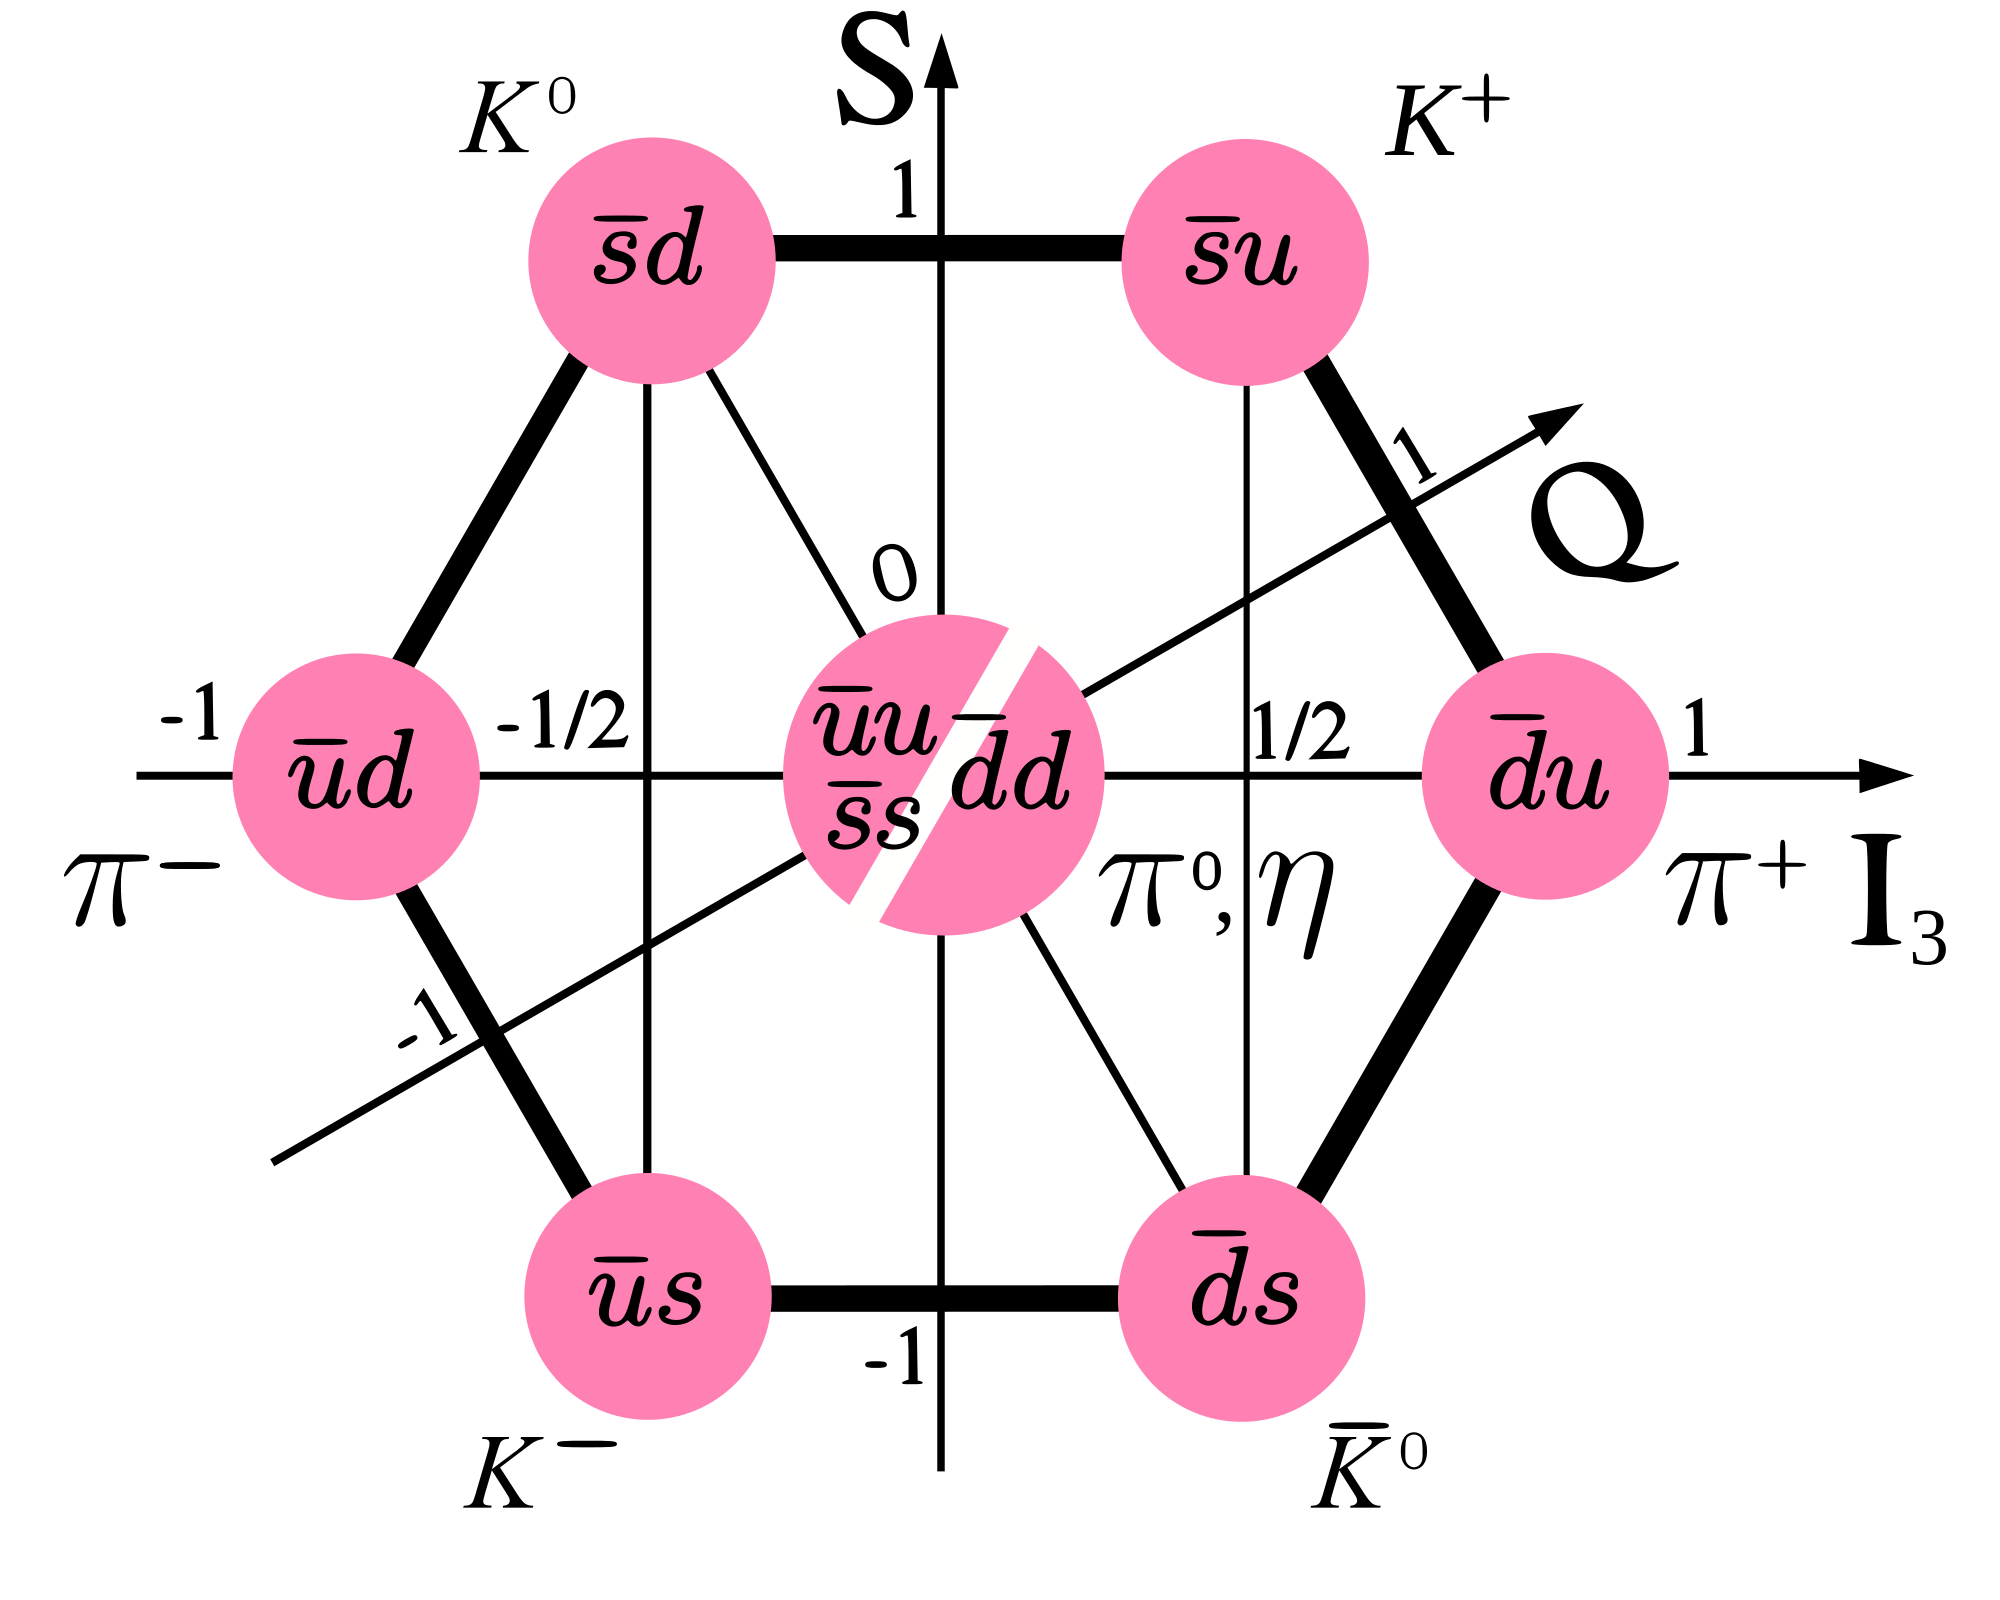
\includegraphics[width=0.45\textwidth]{Chapters/pQCD/Meson-octet_0.png}
  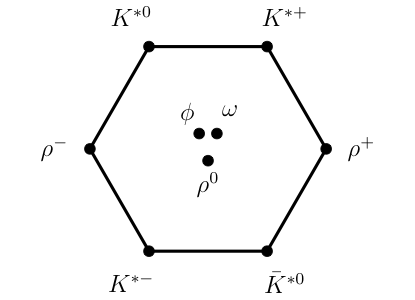
\includegraphics[width=0.45\textwidth]{Chapters/pQCD/Meson-octet_1.png}
 \caption{Left: the pseudo-scalar meson octet. Right: the vector meson octet.}
 \label{fig:mesonoctet}
\end{center}
\end{figure}

As a consequence of the octet structure, Gell-Mann went on to predict in the same paper the existence of
an electrically neutral meson completing the pseudo-scalar meson octet. The $\eta$~meson
was discovered in 1961 by Pevsner and others~\cite{PhysRevLett.7.421}. 

Gell-Mann also pointed out in a 1962 conference that nine known excited
baryons of spin-parity $J^P = 3/2^{+}$ would fit nicely into a decuplet representation of
$SU(3)$ if a tenth baryon carrying strangeness $S=-3$ were to be
found~\cite{1962_GM_omega}. The discovery of the $\Omega^{-}$ baryon in 1964 at
Brookhaven~\cite{omegabaryon} at precisely the mass given by the
theory estimation~\cite{GM_omega,Okubo} sealed the success of the
$SU(3)_F$ flavour symmetry. The complete baryon $J^P = 1/2^{+}$ octet
and $J^P = 3/2^{+}$ decuplet are presented in Figure~\ref{fig:baryonoctet}.

\begin{figure}[h]
\begin{center}
  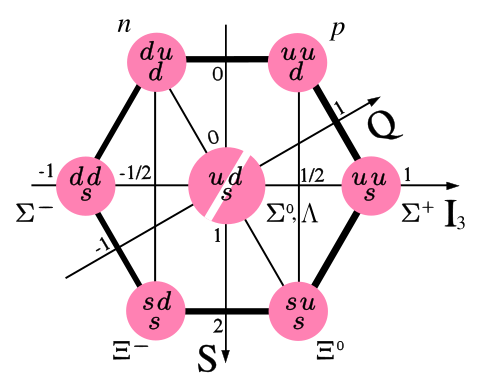
\includegraphics[width=0.45\textwidth]{Chapters/pQCD/Baryon-octet.png}
  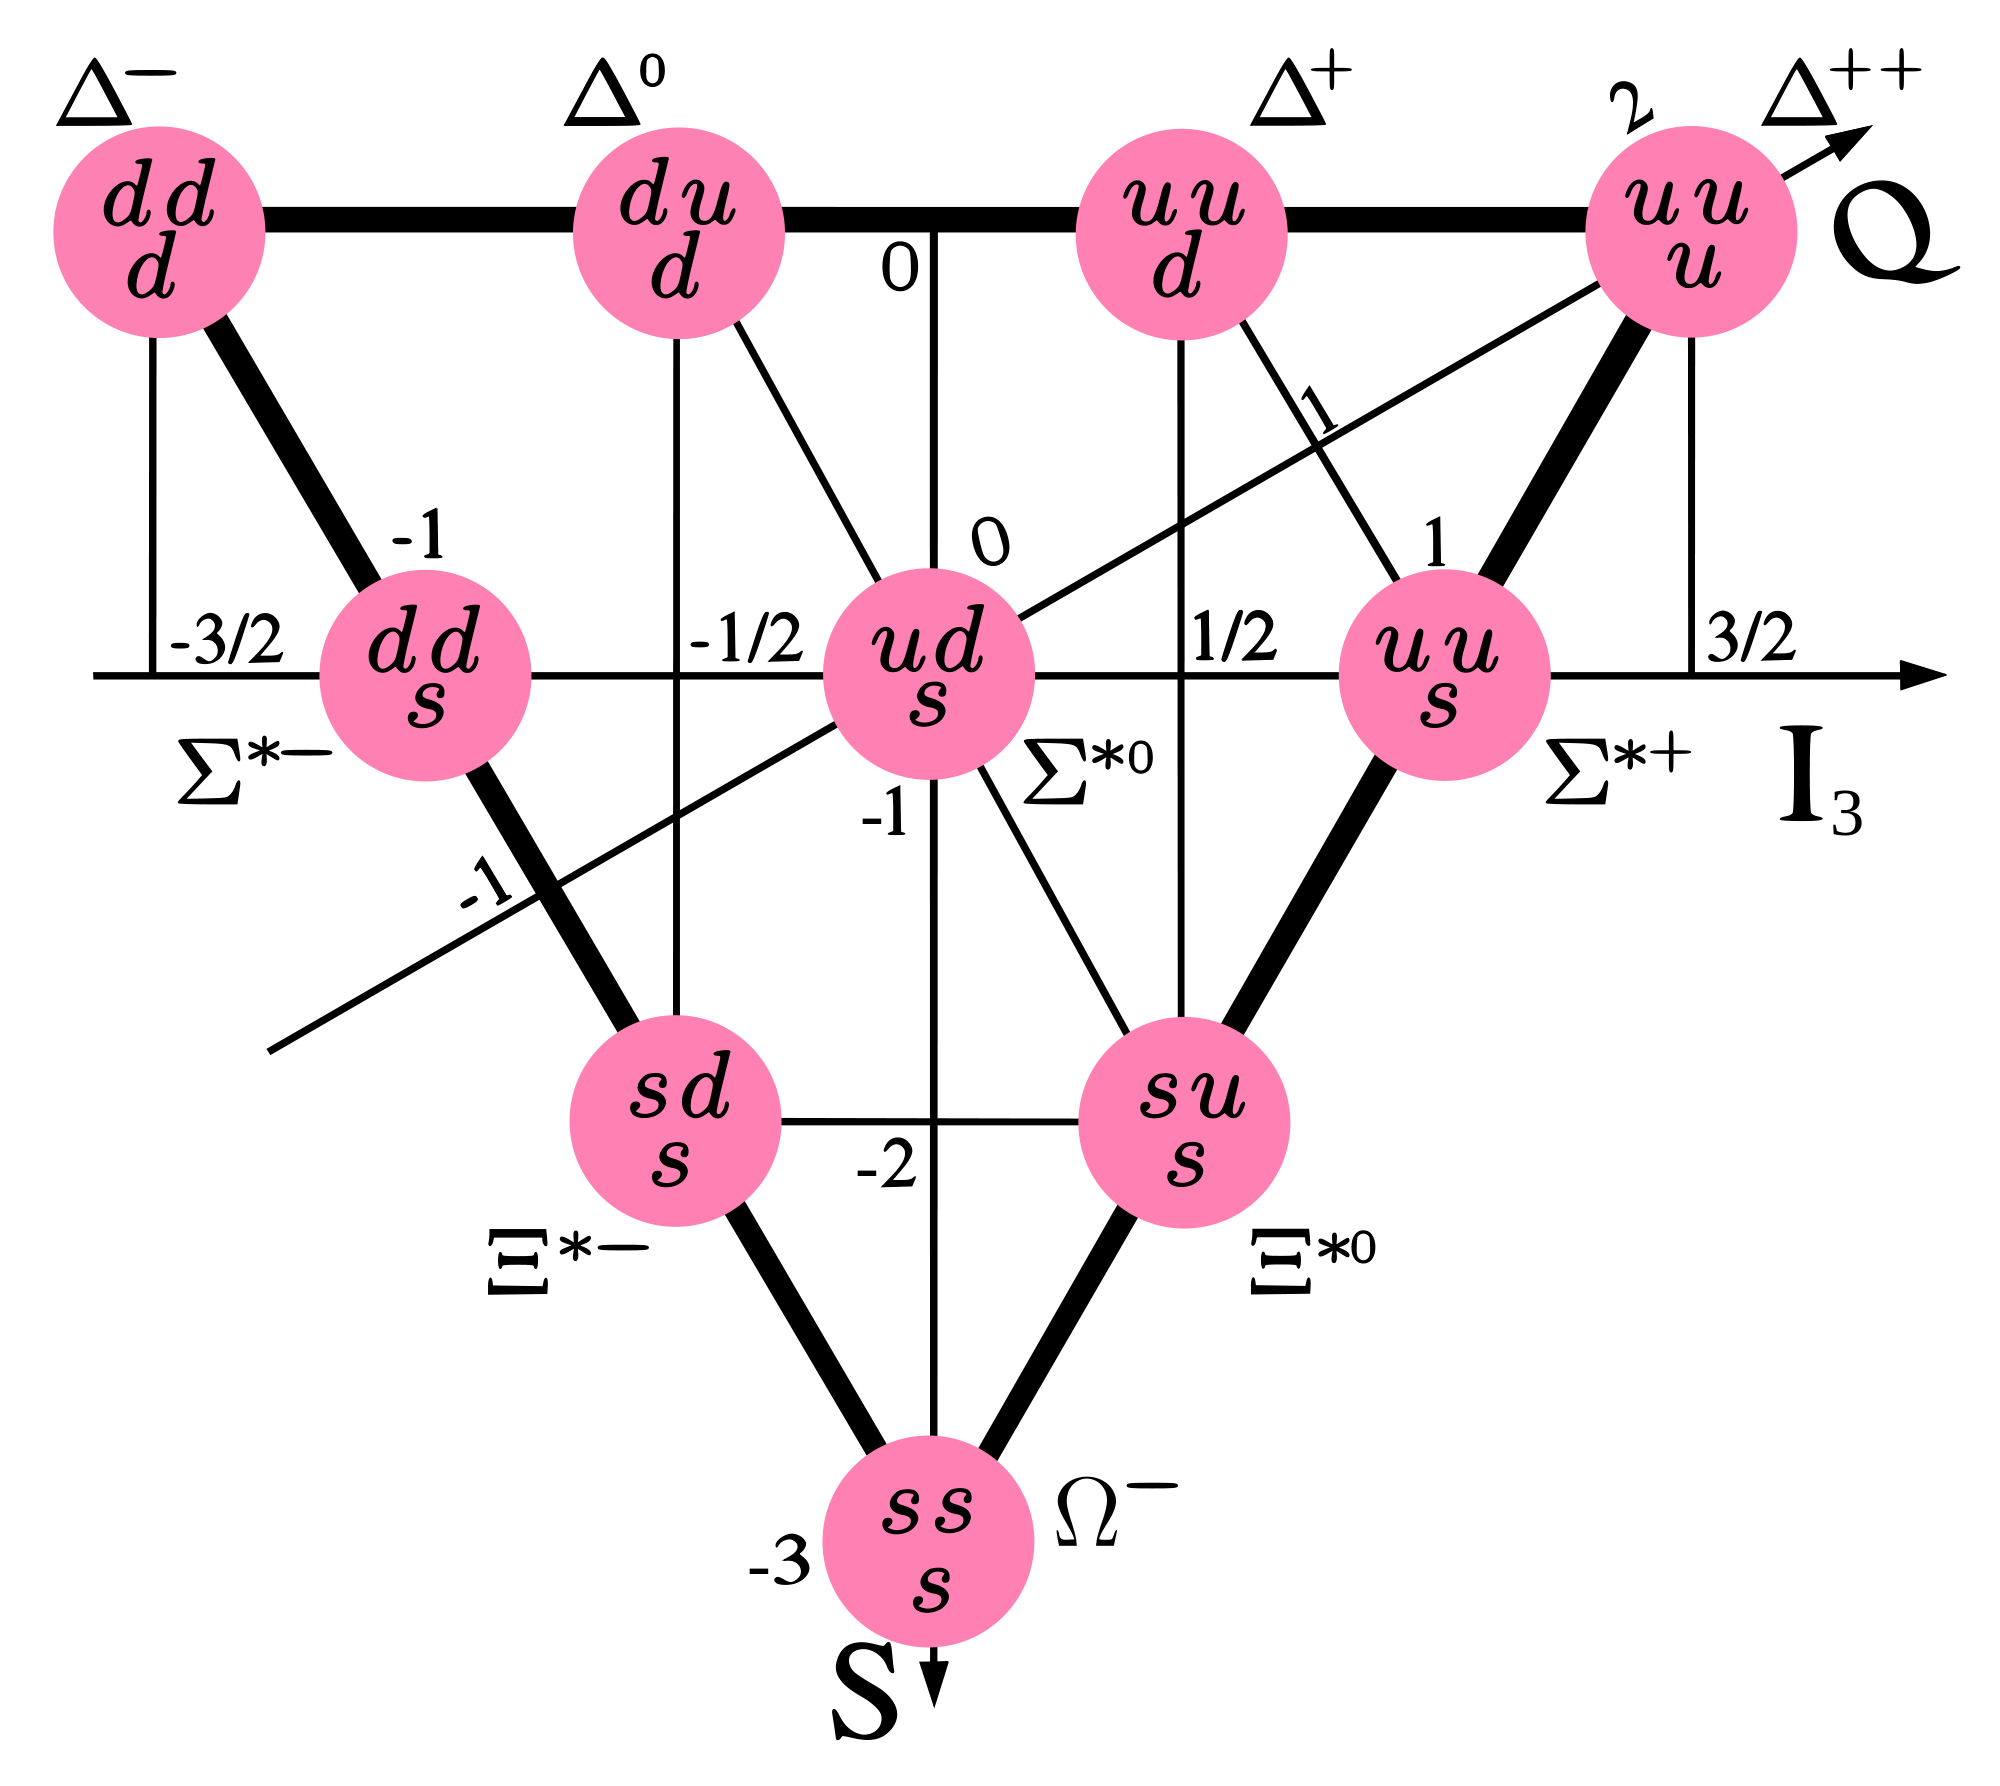
\includegraphics[width=0.4\textwidth]{Chapters/pQCD/Baryon-decuplet.png}
 \caption{Left: the $J^P = 1/2^{+}$ baryon octet. Right: the $J^P =
   3/2^{+}$ baryon decuplet, showing the $S=-3$ baryon $\Omega^-$ at
   the bottom of the decuplet.%  (Note: the change of convention
   % for the orientation of the strangeness axis between left is arbitrary.)
 }
 \label{fig:baryonoctet}
\end{center}
\end{figure}

\subsection{The need for colour}
\label{sec:colour}
By 1964, the static picture of hadrons had emerged. There was an
understanding in the community that a theory of strong interactions
of non-abelian nature
% (likely spontaneously broken, because of the
% differences in masses of the hadrons) 
is underlying, but its dynamics
was yet unknown. What is the force carrier behind the strong
interaction? Where is the triplet of particles of the fundamental
representation of $SU(3)$? These questions would be answered in the
coming ten years with the formulation of the quark model, the parton
picture and
eventually that of QCD.

What I have described here is already a quark
model\footnote{Sometimes, the (u,d,s) model is referred to as
  the 'naive' quark model.}, with three
flavours. Because the masses are not all equal between the
three quark flavours, we can only consider the flavour symmetry as
approximate. % I would like to raise two other problems with the quark model as
% it stands at this point:
% One big problem in the hadron spectroscopy comes from the statistics
% obeyed by the
%. Indeed, according to the

Furthermore, hadron spectroscopy seems to be driven by the wrong
statistics. Indeed, according to spin-parity of the baryon decuplet,
$J^{P} = \frac{3}{2}^{+}$, the baryon wave functions should be fully antisymmetric. Let us consider
the states $\Omega^{-}, \Delta^{++}$ and $\Delta^{-}$ at the
corners of the decuplet diagram (cf. Figure~\ref{fig:baryonoctet} right):
\begin{align*}
&\ket{\Delta^{++}(S_{z}=3/2)} \sim \ket{u^\uparrow u^\uparrow
  u^\uparrow},\\
&\ket{\Delta^{-}(S_{z}=3/2)} \sim \ket{d^\uparrow d^\uparrow
  d^\uparrow},\\
&\ket{\Omega^{-}(S_{z}=3/2)} \sim \ket{s^\uparrow s^\uparrow s^\uparrow}
\end{align*}
We see that each state has three identical spin-aligned quarks. Furthermore, the
decuplet states are at the fundamental level ($L=0$), and all relative
angular momenta between quarks equal to zero. This leads to a fully
symmetric wave function and therefore the three
states obey the wrong statistics. In other words, Pauli's exclusion principle should preclude these particle from existing. 

To anti-symmetrise the baryon states, one can introduce an additional
quantum number, \textit{colour}, such that in this picture, a sum of
permutations of the colour states are contributing to the observed
baryon. In the case of $\Delta^{++}$, one has:
\begin{equation}
\ket{\Delta^{++}} \sim \frac{1}{\sqrt{6}}\epsilon^{\alpha\beta\gamma}\ket{u_{\alpha}^\uparrow u_{\beta}^\uparrow
  u_{\gamma}^\uparrow},
\end{equation}
Where the sum is implicit (using Einstein's convention) over
colours, and $\epsilon^{\alpha\beta\gamma}$ is the fully
anti-symmetric Levi-Civita tensor. One sees that at least three
colours are needed to have an antisymmetric state. In this
description one can construct 9 different colour combinations for the
$q\bar{q}$ meson wave functions, out of which only 3 seem to exist. 
Also, the fact that only $q\bar{q}$ and $qqq$ states are observed is 
a puzzle. 

These two problems are solved by the ad-hoc colour
\textit{confinement hypothesis} that should have a dynamical nature:
since quarks carry colour and hadrons are colour-singlet 
states, there must be a mechanism responsible for equilibrating the
colour content in the final state. Nowadays the colours used for
quarks are
\color{red}\textbf{red}\color{black},~\color{green}\textbf{green}
\color{black}and 
\color{blue}\textbf{blue}\color{black}, while
anti-\color{red}\textbf{red}\color{black},~anti-\color{green}\textbf{green} \color{black} and
anti-\color{blue}\textbf{blue}\color{black}~are antiquark colours. The
choice is of course arbitrary, but inspired by the analogy of
colour-singlet states appearing white.

\subsection{Evidence for quarks}
\label{sec:quarks}
The quark picture put forth in the early sixties did not get
firm approval in the community immediately. Quarks were lacking an
experimental evidence, and it was by no means clear that experiments
would ever be able to produce fractional electric charge particles. The
evidence came from a series of deeply inelastic electron-nucleon
scattering experiments performed
by the SLAC-MIT collaboration (for which Friedman, Kendall and Taylor were awarded the Nobel Prize in Physics in 1990).


The impact of deep inelastic scattering experiments on the inception
of chromodynamics is considerable, and the basics are
presented here. Let us consider the typical reaction $e^{-}+p \to e^{-}+X$ where X is
any number of hadronic remnants in the final state. The diagram in Figure~\ref{fig:dis_test} lays out the kinematics
of the reaction.
\begin{figure}[h]
\begin{center}
  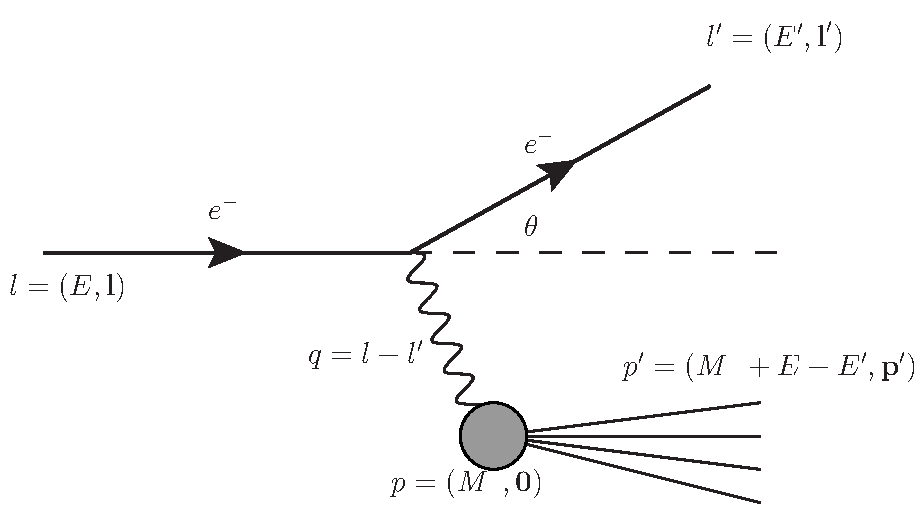
\includegraphics[width=0.7\textwidth]{Chapters/pQCD/DIS_test.pdf}
 \caption{Deep inelastic $e^{-}p$ scattering. A photon is exchanged
   and a hadronic final state X is formed.}
 \label{fig:dis_test}
\end{center}
\end{figure}

The initial high-energy electron scatters off a proton of mass $M$
and four momentum $p$, via the exchange of a space-like virtual
photon. In the final state, $\theta$ is the electron scattering angle, the electron has a
four-momentum $l'$ and the hadronic system has invariant mass $W$. The
energy transfer between the electron and the hadronic system is $\nu$:

\begin{equation}
\nu = E - E' = \frac{q\cdot p}{M}
\end{equation}

and the virtuality of the photon, i.e. its squared momentum transfer
$Q^{2}$ is defined as:
\begin{equation}
Q^{2} = -(l - l^{'})^{2} = 2M\nu + M^{2} - W^{2} \leq
2M\nu .
\label{eq:qsquare}
\end{equation}
In the elastic scattering, where $X$ is made of the initial scattered proton, the rightmost terms of Equation~\ref{eq:qsquare} would turn into an equality.
We can now introduce the so called Bjorken-$x$, $x_{B}$, that would represent how much the
process deviates from the elastic scattering
\begin{equation}
x_{B} = \frac{Q^{2}}{2M\nu}, \hspace{1cm} 0 \leq x_{B} \leq 1.
\end{equation}

 In this sense, when the momentum exchange is negligible, the
final-state invariant mass $W$ tends to $M$, and $x_{B} = 1$
(elastic scattering). In turn, small values of $x_{B}$ correspond to
high momentum exchange, $Q^{2} \gg M \nu$. To test if a target proton contains inner degrees of
freedom, one can consider the cross-section for scattering of a lepton
off a spin-1/2 fermion of mass $M$, charge e$_q$ and specific to
the case of non pointlike particles\footnote{A textbook example of
  this calculation is available for example in Appendix F of~\cite{qcd_book}.}. A double-differential cross
section can be derived as a function of two \emph{structure functions} $W_1$ and $W_2$~\cite{qcd_book}:
\begin{equation}
\frac{d^{2}\sigma}{dQ^{2}d\nu} = \frac{4\pi\alpha^{2}_{QED}}{Q^{4}}\frac{E'}{E}\left( W_2(Q^{2},\nu)\rm{cos}^2\frac{\theta}{2} +
    2W_1(Q^{2},\nu)\rm{sin}^2\frac{\theta}{2} \right)
\label{eq:QED_DIScrosssection}
\end{equation}

In Equation~\ref{eq:QED_DIScrosssection}, the scattering process occurs
via the exchange of a photon, hence the QED coupling constant
$\alpha_{QED}$. Equation~\ref{eq:QED_DIScrosssection} assumes the hypothesis that a nucleon is an extended particle,
composed of several pointlike particles with electric charge $e_i$. One then defines \emph{parton
distribution functions} (PDF) $f_i(x_i)$, representing the probability
that the struck
\textit{parton} carries a momentum fraction $x_i$ of the
nucleon. Thus, the structure constants built with the
parton distribution functions are: 
\begin{equation}
W_1(Q^2,\nu)=\displaystyle\sum_{i}e^{2}_{i}f_{i}(x_{B})\frac{1}{2M}
\end{equation}
and
\begin{equation}
W_2(Q^2,\nu)=\displaystyle\sum_{i}e^{2}_{i}f_{i}(x_{B})\frac{x_{B}}{\nu}.
\end{equation}
One can absorb $M$ and $\nu$ into these definitions to parameterize the lepton-nucleon cross section in deep inelastic scattering (DIS) with two functions that depend only on how the momentum is shared between the nucleon constituents:
\begin{equation}
F_1\equiv M_{h} W_1
=\frac{1}{2}\displaystyle\sum_{i}e^{2}_{i}f_{i}(x), \hspace{1cm}
F_2\equiv \nu W_2 =\displaystyle\sum_{i}e^{2}_{i}xf_{i}(x).
\end{equation}

The fact that DIS processes depend only on $x$, a dimensionless
parameter, translates into the independence of the structure function
F$_2$ with the Q$^{2}$ of the reaction. This is called \textit{Bjorken
  scaling}, and is the main feature of the parton
model~\cite{webber3}. This scaling behaviour was first measured by the
MIT-SLAC collaboration in 1970. Figure~\ref{fig:F2scaling} shows the
$F_{2}$ structure function, as a function of $x$, for various 
DIS energies on a proton target. The scaling here manifests itself in
the form of this universal curve holding for very different values of
$Q^{2}$. This is a definite proof of the existence of pointlike
consituents at these energy scales, as the presence of non-pointlike
particles would make structure functions depend on  $Q/Q_{0}$, with
$1/Q_{0}$ the typical size of the non-pointlike object.

\begin{figure}[h]
\begin{center}
  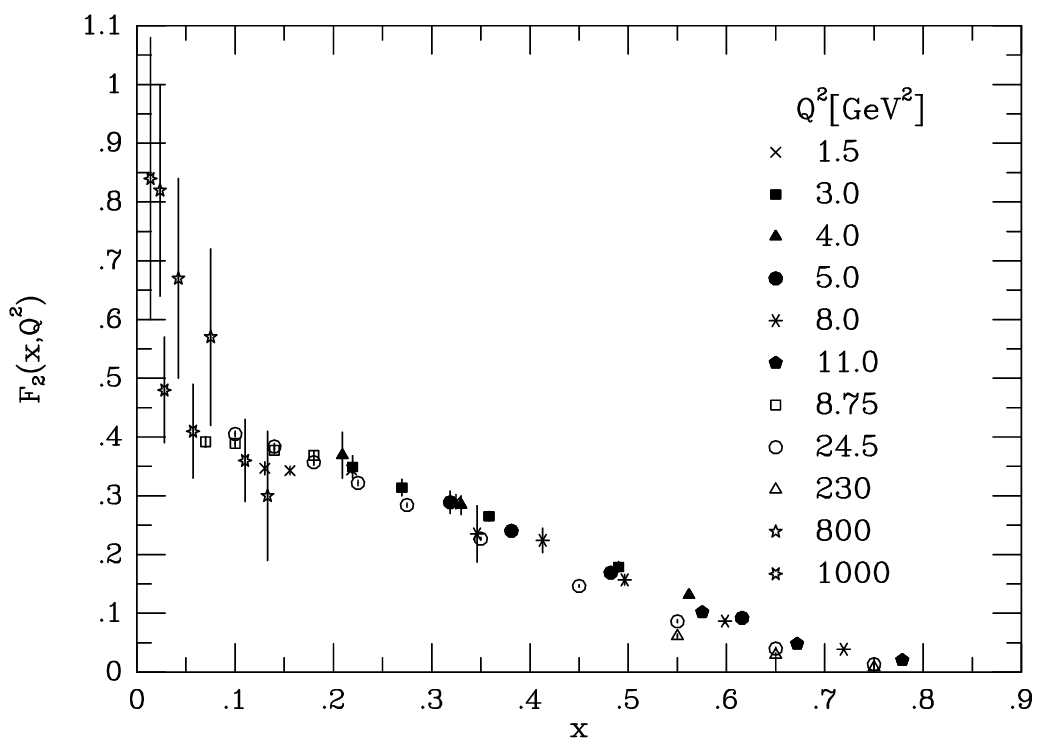
\includegraphics[width=0.7\textwidth]{Chapters/pQCD/F2scaling.png}
 \caption{Structure function $F_{2}$ as a function of $x$. Emergence
   of scaling at various $Q^{2}$ energies in proton DIS. Compilation
   of PETRA data taken from~\cite{webber3}.}
 \label{fig:F2scaling}
\end{center}
\end{figure}

\subsection{On the verge of a revolution}
\label{sec:verge}
I have presented the inherent colour in the quark model, and how
quarks have been discovered in early DIS experiments% , leading to a
% partonic picture of the quark model
. There are many
aspects of the puzzle of this pre-QCD era which 
have not been dealt with. For example, I did not mention that structure
functions can be expressed in terms of the quark -- and anti-quark --
densities inside the target hadron. For example for $u$ and $d$ quarks one
has:
\begin{equation}
u= u_{\rm p}(x) \hspace{0.5cm}d= d_{\rm p}(x) \hspace{0.5cm}\bar{u}= \bar{u}_{\rm p}(x) \hspace{0.5cm}\bar{d}= \bar{d}_{\rm p}(x) \hspace{0.5cm}
\end{equation}

In this sense, doing a DIS experiment allows one to measure the PDFs of
each quark flavour. In the case of electron-deuterium scattering for example, one can
write the two $F_2(x)$ of electron-proton and electron-neutron processes:
\begin{eqnarray}
F_{2}^{ep}(x) &=& x\left[ \frac{4}{9}(u+\bar{u}) + \frac{1}{9}(d+\bar{d}) \right]\\
F_{2}^{en}(x) &=& x\left[ \frac{1}{9}(u+\bar{u}) + \frac{4}{9}(d+\bar{d}) \right].
\end{eqnarray}

These two can be averaged\footnote{The average in any nucleus is
  $F_{2}^{eA}(x) = Z F_{2}^{ep}(x) + (A-Z) F_{2}^{en}(x)$.} to compute
the $F_{2}^{eN}$ of the deuteron:
\begin{equation}
F_{2}^{eN}(x) = \frac{5}{18}x\left(u  + \bar{u} + d + \bar{d}  \right).
\end{equation}
Implicitly, each parton distribution contains a contribution from the three
\textit{valence} quarks of a nucleon, as well as \textit{sea} quarks
and anti-quarks coming from vacuum excitations. It follows that integrating over $x$
should give the total fraction of momentum carried by quark degrees of
freedom. One finds experimentally:

\begin{equation}
\int^{1}_{0} dx \: F_{2}^{eN}(x) = \int^{1}_{0} dx\:
\frac{5}{18}x\left(u  + \bar{u} + d + \bar{d}  \right) \simeq 0.5 \label{eqhalftheproton}
\end{equation}


This puzzling result indicates that charged partons in the deuterium nucleus (valence quarks $+$
sea quarks and anti-quarks) carry nearly half of the total
momentum. The rest has to be carried by other particles trapped in the
nucleon, which do not carry electric charge since their momentum is not
probed with electromagnetic processes such as DIS. % Neutrino-nucleon
% reactions did not help in reconciling this result with expectation
% (integral equals one), so the invisible momentum carriers are also
% neutral in terms of weak charge.
These are in fact the \emph{gluons}, which
will be discovered later.

A second puzzle is related to the Bjorken scaling presented in the
parton model, in Section~\ref{sec:quarks}. Assuming that one increases the energy indefinitely, a
DIS experiment would eventually reach the scale of vacuum
fluctuations. In other terms, more partons compose the nucleon at very
high $Q^{2}$ values, and hence more partons share the momentum of the
nucleon, leading to softer structure functions at high-$Q^{2}$. This
is a \textit{violation} of the Bjorken scaling at high energy. Anticipating
that the decrease in structure functions is proportional to the
coupling between partons~\cite{qcd_book}, one has:

\begin{equation}
\frac{dF}{F} \:\sim\: \alpha\frac{dQ^{2}}{Q^{2}} \hspace{1cm}\Longrightarrow\hspace{1cm}
\frac{d\,\textrm{ln}F}{d\,\textrm{ln}Q^{2}} \:\sim\: \alpha
\label{eq:couplingeq}
\end{equation}

If this interaction between partons were to be electromagnetic, the
obtained $\alpha$ would be quite small (reminder: $\alpha_{QED}\approx$
1/137). Although Figure~\ref{fig:F2scaling} largely exhibits the
scaling of structure functions (all lining up on top of each other in
a large $x$ range and for various $Q^2$ values), let us look at
some of the high-$Q^{2}$ points (provided the error bars are small
enough), to see what the Equation~\ref{eq:couplingeq} yields. Using the values at $x_{B}$ =
0.55 of Figure~\ref{fig:F2scaling}, $F_{2}(x=0.55, Q^{2}=230~$GeV$^{2})\approx$ 0.063, and $F_{2}(x=0.55, Q^{2}=24.5~$GeV$^{2})\approx$ 0.086, we get the large value of\footnote{I have used
  \href{http://rhig.physics.yale.edu/~ullrich/software/xyscan/}{http://rhig.physics.yale.edu/$\sim$ullrich/software/xyscan/}.}: 

\begin{equation}
\left| \frac{\Delta\,\textrm{ln}F}{\Delta\,\textrm{ln}Q^{2}} \right|
\:\sim\: 0.14
\end{equation}

\vspace{0.5em}
\begin{center}
  \fbox{
    \parbox{0.9\textwidth}
    {\textsf {We have witnessed the existence of a strong interaction between partons. The quark model gave us a group structure, $SU(3)$,
and a quantum number, colour. Now that the symmetry of the
group seems to be due to three colours (and not flavours), that leaves no clear limit
on the number of quarks. The next section will indeed introduce extra flavours.
% As history has it~\cite{SLACbeamline}, Glashow, Iliopoulos and Maiani put forth in 1970 a mechanism explaining the mixing of flavours through an electroweak flavour changing process~\cite{GIM}. The writers of this model were probably the only ones at the time, to call for the existence of more than three quarks. 
We will start by presenting the main theoretical concepts of
QCD, and some experimental confirmations that this is the quantum
theory of strong nuclear interactions.}}} 
\end{center}

% This almost wraps up my review of the pre-QCD era.


 % I will take the renormalisability
% hypothesis for granted, and I will make use of the gauge-invariance
% and refer the reader to textbooks for demonstrations going from the
% abelian case of $U(1)_{QED}$ to the non-abelian Yang-Mills theories
% $SU(2)$ and $SU(3)$.

 % -- but I will leave this discussion here for now.


\section{QCD: Theoretical grounds, experimental milestones}
\label{sec:QCD}
\subsection{The QCD Lagrangian}
\label{sec:lagrangian}
Equation~\ref{eq:qcdlagrangian} introduces the Lagrangian of QCD:
\begin{eqnarray}
\mathcal{L}_{\rm{QCD}}\:&=&\:-\frac{1}{4}F^{A}_{\alpha\beta}F^{\alpha\beta}_{A} +
\sum_{\rm{flavours}}\bar{q}_{a}(i\slashed{D} - m)_{ab}q_{b} +
\mathcal{L}_{\rm{gauge-fixing}} \label{eq:qcdlagrangian}\\
F^{A}_{\alpha\beta} &=& \partial_{\alpha}\mathcal{A}^{A}_{\beta}
- \partial_{\beta}\mathcal{A}^{A}_{\alpha} -
gf^{ABC}\mathcal{A}_{\alpha}^{B}\mathcal{A}_{\beta}^{C} \label{eq:qcdstresstensor}
\end{eqnarray}
\vspace{0.5cm}
The QCD Lagrangian has some similarities with the one of QED, except that:
\begin{itemize}
\item[-] The stress tensors' product $-\frac{1}{4}F^{A}_{\alpha\beta}F^{\alpha\beta}_{A}$ runs over 8 gluon fields, labeled by their colour indices ($A$),
\item[-] There is a non-abelian quadratic term in the stress tensor $F^{A}_{\alpha\beta}$, 
\item[-] There are $N_{\rm f}$ quark fields $q_{a}$ in the
  triplet colour representation,
\item[-] Coupling between fermions and bosons occurs at strength
  $\alpha_{S} \equiv g^{2}/4\pi$, through the following $\bar{q}_{a} \slashed{D}_{ab} q_{b}$ term.
\end{itemize} 

$\slashed{D}$ is the Dirac notation for $\gamma^{\alpha}D_{\alpha}$, the contraction of Dirac
$\gamma^{\alpha}$ matrices and the covariant derivative $D_{\alpha}$, defined as:

\begin{eqnarray}
(D_{\alpha})_{ab} \: &=& \: \partial_{\alpha}\delta_{ab} +
ig\left(t^{C}\mathcal{A}^C_{\alpha}\right)_{ab}\\
(D_{\alpha})_{AB} \: &=& \: \partial_{\alpha}\delta_{AB} + ig\left(T^{C}\mathcal{A}^C_{\alpha}\right)_{AB}
\end{eqnarray}

$f^{ABC}$ are numbers called the \emph{structure constants} of $SU(3)$ (the
terminology has nothing in common with structure functions seen in
Section~\ref{sec:strong}) and connects with $t$ and $T$ colour matrices in either the fundamental or
the adjoint representation, respectively:
\begin{equation}
\left[ t^{A}, t^{B}\right] = i f^{ABC}\,t^{C}, \hspace{1cm} \left[ T^{A}, T^{B}\right] = i f^{ABC}\,T^{C}
\end{equation}

In group theory such commutation relations ensure completeness (as is needed in quantum mechanics), and the normalisation of $t$
matrices follows:
\begin{equation}
\mathsf{Tr}\: t^{A}t^{B} = T_{R}\: \delta^{AB}, \hspace{0.5cm} T_{R} = \frac{1}{2}.
\end{equation}

From colour matrices one also gets the \emph{colour factors}, generalised to
$SU(N)$:
\begin{eqnarray}
\displaystyle\sum_{A}t_{ab}^{A}t_{bc}^{A} &=&
C_{F}\,\delta_{ac},\hspace{0.5cm} C_{F} = \frac{N^{2}-1}{2N}\\
\mathsf{Tr}\: T^{C}T^{D} &=& C_{A}\,\delta_{CD},\hspace{0.5cm} C_{A}=N
\end{eqnarray}
which, in the case of $SU(3)$, are $C_{F}=4/3$ and $C_A = 3$.

\subsection{The running of the coupling constant
  \texorpdfstring{$\alpha_{S}$}{as}}
\label{sec:running}
One of the ways often used to bring up the notion of the running of
$\alpha_{S}$ (for instance in \cite{webber1}) is to consider a dimensionless physical observable $R$ which depends on an energy scale $Q$ that is much larger than the masses $m$ in consideration. We shall see such a quantity at the end of this section. 

Dimensional analysis suggests that $R$ should be independent of $Q$, when much larger than $m$. This does not hold in quantum field theory, because the perturbative development in $\alpha_S$ requires \emph{renormalization}. This procedure introduces a new scale $\mu$, where the subtraction removing divergences is performed. 

% The $R$ quantity can indeed be developed as a perturbative expansion in orders of a \emph{bare} coupling $\alpha_{S,\rm{bare}}$. This coupling differs from the $\alpha_S = g^2 4\pi  $ introduced in the Lagrangian in that $g$ was in fact a \textit{renormalised coupling}, i.e. a constant, while the bare coupling is a function of some energy scale $\mu$ above which one can make a perturbative expansion with it. 

Dimensional analysis suggests again that $R$ depends on $Q^2/\mu^2$ and on $\alpha_S$, which itself depends on $\mu$. Since $\mu$ is arbitrary, $R$ cannot depend on $\mu$, and it follows that: 
\begin{equation}
\mu^{2}\,\frac{d}{d\mu^{2}}R\left(\frac{Q^{2}}{\mu^{2}},\alpha_{S}\right)
\,\equiv\, \left( \mu^{2}\frac{\partial}{\partial\mu^{2}} + \mu^{2}\frac{\partial\alpha_{s}}{\partial\mu^{2}}\frac{\partial}{\partial\alpha_{S}}  \right)\,R = 0.
\end{equation}

% look at the $R$ cross section ratio:
%
%\begin{equation}
%R\: \eqdef \:\, \frac{\sigma(e^{+}e^{-}\to\textrm{hadrons})}{\sigma(e^{+}e^{-}\to\mu^{+}\mu^{-})}.
%\end{equation}
%
%$R$ is the ratio of cross sections for hadron production and dimuon
%production at electron-positron colliders. Since both the numerator
%and denominator have the dimension of a cross section, this is a
%dimensionless parameter. But experimentally one sees it is depending on some energy scale larger
%than quark masses, $Q \gg m$, as can be seen in
%Figure~\ref{fig:repem}.
%\begin{figure}[h]
%\begin{center}
%  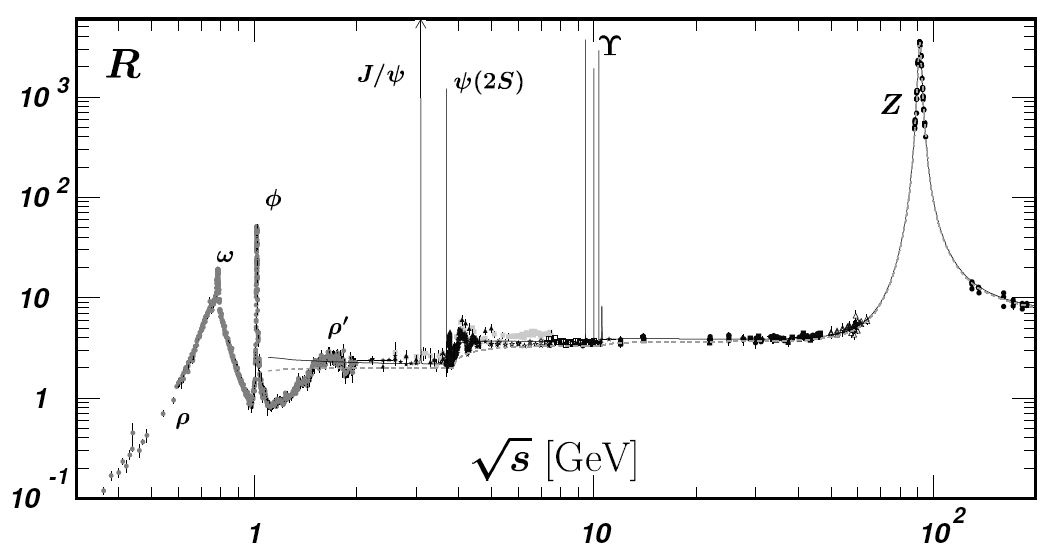
\includegraphics[width=0.8\textwidth]{Chapters/pQCD/repem.png}
% \caption{R ratio of electron positron cross section to hadrons and
%   leptons, as a function of centre-of-mass energies.}
% \label{fig:repem}
%\end{center}
%\end{figure}
%
%We see from the plot that $R$ increases with centre-of-mass energy. % in steps that are delimited by
%% approximately the centre-of-mass energy needed to produce a new quark
%% flavour.
%This behaviour is problematic, since dimensional analysis
%tells us that $R$ should be independent of the energy scale, hence
%constant when increasing the centre-of-mass energy.

% This behaviour is regularised with the formalism of renormalisation. 

% In quantum field theories, % In order to avoid discussion of renormalisation theory, I'll assume
% that $R$, which in principle should not depend of any energy scale $Q^{2}$,
% can become non-dimensional using the tools of dimensional regularisation,
% so that $R$ is now a function of the ratio $Q^{2}/\mu^{2}$.

%With
%$\alpha_S$ being a function of $\mu$ we have for $R$:
%\begin{equation}
%R \equiv R\left(\frac{Q^{2}}{\mu^{2}},\alpha_{S}(\mu)\right),
%\end{equation}
%but at a given (constant) coupling $\alpha_S^{r}$ (the one entering
%the Lagrangian), $R$ does not depend strictly on $\mu$, and can be
%expressed as $R(Q^{2}/\mu,\alpha_{S})$ such that:
%\begin{equation}
%\mu^{2}\,\frac{d}{d\mu^{2}}R\left(\frac{Q^{2}}{\mu^{2}},\alpha_{S}\right)
%\,\equiv\, \left( \mu^{2}\frac{\partial}{\partial\mu^{2}} + \mu^{2}\frac{\partial\alpha_{s}}{\partial\mu^{2}}\frac{\partial}{\partial\alpha_{S}}  \right)\,R = 0.
%\end{equation}

This partial differential equation can be simplified introducing
the following:
\begin{equation}
\tau = \textrm{ln}\left( \frac{Q^{2}}{\mu^{2}} \right),\hspace{1cm}\beta(\alpha_{S})=\mu^{2}\,\frac{\partial\alpha_{S}}{\partial\mu^{2}}
\end{equation}
We now have a \textit{renormalisation group equation} for $R$:
\begin{equation}
\left( -\frac{\partial}{\partial\tau} +
  \beta(\alpha_{S})\frac{\partial}{\partial\alpha_{S}}\right)R\:=\:0.
\end{equation}

This can be solved by defining a coupling varying with the scale, the
\emph{running coupling}:
\begin{equation}
\tau = \int_{\alpha_{S}(\mu)}^{\alpha_{S}(Q)} \frac{dx}{\beta(x)},
\end{equation}
and the way $\alpha_{S}$ varies is determined by the $\beta$
function. Anticipating that a determination of $\alpha_{S}$ with the
$\beta$ function is based on
an infinite series of ever more complicated diagrams revolving around
gluon self interactions and quark loops, let us just jump to the
result and say that $\beta$ at first order in $\alpha_{S}$ (\textit{leading
order}, or LO) is given by:
\begin{eqnarray}
\beta(\alpha_{S}) &=& -b \alpha^{2}_{S}(1 +\mathcal{O}(\alpha_{S}))\\
\vspace{0.5cm}
b &=& \frac{11 C_{A} - 2 N_{f}}{12\pi} > 0
\end{eqnarray}
where $C_A=3$ and $N_f$ the number of active flavours. The $\beta$ function values decrease as
$\alpha_{S}$ increases, and
the first order $-b$ parameter is \textit{negative}\footnote{That is,
  as long as the number of active quark flavours is $N_f < 16$.}, contrary to the two electroweak constants. For QED,
$\beta(\alpha_{QED})=\alpha_{QED}^{2}/3\pi$. It is positive, such that
the coupling increases when one resolves the charged particle with higher
and higher energies. Inversely, for quantum chromodynamics, the
coupling decreases as energy increases: this is known as \emph{asymptotic
freedom}.

Modern measurements of $\alpha_S(Q)$ will be shown in
Section~\ref{sec:alphasrunning} and we will see how well they match
with the theoretical prediction of running $\alpha_S$. 
I have decided to limit myself to the running of the coupling and
the basic structure of the Lagrangian, for the following reasons:
\begin{itemize}
\item[-] These two points are fundamental for the building of QCD, and
  make it a unique theory,
\item[-] the non-abelian term in the Lagrangian is crucial for the
  appearance of this asymptotic freedom property,
\item[-] the dynamical evolution of the coupling
  sets the basis to turn to \emph{deconfinement}.
\end{itemize}

The rest of this section will be devoted to present experimental
successes, or milestones, of QCD. 

Let us look first at a concrete quantity, that is the ratio $R$ of
cross sections for hadron production and dimuon production in
$e^{+}e^{-}$ annihilation:
\begin{equation}
R\: \eqdef \:\, \frac{\sigma(e^{+}e^{-}\to\textrm{hadrons})}{\sigma(e^{+}e^{-}\to\mu^{+}\mu^{-})}.
\end{equation}

This quantity, as plotted in Figure~\ref{fig:repem}, varies mildly and
continuously as a function of \s\ above 5~GeV, in a way that is well
reproduced by the running coupling constant (see~\cite{Agashe:2014kda}, Section
9.2.1). It also reveals striking features: resonances, and steps that are thresholds
for the production of new quarks, that I shall discuss in the next section. 

\begin{figure}[h]
\begin{center}
  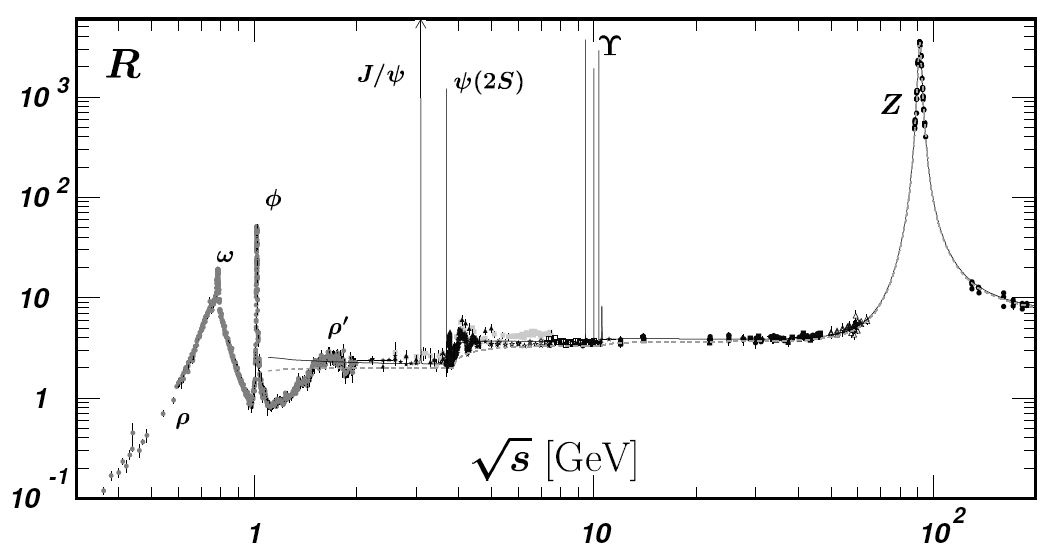
\includegraphics[width=0.8\textwidth]{Chapters/pQCD/repem.png}
 \caption{R ratio of electron positron cross section to hadrons and
   leptons, as a function of centre-of-mass energy.}
 \label{fig:repem}
\end{center}
\end{figure}

% By essence, the theory is a very
% rich one, and that's maybe where the bat hurts: if one tries to
% develop calculations outside of the perturbative regime, as in the
% case of hadronisation, one finds out fast that a non-perturbative
% treatment for QCD is hopeless. Along the same lines, perturbative QCD
% is essential for high-energy physics, in that most of the corrections
% to processes such as $t$ quark production, Higgs properties, exotic
% physics' searches, ... are all entitled to QCD calculations. One can
% compute QCD processes at leading order, or next-to-leading order, or
% maybe more. But eventually, the computation of the next order relies
% on the knowledge of what is the scale of the next-order effects, and what is going to be size of the coupling for these
% higher order processes. So it seemed to me as the non-Abelian nature
% of $\mathcal{L}$ and the
% running of $\alpha_{S}$ were all I needed for now. When I will be looking at nuclear interactions the picture
% will complexify with collectivity and finite-temperature QCD, but for now,
% I should wrap up the story, pay respects to the November Revolution,
% and salute a few famous measurements that gave to this revolutionary
% theory its full glory.

\subsection{The November Revolution}
\label{sec:november}

In Section~\ref{sec:verge}, I have argued that even though the group
theory grounds were there for QCD to be built already in the sixties, there was a lot
of skepticism regarding the existence of quarks, as well as the
number of quark flavours. At the same time, a large portion of the
theoretical physics community was working on the weak interaction
unification with QED and the renormalisability of quantum gauge field
theories. On the experimental side, strange mesons and baryons were
discovered, and their spectroscopy was well studied. The $s$ quark
mass being presumably heavier than the other two known quarks, it was
clear that hadrons carrying one or more units of strangeness would be
rather unstable. Indeed, the $\Xi$ baryons and $\Omega^{-}$ were
discovered through decay processes. But some transitions, namely the
ones with $\Delta S = 2$ remained elusive. Using the framework of
current algebra, Glashow and Bjorken put out the idea of a
\textit{fourth} quark, the charmed quark, already in 1964. The idea
was to enforce an analogy between the weak leptonic current and weak
hadronic current: if two weak lepton doublets exist, ($e$,$\nu_{e}$)
and ($\mu$,$\nu_{\mu}$), there had two be two weak doublets for quarks
as well~\cite{lai}. 

One of the doubts on the existence of quarks, before DIS experiments
came to light, was the fact that the $SU(3)_{F}$ flavour symmetry of the quark
model was a \textit{global symmetry}~\cite{luigi_gauge}. In this sense, the free fermion
fields for $SU(3)_{F}$ quarks $q_{i}(x)$ are such that:
\begin{equation}
\chi(x) = \begin{pmatrix} q_{u}(x) \\ q_{d}(x) \\ q_{s}(x) \end{pmatrix}
\hspace{1cm} \bar{\chi}(x) = \begin{pmatrix} \bar{q}_{u}(x) &
  \bar{q}_{d}(x) & \bar{q}_{s}(x) \end{pmatrix}
\end{equation}
and the Lagrangian for the three free fields is 
\begin{eqnarray}
\mathcal{L} &=& \displaystyle\sum_{i=u,d,s} \bar{q}_{i}(x)\left(
  i\gamma^{\mu}\partial_{\mu} - m\right)q_{i}(x), \\
&=& \bar{\chi}(x)\left(  i\gamma^{\mu}\partial_{\mu} - m\right)\chi(x).
\end{eqnarray}
Let us express the effect of $V$, a $U(3)$ transformation:
\begin{eqnarray*}
\chi(x) &\to& V\chi(x), \\
\bar{\chi}(x) &\to& \bar{\chi}(x)V^{\dagger}, \\
\mathcal{L} &\to& \bar{\chi}V^{\dagger} \left(
  i\gamma^{\mu}\partial_{\mu} - m \right) V\chi(x) = \mathcal{L}.
\end{eqnarray*}
Given that $U(3) = SU(3) \times U(1)$, such transformations are
unitary 3$\times$3 matrices, with unit determinant. This is the
$SU(3)$ generalised isotopic spin
symmetry of Gell-Mann's Eightfold Way~\cite{eightfoldway}, only
if the quark masses were equal! Entering quark masses would strongly hurt the symmetry to the point where it is
explicitly broken, and as Gell-Mann puts it in~\cite{eightfoldway}, 
\begin{quote}
\textsf{In the limit of unitary symmetry and with the mass of these vector
mesons "turned off'', we have a completely gauge-invariant and minimal
theory, just like electromagnetism. When the mass is turned on, the
gauge invariance is reduced (the gauge function may no longer be
space-time-dependent) but the conservation of unitary spin remains
exact. [...] there are also the many symmetry rules associated with
the unitary spin. All of these are broken, though, by whatever
destroys the unitary symmetry, and it is a delicate matter to find
ways in which these effects of a broken symmetry can be explored experimentally.}
\end{quote}

From there, we can easily imagine what harm it would do to include a
fourth, heavier quark in any such model. In a quite different attempt
to understand flavour-changing currents, Glashow, Iliopoulos and
Maiani~\cite{GIM_mechanism}, suggested in 1970 a mechanism which explains how
the flavour changing process $K^{0}\to \mu\mu$ is naturally rare. A
simple picture of the GIM mechanism is presented in the
Figure~\ref{fig:GIM}. They postulate the existence of a fourth quark,
$c$, that would have the charge +2/3 as the $u$ quark.

\begin{figure}
\begin{center}
  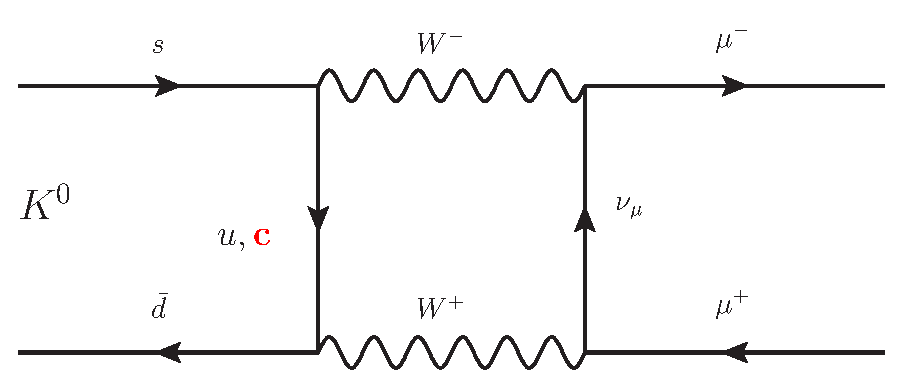
\includegraphics[width=0.6\textwidth]{Chapters/pQCD/GIM.pdf}
 \caption{The GIM mechanism in $K^{0}\to \mu\mu$ decay. Note the
   appearance of a charm quark contribution inside the box diagram.}
 \label{fig:GIM}
\end{center}
\end{figure}


For the next four years the charm quark existence was largely
overlooked. During the summer of 1974, Ting and his research team
started accumulating proton-proton data from the AGS at Brookhaven, hinting at the production of a new, very narrow
resonance of mass $\sim$ 3.1~GeV/$c^2$. Because of the very narrow aspect
the resonance had, it did not go into immediate publication. On
November 10, 1974, the team led by Richter who was operating the SPEAR
electron-positron collider at SLAC discovered that at beam energies
around E$_{b} \sim$ 
1.55 GeV, the counters went berserk. On November 11, 1974, both
collaborations at Stanford and Brookhaven announced their discoveries
of the \Jpsi~particle, which was quickly interpreted as a resonant
$c\bar{c}$ state, that is, a bound state of a charm quark and an anti-charm quark.

\begin{figure}[h]
\begin{center}
  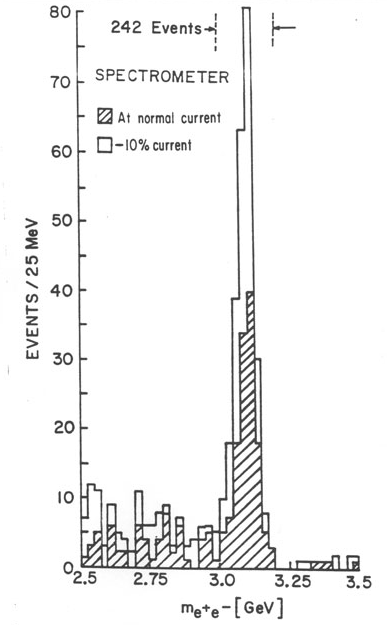
\includegraphics[width=0.25\textwidth]{Chapters/pQCD/psi_bnl.png}
  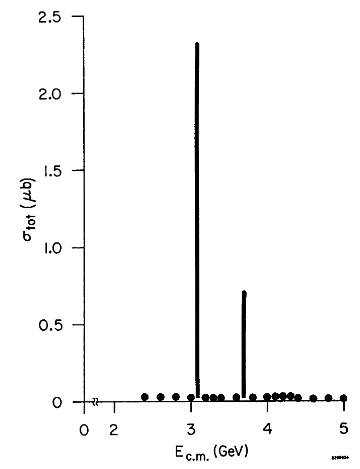
\includegraphics[width=0.3\textwidth]{Chapters/pQCD/psi_slac.png}
 \caption{First charmonium data. Left: statistics accumulated at
   BNL~\cite{psi_bnl}. Right: $e^{+}e^{-}$ events from SPEAR, showing a second
   resonance, the $\psi'$~\cite{psi_slac}.}
 \label{fig:psi}
\end{center}
\end{figure}

Two weeks later, in an energy scan for new particles in the charmonium
spectrum, excitement
struck again as the team at SPEAR discovers a second narrow resonance,
as can be seen in Figure~\ref{fig:psi}. One can see on the plot to the
right, events stacking at 3.1~GeV/$c^2$ and at 3.7~GeV/$c^2$, indicating the
presence of the $\psi'$. Only two years later, both Richter (SLAC) and
Ting (MIT) received the Nobel Prize in Physics ``for their pioneering
work in the discovery of a heavy elementary particle of a new kind''.

Shortly thereafter, the $\tau$ lepton was discovered at the SPEAR
facility~\cite{Agashe:2014kda}. This new lepton, discovered indirectly
through its weak
decay in $e^{+}e^{-}\to\tau^{+}\tau^{-}\to\mu^{\pm}e^{\mp}+2\nu$ came
first as an anomaly, before DESY confirmed the
signal. After establishing the quantum numbers of the newly-discovered
particle, it became clear that a new family of leptons was
released. With this discovery, the community soon concluded that two
additional quarks, $b$ and $t$ for bottom and top (or beauty and
truth) were to be expected. And indeed, in 1977, after seeing a hint
of a bump at $m \sim 9.6$~\unitMass\ prior to a significant upgrade, the
E288 collaboration (Lederman et al.) published their observation of
a new resonant structure in the di-lepton decay
channel~\cite{lederman}, which turned out to be the \PgU\ family, of particular interest for this thesis. 

\begin{figure}[h]
\begin{center}
  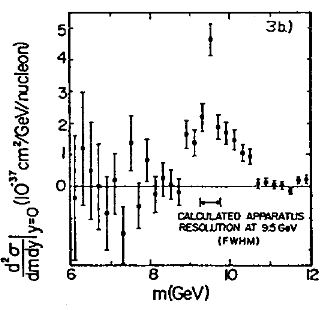
\includegraphics[width=0.5\textwidth]{Chapters/pQCD/first_ups.png}
 \caption{First bottomonium data, 1977. Dimuon events from proton-nucleus collisions
 at $E_{p}$ = 400 \GeV\ with the E288 experiment at Fermilab~\cite{lederman}.}
 \label{fig:upsi}
\end{center}
\end{figure}

\subsection{The discovery of the gluon}

% On the aftermath of the November revolution, there remained one grey
% area in the strong interactions. 
It is now clear that quarks exist
confined in the nucleons, and are probed only when increasing the
scattering energy enough so that the Compton wavelength of the
exchanged photon (in the case of DIS) is much smaller than the size of
the nucleon wavefunction. And doing so, we have seen in Equation~\ref{eqhalftheproton} that the
momentum fraction carried by the quarks was only
approximately half of the total available nucleon momentum. So it
seems clear that the colour field holding quarks in place is naturally
giving rise to other objects contributing to the nucleon integrity.


A recent account by Ellis~\cite{gluon_ellis} makes a very interesting
report of the events that led to think of strong interactions in term
a non-abelian $SU(3)$ theory. The first experimental signature
involving gluons in the final state was to be formulated in a 1976 paper by
Gaillard, Ellis and Ross, where they compute the gluon
bremsstrahlung\footnote{From the German word for ``deceleration radiation''.}
process in QCD~\cite{qqg} at $e^{+}e^{-}$ facilities, stating that it
should give rise to $q\bar{q}g$ final states. This final state is
observed experimentally in the form of three distinct clusters of
particles, further called~\textit{jets}.

\begin{figure}[t]
\begin{center}
  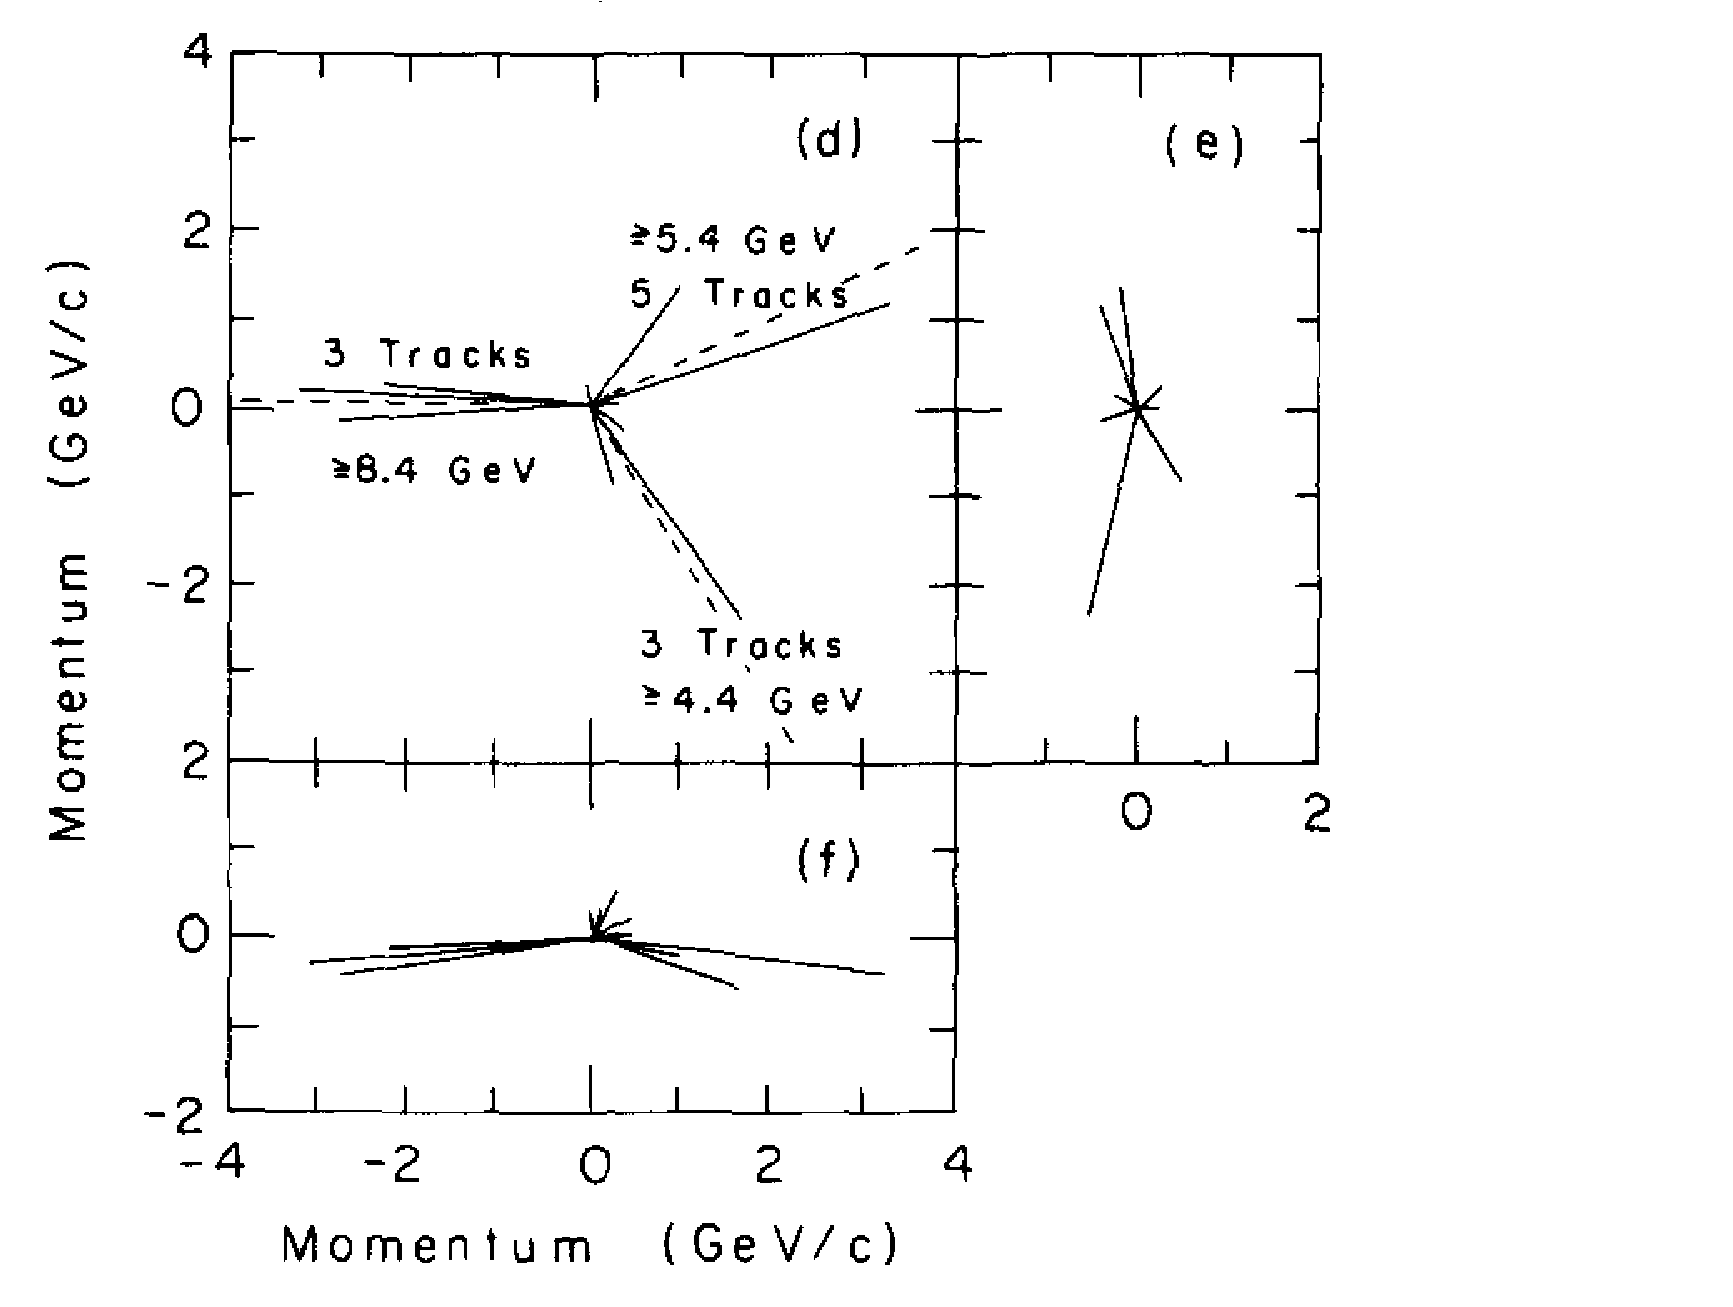
\includegraphics[width=0.7\textwidth]{Chapters/pQCD/qqg.png}
 \caption{A three-jet $q\bar{q}g$ event, from the TASSO collaboration \cite{wiik}.}
 \label{fig:gluonJet}
\end{center}
\end{figure}


Circumstantial evidence that gluons did exist was already
available. For example, charmonium and bottomonium decays to
three gluons, were computed to be the dominant decay mode for these
new objects. The discovery of the gluon radiation in 3-jet
events, and hence of its survival
to the long-distance process of hadronisation was announced jointly by
all four PETRA experiments at a Fermilab Lepton-Photon Symposium in
August 1979~\cite{tasso_g}. Figure~\ref{fig:gluonJet} shows one of the first such
$q\bar{q}g$ events recorded by the TASSO collaboration, where the three jets are easily seen in
the transverse plane (main panel).

This evidence for gluon bremsstrahlung is actually the basis for the
crucial QCD test described hereafter. 

\subsection{Testing QCD at \texorpdfstring{$e^{+}e^{-}$}{e+e-}, DIS
  and hadron colliders}
I will go briefly through several selected results from QCD analyses of
collider data from the eighties and nineties, which confirmed with
great accuracy many features of
\textit{perturbative}
% \footnote{A -- Non-perturbative effects require much
%   more computational power because of the many divergences. B --
%   Colour confinement should find a dynamical explanation, which is yet
% unknown.} 
QCD dynamics, as imposed by Equation~\ref{eq:qcdlagrangian}. 

\subsubsection{The non-Abelian nature of QCD}

The QCD Lagrangian discussed in Section~\ref{sec:lagrangian}, contains Feynman
diagrams with three-gluon and
four-gluons vertices. This is a specificity of the non-Abelian nature
of $SU(3)$, which has many consequences for the amplitude of various
processes. One example: 4-jet events in $e^{+}e^{-}$  collisions are
produced with tree-level QCD diagrams of Figure~\ref{fig:gluons}. Such
events will produce four clustered energy deposits (known as
\textit{jets}) in the final state, from which one can for example make
an event shape analysis.
\begin{figure}
\begin{center}
    \begin{subfigure}{0.244\textwidth}
      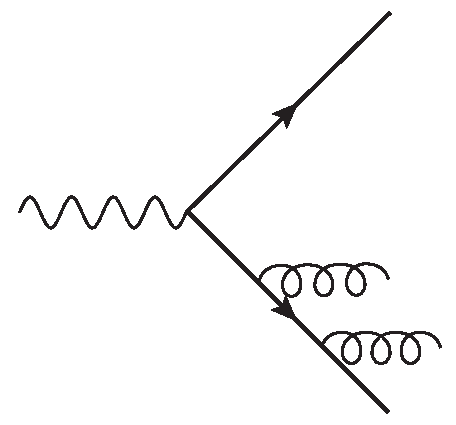
\includegraphics[width=\textwidth]{Chapters/pQCD/gluon1.pdf}\caption{}\end{subfigure}
    \begin{subfigure}{0.244\textwidth}
      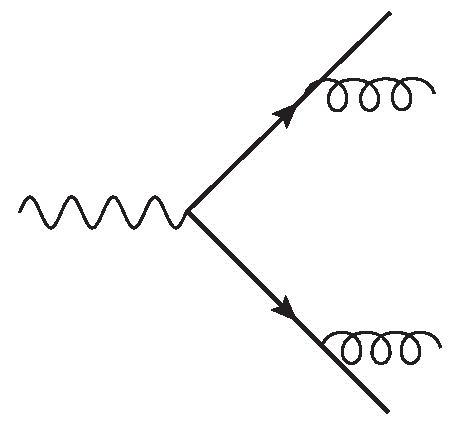
\includegraphics[width=\textwidth]{Chapters/pQCD/gluon2.pdf}\caption{}\end{subfigure}
    \begin{subfigure}{0.244\textwidth}
      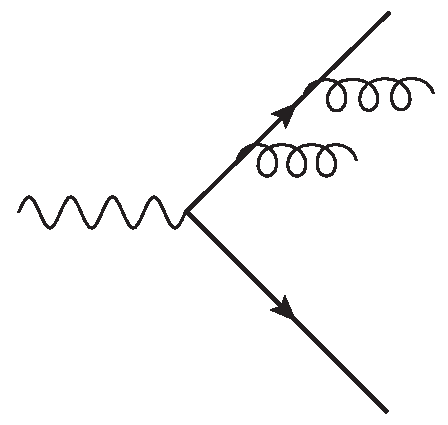
\includegraphics[width=\textwidth]{Chapters/pQCD/gluon3.pdf}\caption{}\end{subfigure}
\hfill ~\\
    \begin{subfigure}{0.244\textwidth}
      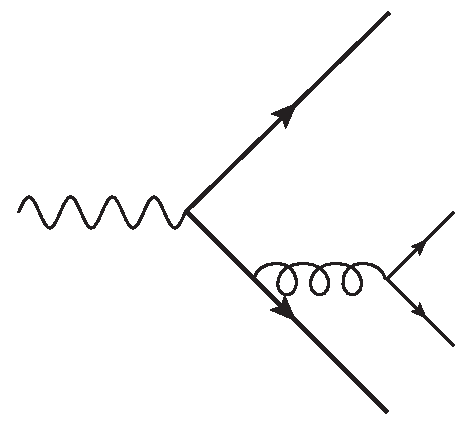
\includegraphics[width=\textwidth]{Chapters/pQCD/gluon5.pdf}\caption{}\end{subfigure}
    \begin{subfigure}{0.244\textwidth}
      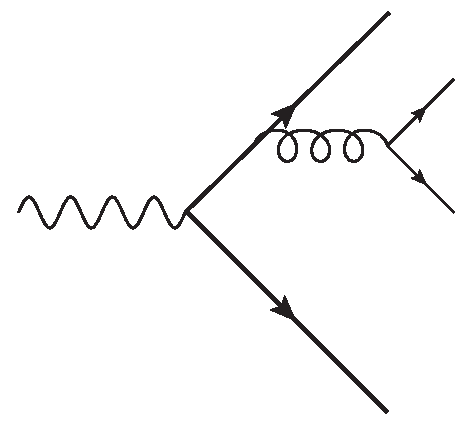
\includegraphics[width=\textwidth]{Chapters/pQCD/gluon6.pdf}\caption{}\end{subfigure}
    \begin{subfigure}{0.244\textwidth}
      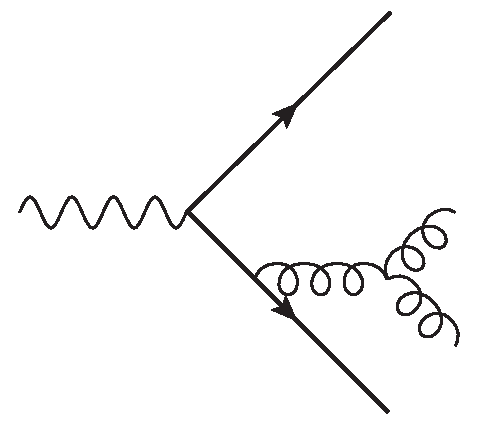
\includegraphics[width=\textwidth]{Chapters/pQCD/gluon7.pdf}\caption{}\end{subfigure}
    \begin{subfigure}{0.244\textwidth}
      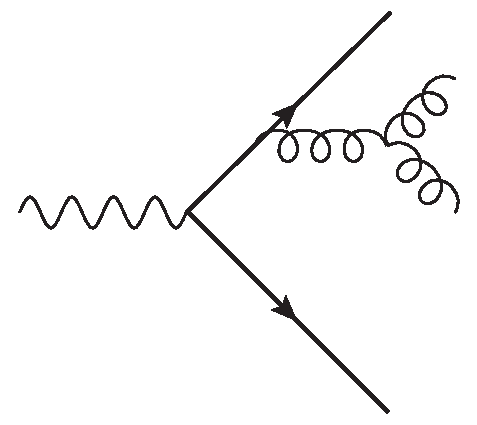
\includegraphics[width=\textwidth]{Chapters/pQCD/gluon8.pdf}\caption{}\end{subfigure}
    \caption{Tree-level Feynman diagrams for four jet events in electron
      positron collisions.}
    \label{fig:gluons}
\end{center}
\end{figure}


Take the four jet momenta ($p_1$, $p_2$, $p_{3}$, $p_4$) such that
they are energy ordered, $E_1 > E_2 > E_3 > E_4$. Most
likely the first two most energetic jets will come from the
quark lines, and one can define a plane $\mathcal{P}_{1,2}$. The question
is to know the angle between the plane $\mathcal{P}_{1,2}$ and the
plane delimited by the two sub-leading jets $p_3$ and $p_4$,
$\mathcal{P}_{3,4}$. First let me point out that double-bremsstrahlung diagrams (a), (b) and
(c) do not contribute very much to the correlation angle between
$\mathcal{P}_{1,2}$ and $\mathcal{P}_{3,4}$. 

Next, if gluon
radiation was like photon radiation in electromagnetism, i.e. Abelian,
then there would be no $g\to gg$ terms. There would then only be the
four-quark diagrams (d), (e). These would contribute as a
strong anticorrelation: Indeed, one can conclude from the gluon
polarisation that radiated gluons tend to be polarised in the plane
of the primary jets, and will split in two quarks of perpendicular
direction with respect to the $g$ polarisation. So diagrams (d), (e)
would give a wide angle between $\mathcal{P}_{1,2}$ and
$\mathcal{P}_{3,4}$. 

% Note that the colour factor for $g\to q\bar{q}$ is $C_{F}$ = 4/3 in QCD.

\begin{figure}
\begin{center}
  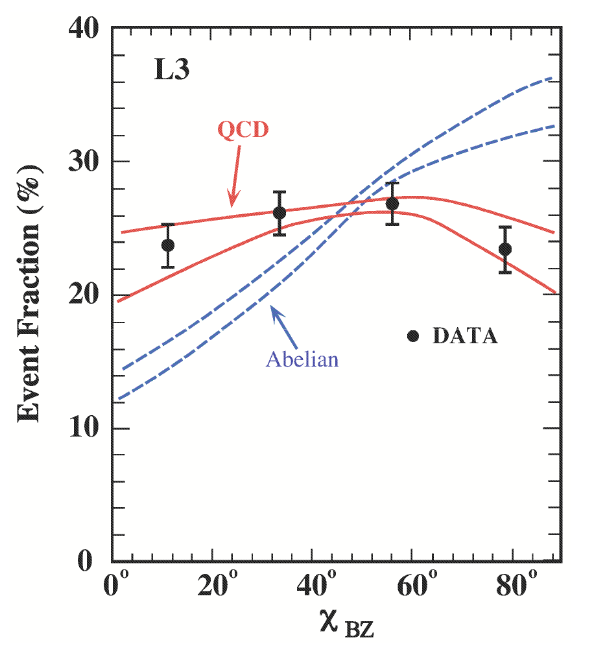
\includegraphics[width=0.5\textwidth]{Chapters/pQCD/xbz.png}
 \caption{The Bengtsson-Zerwas angle $\chi_{BZ}$ in four-jet events recorded by
   the L3 collaboration~\cite{xbz_l3}.}
 \label{fig:xbz}
\end{center}
\end{figure}


Finally, because of the non-Abelian nature of QCD, one has to consider
diagrams (f) and (g). It turns out that $g \to gg$ is dominant in QCD, by
virtue of the colour factor $N_{c}$ = 3, as well as the soft gluon
enhancement. Still using the
polarisation properties of gluon emission, the first gluon is radiated
along the plane $\mathcal{P}_{1,2}$, splitting in two gluons this time
mostly parallel to the polarisation. This correlation is weak but the
process is very abundant, resulting in a clear flattening of the
angular distribution in Figure~\ref{fig:xbz}. 

The angle $\chi_{BZ}$
used herein is called the Bengtsson-Zerwas angle~\cite{xbz}, defined by the
plane between the two leading jets and the two subleading jets. The
data from L3 collaboration is compared to a full-fledged QCD
simulation as well as to a straw-person model where
only Abelian terms are allowed. The Abelian theory curve is indeed peaking at
$\chi_{BZ} \sim \pi/2$, and does not match with the experimental data, indicating that the data does conform to
a non-Abelian theory.

Such four-jet analyses can be combined with other event shape analysis
and 3-jet events to yield a precise evaluation of QCD colour
factors. Figure~\ref{fig:combiLEP} presents a famous combination of results from LEP experiments (OPAL,
ALEPH, DELPHI) that shed light on the true value of QCD colour factors,
further confirming the $SU(3)$ group as its underlying theoretical structure.

\begin{figure}
\begin{center}
  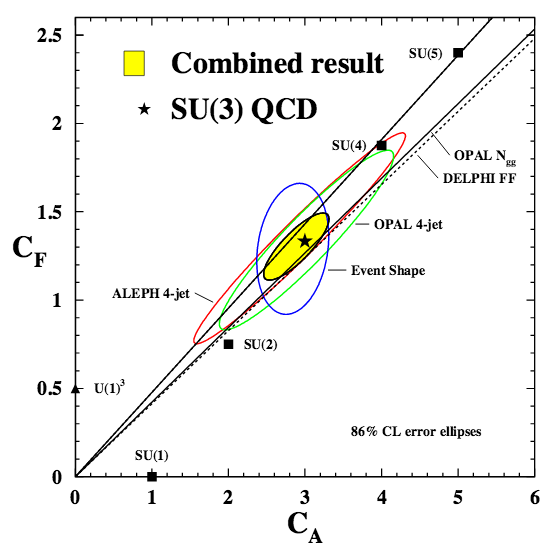
\includegraphics[width=0.5\textwidth]{Chapters/pQCD/combiLEP.png}
 \caption{The LEP-combined plot of $C_{A}$ and $C_{F}$. The yellow
   ellipsoid area is the combined uncertainty of the various jet and
   event shape measurements. Taken from~\cite{webber2}.}
 \label{fig:combiLEP}
\end{center}
\end{figure}

\subsubsection{Precision measurements of QCD effects}
Since the first attempt at measuring precisely $\alpha_{S}$ at the
time of PETRA and PEP colliders, many different processes from
$e^{+}e^{-}$ annihilation as well as lepton-hadron scattering gave
estimates of $\alpha_{S}$ with increasing precision. The total
hadronic cross section ratio $R$, the three-jet rate, event
shape observables, all yield experimental results on $\alpha_{S}$. It
may be worth noting that the JADE collaboration did find out a clear
experimental confirmation of the running of $\alpha_{S}$ in the rate
of three-jet events, already before the coupling constant value was
precise; back then, the data was compared to analytic QCD computations
at next-to-leading order in perturbation theory, including various
hadronisation models which performed relatively well, giving
$\alpha_{S}$ a mere 10\% precision~\cite{Bethke}.

The QCD programme at LEP, among other key results proving the
non-Abelian nature of QCD (cf. previous subsection) reduced
considerably these uncertainties, with $\mathcal{O}(\alpha_{S}^{3})$
precision observables: at the end of the LEP2 operation phase, the
world average was $\alpha_{S}(M_{Z})$ = 0.1184 $\pm$ 0.0031
(NNLO)~\cite{Kogler}.

Along came HERA (\textit{Hadron Elektron Ring Anlage}), at DESY in
Hamburg, with its two operation eras fully dedicated to lepton-hadron
scattering. Operating at $E_{e} = 27.5$ \GeV, and $E_{p} = (820, 920)$
\GeV, the HERA experiments (H1, ZEUS, HERMES) have accumulated, up to
2007, DIS data in an impressive phase space interval:
\begin{eqnarray*}
0.045 \: \textrm{GeV}^{2} <& Q^{2} &< 5.10^{5} \: \textrm{GeV}^{2}, \\
6. 10^{-7} <& x_{B} &< 0.65
\end{eqnarray*}

Capabilities of HERA experiments are very large: thanks to the
precise data accumulated in charged-current and neutral-current modes,
the QCD contributions to all processes, and the various parton PDFs can be computed
simultaneously. For example, inclusive jet cross section is measured
to the level of precision that one can see from ZEUS data in
Figure~\ref{fig:zeus} and compared to NLO QCD perturbation theory predictions. From that one
can extract for example $\alpha_{S}$, or measure the charm or bottom
quark mass with precision~\cite{H1Charm}. Figure~\ref{fig:zeus} (right) shows a
comparison of $\alpha_{S}$ from inclusive jets to NLO QCD
calculations, where the main sources of theory uncertainty come from
the various assumptions on either the perturbative part (DGLAP
evolution equations~\cite{Dokshitzer:1991wu}) or the PDF. 

\begin{figure}[htb]
\begin{center}
  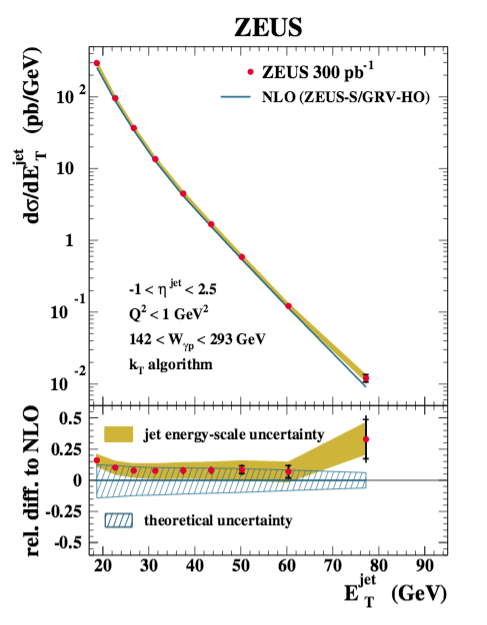
\includegraphics[width=0.35\textwidth]{Chapters/pQCD/zeus_jetCS.png}
  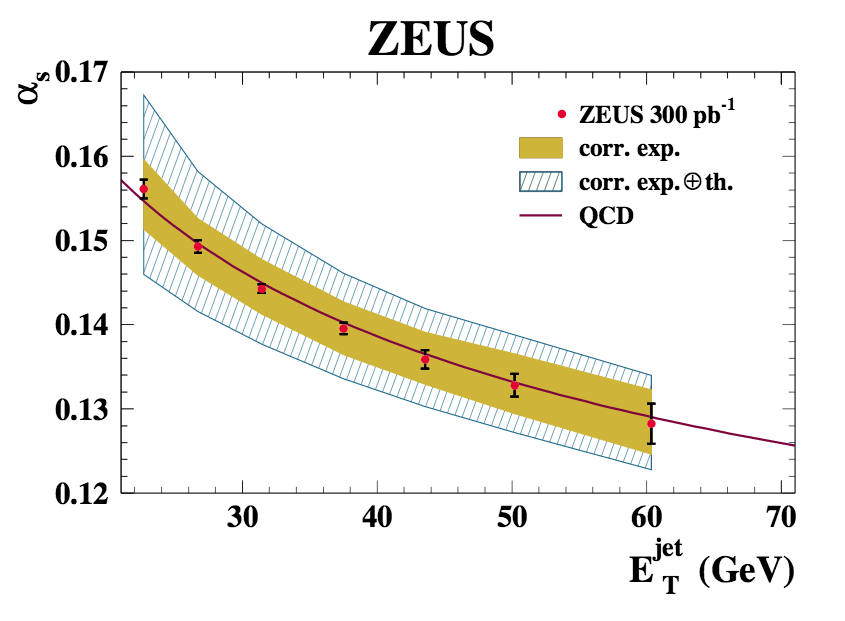
\includegraphics[width=0.63\textwidth]{Chapters/pQCD/alpha_s_zeus.png}
 \caption{Inclusive jet productions from the ZEUS collaboration. Left:
   the p$_{T}$ differential cross section. Right: $\alpha_{S}$. In both
   plots comparisons to dedicated NLO QCD calculations are shown. Taken from~\cite{Paul}.}
 \label{fig:zeus}
\end{center}
\end{figure}

This is only one small account of the various successes of QCD. In 2015, HERA experiments released a seminal paper
updating their long-collected parton PDF data~\cite{HERA_END}. One of the most
striking figures is reproduced as
Figure~\ref{fig:DIS_HERA}, where the quark and gluon PDFs are
reproduced at NNLO at a very close level of precision with fits
to data. This genuine piece of information will provide important
tuning to the study of hadron-hadron processes at LHC experiments. Indeed, almost all
processes (especially the most challenging ones, e.g. searches for Higgs
couplings to quarks) rely heavily on parametrising the momentum fraction carried by
gluons and quarks in the proton. For heavy quarkonia this also plays a
role, as gluon fusion is the dominant process at
LHC energies.

\begin{figure}[htb]
\begin{center}
  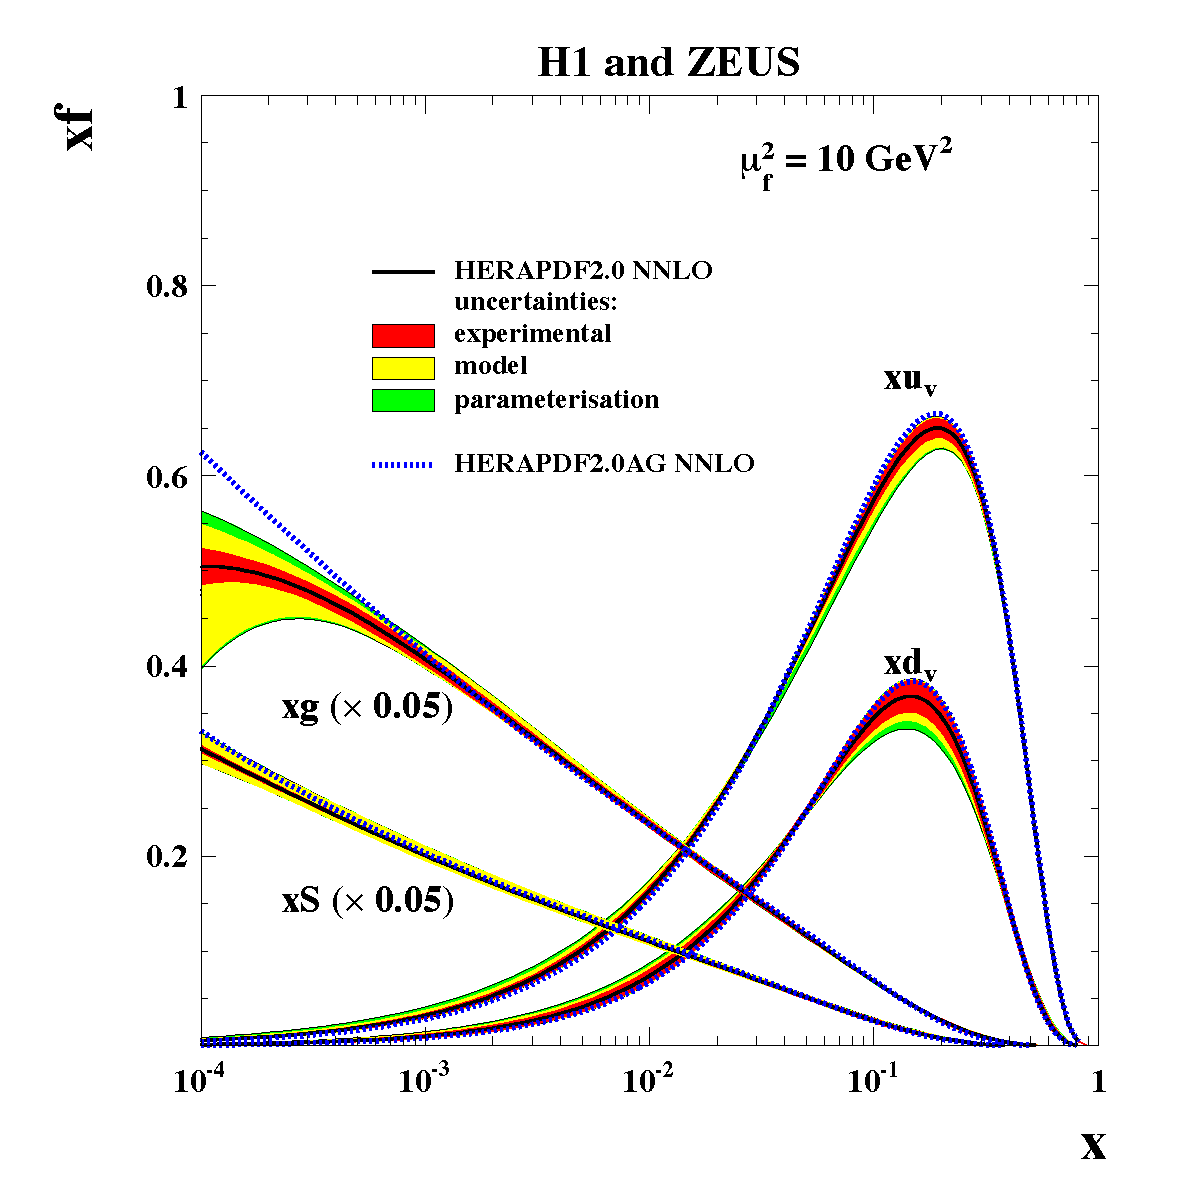
\includegraphics[width=0.65\textwidth]{Chapters/pQCD/DIS_HERA.pdf}
 \caption{Parton distribution functions $xu_v$, $xd_v$, $xS =
   2x(\bar{U}+\bar{D})$ and $xg$ of HERAPDF2.0 NNLO at $\mu_{\rm f}$ =
   10 GeV$^{2}$~\cite{HERA_END}. Gluon and sea distributions are scaled down by a
   factor of 20.}
 \label{fig:DIS_HERA}
\end{center}
\end{figure}

% \vfill\newpage

\subsubsection{Modern running coupling constant measurements}
\label{sec:alphasrunning}

Finally, the best illustration of QCD success is the comparison of its
predicted running of $\alpha_S$ with experimental measurements related
to this quantity, at various orders of perturbation theory. This is
presented in Figure~\ref{fig:alphasrunning},
from~\cite{Agashe:2014kda}. Nowadays, the running of $\alpha_S$ is
well understood, and is of prime importance for a large majority of
Standard Model physics analyses. Indeed, almost every rare physics
process studied at the LHC is usually extracted from the sum of several
templates of signals whose cross section is known to
several orders of the strong coupling constant. The precise knowledge
of QCD is crucial also in the modelling of~\textit{hadronisation},
which is the process by which final state particles radiate softer
particles and form detectable jets.

\begin{figure}[h]
\begin{center}
  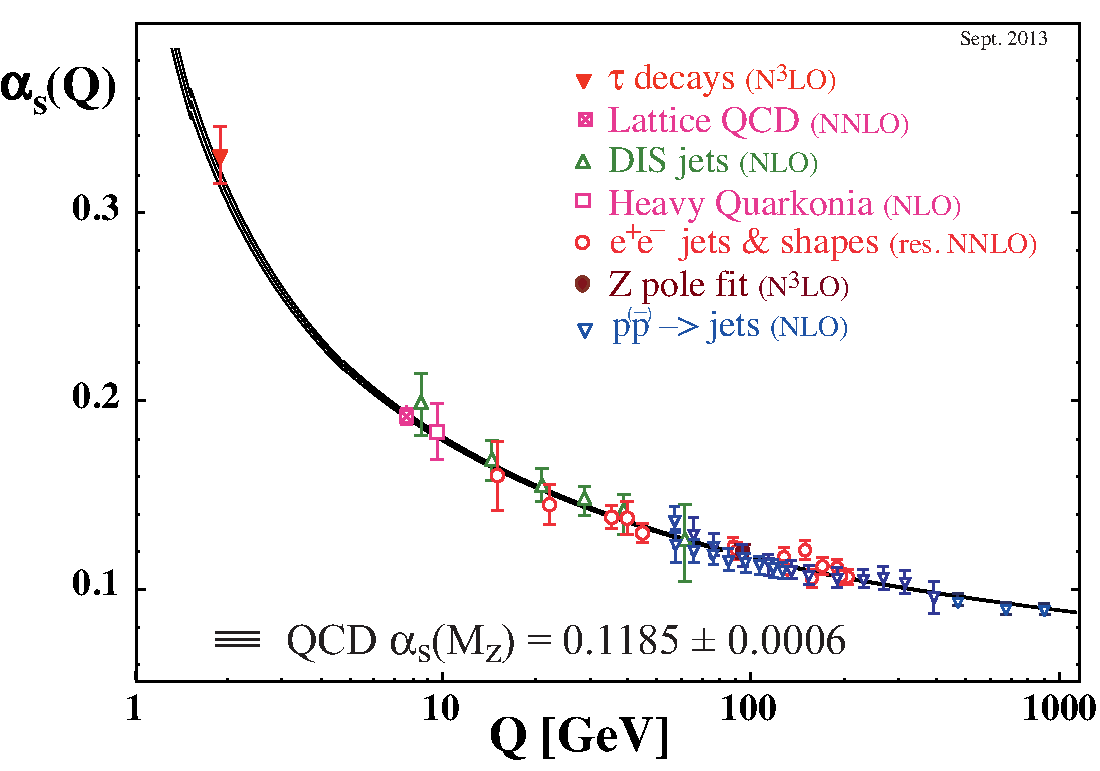
\includegraphics[width=0.8\textwidth]{Chapters/pQCD/asq-2013.pdf}
 \caption{The running of the coupling constant of QCD~\cite{Agashe:2014kda}.}
 \label{fig:alphasrunning}
\end{center}
\end{figure}

 % The running of the coupling constant, which I have
% tried to detail down to the renormalisation group equation, gives a dynamical
% reason for quark confinement, and that is a unique aspect of QCD.
% The fact that
% there are three colour charges, and that force carriers may interact
% together, is a specificity of QCD. Of course
% all non-Abelian theories have a self-coupling for gauge
% fields, but in the particular case of QCD, the gauge fields are
% massless and this interaction plays an enormous role, starting from
% relatively low energies. 

\vspace{0.5em}
\begin{center}
  \fbox{
    \parbox{0.9\textwidth}
    {\textsf {In this section I have presented how the quantum theory for
        quarks and gluons came to be constructed, and to show some of its
        basic properties. \\ One of the key open questions of QCD is colour
        confinement. What actually drives the colour charges to equilibrate
        together and cancel themselves in the final state? What are
        the thermodynamical properties of a many-body system of colour
        degrees of freedom ?  % happens when one simulates such a system of 
        % massive and massless objects exchanging the colour quantum numbers,
        % one turns up the temperature and increases the pressure on the system?
        % What happens when the charges are getting closer and closer to each
        % other
        ? What experimental
        possibilities are available today to assess these questions? That is
        what the next section is about.
      }}} 
\end{center}

\clearpage

\section{From confinement to deconfinement}

\subsection{Phase transition at finite temperature}

Contemporary to the quark model is the discovery of microwave
background. The idea had peered through that the universe \textit{cooled down} to the T$\sim 3K$ measured in 1965,
providing evidence for a hot primordial universe. At the same time,
people studying nuclear interaction in high-energy collisions were
trying to predict the particle yields in a self-consistent
way. Hagedorn's hypothesis~\cite{Hagedorn} is worth mentioning at this point, since it
connects directly with the deconfinement sought in current day
high-energy nuclear interactions. His statistical bootstrap model
suggests that the density of hadronic states as a function of their
mass, $\rho(m)$, must be
asymptotically equivalent to the particle yields, $\sigma(E)$:

\begin{equation}
log(\rho(m)) = log(\sigma(E))
\end{equation}

Indeed, Hagedorn went on to conjecture a set of equations for
$\rho(m)$ and $\sigma(E)$ that would satisfy this criterion. In the
asymptotic limit, it translates into a density of available states which
increases exponentially with the mass:
\begin{equation}
\rho(m) \approx e^{\frac{m}{T_{H}}}
\end{equation}

and $T_{H}$ is called the Hagedorn temperature, of a value around 170 MeV. At
this temperature, the partition function becomes singular. It was
deduced that in a hot Big Bang model, the universe did produce a
wealth of unstable particles which eventually cooled down, but with
Hagedorn's temperature one could foresee that about 10 microseconds
after the Big Bang, the temperature of the universe was around 170
MeV.

In 1975, Cabibbo and Parisi~\cite{cabipari} suggested that the exponential decrease in
spectrum ($\sigma(E)$) is in fact connected to the existence of a
deconfined phase for quarks, transition that was thought to
occur at $T_{H} \sim$ 170 MeV.

So the immediate question comes along: Can we recreate this in laboratory
conditions, using ultrarelativistic nuclear beams? It should be
possible to ramp up the energy of the beams and collide enough
hadronic matter in a small volume as to increase the density and
eventually probe the existence (or absence) of this deconfinement
transition.

\begin{figure}[h]
\begin{center}
  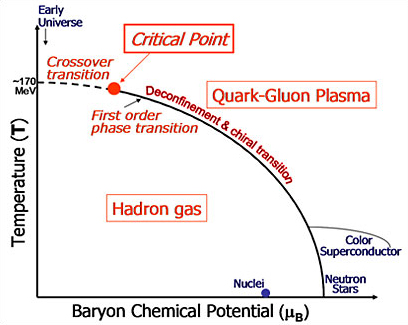
\includegraphics[width=0.8\textwidth]{Chapters/pQCD/phase.jpg}
 \caption{A schematic approach to the QCD phase transition.}
 \label{fig:transition}
\end{center}
\end{figure}

Figure~\ref{fig:transition} shows how the temperature and the baryon
chemical potential $\mu_{B}$ are related in the current picture of the phase
diagram. 

The study of the QCD phase transition with calculations on the lattice
helped drawing the thermal properties of a strongly interacting set of
objects (fermions and/or bosons) enduring increasing temperature and
pressure. For pure gluonic matter for example, the equation of state
from~\cite{lattice_g} shows a rapid approach toward an ideal gas
behaviour.
Increasing computational power helped increasing the complexity of
lattice simulations. Eventually, the energy-density/temperature
profile of models including two or three degenerate flavours of quarks
was computed and compared to what experiments were able to
perform. Figure~\ref{fig:tc_lattice} from~\cite{Karsch:2001cy} shows
such a comparison, where we 
see that the transition temperature is at T$_{c} = (173 \pm 15)$ MeV
for two quark flavours, and is accessible at the Super Proton
Synchroton (SPS) at CERN as well as at the
Relativistic Heavy Ion Collider (RHIC) at Brookhaven National
Laboratory (BNL).


\begin{figure}[h]
\begin{center}
  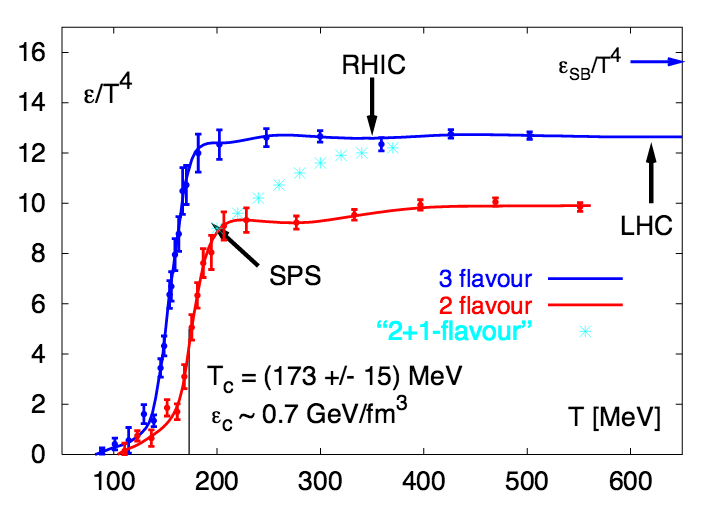
\includegraphics[width=0.8\textwidth]{Chapters/pQCD/phase_tc.png}
 \caption{Lattice calculations of the energy density as a function of
   lattice temperature, from~\cite{Karsch:2001cy}.}
 \label{fig:tc_lattice}
\end{center}
\end{figure}

There are currently two laboratories able to put the conditions
together to study the phase transition. At BNL,
RHIC collides protons, deuterons, gold nuclei, and more. For
gold-gold collisions, the energy in the centre of mass reaches
\snn\ = 200 \GeV. At CERN, fixed target experiments near the
SPS reached a \snn\ $\approx$ 17 \GeV, while
the LHC can provide lead beams to CMS, ALICE, ATLAS, and LHCb
detectors, reaching a \snn\ = 5.1~TeV in PbPb collisions\footnote{As I write this, these collisions have not yet started but correspond to the 13~TeV pp collisions that are currently ongoing.}.

If the thermal behaviour of nuclear matter under extreme pressure and
density can be studied, one can wonder what is the time evolution of
the hot medium produced. % of
% the experimental conditions
 Indeed, the deconfined phase sets
in progressively% when the strange quark mass is relatively high
% compared to the two other light quarks
\footnote{This is a \textit{crossover} instead
of a phase transition.}. In Figure~\ref{fig:timescales} the
timescales of the various processes thought to occur in
ultrarelativistic heavy ion collisions are layed out.

\begin{figure}
\begin{center}
  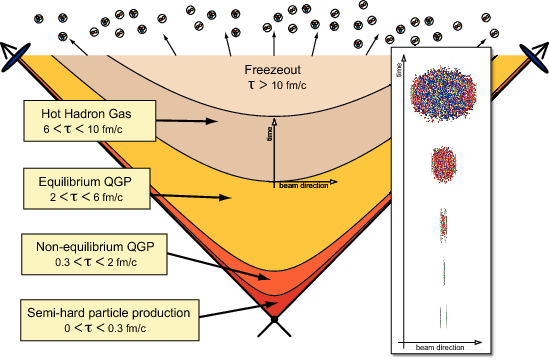
\includegraphics[width=0.75\textwidth]{Chapters/pQCD/timescales.png}
 \caption{A time frame cartoon for the thermodynamics of the QGP in
   heavy ion collisions. Both
   diagonals represent the light-cone projection of incident
   beams. The overlay on the right shows the evolution in the
   laboratory frame. From~\cite{strickland_phase}.}
 \label{fig:timescales}
\end{center}
\end{figure}


% I am getting closer to the main questions that my analysis topic is
% aiming at.
I have asserted that colliders such as LHC and RHIC should be
able to produce a deconfined phase of QCD, known as the Quark-Gluon
Plasma (QGP). Now we should try to find out what are the properties of
the 'little bang' produced in laboratory, and how can we build
strategies to probe this little bang efficiently? Finally, how can
experimental observation be related to the predicted transition?

\subsection{Measuring the properties of the quark-gluon plasma}

In DIS experiments, physicists have been able to identify and %  speculate and deduce from
% colourless 
probe the distribution of point-like objects and the force
binding them together inside the nucleons. In a way, experimental
heavy ion collisions can follow the same strategy. If we were able to
use as a probe, one object not interacting strongly with nuclear matter,
then it should be possible to use the alteration of
the probe passing through to extract physics on the created medium. I am intentionally using loose terms.
For now, let us set some rules:
\begin{itemize}
\item[1] I do not know beforehand what to expect from colliding nuclei, from
  textbook, that are mostly dealing with zero temperature particle physics;%  to Kennedy Jr.'s plane being absorbed into a
  % black hole, simply because the phenomenology detailed above could be wrong
  
\item[2] I anticipate that some probes may be
  very altered, some less. We would be interested in the spectrum of each
 type of probe, passing through whatever was created, as much as 
  in their normalisation: their total yield can carry information about the phase they traversed;
\item[3] I can however anticipate that if my experimental settings
  reach the deconfinement transition, effects on some probes would be very clear: I need a baseline for whatever would happen before
  the transition. This is crucial if my transition is continuous, from
  vacuum QCD to above the critical density.
\item[4] Finally, I need to get an experimental handle on an effective
  'temperature', a measure of the violence of the collision.
\end{itemize}
 
% The phase diagram tells us that the transition from low to high
% temperatures will make nuclear matter go through a stage where it
% resembles a ``hadron gas'' for some time. A probe could be affected,
% but on the principles that QCD should still work, I can work out some
% model for this.
When colliding nuclei at very-high velocities, the relativistic
contraction of length scales plays a role: the crossing time $\Delta t$ for nuclei can
be estimated as:

\begin{equation}
t \sim \frac{d}{c} \Longrightarrow \Delta t \approx
\frac{2R_{o}/\gamma}{c}.
\end{equation}

Taking 10 fm as an order of magnitude for the nucleus radius $R_{o}$,
and using the energies at which the LHC operated for the lead-lead scheme,
$E_{Pb}$ = 1.38 $A$ \TeV, we have the Lorentz factor $\gamma$ = 1380
and the crossing time for lead nuclei at LHC energies is $\Delta t
\approx 10^{-2}$ fm$/c$. This can be compared to the timescale
of strong interactions,
\begin{equation}
t_{QCD} \sim \frac{1}{\Lambda_{QCD}} \approx 1 \textrm{fm}/c
\Longrightarrow \Delta t \ll t_{QCD}
\end{equation}
As a consequence, any effects related to particle production via
strong interactions will occur well after the nuclei have crossed.

There comes a big difference with DIS experiments: one has to produce
the probe just before the QGP is formed because it does not last for
long. The cartoon in Figure~\ref{fig:timescales} informed on
% us that from the equation of state, one can infer 
the lifetime of the QGP: the kinetic freeze-out occurs around
10~fm$/c$. It would be hopeless to try to shoot something at a QGP
that lasts for less than 10~fm$/c$.

What objects can be produced in the high-energy nuclear collision
early enough to see the rise and fall of the deconfined phase? Hard
(high-$Q^{2}$)
particle production, including photons and weak bosons that should not be sensitive to the strongly interacting medium. In this sense, the large
energy carried by jets would be good a candidate, as they should see a lot
of the QGP on their way out towards the detector. Heavy quarks would
also be good candidates, 
% as their spectrum can be well measured, and
provided that the initial process was hard enough (say, above 1 GeV).
% one could measure the modification of their spectrum or angular distribution. 

\begin{figure}[h]
\begin{center}
  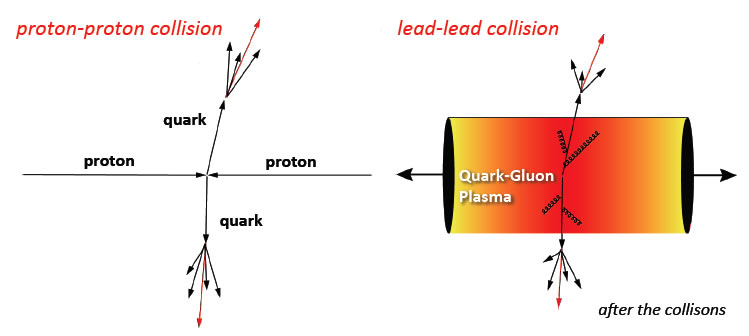
\includegraphics[width=0.7\textwidth]{Chapters/pQCD/collisions.jpg}
 \caption{A schematic approach to a hard partonic interaction in
   (left) a proton-proton interaction and (right) a coloured medium.}
 \label{fig:collision}
\end{center}
\end{figure}


Figure~\ref{fig:collision} is here to give a schematic idea of what
happens in the case of the production of two quark jets. Both quarks
are emitted back to back in the initial parton reference frame. If
they are produced close to the QGP boundary, it is likely that one
will escape, while the second one will scatter and interact
strongly with most of the medium, changing significantly the topology:
the away side is completely absorbed, as measured by the STAR
collaboration in gold-gold (AuAu) collisions~\cite{starquenching}, and
presented in Figure~\ref{fig:jet_star}.
\begin{figure}[h]
\begin{center}
  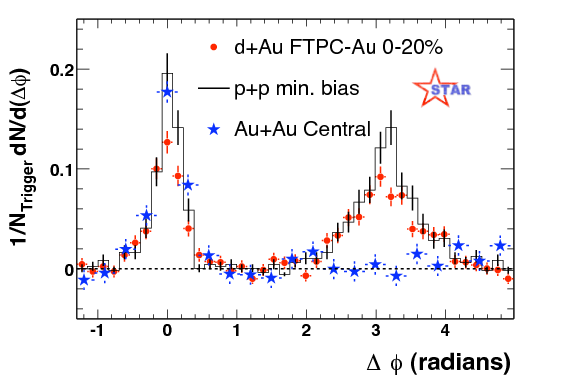
\includegraphics[width=0.7\textwidth]{Chapters/pQCD/jetstar.png}
 \caption{Azimuthal di-hadron correlations in pp (black histogram), dAu (red circles) and AuAu (blue stars) collisions from the STAR collaboration.}
 \label{fig:jet_star}
\end{center}
\end{figure}



On the figure one can see that away-side jets are also slightly modified in
deuteron-gold (dAu) collisions~\cite{starquenching}, indicating some interaction with
non-QGP nuclear matter. Indeed, one does not expect to match the
conditions for a hot medium formation when a very light nucleus (such
as a deuteron) hits a much heavier one. This constitutes a measurement of
nuclear matter effects.

This immediately raises the question of the 'violence' of the QGP
phenomenon. The impact parameter not being measurable, one has to rely
on a model to estimate the \textit{centrality} of the collision.
In various Since the early heavy ion experiments of the seventies and eighties,
the charged hadron multiplicity has been measured to increase
as a function of log $\sqrt{\snn}$, as is shown on Figure~\ref{fig:pbpbmult}. 

\begin{figure}[h]
\begin{center}
  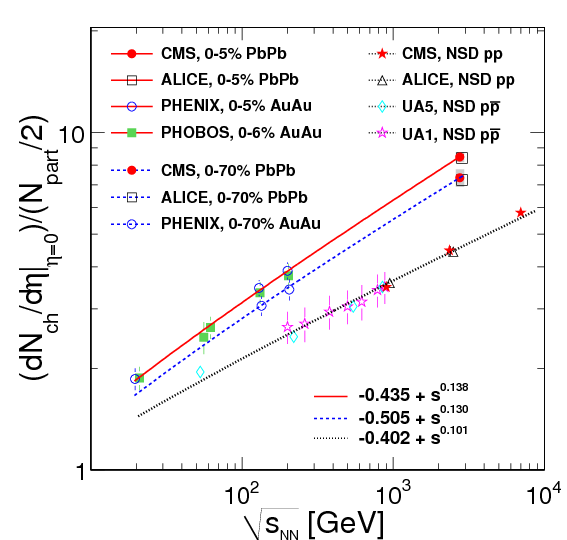
\includegraphics[width=0.6\textwidth]{Chapters/pQCD/multhi.png}
 \caption{Charged hadron multiplicity in proton-proton and heavy ion
   collisions~\cite{pbpbmult}.}
 \label{fig:pbpbmult}
\end{center}
\end{figure}


One
can see that this log $\sqrt{\snn}$ dependence also applies to central
heavy ion collisions. The plot shows that for the most central values, the charged
particle yield changes, as well as the slope, indicating a
classification of events as a function of global event variables works
well. Nowadays the events are cut in percentiles of increasing centrality,
that are directly correlated to the charged hadron multiplicity in the
event or the sum of energy deposits in the forward directions of the
detector.


This short review of possibilities led me to
present the centrality of the collisions, as well as the (p-A or d-A)
baseline for cold nuclear matter effects. This anticipated a
discussion of global event variables which are relevant for any
heavy ion measurement.
In Section~\ref{sec:centrality} I shall present in more detail how
these experimental handles correlate with the assumed number of
nucleons participating in the collisions, as well as with the number
of hard scatterings, both derived from a Glauber model calculation~\cite{Glauber:1970jm}.
% \begin{figure}[h]
% \begin{center}
%   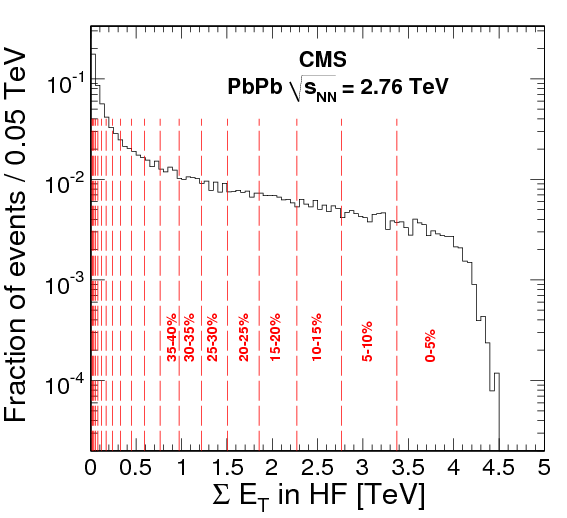
\includegraphics[width=0.6\textwidth]{Chapters/pQCD/centralitybins.png}
%   \includegraphics[width=0.6\textwidth]{Chapters/pQCD/npartncoll.png}
%  \caption{Charged hadron multiplicity in proton-proton and heavy ion collisions}
%  \label{fig:pbpbmult}
% \end{center}
% \end{figure}

Finally, bound states of heavy quarks should play a 
central role in measuring the thermal properties as they also come
from a hard process. Furthermore, the spectroscopy of quarkonia
is such that one family (charmonium or bottomonium) has members with
increasing sizes or binding energy, with different radial and/or orbital quantum numbers. It turns out that
in the most simple considerations, the energy levels computed are of
the order of the deconfinement temperature, or of small integer
multiples of T$_{c}$. This means that \Jpsi, $\psi(2S)$,
\PgU(1S,2S,3S) may react differently to the quark-gluon heat. This is
covered in the next section, in a larger detail.

% All this goes in the positive direction of being able to measure the
% existence of deconfinement in high-energy nuclear reactions. When
% colliding nuclei however, we do not know beforehand if all collisions
% produce a QGP. We can speculate that this depends on the impact
% parameter of each collisions. This is especially important when we
% consider that the geometry of the collision is 
\subsection{Sequential melting}

% Let us take a step back and recall the consequences of asymptotic freedom. As $Q^{2}$
% increases, the coupling decreases, and I have mentioned in Section~\ref{sec:running} that in
% QCD this is due to the existence of gluon self interactions.
%  Probing a colour charge with increasing resolution, one will start to resolve
% more vacuum fluctuations, and by virtue of the colour factors, the
% gluon self couplings play a higher role. In turn, the colour charge
% that one is trying to probe gets \textit{antiscreened} by the gluon
% fields popping out of vacuum.


As seen in Section~\ref{sec:november}, the quarkonium states of the
charmonium family and of the bottomonium family are heavy quark resonances, i.e. a
bound state of heavy quark ($c$ or $b$) and a heavy anti-quark of the
same flavour ($\bar{c}$ or $\bar{b}$, respectively).

Each family has its own spectroscopy, meaning that one can observe
several energy levels of this resonant structure. For example, in the
case of charmonium, the \Jpsi represents the fundamental level of
$c\bar{c}$ states with a spin-parity combination J$^{P}$ =
1$^{-}$. The $\psi(2S)$ state often called ``psi-prime'', is the first radial
excitation of this level. There are other states in the charmonium
family as we shall see in Chapter~\ref{chap:pquarkonia}.


%When thinking about bound states and their radial energy levels, one
%can think about the hydrogen atom, and anticipate that
%higher energy excitations have, as in the Bohr picture, larger radii as
%$n$ increases. Strictly speaking I am not certain how far the analogy
%can be taken, since the hydrogen atom energy levels are function of
%the reduced mass $\mu$ = $m_{p}m_{e}$/$(m_{p}+m_{e})$. Hence in a system
%of two heavy quarks of equal mass, I fear the two-body problem could not be
%easily reduced to a central interaction. But at least the reasoning in
%terms of interaction lengths should hold: a higher energy level seems
%to correspond a wider system.


When studying the effects of the QGP on heavy quark resonances, Matsui
and Satz have found in 1986~\cite{melting} that considering a
non-relativistic interaction potential for two heavy quarks $Q$ and
$\bar{Q}$,
\begin{equation}
\label{eq:potential}
V(r) = \sigma r - \frac{\alpha_{\rm{Coul.}}}{r},
\end{equation}
the string tension $\sigma$ depends on the temperature $T$. For an
isolated system (meaning $T=0$) of charm quarks (let us take for instance the \Jpsi), %they enounce 
we can take $\sigma \approx 1~\GeV/ \textrm{fm}$,
and $\alpha_{\rm{Coul.}} \approx$ 0.5 for the effective Coulomb
interaction coupling. Solving the radial energy equation they get a
\Jpsi radius at zero temperature of

\begin{equation}
E_{\Jpsi} = 3.1 \; \GeV, m_{c} =  1.56 \; \GeV \Longrightarrow r_{\Jpsi} \approx 0.25 \; \,\textrm{fm}.
\end{equation}


The colour screening evolution towards and above QGP transition
temperatures had been studied previously in~\cite{DeGrand}. For a
quark/anti-quark pair, the relevant quantity accounting for a 'size'
is the correlation function $\Gamma_{q\bar{q}}(r,T)$, with $r$ being
the static system's radius, and $T$ the temperature of the gluonic
bath\footnote{At that time, full SU(3) gluons + quarks lattice
  simulation were not available yet.}. From lattice simulations one
can observe the correlation length decreasing steadily when the
temperature passes $T\sim 200$ \MeV. Matsui and Satz identify this with
the binding string tension decreasing with $T$, arguing that at the
deconfinement temperature, $\sigma(T_{c}) = 0$. Above deconfinement
a colour-screened version of the Coulombic potential persists, from
which one can expect dissociation of the quarkonium states at definite
temperature values. In this picture, % speaking of $T_{\rm{diss}}$ or
% energy density is equivalent, and
the resulting physical outcome is a sequential reduction of the overall charmonium yield with increasing
of the energy density created in the collision. 


\begin{figure}[h]
\begin{center}
  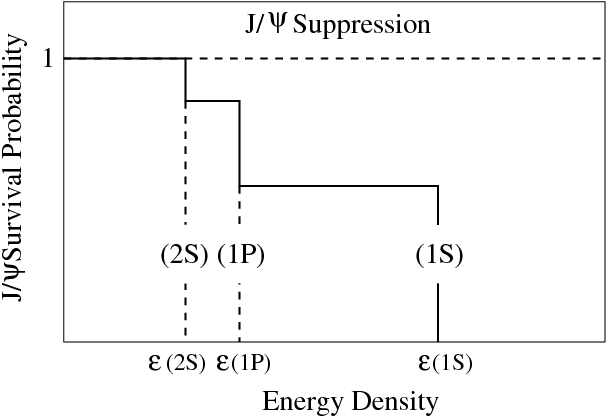
\includegraphics[width=0.5\textwidth]{Chapters/pQCD/seq-charm.png}
  \\ \vspace{1cm}
  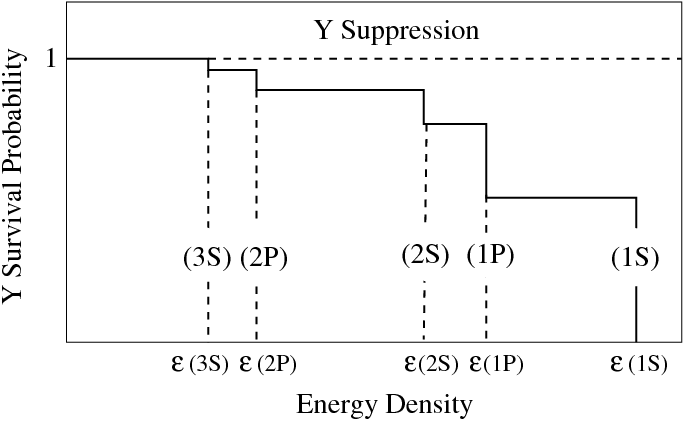
\includegraphics[width=0.5\textwidth]{Chapters/pQCD/seq-bottom.png}
 \caption{A schematic approach to sequential melting of quarkonium
   ground states as a function of energy density. Top: the \Jpsi
   suppression sequence. Bottom: the \PgUa~suppression sequence.}
 \label{fig:sequential}
\end{center}
\end{figure}
\newpage
This is often called a
\textit{sequential melting} scenario, which resembles the rough sketch depicted
in Figure~\ref{fig:sequential}. One can see that the bottomonium
family is slightly more complicated than the charmonium family. I
will elaborate more on the spectroscopies of each family in the next
Chapter. Finally, the height of each step in
Figure~\ref{fig:sequential} is driven by the spectroscopy of each
quarkonium family, where de-excitations from excited levels populate the
lower-lying states.% , and each de-excitation can be assigned a feed-down
% fraction, or probability.


\vspace{0.5em}
\begin{center}
  \fbox{
    \parbox{0.9\textwidth}
    {\textsf {This marks the end of Chapter 1. I have presented how QCD came
together and imposed itself as the theory for strong interactions
between quarks and gluons. I have briefly presented some aspects of what
makes QCD special, and some connections with ultrarelativistic nuclear
collisons in experiments. I have also presented how some observables are
relevant to estimate the effect of the QGP, either in an alteration of
their spectrum, or of their production rate. In the next Chapter I
will concentrate on the case of quarkonia: How do we understand the
production in vacuum of such extended objects, and how we explain
their observed modification in nuclear matter. }}} 
\end{center}



% - Plot de transition de phase QCD ( epsilon/T$^4$ vs T) -> Tc 

% Conclure soit sur une petite liste des signatures (bof), soit sur la mention de Matsui et Satz

% (très facilement connectable avec la température que tu viens d'introduire). 

% Bonus : si t'as envie de mentionner LA mesure de température. 


\chapter{Aspects of quarkonium physics}
\label{chap:pquarkonia}

\minitoc

\myepigraph{At least we can all agree on one thing: The people who see
  the dress as white are utterly, completely wrong.}{Adam Rogers, in \textit{The Science of Why No One Agrees on the Color of This Dress},
  www.wired.com}


\section{Quarkonium production in vacuum}
\label{sec:production}
% Because of several factors, the quarkonium production is a
% long-standing riddle.
Quarkonia were first studied extensively at
$e^{+}e^{-}$ colliders. For example, the BABAR detector at Stanford (USA)
and BELLE at Tsukuba (Japan) have analysed hundreds of inverse
femtobarns of $e^{+}e^{-}$ events at the centre-of-mass energy of
a $\Upsilon(4S)$ at rest (and above), to study $B$ meson production and other
heavy flavour related processes. Among these, the spectroscopy of
heavy flavour and quarkonia has been studied with great
precision~\cite{nora}.
%  In this Section, I will
% prevent myself from saying that no-one is able to understand
% quarkonium production (there \textit{is} hope).
The quarkonium production mechanisms are however, still debated.
 I will start with a
discussion of the allowed decay processes for quarkonia, by virtue of
the Okubo-Zweig-Iizuka (OZI) rule~\cite{Okubo:1963fa,Iizuka:1966fk,Zweig:570209}; this will
help me to give a naive view of the possible production modes, by
simply turning around the decay process. Then, I will discuss what
the binding of two quarks means in terms of
spectroscopy and decay, before moving to an experimental review of
some interesting results, and finish with an increase in temperature to
see to what risks a quarkonium exposes itself when wandering in nuclear
matter. Beginning with an experimental review, I will make a detour in
charmonium physics, before moving to a discussion of available results in
the bottomonium sector.


\subsection{Introductory remarks: the OZI rule}
\label{sec:OZI}
In Chapter~\ref{chap:pqcd}, I have mentioned the existence of new
resonances in the 1970's dilepton spectrum of $e^{+}e^{-}$
colliders. One of the particularities of these new \Jpsi and $\Upsilon$ peaks
is their very narrow signal shape, compared to what was usually known in the
lower part of the mass spectrum (except for the $\phi$ meson, which is
$s\bar{s}$). 
\\
This is a consequence of the OZI
rule. For heavy quark-antiquark states $\psi$ of the same flavour $s\bar{s},\,
c\bar{c},\, b\bar{b}$, the possible decay processes are: electromagnetic
annihilation or hadronic decays. The rate of the electromagnetic
annihilation quarkonium is of a typical order
$\alpha_{QED}^{2}$~\cite{gatto}. On the other hand, the hadronic 
decay is mediated by the strong interaction. So at first, one can say
that quarkonia will either decay strongly via the hadronic channel, or
via QED-mediated processes, seemingly with a smaller rate (as
$\alpha_{QED} < \alpha_{S}$). For a chosen $\psi$ state having
spin 1, and odd parity, and the hadrons being colour singlets, there
are several constraints to the QCD mediated decay:
\begin{itemize}
\item[-] the final state being composed of colour singlets
  (e.g. pions), the decay cannot be mediated by one gluon (which is a
  colour octet\footnote{I did not mention it when discussing group
    theory, but the existence of a ninth, colour-singlet gluon would
    make QCD = U(3), and the interaction length would be infinite: no confinement.});
\item[-] the two-gluon decay is also prohibited, since a vector
  meson can not decay into two massless vector gluons, by virtue of
  the charge conjugation ($C$) quantum number conservation;
\item[-] but, the decay to three gluons would be allowed, as well as
  decays into more gluons.
\end{itemize}



With these considerations, the quarkonium hadronic decay is driven by
$\alpha_{S}^{3}$ and higher orders. For the $\phi$ meson, the decay into two kaons is
favoured by the conservation of the strangeness content. The OZI rule
then states that decays where quark lines do not connect the initial
and the final state are suppressed. One such example of OZI-suppressed
diagrams is presented in Figure~\ref{fig:OZI}.
\\
\begin{figure}[h]
\begin{center}
  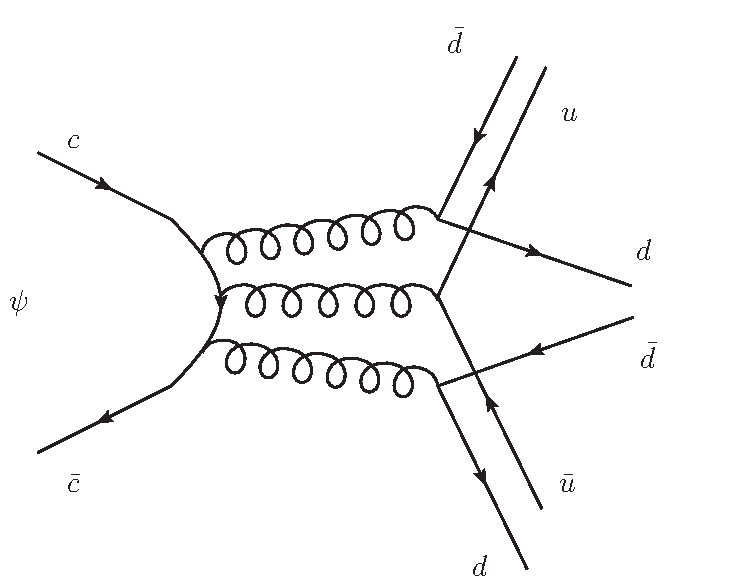
\includegraphics[width=0.6\textwidth]{Chapters/pQuarkonia/OZI.pdf}
 \caption{A \Jpsi decay to three gluons, suppressed by the OZI rule.}
 \label{fig:OZI}
\end{center}
\end{figure}
\\
What we have seen applies to $\phi$ mesons, as well as to % be leaving the $\phi$ on the side for now, and on
heavy quarkonium states, our main interest. The \Jpsi for instance, has a mass of $m_{\Jpsi} = 3.096~
\GeV/c^{2}$, which is smaller than the twice the $D^{0}$ mass. This
means that decays of the kind $\Jpsi \to D^{0}\bar{D}^{0}$ are
kinematically ruled out, leaving only QED annihilation and
OZI-forbidden hadronic decays. This results in an experimental width
of the order of 10 \keV, which was smaller than the experimental
resolution at that time! It is the combination of the $D$ meson observation above the
\Jpsi mass and the narrow width of $\psi$ states which definitely
identified the new resonances and hadrons as from a new quark flavour.
\\
\subsection{Production mechanisms: the hard part}
\label{sec:models}
One of the important questions of this Chapter (the question is likely to remain
unanswered), is whether we know what is (are) the production
mechanism(s) of quarkonia. 
I will restrict myself to the case of hadron-hadron collisions, but
there is also quarkonium production in electron-positron annihilation,
photoproduction, DIS. These channels have been very fertile and would require a whole separate
review, which I will not engage in.
\\
The hadron-hadron interaction can produce at tree level in QCD a pair of quark and
antiquark:
\begin{itemize}
% \item[-] a QED-mediated process, $q\bar{q} \to
% \gamma^{\star}/Z \to Q\bar{Q}$, which is usually called Drell-Yan,
\item[-] via QCD-annihilation $q\bar{q} \to Q\bar{Q}$,
\item[-] via gluon fusion and splitting, $gg \to Q\bar{Q}$.
\end{itemize}
 At the LHC, the large distribution of gluons inside each proton makes the gluon
 fusion the \textit{dominant} channel for large $Q^{2}$ and small-$x$ processes, which leads us to consider gluon
 fusion as the dominant initial state for quarkonium production in our
 review. Then comes the issue of the quantum
 numbers in the final state.
\\
We have J$^{PC}$ = 1$^{--}$ for \Jpsi and \PgU. From the OZI rule we
have seen that the decay of \Jpsi into one gluon is impossible
kinematically; Additionally, the two-gluon decay would
violate the charge conjugation parity, as the left part is C-odd, and
the right part is C-even.
\\
Strictly speaking, it is possible to turn the OZI rule around and
realise that the only way to produce a quarkonium with the correct
quantum numbers is by the
interaction of at least three gluons. A process with three gluons in the initial state
has a too small rate, that could not account for the measured
\Jpsi rate.

So at LHC energies, gluon fusion is dominant \textit{and} the
pre-quarkonium state formed has to emit gluons to equilibrate its
degrees of freedom of angular momentum and/or colour. This in some sense resembles
hadronisation, although we do not know what is the colour of the initial
state; Rather, nothing prevents the gluon fusion to produce a white or
a coloured $Q\bar{Q}$ pair at the partonic level a priori. It is only
afterwards when the pair hadronises that the colour is
equilibrated.


There are various ways to recover the proper quantum numbers for each
quarkonium wave function: in fact, when expanding to ever higher
orders of the perturbative $\alpha_{S}$ expansion, one finds an
infinity of terms contributing to quarkonium production. Some
models have been proposed to describe the production processes: 
\begin{itemize}
\item[-] The Colour Singlet Model (CSM)~\cite{CSM} assumes that quarkonia are directly
  produced with the `good' quantum numbers, i.e. the one they have
  when they decay: this poses strong
  constraints on either the kinematics or the total rate for producing
  a given state, as can be seen in Figure~\ref{fig:CDF_CSM};
\item[-] The Colour Octet Model (COM)~\cite{Braaten:1994vv} suggests that quarkonium production via
  a pre-resonant colour octet intermediate state would in fact matter,
  to the point where these extra terms may
  become dominant. In this point of view the CSM alone can not
  account for the spectrum of a given quarkonium and its integrated
  cross section at the same time;
\item[-] Non-Relativistic QCD (NRQCD)~\cite{nrqcd} tries to unify CSM and COM:
  Stating that a hard process can be factorised from the long distance
  hadronisation
  part, it details the amplitudes of quarkonium production as an
  expansion of terms involving a short distance (hard part) resembling
  the CSM, and a long distance matrix element (LDME) containing
  the color octet contributions. Given the fact that both quarks are heavy,
  they can be treated non-relativistically in the quarkonium rest
  frame;%, thus giving credit to the factorisation hypothesis;
\item[-] Finally, the Colour
  Evaporation Model (CEM)~\cite{Amundson:1996qr} suggests a quarkonium production following
  dynamics comparable to that of heavy flavour hadron pairs
  ($D\bar{D}$ in the case of charmonium, \textit{etc.}). % The model has
  % been given fame in the days of Tevatron and HERA days, when CSM was
  % strongly failing.
  In this case, the colour equilibration is treated
  as a nonperturbative process, related to the hadronisation phase.
\end{itemize}



% Before going into the details of each model, I would like to point out
% some group-theoretical aspect which helped in my personal
% understanding of the 'divide' between CSM and COM advocates.

% Making use of the fact that quarks form a triplet in the fundamental
% representation of QCD, one could construct the following equation:
% \begin{equation}
% \mathbf{3\times\bar{3} = 1 \oplus 8}
% \end{equation}
% Adding the quark degrees of freedom together to make a
% $Q\bar{Q}$ wavefunction, one can construct either a colour singlet or
% octet. All final state objects observed are colour singlets of course,
% so the existence of colour octet states or terms has to be temporary:
% the question whether this is a long scale or short scale process is
% relevant in this discussion, and that's where (I believe) the 'divide'
% stands between CSM and COM lies. That would seem trivial to
% experimentalists, but when making a detailed QCD calculation of the
% $Q\bar{Q}$ amplitude including leading and next-to-leading order terms
% for example, one may ask himself whether the colour octets can live
% outside the tree-level, parton world, or not.
% \\
% Authors Baier and Ruckl have argued in the past~\cite{CSM} that the quarkonium
% object could be produced dominantly as a colour singlet, the octet
% terms being suppressed with higher powers of $\alpha_{S}$. This led to what
% is known nowadays as the colour singlet model. In this framework, the $Q\bar{Q}$
% pair is produced in the correct quantum numbers at the partonic tree
% level, so a very small number of diagrams are needed to compute the
% amplitude. Only the binding between quarks remains non-perturbative. Unfortunately, the
% colour singlet model (CSM) has issues, some of which I want to detail here.
% \\
The \pt(\Jpsi) spectrum measured at CDF in $p\bar{p}$
collisions does not match the colour singlet (LO), neither
qualitatively nor quantitatively~\cite{CDFpsi}. At tree level (LO), the expected
\pt-spectrum behaves according to the CSM as $\pt^{-8}$, which disagrees strongly
with the experimental measurement of CDF, as one can see on both
panels of Figure~\ref{fig:CDF_CSM}.

\begin{figure}
\begin{center}
  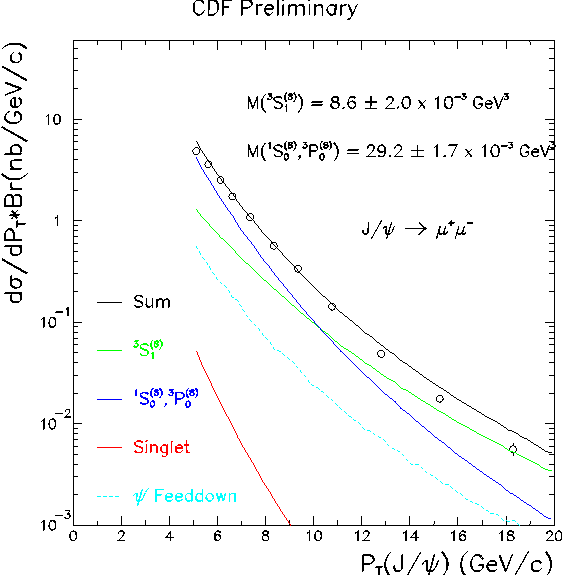
\includegraphics[width=0.45\textwidth]{Chapters/pQuarkonia/CDFpsi1S.pdf}
  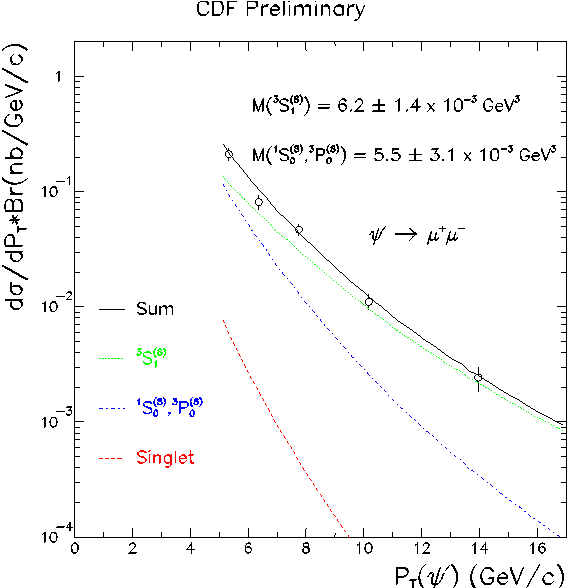
\includegraphics[width=0.45\textwidth]{Chapters/pQuarkonia/CDFpsi2S.pdf}
  \caption{Charmonium momentum distributions from
    CDF~\cite{CDFpsi}. Left, the \Jpsi spectrum compared to LO CSM and
    additional colour octet terms. Right: same computation for
    $\psi(2S)$.}
  \label{fig:CDF_CSM}
\end{center}
\end{figure}

 The left hand side specifically treats the
case of \Jpsi, and the $\psi(2S)$ case is presented on the right hand
side of
Figure~\ref{fig:CDF_CSM}. In the colour singlet hypothesis,
% poses strong constraints on the branching fractions from higher states
% (further referred to as feed-down fractions). Indeed, since
the quarkonium $\psi$ is produced from a gluon fusion process $gg \to ? \to \psi +
X$ with a colour singlet  wavefunction $\psi$ and its
allowed quantum numbers are that of $\eta$ ($^{1}S_{0}$) or
$chi_{0,2}$ ($^{3}P_{0,2}$). This would mean that all \Jpsi\ come from
radiative decays $\chi_{c} \to \Jpsi\gamma$, and all $\psi(2S)$ come
from $b$ decays. A measurement of the prompt $\psi(2S)$ rate compared
to the non-prompt $b \to \psi(2S)$ rate, by the CDF collaboration in 1994, has shown
that the theoretical prediciton were in an order of magnitude of
disagreement with the experimental data~\cite{CDF:1994aa}.

% This did not 'kill' the CSM
% instantly, as one starts to imagine that refined NLO QCD corrections come into
% play. We shall see that CSM predictions to higher orders are still
% used today by experiments to compare with their quarkonium
% data. Still, one can argue that a higher order term can only be
% smaller than the previous order, otherwise the perturbative limit is
% not satisfied and the whole expansion is meaningless. However, the
% criticism arguing whether the CSM really has a sound theoretical basis
% is out of the scope of this here discussion.







\subsection{Quarkonium spectroscopy}
\label{sec:spectro}
Associating a quark and an antiquark of the same flavour (often called
hidden heavy flavour) in a bound state will
result in a constrained spectroscopy. One can find common examples of
simple semi-classical systems (treated quantum mechanically, but where
the dynamics are non-relativistic) such as the positronium system or
the hydrogen atom, or the H$_{2}$ molecule, that would produce
comparable classifications of energy levels. Of course the quantum formalism
would be that of QED, and since we are interested in QCD in this case, the analogy
has some limitations. Nonetheless, one can model an effective
quarkonium potential of the form that was used in
Equation~\ref{eq:potential} and solve the Schrödinger equation, to
extract a spectroscopy, i.e. energy levels that can be compared to
experimental data by simply measuring the mass of each resonance
discovered. 
\\
\begin{figure}
\begin{center}
  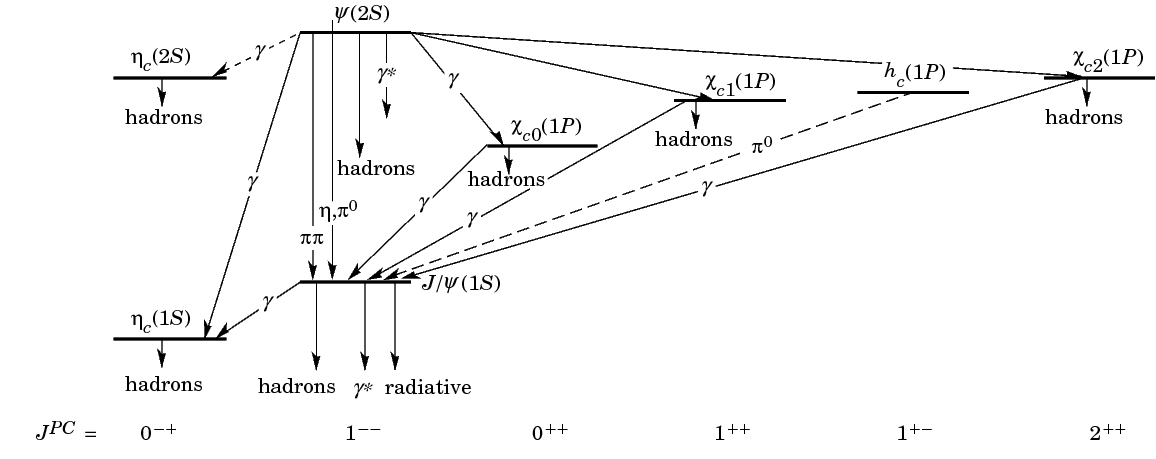
\includegraphics[width=0.9\textwidth]{Chapters/pQuarkonia/charmonia.png}
  \caption{Charmonium spectroscopy. The abscissae are J$^{PC}$ indices
  (spin, parity, charge conjugation). From~\cite{spectro}.}
  \label{fig:charmonium}
\end{center}
\end{figure}
\\
For both charm and beauty, the spectroscopy begins with a ground state
with quantum numbers $n=0$, $L=0$, $S=0$, $J=0$, which is usually
identified as an $\eta_{c}$ or an $\eta_{b}$ meson. One finds higher energy bound states of various quantum numbers up
to the $D^{0}\bar{D}^{0}$ 
threshold or the $B^{0}\bar{B}^{0}$ threshold, for charm and beauty
respectively. Above the threshold, the inital $Q\bar{Q}$
system contains enough rest energy to decay dominantly in $D$ or
$B$ mesons. Resonances existing above this threshold are far wider, as for
example $\Upsilon(4S), \Upsilon(5S), \Upsilon(6S)$. For these, all
OZI-favored hadronic transitions are measurable, hence their very
large width (for example $\Gamma(\Upsilon(4S)) / \Gamma(\Upsilon(nS))
\approx 500$ for n < 4).

The charmonium spectroscopy is depicted in Figure~\ref{fig:charmonium}. All
states appearing are below the $D\bar{D}$ threshold. Other states have
been discovered, for which a very consequent review is done by the
Quarkonium Working Group~\cite{nora}. The simplest possible
transitions are drawn with arrows, and correspond to radiative
deexcitations (dipolar electric E1 transitions) or emission of one or
several light hadrons.


\begin{figure}[htb]
\begin{center}
  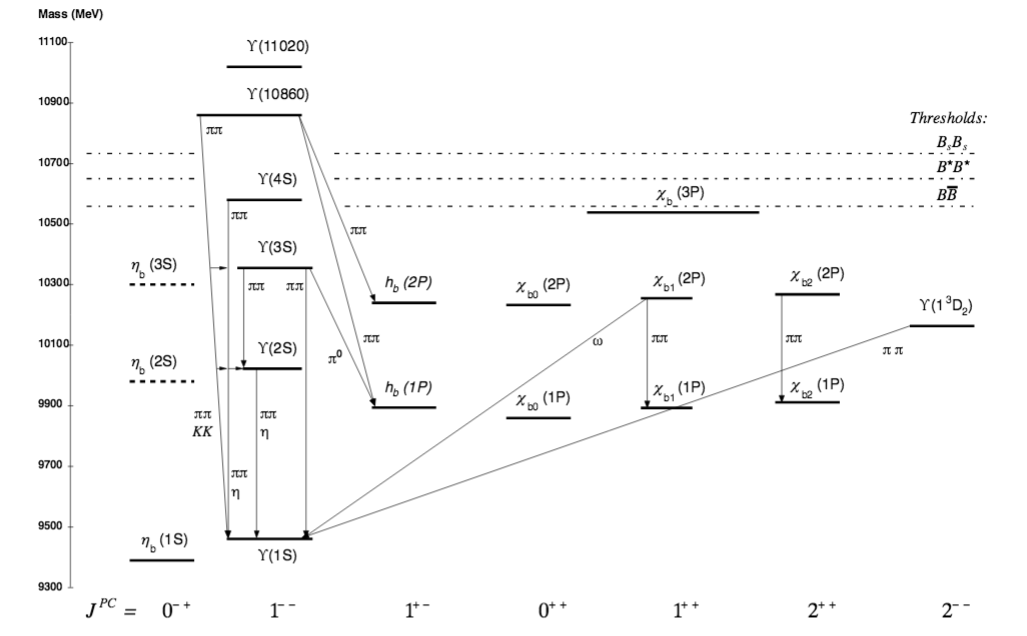
\includegraphics[width=0.7\textwidth]{Chapters/pQuarkonia/bottomonium.png}
  \caption{Bottomonium spectroscopy. The abscissae are J$^{PC}$ indices
  (spin, parity, charge conjugation). The vertical axis, not
  displayed, would represent increasing theoretical rest masses. From~\cite{spectro}.}
  \label{fig:bottomonium}
\end{center}
\end{figure}
\vspace{0.3cm}
For bottomonia, the picture is somewhat more complicated by the larger
gap between the ground state mass and the $B\bar{B}$ threshold. As one
can see on Figure~\ref{fig:bottomonium}, the spectroscopy resembles
that of charmonium, as expected. The recently discovered $\chi_b(3P)$
state~\cite{chib3p,chib3p_lhcb} does not appear in this picture and
would stand between $\chi_b(2P)$ and the $B\bar{B}$ threshold.
\\
The transitions from excited states to lower levels of the bottomonium
family, called feed-down
fractions, are summed up in Figure~\ref{fig:hermine}. These
fractions represent the ratio of cross sections for bottomonium states
decaying into another, as a function of the product \PgU~\pt. Here are of
interest the radiative E1 transitions $\chi(mP) \to \PgU(nS)$, with $n\leq
m-1$ and the hadronic transitions $\PgU(nS) \to \PgU(n'S)$, with $n'
\leq n-1$. As we can anticipate, the kinematics of the decay constrain the
total \PgU~decay
rate, and this has in the past led to misconceptions regarding
feed-down fractions of \PgUa~from higher states. These feed-down
fractions may be crucial to interpret the suppression 
pattern of quarkonium modification or suppression in heavy ion collisions.


\begin{figure}[htb]
\begin{center}
  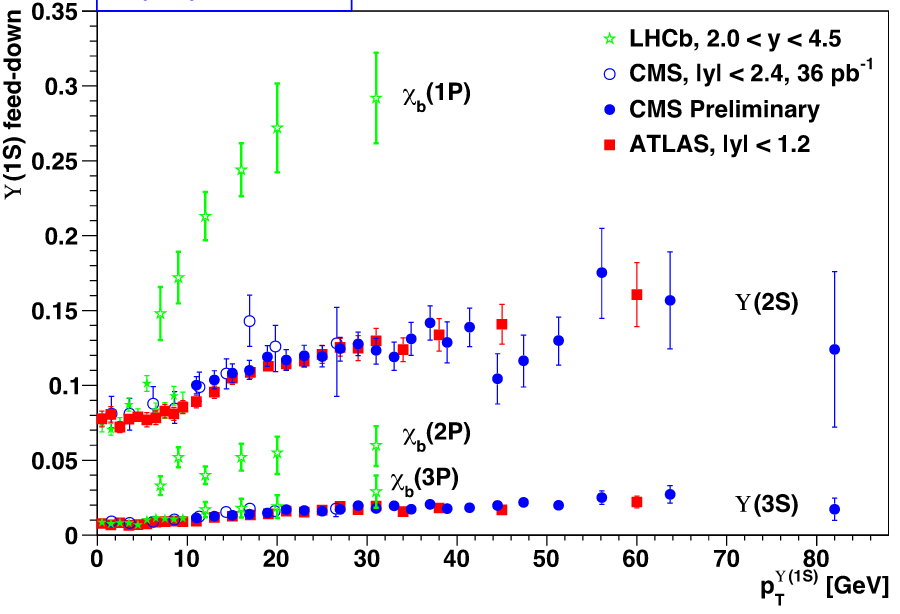
\includegraphics[width=0.8\textwidth]{Chapters/pQuarkonia/feeddown.png}
  \caption{Feed-down fractions of excited bottomonia to \PgUa, as a
    function of the transverse momentum of the \PgUa\ meson. From~\cite{hermine}}
  \label{fig:hermine}
\end{center}
\end{figure}


\vspace{0.5em}
\begin{center}
  \fbox{
    \parbox{0.9\textwidth}
    {\textsf {In this section the basis of our understanding of
        quarkonium production in vacuum was presented. The
        experimental data from Tevatron provided a long standing
        puzzle to a theoretical formulation that would reproduce the
        data. However, with newer high-luminosity experiments such as
        the LHC or future experiments, a larger understanding of
        quarkonium production in $pp$ can be possible.}}} 
\end{center}



\section{Charmonia in nuclear matter}
% In vacuum, the charmonium states are very well measured. There are
% many reviews of the charmonium physics. Experimentally, one of the
% causes of resurgence in charmonium physics was the impossibility
% to match the \Jpsi spectrum from Tevatron data to leading order (LO)
% and next-to-leading order (NLO) calculations.

% Nowadays the frameowrk of NRQCD works quite well at reproducing parts
% of the spectrum of charmonium states. The LHC has produced impressive
% results for the \pt spectrum of \Jpsi, $psi'$ and $\chi_{c}$ states,
% as well as measurements of exotic states as $X(3872)$.
\subsection{At the SPS}

% Starting with NA3 collaboration data, the $x_{F}$ dependence of \Jpsi
% production is measured with good precision. Later measurements at HERA
% in $ep$ and $eA$ collisions presented interesting constraints to the gluon PDF:
% there, quarkonium photoproduction is highly-driven by the kinematics
% of the gluon in the nucleon or the nucleus, and the comparison of both
% gives a good constraint on $xg$.

The
CERN SPS fixed target experiments NA38, NA50 and NA60 investigated the
charmonium sector in various heavy ion systems ($pp$, $p$-A, A-B, A-A,
with various ions A and B), to look for the onset of suppression~\cite{Baglin:1990iv,Abreu:1997jh,Abreu:2000xe,Abreu:2000ni,Alessandro:2004ap,jpsiNA60}. In all cases, the
experiment could use multiple targets, allowing for a precise scan of
the energy density dependence of the collision. 

Each experiment reconstructed dimuon invariant mass pairs in the
charmonium region and around, to measure the signal and background
constributions. The \Jpsi and $\psi(2S)$ cross sections were extracted
from other same-charge background dimuon sources % such as open charm, Drell-Yan and
% combinatorics from $\pi$ and $K$ decays~\cite{Alessandro:2004ap}.
In order to measure the centrality,
one could record the energy deposited in zero degree calorimeters
(ZDC) or using the multiplicity in a nearby silicon tracking device, and
later use a Glauber model calculation to extract an effective length $L$ of
nuclear material seen by the probe. The Drell-Yan cross section
$\sigma(A+B \to \mu^+\mu^-)$, measured
around the \Jpsi peak (2.9 < $m_{\mu\mu}$ < 4.5~\unitMass)~\cite{Alessandro:2004ap}, is used as a
reference in all collision setups to compare with the~\Jpsi cross
section, as is shown on Figure~\ref{fig:na60}.



\begin{figure}[htb]
\begin{center}
  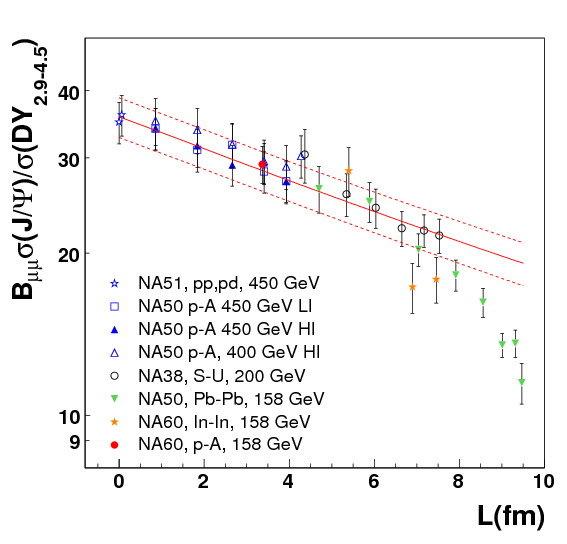
\includegraphics[width=0.6\textwidth]{Chapters/pQuarkonia/NA60.png}
  \caption{\Jpsi suppression from SPS experiments as a function of
    nuclear length $L$. From~\cite{compilSPS}.}
  \label{fig:na60}
\end{center}
\end{figure}



The green points represent what was called an 'anomalous'
suppression, in the sense that above $L = 7$ fm the observed data does not
conform to pure nuclear absorption. The  nuclear absorption is
estimated using a Woods-Saxon nuclear distribution fitted to data,
exhibiting an absorption cross section of $\sigma_{\rm {abs}}= 4.18 \pm
0.35$ mb.%  This suppression can be further investigated by separating
% charmonium states \Jpsi and $\psi(2S)$. Figure~\ref{fig:psi2SPS}




% In itself, Figure~\ref{fig:na60} is not a definite proof of melting in
% heavy ions collisions. First, the observed suppression for \Jpsi
% contains feed-down from $\psi(2S)$ and $\chi_{c}$, for which the plot
% does not tell the suppression pattern. Second, the nuclear length $L$
% compares different collision geometries in pA, AA (A = Pb, In, \textit{etc.})
% and hence might be inadequate. A further measurement of more than just
% \Jpsi, extending at higher number of participants or at higher
% energies is needed to disentangle nuclear absorption from
% QGP. 
\subsection{At RHIC}

Studies to find the effects of deconfinement progressed at Brookhaven
with the start of RHIC (Relativisitc Heavy Ion Collider) operation
in 2000.
The charmonium system was measured there in pp collisions at \s\ = 500
GeV, in deuteron-gold (dAu) and gold-gold (AuAu) collisions at \snn\ =
200 GeV.

The dependence of charmonium suppression was investigated there as a
function of transverse momentum, rapidity and centrality percentiles,
the latter instead of nuclear matter length. The centrality is again obtained via a
Glauber model calculation, which in the case of the PHENIX experiment,
is correlated to the collected charge in the Beam Beam
Counters (BBC). A complete review of centrality measurements for AuAu
and dAu collisions with the PHENIX detector from RHIC is available
in~\cite{centralityRHIC}.
\begin{figure}
\begin{center}
  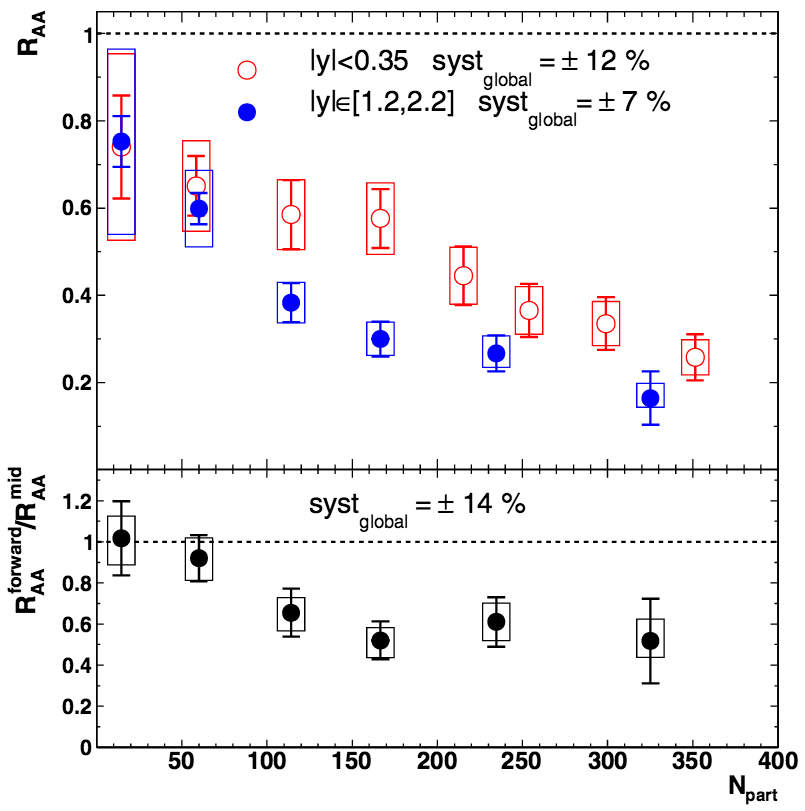
\includegraphics[width=0.5\textwidth]{Chapters/pQuarkonia/Phenix_raa_centrality.png}
  \caption{\Jpsi suppression in AuAu collisions at \snn~=~200 GeV from PHENIX at RHIC, as a function of
    centrality. Two rapidity regions are shown: central (open symbols),
    forward (closed symbols). From~\cite{jpsiphenix}.}
  \label{fig:phenixnpart}
\end{center}
\end{figure}
Figure~\ref{fig:phenixnpart} shows the centrality dependence of \Jpsi
suppression at \snn\ = 200 GeV from PHENIX. The \Jpsi yields are
measured in the central region (open symbols) and in the forward
direction (blue). This seems to show that the \Jpsi is more suppressed
at RHIC in the forward direction, which is counterintuitive: indeed
the energy density is expected to be higher in the central rapidity
region, which would lead to more suppression in the central arm.

% As to compare with the anomalous suppression of SPS, the situation now
% worsens with this new anomaly. In contrast, 
The \Jpsi suppression from fixed target experiments at SPS energies was
probing regions of the Bjorken-$x \approx 0.1$, a region where the gluon density is
relatively unmodified in nuclei, compared to the $x$ regime of PHENIX
measurements (smaller $x$ values, typically $10^{-3} < x <
10^{-2}$). In this small-$x$ region, the gluon density can suffer a depletion
(\textit{shadowing}) effect in nuclei, resulting in a \Jpsi yield
slightly affected downwards. The nuclear modification factor in dAu
from PHENIX~\cite{jpsiphenixdAu}, $R_{dAu}$ is presented in
Figure~\ref{fig:dAuphenix} (left) and
presents indeed some suppression in the p-going direction, which is in
this case positive rapidities.




\begin{figure}[th]
\begin{center}
  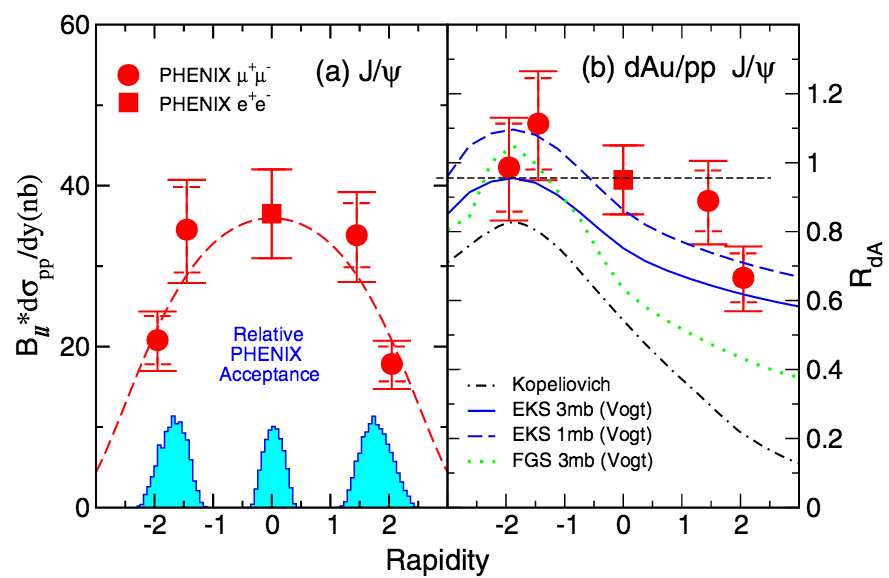
\includegraphics[width=0.5\textwidth]{Chapters/pQuarkonia/Phenix_rday.png}
  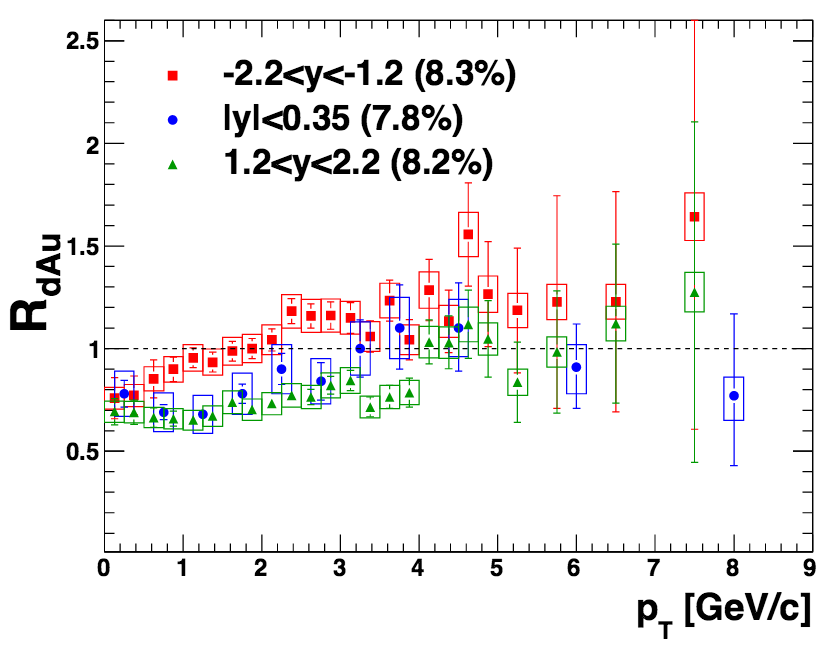
\includegraphics[width=0.42\textwidth]{Chapters/pQuarkonia/Phenix_rdapt.png}
  \caption{\Jpsi suppression in dAu collisions at \snn~=~200 GeV
    measured by the PHENIX experiment at RHIC, as a function of
    \Jpsi rapidity (left) and transverse momentum (right). From~\cite{jpsiphenixdAuy,jpsiphenixdAupt}.}
  \label{fig:dAuphenix}
\end{center}
\end{figure}



One can also notice on Figure~\ref{fig:dAuphenix} (right) the \pt
dependence of the \Jpsi dAu suppression. The \Jpsi seems to be
slightly suppressed in low transverse momenta. This \pt-dependent
measurement of the suppression in dAu need to be completed with a
measurement involving two ions, to see if any additional suppression
is thus also reflected in the AA \pt\ spectrum.


\begin{figure}[th]
\begin{center}
  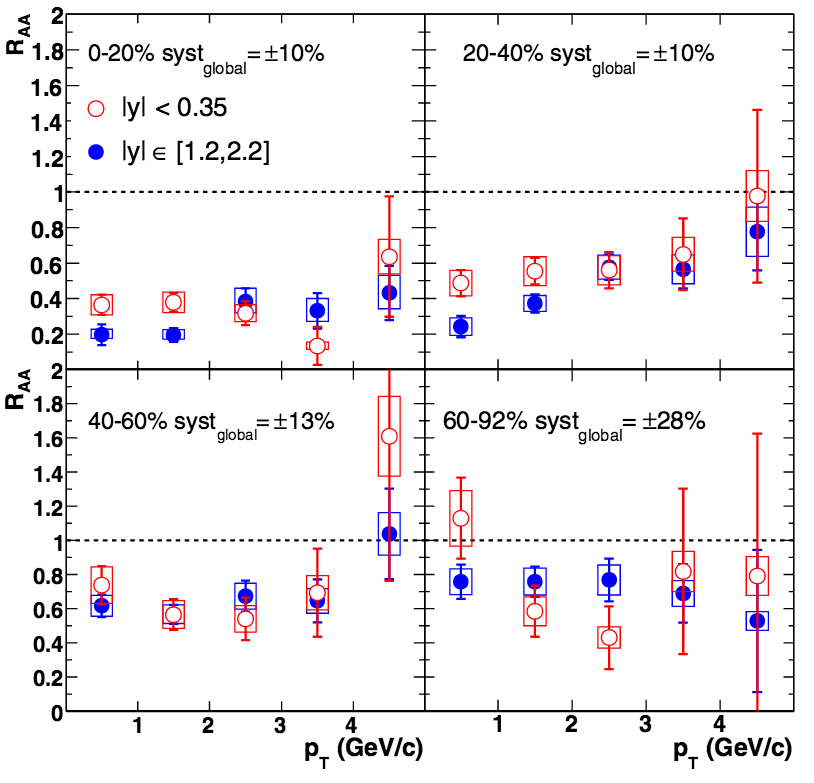
\includegraphics[width=0.8\textwidth]{Chapters/pQuarkonia/Phenix_raa_pt.png}
  \caption{\Jpsi suppression in AuAu collisions at \snn~=~200 GeV
    measured with the PHENIX experiment at RHIC, as a function of
    \Jpsi transverse momentum. The four panels from top left to bottom
    right correspond to decreasing centrality classes. Open symbols:
    central rapidity, closed symbols: forward rapidity. From~\cite{jpsiphenix}.}
  \label{fig:AuAuphenixpt}
\end{center}
\end{figure}


Thanks to RHIC data, the suppreesion of \Jpsi in AuAu and $d$Au has been
clearly measured, to finally reach a lowest suppression point of
approximately \RAA $\approx$ 0.2 in
 low-\pt central AuAu collisions. In Figure~\ref{fig:AuAuphenixpt} the
 \pt-dependence of \Jpsi in AuAu collisions is presented with various
 centrality classes. The suppression seems to be stronger in high centrality,
 low-\pt events. However, a mild difference between forward and
 central rapidities is observed, and could be explained by more
 nuclear absorption setting in at forward rapidities, or a
 possible gluon shadowing effect. 

\clearpage
\subsection{At the LHC}


At the LHC, the energy in the centre-of-mass for PbPb collisions is \snn~=
2.76 TeV for the first operation period (Run1, up to 2013). The center
of mass energy in pPb is \snn~= 5.02 TeV, while pp data was taken at
\s~= 2.76, 7, 8 TeV.
The ALICE and CMS experiments have measured \Jpsi~yields with high
precision in pp, pPb and PbPb, yielding several suprises. First of
all, the suppression measured at ALICE is much less pronounced at low
transverse momentum than in the RHIC data, as is shown on
Figure~\ref{fig:aliceJpsi} (left). This plot also has \Jpsi data from
the CMS collaboration (prompt \Jpsi, \pt > 6.5 \GeVc) in the central
rapidity region. The right hand side of Figure~\ref{fig:aliceJpsi} has the
rapidity dependence of inclusive \Jpsi suppression in PbPb, exhibiting
less suppression at midrapidity than at RHIC
(cf. Figure~\ref{fig:AuAuphenixpt}), and a stronger suppression when
going to higher rapidity ranges.

\begin{figure}[h]
\begin{center}
  \includegraphics[width=0.48\textwidth]{Chapters/pQuarkonia/Aliceraapsipt.png}
  \includegraphics[width=0.48\textwidth]{Chapters/pQuarkonia/Alicepsipbpby.png}
  \caption{\Jpsi suppression in PbPb collisions at LHC energies, as a function of
    the \Jpsi \pt in ALICE forward data and CMS data (left), and as a
    function of \Jpsi rapidity with ALICE (right). Red squares:
    forward rapidity, blue circles: central rapidity. Black squares:
    CMS high \pt data. From~\cite{jpsiALICE}.}
  \label{fig:aliceJpsi}
\end{center}
\end{figure}



On Figure~\ref{fig:alicenpart}, the
centrality dependence is presented, and appears saturating at $\RAA \sim$ 0.65 from \Npart\ = 100. When comparing with RHIC results,
this looks like a strong enhancement, or a much weaker
suppression. Models accounting for statistical recombination of
decorrelated charm quarks~\cite{BraunMunzinger:2000px,Grandchamp:2002wp} into \Jpsi\ suggest that at LHC energies, the
energy density is such that about 100 $c\bar{c}$ pairs are produced in
central PbPb events, leading to a large probability for these quarks
to combine in the hadronic freeze out phase in a \Jpsi\ (or $\psi(2S)$)
state, hence populating the spectrum and reducing the observed
suppression in this phase space region.
\begin{figure}[h]
\begin{center}
  \includegraphics[width=0.65\textwidth]{Chapters/pQuarkonia/Aliceraanpartpsi.png}
  \caption{\Jpsi suppression in PbPb collisions from ALICE, as a function of
    the centrality of the collision. Red squares:
    forward rapidity, blue circles: central rapidity. From~\cite{jpsiALICE}.}
  \label{fig:alicenpart}
\end{center}
\end{figure}



The CMS collaboration has published a \pt, rapidity and centrality dependent \Jpsi
result~\cite{torsten} for high \pt \Jpsi (prompt and non-prompt,
i.e. coming from secondary displaced vertices). The \RAA was further
 recently updated with higher statistics in pp data in~\cite{12014} and is
presented in Figure~\ref{fig:CMSpsi}.
\begin{figure}[h]
\begin{center}
  \includegraphics[width=0.7\textwidth]{Chapters/pQuarkonia/CMSPromptJpsi.pdf}
  \includegraphics[width=0.7\textwidth]{Chapters/pQuarkonia/CMSNonPromptJpsi.pdf}
  \caption{high \pt \Jpsi suppression in PbPb collisions from CMS, as a function of
    the centrality of the collision. Top: prompt \Jpsi, Bottom:
    non-prompt \Jpsi. From~\cite{12014}.}
  \label{fig:CMSpsi}
\end{center}
\end{figure}



There may be nuclear
modification process(es) affecting the \Jpsi~production (pPb data from CMS~\cite{14009} and
ALICE~\cite{alicejpsipPb} that I have not covered here, and that seem to go in the direction
of a reduction of the \Jpsi~yield in cold nuclear matter). Finally, there is a lot of interest regarding the $\psi(2S)$
suppression in PbPb collisions. First, this is a very challenging measurement
given the naturally small $\psi(2S)$ yield when comparing with
\Jpsi. Second, a measurement from CMS~\cite{Khachatryan:2014bva} seems to show less suppression
for $\psi(2S)$ than for \Jpsi\ in an intermediate \pt\ region, where
some recombination effects could still be at play. This would only be
settled with a careful look at a more abundant PbPb dataset in the
coming years. In 2015, the LHC will operate Pb ion beams reaching an energy
in the center of mass of about 5 TeV, which will allow one to reach even
higher energy densities than previously, and will enhance slightly the
cross section for hard processes such as the \Jpsi\ and $\psi(2S)$.



% \vspace{0.5em}
% \begin{center}
%   \fbox{
%     \parbox{0.9\textwidth}
%     {\textsf { }}} 
% \end{center}

\clearpage
\section{The bottomonium case}

Since the $b$ quark mass is higher than the $c$ quark, it is likely that
perturbative calculations find a better agreement on \PgU~data than
what was observed in \Jpsi data. Also, one can make a more stringent test of the
non-relativistic hypothesis given the higher quark mass.
Although the feed-down fractions were known from \pt = 8 \GeVc and
above with Tevatron data, the LHC measurements provide with more
information on the transition from higher energy levels to the ground
state, which is an important constraint for our understanding of
\PgU~suppression in heavy ion collisions. The feed-down fractions from
\PgU(nS), $\chi_{b}$(mP), to \PgUa~were previously shown on
Figure~\ref{fig:bottomonium}.
\\
Next I will move to the case of bottomonia in heavy ions. The melting
temperature is expected to be different for states with different
binding, hence it is interesting to look for the yields of all three \PgU~states in
heavy ion collisions. These provide interesting constraints on the temperature of
the medium produced in heavy ion collisions at the energies of the LHC (as well
as RHIC energies as we shall see). In the case of \PgU~states, the
mass being larger than for charmonia, it is possible that binding
energies from potential models are more stable. When it comes to the nuclear
absorption effects and shadowing, these should also be smaller than
for charmonia, given the fact that the initial parton is slightly
harder. Finally I will present some results regarding \PgU\
measurements as a function of the event centrality in PbPb collisions
that exhibited a strong suppression of the excited states for the
first time, shortly before the beginning of my thesis.

\subsection{\texorpdfstring{\PgU}{Y} production in pp collisions}
The LHC data collected during Run 1 provides several useful
constraints on quarkonium production, and that is seen for \Jpsi
as well as for \PgU. We now turn to the case of \PgU~production in pp collisions.



The ATLAS experiment measures \PgU~states decaying in two muons in the
pseudorapidity range $\vert\eta^{\mu}\vert < 2.25$. %  (the branching
% fraction for \PgUa~to
% muons is $B_{\mu\mu} = 2.78 \%$).
This measurement in 7 TeV pp data~\cite{atlasUpsilon7tev} 
scans the \pt spectrum up to 70 \GeVc~with an integrated luminosity of $\lumi$ = 1.8 \invfb. The invariant mass plot for the central rapidities
$\vert y\vert <
1.2$ appears in Figure~\ref{fig:upsimass_pp} (top, left). 



CMS has measured \PgU~states in the dimuon channel with pp data at 7
TeV as well, dedicating two papers (post-ICHEP
2010 which consisted of about 3~\invpb~of 2010 data). The first
publication~\cite{cmsUpsi1} presented \PgU~spectra up to \pt = 50 \GeVc, with
approximately 36~\invpb~of pp data, using the full coverage of muon
detectors and of the inner tracking system, $\vert\eta\vert <
2.4$. Next, a further measurement~\cite{cmsUpsi2} using $\lumi$ = 4.9
\invfb of pp data focuses on events with $\pt > 10~\GeVc$ with a rapidity
cut at $\vert y^{\mu\mu}\vert < 1.2$, where the dimuon resolution is as good as
to separate clearly the three upsilon states, as shown in
Figure~\ref{fig:upsimass_pp} (top, right).

\begin{figure}[h]
\begin{center}
 \hspace{0.5cm} \includegraphics[height=0.2\textheight]{Chapters/pQuarkonia/AtlasUpsi.pdf}
  \includegraphics[height=0.21\textheight]{Chapters/pQuarkonia/CMSUpsi.pdf}
  \includegraphics[height=0.21\textheight]{Chapters/pQuarkonia/lhcbUpsi.pdf}
  \includegraphics[height=0.21\textheight]{Chapters/pQuarkonia/AliceUpsi.png}
  \caption{The dimuon invariant mass distribution in the vicinity of
    the \PgU\ resonances for ATLAS data (top, left), CMS data (top,
    right), LHCb data (bottom left) and ALICE data (bottom right). The
    solid lines in ATLAS, LHCb and ALICE plots represent fits to the invariant mass distributions, as
  described in respective publications~\cite{atlasUpsilon7tev,lhcbUpsi1,aliceUpsi_pp}.}
  \label{fig:upsimass_pp}
\end{center}
\end{figure}


The LHCb collaboration has also measured \PgU~states in $\lumi = 36~\invpb$
of pp collisions at \s\ = 7 TeV, in a publication extending to events with $\pt < 15
\GeVc$, in the dimuon rapidity coverage of LHCb ($2.5 < y <
4$)~\cite{lhcbUpsi1}. The dimuon invariant mass plot in the \PgU~mass
range is presented in Figure~\ref{fig:upsimass_pp} (bottom, left).
%  A more recent LHCb paper~\cite{lhcbUpsi1fb} using
% \s\ = 7 TeV and \s\ = 8 TeV data has also been published, from which the
% \pt\ spectrum is displayed in Figure~\ref{fig:upsispectrapp}
% (bottom, left).


% but since the data set is not
% particularly larger than in~\cite{lhcbUpsi1} 7 TeV data, the
% comparison I am doing here relies on 7 TeV data only. Nevertheless one
% does not expect a lot of change between 7 TeV and 8 TeV quarkonium
% data, except a slightly higher cross section (as for other hard
% processes, the $Q\bar{Q}$ cross section increases with \s).



The ALICE collaboration has measured quarkonium states in 7 TeV
collisions as well, with $\lumi = 1.35 \invpb$ of pp data, recorded in the
rapidity range $2.5 < y < 4$. The measurement~\cite{aliceUpsi_pp} extends to \pt = 12
\GeVc, and the invariant mass plot is presented in
Figure~\ref{fig:upsimass_pp} (bottom, right).



The various mass plots of Figure~\ref{fig:upsimass_pp} are all
different in that they do not all span the same phase space window,
and the detector settings vary from one experiment to the other. The
unexhaustive details given here are based on the four plots of
Figure~\ref{fig:upsimass_pp}:
\begin{itemize}
\item[1.]{CMS and ATLAS invariant mass figures (upper panels of
    Figure~\ref{fig:upsimass_pp}) cover the mid-rapidity region,
    $\vert y \vert < 1.2$. The analyses performed in the two experiments are
    comparable, in terms of reconstruction and trigger strategies. As
    a consequence, the only difference comes from the mass resolution
    of the peaks: in ATLAS, the reported $\Upsilon(1S)$ width is 120
    MeV, while in CMS it is roughly two times less (the actual number
    for the presented plot was not made public). The broader peak seen
    in ATLAS is explained by the smaller magnetic field intensity,
    rendering a poorer momentum resolution on individual muons. The
    momentum resolution in both experiments is of the order of 1 to 5
    \% for \Jpsi\ muons, as reported in~\cite{Aad:2014rra,CMS:2010oua}.}
\item[2.]{ALICE and LHCb have similar rapidity coverage, $2.5 < y <
    4$, a region where the dimuon mass spectrum can
    be populated with combinatorial background exponentially
    decreasing with increasing dimuon mass, as is seen in both figures
    (lower panels of
    Figure~\ref{fig:upsimass_pp}).}
\end{itemize}


The \pt spectra are measured in all four experiments, and presented
in Figure~\ref{fig:upsispectrapp}. The differential cross sections are
computed after extracting the yield from invariant mass plots similar to what is
shown on Figure~\ref{fig:upsimass_pp}, with a differential binning in
the observable under consideration, \pt\ or \y. The extraction is performed using
empirical functions to describe the signal and background, which are
fitted to data. For each peak, as is shown in
Figure~\ref{fig:upsimass_pp} (top, left and bottom, right) there is a
different fit curve, and each curve is integrated to get a raw
yield for the considered \PgU~state. The yield is further corrected
for effects relative to the detectors inefficiencies or inadequate
modeling. Applying the proper luminosity normalisations and efficiency
corrections, one can derive a differential cross section times
branching fraction for the signal observed in the dimuon channel (as
it would be the case in our analysis).
\\
\begin{figure}[h]
\begin{center}
 \hspace{0.5cm} \includegraphics[height=0.25\textheight]{Chapters/pQuarkonia/AtlasUpsiPtNude.pdf}
  \includegraphics[height=0.25\textheight]{Chapters/pQuarkonia/CMSUpsiPt.pdf}
  \includegraphics[height=0.25\textheight]{Chapters/pQuarkonia/lhcbUpsiPtTsallis.pdf}
  \includegraphics[height=0.23\textheight]{Chapters/pQuarkonia/AliceUpsiPtCSCONLO.png}
  \caption{Transverse momentum dependence of \PgU~states' production
    in pp data at 7 TeV. Data from ATLAS (top, left)~\cite{atlasUpsilon7tev}, CMS (top,
    right)~\cite{cmsUpsi1},~\cite{cmsUpsi2}, LHCb (bottom left)~\cite{lhcbUpsi1fb}, and ALICE (bottom right)~\cite{aliceUpsi_pp}. The
    CMS data displayed also contains low-\pt results from a 2010
    analysis~\cite{cmsUpsi1}, scaled to account for the
    rapidity range difference with~\cite{cmsUpsi2}. The LHCb data is
    fitted with a Tsallis distribution function as described
    in~\cite{lhcbUpsi1fb}. The ALICE data is compared to a NLO
    prediction of quarkonium production in the NRQCD approach~\cite{nrqcdupsilon}.}
  \label{fig:upsispectrapp}
\end{center}
\end{figure}



After having applied all corrections that give a proper image of the
physical rate of \PgU~production in the experiment, one can compare to
theoretical models, such as the ones presented in Section~\ref{sec:models}.
With their larger mass, the perturbative calculations in QCD are
expected to yield more accurate results on bottomonia than what we have seen previously
for \Jpsi. 

Figure~\ref{fig:atlasNNLO} shows a theory comparison of ATLAS \PgUa~cross section results to the CSM
expectation, scaled to a normalisation factor, and the
CSM calculation is taken up to some terms of the
$\mathcal{O}(\alpha_{S}^{5})$ expansion, that is,
at partial next-to-next-to-leading order
(NNLO$^{\star}$)~\cite{LansbergNNLO}. The star symbol is 
here to indicate that the only NNLO terms considered in this
calculation are those considered by the author of~\cite{LansbergNNLO}
to give a dominant contribution in the $\alpha_{S}^{5}$. As is shown
in the first
bottom panel of the figure, the NNLO$^{\star}$ prediction drops faster
than the data at high \pt. Another
comparison visible in the lowest panel of Figure~\ref{fig:atlasNNLO}
is the CEM expectation, and this one shows another disagreement, again
with large uncertainties. The blue band associated with data points
results from a variation of polarisation hypotheses. Spin
alignment measurements have been since performed, for example with CMS
$\Upsilon$ data, for which the result will be presented below.
\\
\begin{figure}
\begin{center}
  \includegraphics[height=0.4\textheight]{Chapters/pQuarkonia/AtlasUpsiPt.pdf}
  \caption{\PgUa~differential cross section as a function of \pt, from
    ATLAS 7 TeV pp data~\cite{atlasUpsilon7tev}. Model comparisons
    include a truncated $\mathcal{O}(\alpha_{S}^{5})$ calculation
    (NNLO$^{\star}$) from the colour singlet model (CSM), in an orange
    uncertainty band, compared to data in the intermediate panel. The
    bottom panel has a colour evaporation model (CEM) prediction compared to
    data. On all panels, the blue band corresponds to a variation of
    the acceptance corrections with maximal longitudinal and transverse polarisations.}
  \label{fig:atlasNNLO}
\end{center}
\end{figure}



The ALICE \PgUa~\pt~spectrum in Figure~\ref{fig:upsispectrapp} shows a
comparison with NRQCD (that is, including colour singlet and
colour octet contributions) at NLO, which seems to find quantitative agreement
at high \pt. As mentioned in Section~\ref{sec:models}, one should note that NRQCD developments~% (which
% are usually done over the whole phase space, contrary to what is
% displayed here) 
predict a large transverse polarisation for \Jpsi or \PgU\ resonances, saturating
to an almost full transverse polarisation at high \pt. One should then
compare NRQCD expectations to the polarisation of measured quarkonia
in hadron-hadron collisions to look for a possible agreement.



CMS has published a measurement of the polarisation of all three
\PgU(1S,2S,3S) states in pp collisions in~\cite{CMSupsipol}. The
results for \PgUa\ and \PgUc\ are displayed in Figure~\ref{fig:upsipol}. It shows a helicity component $\lambda_{\vartheta}$ compatible with
zero for both \PgUa\ and \PgUc, and is overlayed with a theory
comparison in the case of~\PgUc. As one can see, in the NRQCD
formalism and contrary to the CSM, colour octet and higher order
contributions should exhibit a transverse polarisation for S-wave
quarkonia. Unfortunately, the agreement seen in \pt spectra
(relatively good, given uncertainty bands) should be taken with
caution because of this.
\begin{figure}[h]
\begin{center}
  \includegraphics[height=0.25\textheight]{Chapters/pQuarkonia/cmscdfupsipol1.pdf}
  \includegraphics[height=0.25\textheight]{Chapters/pQuarkonia/CMSCDFupsipol3.pdf}
  \caption{\PgUa~and \PgUc~polarisations measured by CMS in $pp$ and
    compared to CDF (Tevatron) in $p\bar{p}$ collisions as a function
    of \pt. The vertical axis corresponds to 
    the polarisation component in the helicity frame (HX). Taken from~\cite{CMSupsipol}.}
  \label{fig:upsipol}
\end{center}
\end{figure}
To elaborate more on comparisons with NRQCD without going into polarisation details
(which may be poorly constrained when the prediction is restricted to a
phase space region), I would like to end with a comparison of LHCb
cross section data from~\cite{lhcbUpsi1fb} for \PgU(1S,2S,3S) versus
\pt and rapidity. Figure~\ref{fig:crosssectionratiolhcb} shows the
ratio of such cross sections at the two \s\ = 7 and 8
TeV energies, $\mathcal{R}_{8,7} = \sigma(\Upsilon(nS))_{\s = 8\textrm{TeV}}/\sigma(\Upsilon(nS))_{\s = 7\textrm{TeV}}$. NRQCD predicts a large contribution of the CO terms
in the cross section ratio, the colour singlet contributions mostly
canceling as is emphasised in~\cite{lhcbUpsi1fb}. The prediction for
the cross section ratio in NRQCD does in fact depend sharply on rapidity and is
plotted in straight lines in Figure~\ref{fig:crosssectionratiolhcb} (black on the left for the \pt-dependence,
coloured on the right for the rapidity dependence). This disagreement
in the comparison of the \s\ evolution of NRQCD predictions to data is
a striking feature of our lack of theoretical modeling of quarkonia in hadroproduction.



\begin{figure}[h]
\begin{center}
  \includegraphics[height=0.25\textheight]{Chapters/pQuarkonia/lhcbUpsiRapidityRatio.png}
  \caption{Ratio of \PgU~ cross sections as a function of rapidity for
    two different centre-of-mass energies, \s\ = 7, 8 TeV, from
    LHCb. On the left, the black line represents the \pt-dependent
    expectation from NRQCD. To the right, the prediction is dependent
    on the level of the state, and each line corresponds to the NRQCD
    prediction for its state (red: \PgUa, blue: \PgUb, green: \PgUc). Taken from~\cite{lhcbUpsi1fb}.}
  \label{fig:crosssectionratiolhcb}
\end{center}
\end{figure}


In order to complete our picture of the bottomonium family, we must take some
time to analyse the other states with some detail:
the $\chi_{b}$ mesons and their decay are important to understand the
production rates for bottomonia in general, as these states are
usually quite difficult to detect as we shall see. The $\chi_{b}$
mesons are pseudovectors (even parity) and correspond to the following
spectroscopy levels~\cite{Agashe:2014kda}~\cite{chib3p_lhcb}:
\begin{eqnarray*}
\chi_{bJ}(mP) \Longrightarrow  m = \textrm{energy level},\: j &=&
\textrm{value of angular momentum J as in }J^{PC};\\
m(\chi_{b0}(1P)) &=& 9859.44 \pm 0.42 \pm 0.31\: \MeV\\
m(\chi_{b1}(1P)) &=& 9892.78 \pm 0.26 \pm 0.31\: \MeV\\
m(\chi_{b2}(1P)) &=& 9912.21 \pm 0.26 \pm 0.31\: \MeV\\
&--&\\
m(\chi_{b0}(2P)) &=& 10\,232 \pm 0.40 \pm 0.50\: \MeV\\
m(\chi_{b1}(2P)) &=& 10\,255 \pm 0.22 \pm 0.50\: \MeV\\
m(\chi_{b2}(2P)) &=& 10\,268 \pm 0.22 \pm 0.50\: \MeV\\
&--&\\
m(\chi_{b0}(3P)) &=& ??\: \MeV\\
m(\chi_{b1}(3P)) &=& 10\,511 \pm 1.7 \pm 2.5\: \MeV\\
m(\chi_{b2}(3P)) &=& 10\,551 \pm 14 \pm 17\: \MeV\\
\end{eqnarray*}
\\
These states are all important in the bottomonium spectroscopy as some
account for up to 30 \% of one of the (S-wave) \PgU~yields. They are
especially hard to detect in hadron-hadron collisions, because their
favorite decay (apart from the many-gluon channel, which is intangible) is
$\chi_{b} \to \Upsilon + \gamma$, and the photon often carries a quite
small momentum (of the order of 500 \MeV), making it difficult to
detect. The photons can be reconstructed by their $e^{+}e^{-}$
conversion in the tracker or the electromagnetic calorimeter of most
LHC experiments, but because of the small photon momentum, the probability
for reconstructing this decay is \textit{very} small (of the order of
less than a percent, at low-\pt, in CMS).
\\
Fortunately, the fractions of $\chi_{b}$ mesons decaying to
\PgU~states, either via emission of a $\rho$ meson or two pions, or a
photon, can be well reconstructed at moderate-\pt, especially by
LHCb, which performed a first-time measurement of
the $\chi_{b1}(3P)$ mass and feed-down fraction towards \PgUa, \PgUb\
and \PgUc~\cite{chib3p_lhcb}.


These feed-down fractions are especially important in the
understanding of two (quite orthogonal) points in bottomonium physics:
first of all, the polarization and production rates of most
lower-lying states in theoretical models, such as \PgUc, which rely a
lot on the (expectedly small) fraction coming from
$\chi_{bJ}(3P)$. Second, the intepretations of \PgUa~suppression in heavy ions (pA or
AA) are strongly dependent on what is expected for the $\chi_{bJ}(1P)$
states, which are quite well measured in $pp$ and $e^{+}e^{-}$
collisions, but are still elusive in heavy ion experiments. The
feed-down fractions go as high as 30\% at high \pt, with a clear
\pt~dependence as is shown in Figure~\ref{fig:feeddown_lhcb}~\cite{chib3p_lhcb} in the case of $\chi_{b}(mP) \to \PgUa$
decays through a dipolar E1 transition. 


\begin{figure}
\begin{center}
  \includegraphics[height=0.35\textheight]{Chapters/pQuarkonia/chibfeeddown.png}
  \caption{Measurements of the feed-down fractions of $\chi_{bJ}(mP)$
    states to \PgUa~at LHCb. From~\cite{chib3p_lhcb}.}
  \label{fig:feeddown_lhcb}
\end{center}
\end{figure}



\subsection{\texorpdfstring{\PgU}{Y} suppression in heavy-ion
  collisions}

After the review on \PgU~production, which was aiming at a proper
'calibration' of the $pp$ reference measurement, I now turn to the
measurements of \PgU~mesons in heavy ion collisions.
\\
First of all, it may be worth noting that bottomonia in general, when
compared to charmonia, represent cleaner probes of the QGP. In the case of charmonium states, newer
measurements have often (if not always) led to more complicated
interpretations related to the relatively small mass of the
quark-antiquark pair. Even if the mass of charm quark is quite
large ($m_{c} \sim 1.5~\unitMass$) compared to light quark masses $m_{d},
m_{u}, m_{s}$ and to $\Lambda_{QCD}$, the measurements at the SPS
followed by RHIC and the LHC could not bring a unifying physical
interpretation of the nuclear matter effects on charmonia.



%  Then RHIC measurements came
% along, and with their clear suppression, a deconfinement effect was
% clear, although the increased suppression in the forward direction was
% interpreted either as a nuclear shadowing or absorption
% effect. Additionally, one can suggest that the lesser suppression at
% RHIC in the central rapidity region is a precursor of a recombination
% effect, although the \pt-dependence of the nuclear modification factor
% seems to tell otherwise.




% Finally, LHC measurements of charmonium suppression see a clear
% suppression in all cases, which can be largely enhanced at low-\pt,
% as the ALICE collaboration sees in the central rapidity region and in
% high centrality classes, favoring the statistical recombination
% picture (the recombined charm quark cross section being higher with
% high multiplicities and at $y \sim 0$). Also, the decreasing PbPb yield at
% forward rapidities can be seen as either a reduction of the
% recombination fraction with high rapidities, or a nuclear absorption
% effect. And this is particularly problematic in the sense that it
% depends to whom one asks. All these effects can be sizable for \Jpsi,
% but it is not clear what the fate of $\psi(2S)$ mesons would be, and
% the recent measurement of CMS~\cite{2Storsten} also goes in the
% direction of less suppression in the low-\pt, forward rapidity, very
% central rapidity region of the heavy ion collision phase space,
% without being conclusive.
% \\
\begin{figure}[t]
\begin{center}
  \includegraphics[height=0.4\textheight]{Chapters/pQuarkonia/simultaneousfit2011.pdf}
  \caption{The simultaneous fit of $pp$ and PbPb data recorded by CMS in the \PgU~mass
    range, exhibiting a clear suppression of the excited states. From~\cite{11-011}.}
  \label{fig:hinupsilons}
\end{center}
\end{figure}



Fortunately, the \PgU~mesons benefit from a larger mass, and one could
hope for many effects to either turn off or being still very small in
the presently analysed data. In the case of recombination for
example, it can be argued that not more than 2$\sim$5 $b\bar{b}$ pairs
can be formed in a central heavy ion collision~\cite{Denterria:2007xr}: as a result, the
recombination effect should be negligible, until a sufficient energy
density is reached.%  Moreover, the higher mass
% should also lead to a better comparison with perturbative effects, so
% the \PgU~calculations in cold nuclear matter should be more accurate,
% or just simpler, than what they are for \Jpsi.




% Turning to the dissociation temperature in the plasma, it is
% often argued that quarkonia are good probes of the plasma. If this
% proves to be 
% true, one would need to measure all the spectrum down to \pt\ = 0.

% Unfortunately, the fate of a static
% quarkonium in the QGP is unclear.
% Attempts are made to
% adress this point, and they tend to predict a \pt-dependent
% suppression, quickly growing to no suppression at intermediate or high momenta. In
% the case of \Jpsi, this would be complicated by the fact that nuclear
% absorption, in-medium parton energy loss and nuclear shadowing should be
% larger when the charmonium is at forward rapidity or small transverse
% momentum, but with the interplay of effects, it is unconclusive. In
% the case of \PgU~mesons however, given the higher quark mass, the
% binding of the potential \textit{and} the dissociation for various
% effects should be easier to model, putting the \PgU~to the front stage
% of QGP probes. We shall see in the following Chapters what is the
% result of such a measurement.



Recent results from the CMS collaboration~\cite{torsten,HIN-11-007,11-011} have reported a strong
suppression in the \PgU~decay to two muons, with a relatively small
$pp$ reference, giving quite large normalisation uncertainties. A measurement of
\PgU\ dimuon mass distributions in $pp$ and PbPb is presented in Figure~\ref{fig:hinupsilons}, where
the invariant mass plots for $pp$ and PbPb data are displayed in a
simultaneous fit exhibiting the observed PbPb suppression. On
Figure~\ref{fig:hinupsilonsraa} the centrality dependence of the suppression is
presented for \PgUa~and \PgUb, hinting at an ordered pattern, while
the \PgUc~remains unobserved in PbPb.
\\
Since then, a larger $pp$ reference dataset has been recorded by CMS,
allowing for a more precise measurement in centrality, and opening for
the possibility of a kinematic measurement of the suppression. This is
the topic covered in the present document. The following Chapters
will present the experimental setup and techniques put in place to
measure the \PgU~suppression in PbPb with a new level of precision.
\begin{figure}[t]
\begin{center}
  \includegraphics[height=0.4\textheight]{Chapters/pQuarkonia/RaaPt4.pdf}
  \caption{CMS measurement of the centrality dependence of \PgUa\ and
    \PgUb\ suppression in PbPb
    collisions at \snn\ = 2.76 TeV. From~\cite{11-011}.}
  \label{fig:hinupsilonsraa}
\end{center}
\end{figure}



\vspace{0.5em}
\begin{center}
  \fbox{
    \parbox{0.9\textwidth}
    {\textsf {In this Chapter, I have presented the basics of
        quarkonium measurements at hadron colliders. I have laid out
        the main results of the search for deconfinement in the
        quarkonium sector, and presented the state of the art of
        quarkonium measurements in $pp$ and PbPb data at the time of
        the beginning of this thesis. In 2013, a large $pp$ reference dataset has been recorded by CMS,
allowing for a more precise measurement in centrality, and opening for
the possibility of a kinematic measurement of the suppression.}}} 
\end{center}


\part{Experimental apparatus}
\chapter{The CMS experiment at the LHC}
\label{chap:xlhcms}
\minitoc
\myepigraph{[...]: l’esprit d’une nation réside toujours dans le petit
  nombre, qui fait travailler le grand, est nourri par lui, et le
  gouverne.}{Voltaire, in \textit{Essai sur les mœurs et l'esprit
  des nations}}


In this Chapter, I present the experimental setups
deployed at CERN to produce and record ultrarelativistic nuclear
collision data. The Chapter begins with a description of the
accelerator chain behind the Large Hadron Collider, before detailing the LHC itself,
emphasising on the various collision setups and energies achieved so
far. The discussion then moves to the experiments placed at the four
interaction points, with a natural focus on the one that produced the
data used in this Thesis, the Compact Muon Solenoid. The CMS detector
geometry and components are defined, with a focus on the parts which
are the most exploited here.



\section{The Large Hadron Collider}
The Large Hadron Collider~\cite{Evans:2008zzb} is the machine based at
CERN to study elementary particle physics of the Standard Model and beyond, by
the means of accelerating and colliding beams of atomic nuclei to the highest
energies ever made by men. The beams are injected into the LHC
after having followed several refinement steps in other particle accelerators
presented below. After injection into the LHC,
the beam energies are ramped up to the desired collision energy, in a
process detailed in Section~\ref{sec:lhcsetups}. The experiments are
provided with parts of the available beams that are squeezed in the
interaction points to provoke collisions. Detectors are placed at interaction points 1, 2,
5 and 8, and these would be presented in Section~\ref{sec:experiments}.
\subsection{Acceleration devices}
\label{sec:accdev}

The LHC is an accelerator and a collider maintained at CERN near
Geneva (Switzerland), inside the 27 kilometer tunnel previously hosting
the LEP machine. The tunnel has eight straight sections, eight
arcs, and eight underground access shafts. The LHC tunnel is connected
to the rest of the CERN accelerator complex by two transfer tunnels
(named TI2 and TI8, see Figure~\ref{fig:cern}) of $\sim$ 2.5 kilometer length.

A simplified picture of the LHC and its injector chain is presented in
Figure~\ref{fig:cern}. The linear accelerators (LINAC) are
present at the beginning of the injection chain: LINAC2 is used as a
proton accelerator, and LINAC3 serves as ion accelerator.

The LINAC2 provides low energy proton beams to the Proton
Synchrotron Booster (PSB). The protons arrive from LINAC2 at 50
MeV into the PSB, which further accelerates them to 1.4 GeV and
aggregates the beam in a bunch before delivering it to the
Proton Synchrotron (PS). The PS has various bunch filling schemes
possible for protons (8, 16 or 64 bunches per injection).
Protons are taken to an energy of 25 GeV prior to the ejection towards the
Super Proton Synchrotron (SPS), in bunches of 10$^{11}$ protons
each. The SPS further accelerates the proton beam to 450 GeV and can
store up to 240 bunches per fill~\cite{Schindl:384396}. 

\begin{figure}[h]
  \begin{center}
    \includegraphics[width=0.8\textwidth]{Chapters/xLHCMS/cernschema.jpg}
    \caption{The CERN injection and acceleration chain for LHC
      experiments. Relative positions and sizes are not to scale.}
    \label{fig:cern}
  \end{center}
\end{figure}

Lead ions do not follow the same route as protons. Ions are generated
in LINAC3, which communicates its pulses to the Low
Energy Ion Ring (LEIR). The LEIR accumulates up to 4 bunches of
Pb$^{54+}$ beams at 0.0148 GeV per unit charge (GeV/$u$), which are
then sent to the PS. During the PS
acceleration up to the SPS injection, the remaining charges are stripped from the ion
beams, and the required LHC bunch spacing (125 ns) is attained. The
energy per unit charge is also increased from 4.26 GeV/$u$ to 177
GeV/$u$, and the number of bunches in the SPS train increases from 4
to 52~\cite{Schindl:384396}.



The proton or ion beams are carried into the LHC tunnel from two
injection tunnels going in opposite directions. The injected beams are
then cycling in the tunnel until the energy and current requirements
are met.


\textbf{Acceleration} of the LHC beams is performed with superconducting
radiofrequency cavities, that are set to work in the proton
acceleration case at a 400 MHz frequency (i.e. 25 ns spacing between
$p$ bunches) and operating at 4.5 K~\cite{Arnaudon:2004kq}.

In the case of Pb ions, the settings are slightly different: inevitable limitations to the beam stability arise when accelerating Pb nuclei, such as
intra beam interactions (e.g. electron capture by pair production)~\cite{Beuret:2004mf}. All known limitations to the brightness
of ion beams were studied from previous experience at other facilities
such as PETRA or HERA, and led to reduction of the luminosity of beams
injected in the LHC to prevent heat-induced magnet quenches~\cite{jowett}.


\textbf{Bending} of the LHC beams is achieved by the magnet
system. The arc sections of the LHC comprise 7000
multipole magnets, the most important of them being the 1232
dipoles, weighing about 35 tons. Quadrupoles and higher order multipole magnets are also used
to maintain the transverse shape of the beam.% during the bending
%process.


The dipole magnets are made of niobium-titanium (Nb-Ti)
superconductive coils powered at up to 12 kA and maintained in their
superconductive state by a single 1.9~K helium fueled cryostat. In
achieving a 7~TeV beam energy (i.e. in $pp$ collisions at \s~=14 \TeV),
the magnets would produce a 8.33 Tesla field strength.




% When propagating in the beam pipes, the beams have a spatial
% extension, a transverse and a longitudinal motion, that ought to be
% monitored at any point. These accelerator parameters can be used ot
% derive the beam luminosity.


% Especially, all beam-beam interactions that
% are considered in the design of the magnet sections and straight
% sections
% resulting in a loss of nuclei also results in a heat load that must be
% contained below the quench limit of superconducting magnets.

\subsection{LHC setups and energies}
\label{sec:lhcsetups}


From the Run1 startup in 2008 to the beginning of the Run2 proton-proton
data taking in 2015, the LHC has delivered experiments with an ever
increasing energy and luminosity, in $p$ or Pb
beams. Table~\ref{tab:collisions} sums up the energy and luminosity
delivered to the CMS experiment from the 2010 start\footnote{On
  September 19, 2008, an electrical fault occurred in a ramp up test
  in Sector 3-4. The fault affected several dipoles and quadrupoles,
  releasing a two-ton 
  helium leak in the tunnel and delaying the LHC commissioning phase for
  approximately a year and a half.} to October 2015.
\begin{table}[h]
  \begin{center}
    \begin{tabular}{c|cccc||c}
      
      & 2010 & 2011 & 2012 & 2013 & 2015 \\
      \hline
      \multirow{4}{*}{ $pp$ }&\multicolumn{1}{c|}{\s~= 2.76~\TeV}&&&\multicolumn{1}{|c||}{\s~= 2.76~\TeV}&\\ 
      & \multicolumn{1}{c|}{\lumi~= 235~\invnb}  & & &\multicolumn{1}{|c||}{\lumi~= 5.6~\invpb}  & \\
      \cline{2-6}
      &  \multicolumn{2}{c|}{\s~= 7~\TeV}& \multicolumn{1}{c}{\s~= 8~\TeV} &\multicolumn{1}{|c||}{}&\s~=13~\TeV \\ 
      & \lumi~= 45~\invpb & \multicolumn{1}{c|}{\lumi~= 6.1~\invfb} &
      \multicolumn{1}{c}{\lumi~= 23.3~\invfb}
      &\multicolumn{1}{|c||}{}&\lumi~= 2.8~\invfb \\ 
      \hline
      \multirow{2}{*}{ $p$Pb }& & & &\multicolumn{1}{|c||}{\snn~= 5~\TeV}& \\ 
       & & & &\multicolumn{1}{|c||}{\lumi~= 36~\invnb}&  \\ 
      \hline
       \multirow{2}{*}{ PbPb }&\multicolumn{2}{c|}{\snn~= 2.76~\TeV}  & & & \\ 
       & \lumi~=9.3~\invmub  &\multicolumn{1}{c|}{\lumi~=184~\invmub}  & & & \\ 
      \hline
    \end{tabular}
  \end{center}
  \caption{LHC collision setup and energies from startup to October
    2015. Integrated luminosities correspond to what was \textbf{delivered} to
    CMS until Oct. 25$^{\rm th}$, 2015~\cite{lumi}.}
\label{tab:collisions}
\end{table}



\subsection{The LHC experiments}
\label{sec:experiments}
As we can see in Figure~\ref{fig:cern}, there are four main experiments on
the LHC path. These are situated at Interaction Points (IP) where
beam crossing occurs. Each experiment has its own collaboration of
institutes, researchers, and distinct physics programme:

\begin{itemize}
\item[] IP1 is where the \textbf{ATLAS} detector is placed. The ATLAS acronym
  stands for A Toroidal LHC Apparatus~\cite{Aad:2008zzm}. As its name
  suggests, the detector holds a toroidal magnet, supplementing a 2 T solenoid
  surrounding the tracker. The main goal of ATLAS is to study the
  Higgs mechanism and to search for physics beyond the Standard Model,
  although the collaboration also works on heavy ion
  physics~\cite{atlasHI}.
\item[] The \textbf{ALICE} (A Large Ion Collider Experiment) detector
  is located at IP2~\cite{Aamodt:2008zz}. It is a general purpose
  detector aiming at a precise study of QCD in extreme conditions,
  especially via its extended heavy ion physics programme. Its excellent
  particle identification capabilities permit a fine measurement of multiplicity, energy flow and heavy flavour measurements in ultrarelativistic heavy ion
  collisions~\cite{ALICE}.
\item[] The Compact Muon Solenoid \textbf{CMS} is located at IP5. CMS
  is a multipurpose detector, aiming first at the precise measurement
  of Higgs boson properties and couplings with other particles, as
  well as a search for physics beyond the Standard
  Model~\cite{Chatrchyan:2008aa}. The central feature of the CMS
  detector is a solenoid magnet of 3.8 T surrounding the trackers and
  calorimeters. Its muon chambers are especially precise at measuring
  muon hits up to the TeV scale with a momentum resolution below
  1\%. The CMS experiment also has a heavy ion programme (this Thesis
  is a part of it!), mostly steered towards a detailed study of parton
  energy loss and heavy flavour physics, but also capable of global
  heavy ion event measurements~\cite{CMSHI}. The CMS detector is
  discussed in more detail in the next Section.
\item[] At IP8, the LHC-beauty experiment (\textbf{LHCb}) is mostly
  dedicated to measuring rare physics processes involving $b$ quarks, $CP$ violation
  and the search for beyond-Standard-Model physics in the flavour
  sector~\cite{Alves:2008zz}. There are two specifities in the LHCb
  detector:
  First, the detector is fully instrumented in only one side of the
  interaction point with a dipole magnet around the outgoing (forward)
  beam direction. Second, the luminosity leveling ensuring a low
  (practically \textit{constant}) instantaneous luminosity from
  beginning to end of a data taking period. This is achieved by the
  LHC accelerator operators applying a slight transverse offset
  between the two beams. It also reduces the number of primary $pp$
  vertices (also known as pile-up), facilitating the tracking of
  particles, especially important in measuring the flight distances of
  heavy hadrons. Recently, the LHCb collaboration got more involved
  with a promising heavy ion physics programme~\cite{Jing:1757559}.
\end{itemize}


\section{CMS}
\label{sec:CMS}

The CMS detector will now be described. Although mainly conceived to
detect particles coming from $pp$ collisions, it can also perform well
in heavy ion collisions, as well as detecting cosmic ray muons. The
central feature is a superconducting solenoid magnet operating at 3.8
T, coupled with an iron yoke for magnetic flux return.
\subsection{General concepts}
\label{sec:general}

The CMS detector is placed in IP5 of LHC, in a cavern down an
approximately hundred meter deep shaft in Cessy, France. The detector weighs approximately 12.5
tons, is 15 meters in diameter and 21 meters long. Its precise
geographical location with respect to the rest of CERN sites can be
seen at the top of Figure~\ref{fig:topLHC}.

\begin{figure}[t]
  \begin{center}
    \includegraphics[width=0.8\textwidth]{Chapters/xLHCMS/maplhc.pdf}
    \caption{Top view of the SPS and LHC, including main CERN
      sites. CMS is located at Point 5.}
    \label{fig:topLHC}
  \end{center}
\end{figure}


 A schematic view of the CMS
detector is shown in Figure~\ref{fig:cutaway}.


The coordinate system used in CMS takes its origin in the nominal
collision point at the centre of the experiment, with the $y$-axis
pointing vertically upward, the $x$-axis pointing towards the center
of the LHC `circle', and the $z$-axis then pointing along one of the
beam directions, namely towards the Jura mountains (or in the
counterclockwise direction, when looking from above). The azimuthal
angle $\phi$ is measured in the $x-y$ plane with respect to the $x$ axis. The
radial coordinate $r$ is taken in the $x-y$ plane, and the polar angle
coordinate $\theta$ is measured from the
$z$-axis~\cite{Chatrchyan:2008aa}.

\begin{figure}[htb]
  \begin{center}
    \includegraphics[width=0.8\textwidth]{Chapters/xLHCMS/cutawayCMS.png}
    \caption{Cut-away view of the CMS detector~\cite{Chatrchyan:2008aa}.}
    \label{fig:cutaway}
  \end{center}
\end{figure}


Pseudorapidity, the preferred experimental measure for angular
position of detected particles, is defined in
Equation~\ref{eq:eta}. 

\begin{equation}
\label{eq:eta}
\eta = - \textrm{ln tan} \frac{\theta}{2}
\end{equation}

Transverse quantities such as \pt, $E_{T}$,
and $E^{\rm miss}_{T}$ are computed in the $x-y$ plane.


The logic behind the detector design is governed by the necessity of
measuring large momentum muons with great accuracy. A large bending
power is thus necessary, hence the large magnetic field. The magnet is
thirteen meters long, its inner diameter is six meters and surrounded
by a complex return yoke of more than 1.5 meter thickness of iron in total,
with muon stations hitherto embedded. 


From the interaction point out, the subdetectors are:

\begin{itemize}
\item[-] The tracker system, composed of 3 layers of silicon pixel
  detectors and 10 layers of silicon microstrips;
\item[-] The elctromagnetic calorimeter (ECal), composed of transparent,
  radiation hard lead tungstate (PbWO$_{4}$) crystals;
\item[-] The hadron calorimeters (HCal), covering the barrel, endcaps
  and forward regions, and made of a brass/scintillator array of steel
  and light collection devices;
\item[-] Finally, the muon detector is a combination of drift tubes (DT) in
  the barrel and cathode strip chambers (CSC) in the endcaps,
  complemented by resistive plate chambers (RPC) in both regions.
\end{itemize}


\subsection{Trackers}
\label{sec:TRK}
To achieve most of its physics programme, CMS needs fast and efficient track
and vertex reconstruction. The tracking system evolves in high
multiplicity environments, either due to the multiple $pp$
interactions piling up in a single bunch crossing or due to a single heavy
ion collision. The trackers are contained in a cylindrical volume of
5.8 meters in length and 2.5 meters in diameter.

% \begin{itemize}
% \item[-] TOB
% \item[-] TIB
% \item[-] TEC
% \end{itemize}



To cope with the track multiplicity, the number of primary and
secondary vertices, a high granularity and quickly responsive system
is needed. Although this is achievable by repeating the layers of
sensitive material, there is a compromise to be found with the amount
of material, to minimise multiple scattering, and the cooling of
electronics when the tracker operates, as the whole tracker is plunged
in the solenoid magnetic field. 


The CMS tracking system is split in two main parts: the silicon pixel
detectors and the silicon strip tracker. The closest subdetector to
the interaction point is the pixel detector, as can be seen to the center of Figure~\ref{fig:tracker}.

\begin{figure}[htb]
  \begin{center}
    \includegraphics[width=0.8\textwidth]{Chapters/xLHCMS/fig_cmstracker.png}
    \caption{Schematic view of the sensitive areas in the CMS tracker system.}
    \label{fig:tracker}
  \end{center}
\end{figure}


The Pixel detector comes in 3 layers in the barrel and 2 disks at each
endcap. The barrel layers are concentric, within 4.4 to 10.2
centimeters of radius.

The strip tracker has 10 detection layers in the barrel extending
outwards, up to 1.1 meter of radius (forming the TIB and TOB subdetectors). Each endcap contains 9 disks of
silicon strips (forming the TEC subdetector), and the full system covers the pseudorapidity range
$\vert\eta\vert < 2.5$. 

The Pixel detector is made of 1440 pixel modules, and the strips
contain 15148 modules. In total, there is
about 200 square meters of sensitive silicon area in the tracker.


Using pixelated cells at radii below 10 cm is necessary for the occupancy
of the full system to be kept as low as possible, typically of the
order of 1\%. The pixel cells are 100$\times$150 square micrometers
wide, and the multiplication of layers allows a three dimensional
vertex reconstruction in space. In total, the barrel (BPix) and
endcaps (FPix) contain 48 million and 18 million pixels,
respectively. The 3.8 T field acts strongly on the
Lorentz drift (\textbf{E}$\times$\textbf{B}) of electron-hole pairs, resulting in charge sharing
between adjacent cells. Adjacent FPix modules are tilted of 20 degrees
in a turbine geometry to achieve a spatial resolution of 15 to 20
micrometers~\cite{Chatrchyan:2008aa}.



 When moving away from the interaction point, the
particle flux reduces, allowing the use of micro-strips of variable
sizes and pitches, depending on the position (inner or outer, barrel
or endcap). The four Tracker Inner Barrel (TIB) and the three Disk
(TID) layers (cf. Figure~\ref{fig:tracker}) are conceived in 320
micrometer thick silicon microstrip sensors of variable pitch,
achieving up to 4 $r-\phi$ measurements on a trajectory with a single
point resolution of about 30 micrometers. The outer barrel (TOB) and
endcap (TEC) layers provide another 6 and 9 $r-\phi$ measurements,
respectively, with respective single point resolutions of 35 to 50
micrometers. Figure~\ref{fig:trkperf} shows some of the performance of
the tracker system on muons in a $pp$ collision environment. On the left panel, the resolution of
transverse momentum for muons of 1, 10 and 100 \GeVc~is displayed
\vs. pseudorapidity. On the right hand side, the track reconstruction
efficiency for muons, of 99\% percent in most regions, is displayed
for the three \pt~regimes.


\begin{figure}[htb]
  \begin{center}
    \includegraphics[width=0.45\textwidth]{Chapters/xLHCMS/trackermuonpt.png}
    \includegraphics[width=0.45\textwidth]{Chapters/xLHCMS/trackermuoneff.png}
    \caption{\pt~resolution (left) and efficiency (right) for single muons
      reconstructed with the tracker system of CMS~\cite{Chatrchyan:2008aa}.}
    \label{fig:trkperf}
  \end{center}
\end{figure}



\subsection{Electromagnetic calorimetry}
\label{sec:ECAL}
The electromagnetic calorimeter (ECal) is made of 61200 lead tungstate
(PbWO$_4$) crystals mounted side by side in the barrel, plus 7324
adjacent crystals in each endcap, forming a hermetic and homogeneous
detector. One of the prime goals of this detector is the precise
detection of Higgs bosons decaying to two photons, maintaining a high
energy resolution and fine granularity.

The ECal is placed between the trackers and hadron calorimeters of
CMS. On Figure~\ref{fig:ecal} is shown an ECal crystal and the way they
are arranged. The granularity is 360-fold in the $\phi$ coordinate and
170-fold in $\vert\eta\vert$, amounting to a total of 61200
crystals. The light collection occurs at the far end of each crystal,
using avalanche photodiodes (APD) in the barrel and vacuum
phototriodes (VPT) in the endcaps. One endcap crystal apppended with
its VPT is displayed on the left of~\ref{fig:ecal}. The scintillation
properties of the crystal are expected to decrease with radiation
damage over the years of CMS operation, and a dedicated laser
injection system was put in place to track and correct the crystals ageing.

\begin{figure}[htb]
  \begin{center}
    \includegraphics[width=0.3\textwidth]{Chapters/xLHCMS/CrystalWithVPTwithShower.png}
    \includegraphics[width=0.6\textwidth]{Chapters/xLHCMS/ecal.pdf}
    \caption{Features of the electromagnetic calorimeter of CMS. Left: artistic view of a particle shower in a forward ECal
      crystal, with VPT collector downstream. Right: cut-away overview of the
      full ECal.}
    \label{fig:ecal}
  \end{center}
\end{figure}

The PbWO$_4$ crystals have a density of 8.28 g/cm$^{3}$, a high
refractive index of $n$ = 2.29 at peak wavelength and emit blue-green
scintillation light (420-430 nanometers). At room temperature, the
light output is low: 4.5 photoelectrons per MeV, uniformly over the 23
centimeter length of the crystal.

    
The ECal energy resolution is computed as a function of electron
energy as the sum of a stochastic term (S), a noise term (N) and a
constant term (C), as defined in Equation~\ref{eq:ecalres}. The
resulting energy resolution is shown in Figure~\ref{fig:ecalres}.

\begin{equation}
\left(\frac{\sigma(E)}{E}\right)^{2} =
\left(\frac{S}{\sqrt{E}}\right)^{2} + \left(\frac{N}{E}\right)^{2} +
C^{2}
\label{eq:ecalres}
\end{equation}

\begin{figure}[htb]
  \begin{center}
    \includegraphics[width=0.6\textwidth]{Chapters/xLHCMS/resolutionECAL.png}
    \caption{ECal energy resolution as a function of electron energy~\cite{Chatrchyan:2008aa}.}
    \label{fig:ecalres}
  \end{center}
\end{figure}

\subsection{Hadronic calorimetry}
\label{sec:HCAL}
Hadron calorimetry plays an important role in the measurement of jets, total
energy deposits, or in the detection of specific topologies as two
forward energy jets with a large empty region between the two
(known as a \textit{rapidity gap}). The HCal of CMS is contained
between the ECal and the magnet coil, as is shown in
Figure~\ref{fig:HCal}.

\begin{figure}[htb]
  \begin{center}
    \includegraphics[width=0.6\textwidth]{Chapters/xLHCMS/HCAL.png}
    \caption{Hadron Calorimeter of CMS (HCal).}
    \label{fig:HCal}
  \end{center}
\end{figure}

The barrel section of the HCal (HB) is covering the pseudorapidity
range $\vert\eta\vert < 1.3$. It consists of 36 azimuthal wedges of
absorber forming two half barrels (HB+ and HB-) inserted from each side of the
magnet, combined with a plastic scintillator divided in 16 $\eta$
regions. Each wedge is composed of an innermost stainless steel plate,
a sampling of scintillating plastic tiles and flat absorber plates
made of brass (70\% Cu, 30\% Zn), a steel back-plate and a wavelength
shifting fibre exiting the wedge downstream of particle propagation.

Outside the vacuum tank of the solenoid stands the outer HCal (HO)
`tail-catcher', adding further sampling depth to the HB and
identifying late starting hadron showers.


The endcap HCal (HE) covers the range $1.3 < \vert\eta\vert < 3$, a
large region containing 13.2\% of the solid angle. The total 300 tons
of brass were produced from the decommissioning of over a million
World War II shell cases from the Russian navy, as is shown in
Figure~\ref{fig:urss}, completed with 1 million dollars worth of
American copper~\cite{URSS}.


\begin{figure}[htb]
  \begin{center}
    \includegraphics[width=0.6\textwidth]{Chapters/xLHCMS/urss.jpg}
    \caption{Russian navy shells re-used in the CMS Hadron Calorimeter.}
    \label{fig:urss}
  \end{center}
\end{figure}


The forward section of the HCal (HF) spans over 40\% of the available
phase space in CMS, in $3 < \vert\eta\vert < 5$. It was designed to sustain
unprecedented particle rate (10$^{11}$) and energy deposit (over 700
GeV in $pp$ collisions, and over 4 TeV in central PbPb
collisions~\cite{pbpbmult}). A schematic view of the HF is presented on
Figure~\ref{fig:HFpng}. The steel absorber is sampled with quartz
fibres that are insensitive to neutrons and produce Cherenkov light
guided towards the photomultipliers (PMTs), shielded behind 40
centimeters of steel, concrete and polyehtylene.


\begin{figure}[htb]
  \begin{center}
    \includegraphics[width=0.7\textwidth]{Chapters/xLHCMS/HF.png}
    \caption{Cross section view of the HF calorimeter. The absorber is
    encased in steel and polyethylene shielding, and each tower is
    connected to light guides and PMTs situated 13 meters away from
    the beamspot (to the right)~\cite{Chatrchyan:2008aa}.}
    \label{fig:HFpng}
  \end{center}
\end{figure}

The HF can help tag forward jets, as well as measure a global event
activity, particularly useful in heavy ion collisions. The HF can be
used to infer the mean number of interactions per bunch crossing, the
luminosity in real time, and the centrality of a PbPb collision, as we
shall see in the next Chapter, Section~\ref{sec:centrality}.


Continuing to more forward directions, at $\vert\eta\vert < 8.3$ there
are the
Zero Degree Calorimeters (ZDC). Located at 140 meters on every side of
the CMS detector, these calorimeters are made of tungsten sampled with
quartz fibres, having the ability to measure neutral and charged particles
scattered at very small angles in diffractive $pp$ processes, as well
as to reconstruct the energy carried by spectator neutrons with a
resolution of 10\%.


\subsection{Muon chambers}
\label{sec:muonchambers}

The muon system in CMS is a crucial part of many
measurements. Particles are detected via a preferred signature often
including at least a muon, as in the case of quarkonium or heavy flavour
decays. In another energy range, the SM Higgs decaying to two Z
bosons would produce a 4 lepton decay, and the 4-$\mu$ channel was effectively detected with the CMS muon detectors. Even higher in
energy, the search for new heavy dimuon resonances may unveil
particles at the TeV scale, requiring an efficient and high-resolution
measurement at such muon momenta.

\begin{figure}[htb]
  \begin{center}
    \includegraphics[width=0.7\textwidth]{Chapters/xLHCMS/MagField.png}
    \caption{Magnetic field intensity and field lines in
      CMS. Only insensitive material is displayed~\cite{Chatrchyan:2013sba}.}
    \label{fig:magfield}
  \end{center}
\end{figure}

As can be seen in Figure~\ref{fig:magfield}, the
magnetic field geometry is particularly complicated, with large \textbf{B}
gradients inside and around the return yoke (left part of the image:
field intensity), causing the field lines to curve back in the region
where muon stations are located. This delicate geometry over a wide
volume calls for a very high quality measurement of the position and orientation of outgoing muons, as well as a highly reliable alignment of
all subdetectors.


CMS uses three types of gaseous detectors to ensure muon triggering,
identification and reconstruction. With 25 000 square meters of
sensitive material, the muon chambers cover the barrel and endcap
region with up to 4 layers of muon stations embedded in the magnet's
iron return yoke. 
The muon stations are arranged in wheels around the solenoid and HCal endcap
regions, in the pseudorapidity range $\vert\eta\vert < 2.4$.

In the barrel region, the muon stations (in blue on
Figure~\ref{fig:muonstations}, left) combine Drift Tubes (DT)
stacked with Resistive Plate Chambers (RPC). In the endcaps, the RPC
are combined with Cathode Strip Chambers (CSC) (in pink on
Figure~\ref{fig:muonstations}, right).


\begin{figure}[htb]
  \begin{center}
    \includegraphics[width=0.55\textwidth]{Chapters/xLHCMS/dt-wheel.jpg}
    \includegraphics[width=0.42\textwidth]{Chapters/xLHCMS/csc-wheel.pdf}
    \caption{Barrel and endcap muon station wheels. Active material
     is displayed in colours. The reference axes belong to the right
     hand side figure~\cite{Chatrchyan:2013sba}.}
    \label{fig:muonstations}
  \end{center}
\end{figure}


The DTs cover the pseudorapidity range $\vert\eta\vert < 1.2$ in 4
cylindrical stations, embedded in wheels of the flux return
plates. The three innermost DT stations have 60 drift chambers and the
outer has 70. There are about 172 thousand sensitive wires of 2.4
meters each, over the full drift chambers. These are used as tracking
detectors for the barrel muon system.

%more detail on drift tubes

The interplay between RPC/DT, and CSC/DT subsystems can be clearly
seen in Figure~\ref{fig:muonsystem}.


\begin{figure}[htb]
  \begin{center}
    \includegraphics[width=0.78\textwidth]{Chapters/xLHCMS/muonsystem.pdf}
    \caption{Cross section view of the CMS detector, highlighting the
      muon detectors: RPCs are red, DT are in blue in the barrel
      wheels and CSC are blue in endcap wheels.}
    \label{fig:muonsystem}
  \end{center}
\end{figure}


A DT chamber comprises two or three independent blocks, called SuperLayers (SL), of
4 layers of rectangular drift cells, separated by a honeycomb
plate. The whole SL+honeycomb+SL system is inbetween RPC
plates. The full DT-RPC set are encased together in the iron yoke, but
act independently. The inner SL measures the $\phi$ position where a
muon entered the chamber. The muon then passes through the honeycomb,
reaches a second SL measuring $z$  (always
present in the 3 innermost stations, never in the fourth station). The
third SL is parallel to the first SL (and perpendicular to the second,
if there is one) and measures the $\phi$ position again.


In each SL, 4 layers of drift cells help having enough redundancy in
the muon tracking. Each layer has a slight horizontal offset with the
next, to ensure a high coverage over the full SL surface. Every DT
cell represents a 1.5 mm material wall for the muon to pass through,
which is enough to decouple the measurement of the muon energy deposit
in each layer. The honeycomb (which is just a
lightweight object used for spacing between the SLs), yields an
improved angular resolution. In total, there are up to 8 $\phi$ points
and up to 4 $z$ points, giving the muon track a 95\% efficiency in all
of the barrel region, and a 100 micrometer
position resolution with only one chamber, up to \pt~= 200 \GeVc. The
DT chamber (with RPC system not detailed) design is shown in
Figure~\ref{fig:DTchamber}, left. The
information from SL is combined in the first level of the trigger
system, with RPC timing information, to get a precise beam-crossing
time coincidence, position and momentum resolution, as we shall see in
Section~\ref{sec:triggers}.

\begin{figure}[htb]
  \begin{center}
    \includegraphics[width=0.45\textwidth]{Chapters/xLHCMS/DTchamber.png}
    \includegraphics[width=0.45\textwidth]{Chapters/xLHCMS/DTcell.png}
    \caption{Drift Tube chamber and cell design. Left: full DT chamber
    design, including iron yoke (yellow), and RPCs
    (blue), $r-\phi$ Super Layers (in red and pointed by red arrows),
    fixation rail and honeycomb (black), $r-z$ Super Layer
    (green). Each SL contains 4 layers of DT cells. Right: design of a
    single DT cell. High voltage of -1.2, +1.8, +3.6 kV is applied to
    cathode, strips and wires, respectively.}
    \label{fig:DTchamber}
  \end{center}
\end{figure}

The gas mixture inside a drift cell is 85\% argon, 15\% carbon
dioxide. The drift cell contains a 50-$\mu$m-diameter gold plated
anode wire, two 50-$\mu$m-thick aluminium tape acting as electrode on
top and bottom, 23
mm of insulating mylar tape, and a cathode made of 50-$\mu$m-thick
aluminium foil, insulated from the next cell with a 100-$\mu$m-thick
mylar tape layer. The full drift cell design is laid out in
Figure~\ref{fig:DTchamber}, right.


% CSC
In the endcap regions of CMS, the muon rates and background levels are
higher; There, CSC provide a radiation resistant solution, with fine
segmentation and fast response time. The CSCs cover the range
$0.9 < \vert\eta\vert < 2.4$. The endcap wheels being perpendicular to
the beam line, the CSC strips are in the radial plane and provide a
precise measurement in the $r-\phi$ plane.  The anode wires are
perpendicular to the strips, and their readout provides a
pseudorapidity measurement and the coincidence of the muon passing
through with its beam-crossing time. All six CSC layers informations
are used in pattern recognition for non-muon rejection and provide a
helpful anchor point for matching between stations and tracker hits.

The CSCs are multiwire proportional chambers (MWPC), containing 6
anode wire planes interleaved with 7 cathode panels. The schematic CSC
design is shown in Figure~\ref{fig:mwpc} (left). The wires are
aligned in azimuth and used to get the radial coordinate. Strips are
carved into cathode panels aligned at constant $\Delta\phi$ width. The
muon $\phi$ coordinate is then obtained by collection of ionisation
charge on the cathode strips close to where the muon passed. The
repeated measurement of charges collected over the six planes of
strips can be correlated to measure unambiguously the trajectory of
the muon, as is shown in Figure~\ref{fig:mwpc} (right).


\begin{figure}[htb]
  \begin{center}
    \includegraphics[width=0.4\textwidth]{Chapters/xLHCMS/mwpc.png}
    \includegraphics[width=0.5\textwidth]{Chapters/xLHCMS/mwpcmuon.pdf}
    \caption{CSC schematic design, and effect of background and muon
      signals on charge collection. The
    muon track path can be seen passing in the middle of all 6 planes,
    with surrounding spurious spikes identified as background.}
    \label{fig:mwpc}
  \end{center}
\end{figure}

Over the two endcaps, 540 CSC chambers are deployed in 2 times 4 disks
(or stations), covering an active area of 6 000 square meters, and
overlapping in $\phi$ and $\eta$ to reduce dead regions. The CSCs
count 2.5 million wires total. Although the CSC system is very
precise, it is also relatively slow: full charge recollection can take
up to 300~nanoseconds. The data acqusition chain is detailed in~\cite{Chatrchyan:2008aa}.

% RPC



In the initial design of the LHC and CMS, the actual nominal
luminosity and muon rates were not well known. To overcome the
possibility of saturated muon chambers, a third system was added. The
RPCs provide a fast and independent measurement of the muons, with
a sharp momentum threshold, very useful in triggering on the proper
muon-beam-crossing combinations. RPCs are double gap chambers
surrounding the DT or CSC modules, also helpful to resolve ambiguities when
multiple track-hit combinations are formed at the track reconstruction
step.

A RPC is capable of tagging the muon ionisation time faster than 25~ns, making it an efficient first level muon trigger.


At present, there are two layers of (double gap) RPC chambers in the
two inner stations, and one RPC chamber per outer muon station. In the
barrel region, the RPCs thus form 6~coaxial cylinders around the beam
axis. Chambers are approximately 2~meters long and their widths vary
from 1.5~to 2.5~meters. As seen in Figure~\ref{fig:DTchamber}, the
innermost barrel RPCs surround the DT chambers, while for the two
outer stations they are placed before DT chambers.


The double gap structure is detailed here: two strips of bakelite (in
red in Figure~\ref{fig:RPC} left), a
highly resistive plastic material, are placed 2 millimeters away from each
other and operated at high voltage (9 kV). Between the bakelite layers
a gas mixture of tetrafluoroethane, tetraprotonated ethane
(C$_2$H$_2$F$_4$ and C$_2$H$_{10}$) and water vapour is inserted. The
full system operates in avalanche mode (quick appearance of current
flow after a muon passes through). When the muon passes inside the
RPC gaps, copper strips (on top of Figure~\ref{fig:RPC} left) collect
charges within 1 nanosecond. The system described here
represents a single gap: the double gap is obtained by duplicating the
system, improving dramatically the charge collection for minimally
ionising particles such as muons. 


To minimise further the time taken to readout information from RPCs,
the double gaps are lined up two by two in a RPC plane, with a
front-end readout
board running in the middle, along the closest side of the RPC to the
interaction point and perpendicular to the beam line. For example, the
$z$ axis displayed in the schematic design of
Figure~\ref{fig:RPC} (right) shows the beam line direction, and points
toward the beamspot. 


\begin{figure}[htb]
  \begin{center}
    \includegraphics[width=0.4\textwidth]{Chapters/xLHCMS/rpcbarrel.png}
    \includegraphics[width=0.5\textwidth]{Chapters/xLHCMS/rpclayers.jpg}
    \caption{RPC system outline. Left: schematics of a barrel RPC
      chamber, as described in text. Right: exploded view of subparts
      of a RPC, gas is trapped between the two bakelite (red) layers~\cite{RPC}.}
    \label{fig:RPC}
  \end{center}
\end{figure}

Endcap RPC chambers do not differ a lot from the structure outlined
here: placed around or upstream of CSCs, the chambers are also
consisting of double-gap bakelite-and-strip gas chambers. There size
is trapezoidal to fit in the endcap wheel, and the strip run radially.

%\subsection{}

\vspace{0.5em}
\begin{center}
  \fbox{
    \parbox{0.9\textwidth}
    {\textsf {In this Chapter, details of the LHC machine were
        presented. This particle collider of an unprecedented scale is
      equipped with four large experiments. The Thesis presented here
      relies on data from the CMS experiment, whose prime asset is
      the fast and efficient muon subdetector equipment. The CMS
      experiment was originally designed to detect rare events in $pp$
      collisions, but proved efficient in heavy ion environments as
      well. This ability will be covered in Chapter~\ref{chap:xmuons}.
      }}} 
\end{center}



\chapter{Muon triggering and reconstruction}
\label{chap:xmuons}
\minitoc
\myepigraph{On est à une époque où toutes les connaissances sont
  accessibles si l’on s’en donne la peine : la difficulté est de
  trier, sélectionner, savoir où aller.}{Cédric Villani,
  in~\href{http://sciencespourtous.univ-lyon1.fr/cedric-villani-scientifiques-doivent-reprendre-main-partage-connaissances/}{\textit{Les
      scientifiques doivent reprendre la main sur le partage des
      connaissances}}, interview
  for Sciencespourtous.univ-lyon1.fr}





In this section we will see how CMS selects and processes collision
events delivered by the LHC.


The multipurpose experiments CMS and ATLAS have primarily been built to explore physics up to the \TeV\
scale, the Higgs boson discovery being one example~\cite{Aad:2015zhl}. Other high precision measurements are at stake in 
the electroweak sector, on the $t$ and $b$ quarks, as well as on QCD in extreme regimes. Some processes are extremely rare or not
discovered, yet every analysis needs a dedicated selection, from raw data to the latest stages of the analysis. One example from heavy ion
physics: the \PgUc, although well measured in $e^+e^-$, $pp$, $p\bar{p}$ and $pA$ collisions, is so suppressed that it is not observed at
this point in heavy ion collisions, and its nuclear modification is only expressed in the form of an upper limit on the total PbPb sample
(all centralities involved)~\cite{11-011}.


The \PgUc\ decaying to two
muons may be a simple signature, it is nonetheless a
detection challenge in a heavy ion environment. To get an idea of what
is the heavy ion multiplicity, we can for example consider that in the 5\% most
central PbPb events at $\snn\ =~2.76~\TeV$, CMS measured in 2010 a charged
hadron density per unit pseudorapidity of $dN_{\rm ch}/d\eta
\vert_{\eta=0} = 1612 \pm 55$ (\textit{syst.})~\cite{pbpbmult}. The
centrality in heavy ion collisions will be covered later
(Section~\ref{sec:centrality}), however, this simple measurement informs
us on the main difficulty encountered when measuring harder and rarer
probes: they are produced on top of an overwhelming background of
tracks that can cause the performance of the detector to degrade.% ,
% compared to what is seen in $pp$ collisions. Furthermore, the wealth
% of soft particles produced can decay to muons, and trying to analyse
% them all without selecting \textit{some} good quality muons and tracks
% would take an enormous amount of time and processing. 
For this reason,
a dedicated triggering strategy is indispensable to maintain good
event quality throughout analysis. 


The architecture and strategy of dimuon triggers for \PgU\ used in
this Thesis are detailed in Section~\ref{sec:triggers}. The muons
are reconstructed and further filtered offline, based on quality
requirements that are presented in Section~\ref{sec:muons}. In parallel of
most physics analyses, a more general event selection is needed, to
get an estimate of the luminosity of the $pp$ and PbPb
samples. Section~\ref{sec:evtsel} will present how the
number of hadronic events are counted in CMS, and how the global
selection is engineered to extract an information on the centrality of
the PbPb collision.% , on which the suppression of quarkonia is known to
% depend~\cite{torsten}.


\section{Triggers}
\label{sec:triggers}

% When the LHC delivers collision events to the experiments, the
% collision rate exceeds largely what each experiment can handle, and
% must be reduced to a reasonable level before data is stored and analysed. The
% CMS experiment has a sophisticated way to trigger on events of
% interest, using hardware and software based information combining all
% subdetectors.
% In the
% following, we will focus on the case of CMS, but the main ideas also
% work for other experiments.


% % The triggers are meant to select only events of interest out of all
% % the collisions produced in a LHC run. For every LHC fill, a number of
% % bunches of protons or ions are injected in the beams from, then ramped
% % up from E$_{SPS}$ = 450 \GeV\ to the desired beam energy. 

% % To perform collisions inside detectors, the beams are collimated and slightly diverted to end up on top of each
% % other at the Interaction Point (IP) of the detector. For CMS, the
% % LHC Interaction Point is called IP5. 
% In a typical proton proton run,
% the LHC beams are filled with more than one thousand proton bunches
% each. All bunches contain $N_{p} \approx 1\times 10^{12}$
% protons. Given the bunch spacing of 50 ns 

% high voltage is turned on in all the subdetectors of CMS. This
% procedure can be accommplished in a few minutes. From the point where
% 'stable beams' are declared, the full detector starts recording
% data. 


From its startup in 2009, the LHC has
gradually increased its instantaneous luminosity with time, almost
reaching the nominal value of $10^{34}$~cm$^{-2}$~s$^{-1}$, or 100 nb$^{-1}$~s$^{-1}$.
At the design luminosity of the LHC, the beam crossing frequency in
each experiment is 25 ns. Under these conditions, each experiment is
delivered up to 10$^{8}$ individual collisions. The input rate of
computing farms reconstructing data must be
reduced down to the order of less than 1 kHz, and several trigger levels are deployed in CMS
to achieve this task.




\subsection{The Level 1 Trigger}

% This collision rate is
% in fact reduced to 40 MHz at best, by three factors: the the progressive ramp up of beam
% performances in Run1, and by the filling scheme seen in
% Chapter~\ref{chap:xlhcms}, distributing approximately one third of
% colliding bunches to CMS. In the special conditions of a heavy ion
% run, the LHC filling scheme is 


The first trigger level of CMS, called L1~\cite{Dasu:2000ge}, is a
trigger system relying on hardware, meaning that it takes decisions
upon looking at raw data from the custom front end readout electronics.%  In a
% typical LHC $pp$ run of 2012, the collision rate in CMS could go as
% high as 500 MHz, which 

Its main challenge is to reduce the flow of events CMS
processes from the level of the collision rate (CR) down to a rate
sustainable by the HLT online processing computer farm. 

In the nominal settings of the LHC, the collision rate is 40 MHz; in 2012 when the instantaneous luminosity was
$2\times10^{33}$~cm$^{-2}$~s$^{-1}$ ($2$~nb$^{-1}$~s$^{-1}$), the collision rate was 13~MHz.

The decision to retain or reject an event has to be taken at every
bunch crossing, i.e. every 25 ns, under nominal conditions. The L1
trigger rate being limited by detector electronics, the trigger electronics are pipelined and
deadtimeless. This is important to treat in a
fast manner the Megabyte-sized raw events collected at every beam
crossing. Since new collision data arrive every 25 ns, the
processing of individual data cannot take more than 25 ns,
prohibiting the use of complicated algorithms. The pipelined architecture also requires that decisions
about one piece of an event are not based on data located somewhere
else in the event, not allowing for example a dimuon invariant mass to
be computed. The trigger based operations are simple arithmetic ones,
using lookup tables addressing segments of the subdetectors in broad
$\eta-\phi$ regions.

The size of the detector cavern and the distance to the trigger electronics
places a time limit of 3.2 $\mu$s on L1 trigger processing for a
single event. Under nominal design, this corresponds to 128 beam
crossings. The longest data processing time comes from Muon Barrel
drift chambers, whose drift time takes 400 ns before full signal
collection. The 3.2 $\mu$s time restriction also means that the
trigger cannot include ECal preshower or Tracker data in the decision.

The remaining subdetectors (ECal and HCal Barrel plus Endcaps, HF, Muon RPC,
CSC and DT) read out event data separately. The architecture of the L1 trigger, described here, is summed up in
Figure~\ref{fig:L1arch}. The readout data sent to the
Data Acquisition system (DAQ) is bundled in trigger
\textit{primitives}.


The Electronic Calorimeter (ECal), the Hadronic Calorimeter (HCal) and
Hadron Forward calorimeters (HF) record energy that is summed in 'trigger towers' directly from
calorimeter cell energies. The Regional Calorimeter Trigger (RCT)
identifies electron, photon, tau, jet candidates and $E_{T}$ sums, forwards
it to the Global Calorimeter Trigger (GCT) which is in charge of sorting the
top 4 candidates of each type and calculate total $E_{T}$ and missing
$E_{T}$. The information is then sent to the Global Trigger.

Since muons are minimally ionising the calorimeters, the quiet
$\eta-\phi$ calorimeter regions can be mapped by the RCT, to be
transmitted to the Global Muon Trigger (GMT) for muon isolation cuts.
\\
Each muon subdetector has its own trigger
logic.

Resisitve Plate Chambers (RPC) use a projective pattern comparator to form trigger segments from
lighting RPC strips. These segments can be connected together to
find tracks and calculate their \pt. Since RPC overlap with Cathode
Strip Chambers (CSC), the
RPC logic is allowed to communicate with the CSC trigger system, which
improves the resolve of ambiguities when two muons hit the same CSC. 

The CSC form Local Charged Tracks (LCT).  The LCTs are
assigned a \pt\ and a quality
bit, which are sent to the CSC Track Finder (CSCTF) to sort the best 3
LCTs sector by sector\footnote{A sector is composed of nine CSC chambers.}. The CSCTF further combines the LCTs into full muon tracks, and
in the region where the CSC overlap with the Drift Tubes (DT), both CSCTF and Drift Tube track finders (DTTF) exchange segment information to improve themselves.


\begin{figure}[h]
\begin{center}
\includegraphics[width=0.83\textwidth]{Chapters/xLHCMS/L1Trigger.png}
\caption{Overview of the L1 Trigger architecture~\cite{Dasu:2000ge}.} 
% Personal compilation for Scomparin~\cite{scomparinlhcp2014}.}
\label{fig:L1arch}
\end{center}
\end{figure}


In the barrel, the DT uses a track identifier to match aligned hits in
each DT layer into segments matched to a single superlayer (SL). The track segments' positions and angles
are correlated when their $\phi$ coordinate coincide, and the best two
combinations are sent to the DTTF, merging them into full muon tracks
assigned with a \pt.

The GMT later receives the best muon tracks from RPC, CSC and DT track finders, sorts them by quality, and the best four muon candidates are sent to the Global Trigger (GT).

Based on GCT and GMT signals, the GT accepts muon and calorimeter candidates, sending L1 Trigger decisions to the Timing Trigger
and Control module (TTC) which then communicates back with subdetectors to initiate the readout. The L1 decisions are
logical \textit{trigger paths} defined by user and requesting for example:
\begin{itemize}
\item[-] The presence of up to four muon candidates, eventually close or far from each other in $\eta-\phi$, above a
  \pt\ threshold, in $\vert\eta\vert < 2.4$;  %, and possilbly with confirmed matching in overlapping CSC-DT regions and/or CSC-RPC regions;
\item[-] The firing of up to four calorimeter towers above e.g. 30 \GeV\ by electron/photon candidates, in
  $\vert\eta\vert < 2.5$;
\end{itemize}

The full list of L1 triggering possibilities is detailed in Sections 2.2 and 2.3
of~\cite{Dasu:2000ge}. The above two examples can be used to identify
Standard Model physics processes, such as $\PgU\to\mu\mu$,
$Z^{0}\to\mu\mu$, or $H\to\gamma\gamma$, $H\to 4l$, etc. In the same time, some of the 128 L1 trigger bits available can
be used to implement global event measurements (geared towards a luminosity estimation), or efficiency measurements (RPC
efficiency while triggering on CSC-DT and vice versa).

The LHC will operate at least up to 2035~\cite{commissioning}. In this
time, additional computing nodes can be added to the trigger
system, as well as network technologies and electronics can
evolve. For these reasons, although the event builder and event filter
can perform at 100 kHz (design
capabilities~\cite{Dasu:2000ge}), the L1 trigger output rate capability was in 2012
bridled at 50 kHz. 


The LHC filling scheme for heavy ions is different to that of $pp$ collisions and as a result, the beam crossing time
changes to 200 ns. The collision rate is smaller, which is good for the triggers since high multiplicity events
are large (the raw event data can exceed 5 Mb). Separately of L1 decisions, the Pixel detector, which is closest to
the beam pipe, is under high illumination at every moment. To stay in the bandwidth of the pixel readout
system, the L1 output rate is generally limited to 5$\sim$10 kHz.


The output L1 and readout data are sent to the High Level Trigger for refined filtering.



\subsection{The High Level Trigger}

The second and third levels of the CMS trigger system are called the High Level Trigger (HLT). The HLT relies on
software algorithms running on an online computing farm of 13,000 commercial CPU cores~\cite{Trocino:2014jya}. The raw output data accepted at L1 is streamed to a subset of the computer farm (L2) which
is then sent to the other subset (L3) for further filtering. The data reduction rate, from the L1 output to the HLT
output, is of the order of 10$^{3}$, i.e., the HLT output rate is of the order of 100 Hz to 1 kHz.  The size and processing time of events is again
an important limiting factor, especially in the case of heavy ion
data, where the multiplicity of tracks is huge. In order to maintain
a smooth transfer to the Tier0 storage system, both the L1 and HLT
rates have to be kept within the bandwidth (of the order of 1 Gb/s).


The HLT relies on more refined algorithms than L1 to decide if the
event should be kept. The
$\sim$ 200 paths of a total typical HLT menu are run in parallel in the computing farm, using data from all subdetectors to
proceed to a first reconstruction of the physical objects (muons, electrons, taus, missing energy). This online reconstruction
is a streamlined copy of the offline reconstruction, and kept only to regions of the event where the physical
object of interest is defined, to save computing time.
% The Level-1 Trigger combines information of ECal and Muon
% subdetectors, but not of the tracker, constrained to a longer readout
% time to avoid overflow.

The various HLT paths can be seen as non exclusive streams, meaning that all data accepted under a certain condition at
L1 \textit{seeds} one or many HLT paths. Several HLT paths can
originate from the same L1 seed. 

In the following, I will focus on muon trigger sequences: other
reasonings apply to $e$/$\gamma$ triggers, as their L1 seeds originate
from other parts of CMS. 


 The HLT path used in the case of \PgU\ decaying to two
muons is a dimuon HLT path, seeded by a dimuon
L1 seed. A HLT path is a sequence of reconstruction and filtering
modules, developed by the user or the analysis group, for the needs of
a physics analysis or an efficiency estimation. The HLT path sequence
% for muons is usually constructed in the following way:
% \begin{itemize}
% \item[-] the L1 seed is opened and a prescale $k$ is applied, meaning
%   that the path processes one event out of $k$,
% \item[-] 
% \end{itemize}
begins with the L2 reconstruction sequence, using the L1 seed and
digitised readout from the CSC, RPC and DT to construct
a \textit{standalone} (STA) muon, based solely on muon detector
informations. The STA muon is of usually poor resolution. The L2
reconstructed object is optionally filtered for some quality
requirements (on the muon chamber hits) or kinematics ($\eta, \pt$
cuts). If the event does not pass the filtering step, it is discarded
and will not be sent to L3.

The L3 step uses the L2 output STA muon as seed to an outside-in
reconstruction, involving the digitised data read out of the pixel
detector and silicon trackers. The reconstruction sequence can either
stop here and proceed to final filtering, or extend to include an
inside-out refitting of the muon track and STA global object.
Filtering cuts on the L3 level resemble that of L2, to the exception
that the resolution is improved with the input of the tracker
information, and cuts can also apply to the tracker part. Additional cuts on the four-momentum of a dimuon system
can be computed, for example on impact parameter, mass or transverse momentum.




In the preparation of a physics analysis, one should always develop at
least one control trigger, dedicated to efficiency studies of the
various trigger steps involved the `physics' trigger(s). In the case
of dimuon triggers, one way to assess the various levels of
reconstruction is to prepare single muons triggers essentially
following the same selection at L2 and L3 as the dimuon trigger. One
can also develop a L2 single muon trigger and a L3 single muon trigger
to understand the efficiency of the matching of L2 and L3 objects.


In cases when the rate expected for a certain trigger (for physics or
efficiency) gets too high, either because of the collision rate or
because of the loose requirement of the trigger, one can apply a
prescale factor $k$, such that at HLT processing, only one event out
of $k$ events firing the L1 seed will be processed. 

In the following, we will see in what conditions the detector was
operated for the 2011 PbPb collision run.





% In $pp$ runs, starting 2012, about half of the events processed at HLT are stored to tape for further processing. This
% is \textit{data parking}. An interesting explanation of the motivations for data parking can be found in~\cite{strassler}.




% The HLT is a software based trigger. It processes events using readout
% information from various subdetectors, using separate logical paths that are
% built by the user to suit its analysis needs. The total output of the
% HLT must not exceed 1 kHz. 

% In an ongoing physics run, all HLT trigger paths work at the same time, and
% record separate events at separate rates. The sum of all paths is
% called the trigger 'menu'. Usually, there is a menu per analysis
% object: in the case of heavy ion collisions in CMS, we distinguish
% muon based physics analyses from other types of heavy ion analysis,
% based on jets or the full minimum bias event, for example. In turn,
% the muon based menu contains single muon and double muon paths
% dedicated to the analysis of muon objects in heavy ion collisions.


% While the L1 will reduce the rate of recorded events to include only
% interesting events (e.g. double muon events) using raw readout
% information, the HLT will further reduce the rate of analysed events,
% using cleaner particle signatures (e.g. displaced muons, or good
% quality muon tracks). It can also make more accurate cuts on the kinematic and
% topology of the signature. 



\subsection{Settings for the 2011 PbPb run}
\label{sec:HiRates}

To measure hard probes such as quarkonia in PbPb collisions, the requirement that a hadronic event occurred is
important to remove ultra-peripheral events, beam-gas interactions and
other beam remnants. This is implemented at level-1, with the
requirements that enough energy deposits in both sides of the HF are coincident with the hard
event of interest. This global event selection will be further
detailed in Section~\ref{sec:evtsel}, and the rest of the subsection
is dedicated to beam and detector settings for the 2011 PbPb data
taking, with a focus on the dimuons of interest in this \PgU\ analysis.


In a typical heavy ion LHC fill of 2011, for example fill 2328, the filling scheme was:
\begin{equation*}
  \verb?200ns_358b_356_336_0?
\end{equation*}

This means that the bunch spacing was 200 ns, 358 bunches were
injected, 356 were distributed to IP1/5 (i.e. ATLAS and CMS), 336 were
distributed to IP2 (ALICE), and none to LHCb.
At 200 ns bunch spacing, the L1 and the detector electronics face a
collision rate of 5 MHz, which is well below the limits of what the
hardware trigger can handle. 

Under these conditions, the L1 trigger is set to handle an
instantaneous luminosity scenario of $10^{28}$~cm$^{-2}$~s$^{-1}$
($10$~mb$^{-1}$~s$^{-1}$) maximum.

Again using the example case of LHC fill 2328 (CMS run number 182572),
which is comparable to other runs of the 2011 data taking,
the luminosity at starting time of the run was $470\times 10^{27}$~cm$^{-2}$~s$^{-1}$
($4.7$~mb$^{-1}$~s$^{-1}$). The L1 output rate was 1483 Hz, indicating
that only a small amount of filtering would be needed at further
levels. The run lasted for approximately seven hours, with an
instantaneous luminosity of $153\times 10^{27}$~cm$^{-2}$~s$^{-1}$
($1.53$~mb$^{-1}$~s$^{-1}$) at the time of the beam dump. The
integrated luminosity delivered to CMS for this run was 5.76~\invmub,
representing about 3\% of the total luminosity delivered to CMS in the
PbPb run of 2011. The integrated luminosity recorded by CMS was 5.64
\invmub, which represents a 98\% data taking efficiency.  % In the case of the dimuon trigger used at L1, named 



The L1 seeds for our dimuon triggers are `open', in the sense that
they do not cut on the \pt\ of the muons or that of the dimuon, and retain every event
identified as a dimuon candidate by the GMT and GT. In our case,
calorimeter based isolation is not used. The L1 seed is called
\verb?L1_DoubleMuOpen_BptxAND?. The BPTX suffix is here to denote that
the dimuon L1 signal is coincident with the signal rise time of beam
position monitors (Beam Position and Timing for LHC eXperiments, BPTX~\cite{4774822}) . This \textit{gating} was implemented
during the run to remove the cosmic ray contribution to the L1 dimuon rate.

% We shall see in Section~\ref{sec:muons} some
% aspects of the performance of this trigger of the muon reconstruction at low-\pt.
In the same run as considered previously (number 182572), the L1 rate
for the path \verb?L1_DoubleMuOpen_BptxAND? started at about 95 Hz,
down to 35 Hz at dump time. The rate \vs. time can be seen in
Figure~\ref{fig:rate2011} (left).

\begin{figure}[h]
\begin{center}
\includegraphics[width=0.46\textwidth]{Chapters/xLHCMS/L1rate_2011.png}
\includegraphics[width=0.46\textwidth]{Chapters/xLHCMS/HLTrate_2011.png}
\caption{Rates of the open dimuon trigger in the 2011 PbPb run. Left:
  rate of L1\_DoubleMuOpen\_BptxAND; Right: rate of HLT\_HIL1\_DoubleMu0\_HighQ.} 
% Personal compilation for Scomparin~\cite{scomparinlhcp2014}.}
\label{fig:rate2011}
\end{center}
\end{figure}


Thanks to the low rate at L1, a reasonable HLT rate could be
maintained in the muon `menu' at HLT. Four dimuon HLT paths based on
\verb?L1_DoubleMuOpen_BptxAND? were configured, all of them
unprescaled (i.e. no L1 event is skipped, $k$ = 1). Their
names are:
\begin{eqnarray*}
 & &\verb?HLT_HIL1_DoubleMu0_HighQ?\\
 & &\verb?HLT_HIL3_DoubleMuOpen?\\
 & &\verb?HLT_HIL2_DoubleMu3?\\
 & &\verb?HLT_HIL3_DoubleMuOpen_Mgt2_OS_NoCowboy?
\end{eqnarray*}

The four HLT paths have different levels of filtering, as well as
rate, and efficiency.
\\
The HighQ suffix in the first path is a Level-1 quality bit cut. The
L1 muons are assigned a quality bit depending on their status in muon
subdetectors; in this case, the quality bits of L1 muons are the
following:
\begin{itemize}
\item[bit 0] \textbf{(rejected)} - Empty muon candidate;
\item[bit 1] \textbf{(rejected)} - Halo muon for alignment;
\item[bit 2] \textbf{(rejected)} - Very Low Quality Type 1, skipped in
  single and di-muon triggers;
\item[bit 3] \textbf{(rejected)} - Very Low Quality Type 2, skipped in
  single muon triggers;
\item[bit 4] \textbf{(rejected)} - Very Low Quality Type 3, skipped in
  di-muon triggers;
\item[bit 5] \textbf{(kept)} - Candidate muon detected in DT and/or CSC, but not
  confirmed in RPC;
\item[bit 6] \textbf{(kept)} - Candidate muon detected in RPC, but not
  confirmed in DT and/or CSC;
\item[bit 7] \textbf{(kept)} - Candidate muon detected in RPC and DT, or in
  RPC and CSC.
\end{itemize}

The `HighQ' decisions are highlighted in bold, to exclude halo muons
used for alignment and calibration, as well as very low quality or empty muon
candidates.

\verb?HLT_HIL3_DoubleMuOpen? has basically no filtering specific to L2 and L3;
however the online reconstruction chain is done up to L3. Such a
trigger can be useful in express streams (i.e. immediate
reconstruction to check the quality of recorded data), or for timing
of the full reconstruction chain.


The L2 trigger \verb?HLT_HIL2_DoubleMu3? has a cut on each L2 muons
of \pt=3 \GeVc. This trigger is not used in quarkonia, as it would
discard a lot of events in the forward region (where the \pt\ reach of
\Jpsi\ can be extended to zero, interesting if one wants to measure charmonium
regeneration in heavy ions). It is however a useful trigger for the Z
boson, since the rate is reduced compared to the open trigger.

The L3 trigger \verb?HLT_HIL3_DoubleMuOpen_Mgt2_OS_NoCowboy? attempts
to remove events where muons bend towards each other, in the x-y
plane. Such dimuon events are called `cowboys', and can have a lower
efficiency, since they would often cross each other in the first muon
station at low \pt, lowering the track matching efficiency. This
trigger also cuts on opposite sign muon pairs, with an invariant mass
above 2 \unitMass.

Typical HLT rates of the 2011 PbPb runs are taken from run 182572 and
presented in Table~\ref{tab:rates2011}. The table reports the maximal rate
(at the beginning of the physics run), the average rate, and the
fraction of the total HLT output (computed by dividing the average
rate and the average HLT total rate of 239 Hz).

\begin{table}[h]
  \begin{center}
    \begin{tabular}{|c|c|c|c|}
      \hline
      HLT path & Max (Hz) & Avg. (Hz)& \% of total
      HLT\\
      \hline
      \hline
      \verb?HLT_HIL1DoubleMu0_HighQ?& 35 & 18 & 7.5\%\\
      \verb?HLT_HIL3_DoubleMuOpen?  & 23 & 12 & 5\%\\
      \verb?HLT_HIL2_DoubleMu3?     & 11 & 5 & 2\%\\
      \verb?HLT_HIL3_DoubleMuOpen_Mgt2_OS_NoCowboy?& 7 & 3 & 1.25\%\\
      \hline
    \end{tabular}
    \end{center}
  \caption{HLT rates for dimuon triggers in the PbPb data taking of
    2011. Columns report the total rate, average rate, in Hz,
    and the fraction of total HLT rate.}
\label{tab:rates2011}
\end{table}

These triggers are meant for physics and need to be backed up with
efficiency triggers. The list of active single muon triggers for
efficiency studies is reported here:

\begin{eqnarray*}
  & &\verb?HLT_HIL3_Mu3?\\
  & &\verb?HLT_HIL2_Mu3_NHitQ?\\
  & &\verb?HLT_HIL2_Mu7?\\
  & &\verb?HLT_HIL2_Mu15?\\
\end{eqnarray*}

Each single muon trigger starts with a L1 seed
called~\verb?L1_SingleMu3_BptxAND?. This seed requires that each L1
candidate has a \pt\ of more than 3 \GeVc. 
\\
The L3 path~\verb?HLT_HIL3_Mu3? is constructed along requiring at
every level that the L2 or L3 object has a \pt\ above 3 \GeVc.


The L2 path~\verb?HLT_HIL2_Mu3_NHitQ? applies a prefilter on the L1
object prior to reconstruction, requesting the L1 to contain at least
one muon chamber hit. The L2 reconstruction
sequence further requires that the L2 muon track is reconstructed from at least 2 hits.


The L2 path~\verb?HLT_HIL2_Mu7? does not apply strict requirements on
the number of hits further than what the L2 reconstruction sequence
asks for, but the \pt\ of the L2 muon has to exceed 7 \GeVc\ to pass,
which is useful in $Z$ boson efficiency studies.%  This trigger could
% also be used in $W$ boson analyses.


The L3 path~\verb?HLT_HIL2_Mu15? has the strongest \pt\ requirement, of
15 \GeVc. This requirement is useful to record muons coming from Z bosons, as well as W bosons.


The rates of single muon paths are reported in
Table~\ref{tab:murates2011}. The table reports the max rate
(at the beginning of the physics run), the average rate, and the
fraction of the total HLT output (computed by dividing the average
rate and the average HLT total rate of 239 Hz).

\begin{table}[h]
  \begin{center}
    \begin{tabular}{|c|c|c|c|}
      \hline
      HLT path & Maximum rate (Hz) & Average rate (Hz)& \% of total
      HLT\\
      \hline
      \hline
      \verb?HLT_HIL3_Mu3?& 99 & 51 & 21\%\\
      \verb?HLT_HIL2_Mu3_NHitQ?& 97 & 50 & 21\%\\
      \verb?HLT_HIL2_Mu7?& 26 & 13 & 5.5\%\\
      \verb?HLT_HIL2_Mu15?& 9.5 & 4 & 1.8\%\\
      \hline
    \end{tabular}
  \end{center}

  \caption{HLT rates for single muon triggers in the PbPb data taking of
    2011. Columns report the total rate, average rate, in Hz,
    and the fraction of total HLT rate.}
\label{tab:murates2011}
\end{table}



\subsection{Monitoring of the 2013 \texorpdfstring{$pp$}{pp} run}
\label{sec:pp2013}

% The $pp$ and $p$-Pb run of 2013 were recorded with very close
% requirements to that of the PbPb run. 
I have participated to the $pp$ and $p$Pb data taking run of 2013 and
have done some service work on the monitoring of the muon
triggers. Some of these triggers are used to record the $pp$ data used in 
this thesis.

The proton-proton run of 2013, at the centre-of-mass energy of $\s =
2.76~\TeV$, was recorded from LHC fill 3555 to 3564, between February,
11$^{\rm th}$, 2013, and February, 14$^{\rm th}$, 2013.


In the following Table~\ref{tab:runconditions_pp}, the run conditions
of the $pp$ data taking are presented: LHC Fill, CMS run number,
initial instantaneous luminosity, L1 average accept rate, HLT average
accept rate. The
collision rate varied from 100 kHz to 5 MHz, because of the increase
bunch filled in the LHC for each fill.


\begin{table}[h]
  \begin{center}
    \begin{tabular}{|c|c|c|c|c|}
      \hline
      LHC Fill & CMS run & Max $\mathcal{L}$ ($\times
      10^{30}$~cm$^{-2}$~s$^{-1}$)& L1 rate (kHz) & HLT rate (kHz)\\
      \hline
      \hline
      3555 & 211739, 211740& 4 & 14 & 0.72 \\
      3556 & 211752& 55 & 28.5 & 1.09\\
      3557 & 211760& 123 & 44 & 0.96\\
      3558 & 211765& 141 & 73 & 1.60\\
      3559 & 211765& 135 & 41 & 1.55\\
      3560 & 211797& 143 & 54 & 1.75\\
      3564 & 211831& 117 & 53 & 1.84\\
      \hline
    \end{tabular}
  \end{center}
  \caption{Run conditions for the $pp$ data taking in 2013, at \s\ =
    2.76 \TeV.}
\label{tab:runconditions_pp}
\end{table}

The total HLT rate is composed at $\approx$ 30\% of data reserved for alignment
and calibration purposes. The actual rate of physics triggers did not exceed 1
kHz.


The muon triggers deployed during the 2013 runs contain equivalents to
the 2011 paths, as well as new additions, overlapping with the `jet physics'
menu. The list of L1 muon and dimuon paths active for
quarkonia and electroweak probes\footnote{Paths related to B mesons,
  jets and ultraperipheral quarkonia are not included in the list.} during the run is detailed below:

\begin{eqnarray*}
& & \verb?L1_SingleMu3? \\
& & \verb?L1_SingleMu7? \\
& & \verb?L1_SingleMu12? \\
& & \verb?L1_DoubleMuOpen_BptxAND? 
\end{eqnarray*}

The HLT paths seeded by these L1 paths are reported next:

\begin{eqnarray*}
& & \verb?HLT_PAMu3? \\        
& & \verb?HLT_PAMu7? \\        
& & \verb?HLT_PAMu12? \\       
& & \verb?HLT_PAL1DoubleMuOpen? \\
& & \verb?HLT_PAL1DoubleMu0_HighQ? \\
& & \verb?HLT_PAL2DoubleMu3? \\
\end{eqnarray*}


The single muon paths were seeded with the L1 path of same \pt\
threshold, and the double muon paths all originate from the only
double muon L1 seed.


% For a LHC fill with high L1 rate, e.g. fill 3560, the CMS run 211797
% reports the following HLT rates and L1 rates,


Typical HLT rates of the $pp$ runs are taken from run 211797 and
presented in Table~\ref{tab:rates2013}. The table reports the max rate
(at the beginning of the physics run), the average rate, and the
fraction of the total HLT output (computed by dividing the average
rate and the average HLT total rate of 1.751 kHz) of muon and dimuon paths.

\begin{table}[h]
  \begin{center}
    \begin{tabular}{|c|c|c|c|}
      \hline
      HLT path & Maximum rate (Hz) & Average rate (Hz)& \% of total
      HLT\\
      \hline
      \hline
      \verb?HLT_PAMu3?   &763 &498 &29 \%\\
      \verb?HLT_PAMu7?   &69 & 40&2.2 \% \\
      \verb?HLT_PAMu12?   &7 &3.6 & 0.2 \% \\
      \verb?HLT_PAL1DoubleMuOpen?  &100 &58 & 3.3 \% \\
      \verb?HLT_PAL1DoubleMu0_HighQ? &49 &29 & 1.7 \% \\
      \verb?HLT_PAL2DoubleMu3?  &16 &9 & 0.5 \% \\
      \hline
    \end{tabular}
    \end{center}
  \caption{HLT rates for dimuon triggers in the PbPb data taking of
    2011. Columns report the total rate, average rate, in Hz,
    and the fraction of total HLT rate.}
\label{tab:rates2013}
\end{table}

We can see in Table~\ref{tab:rates2013} that the total muon rate
accounts for about 36 \% of the total recorded data. While the average
HLT output rate is high, let us recall that about 30 \% of the HLT rate
does not go to the physics-oriented reconstruction, and is used for
alignment and calibration of subdetectors.
Additionally, the CPU load was kept reasonable throughout the
processing, at an average of 27 \% of the total available bandwidth,
benefitting from the small number of HLT paths processed and the small
size per event.

In the muon dataset, at an average total rate of 600 Hz, the average
file size is 100 kilobytes per event. This information can be
retrieved from web based monitoring servers recording statistics on
data quality and processing rate.

At the beginning of a $pp$ run, the total muon rate (dominated by the
single muon triggers) could go up around 800 Hz alone. This is
high, however, looking at the file size per event, we can compute the
bandwidth occupied by raw muon data in the HLT stream, which is 80 Mb
per second. This is well below the limits of the HLT stream to storage centers
(on the order of 1 Gb/s) and gave us confidence in maintaining high
rates.



In the muon trigger HLT menu, the fact that various HLT paths come
from a common L1 seed will induce correlations between the firing of
HLT paths. For example, a muon of \pt\ = 9 \GeVc\ will fire the L1
seed \verb?L1_SingleMu3?, which would then fire the HLT paths
\verb?HLT_PAMu3? and \verb?HLT_PAMu7?, but not the path
\verb?HLT_PAMu12?.



It is important to know the correlations in our triggers, since one of
the triggers, \verb?HLT_PAMu3? dominates the total muon HLT rate; if
the rate gets high at the beginning of a new run, we want to be able
to act fast and decide what prescale to apply to this trigger. In
doing so we can also know what the effect of the prescale would have
on the rates of the rest of the triggers (\verb?HLT_PAMu7?,
\verb?HLT_PAMu12?, but also dimuon triggers and jet+muon triggers).


To investigate the effect of the correlation, one can construct a
correlation matrix between all muon paths including the ones using
jets, which would help to map out all the overlaps between triggers
firing on muons. Figure~\ref{fig:correlationHLT} shows such a matrix.

The correlation matrix shown was computed for the run 211752, in which
the \verb?HLT_PAMu3? path produces 69.2 \% the total rate. If we look
back at Table~\ref{tab:runconditions_pp}, we can see that run 211752
came in one of the first fill, when the luminosity of the proton beams
was being ramped up progressively by the accelerator teams. To
anticipate the rate of muon triggers at full luminosity (e.g. in runs
posterior to 211752, cf. Table~\ref{tab:runconditions_pp}), I
have produced this correlation matrix. 

% A prescale factor $k = 3$ had just been applied to
% the \verb?HLT_PAMu3? path at the beginning of this run, to reduce its
% impact on the total muon rate\footnote{This is the sum of muon HLT
%   rates, not to be confused with the total HLT rate!}, from 
% 98 \% to 69.2 \%. The dimuon paths are somwehat decorrelated from
% others, which is expected since their firing requires two L1 muons
% instead of one. 




To get a good idea of how triggers overlap, one can look at the second
column of Figure~\ref{fig:correlationHLT} to read what fraction of
\verb?HLT_PAMu3? firings (which dominate, as said above) is shared
with other triggers. This is relevant since \verb?HLT_PAMu3? dominates
the total muon rate, all other correlations having smaller
effects. The largest overlap of \verb?HLT_PAMu3? is with the jet + muon path 
\verb?HLT_PAMu3_PFJet20?, and is of 8.3 \%. For a predictive total
muon rate of 800 Hz, the \verb?HLT_PAMu3? rate would be 550 Hz. With an
overlap of 8.3 \% of \verb?HLT_PAMu3? with \verb?HLT_PAMu3_PFJet20?, we obtain
that the dominant \verb?HLT_PAMu3? rate would be responsible for 45.7
Hz out of the \verb?HLT_PAMu3_PFJet20? rate. This turned out to be
close to the rate of \verb?HLT_PAMu3_PFJet20? in
consecutive runs at nominal luminosity (for example,
\verb?HLT_PAMu3_PFJet20?(run 211797) = 49.5 Hz), confirming that our
predictions were accurate.


\begin{figure}[h]
\begin{center}
\includegraphics[width=1.1\textwidth]{Chapters/xLHCMS/Correlations.png}
\caption{Correlation matrix of HLT muon rates, used to compute the
  overlap between paths sharing common L1 seeds. The dominant rate of
  HLT\_PAMu3 is prescaled by a factor three.} 
% Personal compilation for Scomparin~\cite{scomparinlhcp2014}.}
\label{fig:correlationHLT}
\end{center}
\end{figure}


\vspace{0.5em}
\begin{center}
  \fbox{
    \parbox{0.9\textwidth}
    {\textsf {In this section we have seen how collision data gets
        stripped down to only the subset of events of interest for
        further analysis, thanks to the L1 and HLT trigger levels of
        CMS. The data has to be passing trigger 
        filtering requirements that can be organised in three levels,
        along the various reconstruction sequences. In 2013, high muon
        rates above the 100 Hz level were 
        affordable for analysis and were dominated by
        efficiency-oriented trigger paths. This ensures a large $pp$
        sample for physics and for efficiency studies, important to
        know the suppression in PbPb with good 
        precision. The HLT procedes to a muon
        object online reconstruction that is close to the offline
        one, which will be detailed in the next Section.}}}  
\end{center}

\clearpage
\section{Muons}
\label{sec:muons}
The present section details how a muon object is formed in CMS, using
information from separate subdetectors. The muons formed for use in
this analysis are called global muons and correspond to the matching
of a standalone (STA) chamber muon track with a tracker (TRK)
identified muon. The formed~\textit{global muon} has a good
reconstruction efficiency and resolution, comparable between $pp$ and
PbPb setups.
\subsection{Muon reconstruction}
The muons detection in CMS makes use of tracking facilities of the
pixel detector, the strip trackers, and the muon stations (CSC+RPC,
CSC+DT). The ECal can also be used in cases where isolation is needed
in quiet regions where a muon could have gone through (the muon
interacts minimally with ECal crystals). The rest of this discussion
will not focus on calorimeters, although the muon energy deposits in
ECal, HCal and HO can be used for identification purposes.


To properly measure the momentum of the muon, the most important
aspect is probably the magnetic field. CMS was built with the goal of
maintaining a high momentum resolution, of $\sigma(\pt)/\pt \sim 1\%$
at \pt=~100 \GeVc\ and of $\sim$10\% at 1 \TeVc~\cite{Chatrchyan:2012xi}. For these reasons, a particularly
large magnetic field was needed.  


Reconstruction begins with identifying the hits left by a muon in the multiple
detection layers of a muon chamber. This first step is independent of
the tracker system and relies only on local information from CSC, RPC
and DT. This step is the standalone/Level-2 muon reconstruction
sequence\cite{Bayatian:2006zz}, and is presented in Section~\ref{sec:STA}.

The muon trajectories can be extended to include hits in the silicon
tracker (strip and pixel detectors). This procedure, usually used for
the accurate measurement of \TeV-scale muons, is also used (and tuned) in heavy
ions for low-momentum muons, to ensure a high efficiency and momentum
resolution even in the largest multiplicities recorded. This step is
the global/Level-3 muon reconstruction
sequence~\cite{Bayatian:2006zz}, and is presented in Section~\ref{sec:GLB}.


The common reconstruction sequence for low-momentum muons in $pp$ data
is tracker based, with a late extrapolation to the first muon chamber,
to improve overall momentum performance. This is a particularly
powerful procedure since the tracker information is very reliable, and
timed with muon trigger signals originating from the muon
chambers. These \textit{tracker} based muons present the best position
and momentum resolution below $\approx$ 200 \GeVc, and usually require
the smallest amount of corrections overall. Tracker muons are presented in Section~\ref{sec:TRK}.

 In heavy ions however, the
track multiplicity is too high to afford a tracker-only muon
reconstruction. Track reconstruction in heavy ions will be briefly
outlined in Section~\ref{sec:hireco}.


\subsection{Standalone muons}
\label{sec:STA}
The RPC gives a very accurate timing resolution (below 2 ns)
for the muon flying through~\cite{Chatrchyan:2013sba}. Unlike CSC and DT subsystems, RPC does not
form trigger primitives, but is used for synchronisation of trigger with
the readout data. The RPC hits are hence used for muon trigger
candidate recognition.%  which, when combined with CSCTF and DTTF
% data, would form a standalone (STA)
% muon.


The DT and CSC subsystems perform straight line fits to the positions
of hits they have recorded in each of the 8-12 DT layers or 6 CSC layers.
These fits form track segments from three dimensional state vectors
(the three dimensions are position, direction and \pt\ estimate), used as seeds in the combination with
RPC recorded hits. Track fits in the full barrel muon system are based on a
Kalman-filter technique~\cite{Fruhwirth1987444}, fitting from the
inside out the DT segments together. In the endcap CSC chambers however, because
of the inhomogeneities in the magnetic field, the three dimensional
vector states are used directly. Reconstructed hits from the RPC are
also included. $\chi^{2}$ cuts are applied to remove bad hits from the
refitting, and the track building proceeds towards outer
stations. While doing so, the forming muon track parameters and errors
are updated. This procedure is iterated until the outermost muon
stations are reached. An outside-in Kalman filter is applied, to
extrapolate the track parameters back to the innermost muon
station. Last, an extrapolation to the beam crossing region is
performed, and an offline-based vertex constraint is applied, to
further improve the track's space and momentum parameters.
% \\
% The main difference between this standalone muon reconstruction and
% the L2 reconstruction sequence performed at HLT comes from the
% seeding; L2 muon seeds are based on the information available at L1,
% while the offline reconstruction benefits of 

An example of STA muon can be found in Figure~\ref{fig:cosmicmuon},
where an event display of a cosmic muon passing through CMS is
shown. This event, compared to collision events, has the particularity
of having no backgrounds, and a trajectory very displaced from the
beamspot.

\begin{figure}[h]
\begin{center}
\includegraphics[width=0.99\textwidth]{Chapters/xLHCMS/CosmicMuons.png}
\caption{Event display of a cosmic muon passing through the CMS
  detector. Standalone and global trajectories are
  outlined. From~\cite{Chatrchyan:2009ae}.} 
% Personal compilation for Scomparin~\cite{scomparinlhcp2014}.}
\label{fig:cosmicmuon}
\end{center}
\end{figure}

\subsection{Global muons}
\label{sec:GLB}
The Global muon object (GLB) extends the muon trajectories to include
silicon tracker hits. From the standalone muon previously obtained,
the trajectory is extrapolated to the outer tracker layers. The
outcome of this extrapolation is the definition of a region of
interest in the trackers' sensitive areas where the track reconstruction is
performed.
\\
Within the region of interest, initial track candidates for the matching
with the extrapolated STA are built from pairs of reconstructed
tracker hits originating from two different tracking layers. All
combinations of pixel layers and double sided silicon strips are used
in the pairing. The track reconstruction algorithm, based on the
Kalman-filter technique,
\begin{itemize}

\item[-] builds tracks in the region of interest from
pixel-seeded pattern recognition,
\item[-] cleans the built tracks by resolving
position and momentum ambiguities,
\item[-] refits the obtained
trajectory.

\end{itemize} Starting from the innermost layer, the trajectory is
propagated to the above layers, and the measurement improves at each
iteration. The best $\chi^{2}$ for the track fit is retained if
multiple tracks are compatible. Finally, all reconstructed tracks are
fitted again without any beamspot constraint, and using STA muon
hits. The GLB muon candidates are further cleaned by a $\chi^{2}$ cut
on this global fit. The candidates with high global $\chi^{2}$ are
discarded. The remaining trajectories undergo an additional fit, excluding
muon chamber hits and segments with high  $\chi^{2}$ values, and using
only silicon tracker fits plus the innermost muon station
measurements. The  $\chi^{2}$ probability of the new fit is compared
with the tracker only trajectory, which helps detecting energy loss
before the muon reached the first muon station. This procedure ensures
a good momentum reconstruction up to \pt$\sim$1 \TeVc.

An example of GLB muon can be found in Figure~\ref{fig:cosmicmuon},
where an event display of a cosmic muon passing through CMS is
shown. This event, compared to collision events, has the particularity
of having no backgrounds, and a trajectory very displaced from the
beamspot.
\begin{figure}[!htb]
  \begin{center}
    \includegraphics[width=0.45\textwidth]{Chapters/xLHCMS/TrkMuon_eta.png}
    \includegraphics[width=0.45\textwidth]{Chapters/xLHCMS/GlbMuon_eta.png}


    \includegraphics[width=0.45\textwidth]{Chapters/xLHCMS/TrkMuon_pt.png}
    \includegraphics[width=0.45\textwidth]{Chapters/xLHCMS/GlbMuon_pt.png}

    \includegraphics[width=0.45\textwidth]{Chapters/xLHCMS/TrkMuon_dxy.png}
    \includegraphics[width=0.45\textwidth]{Chapters/xLHCMS/GlbMuon_dxy.png}
    \caption{Kinematic distributions for tracker muons (left) and global
      muons (right), in early 7 \TeV\ $pp$ data. Top: pseudorapidity
      distributions.  Middle: \pt\ distributions. Bottom:
      distance to the primary vertex in the $x-y$ plane~\cite{muo}.} 
    \label{fig:muonpogplot}
  \end{center}
\end{figure}

\subsection{Tracker muons}
\label{sec:TRK}

An approach complementary to the GLB muon reconstruction consists
in considering all tracker tracks to be potential muon candidates and
in checking this hypothesis by looking for compatible signatures in
the calorimeters and in the first layer of muon systems. The reconstructed tracks
with \pt\ above 2.5 \GeVc compatible with at least one hit
in one of the inner muon stations, are kept for further refitting
following the procedure described above. This approach is famous for
low \pt\ muons in $pp$ data, but would be unaffordable given the CPU
time it would require to run over all tracker tracks in heavy ion collisions.
\\
A comparison between global and tracker muons is possible, and was
done with early 2010 $pp$ data at \s\ = 2.76 \TeV~\cite{muo}. The Muon
Physics Object Group of CMS (Muon POG)~\cite{muonpog} is responsible of maintaining
the reconstruction codes and provides useful guidelines on how to
reconstruct muons in CMS. The Muon POG is also responsible of
preparing performance studies on muon identification and
reconstruction for every data taking period (Run1,
Run2, etc.)~\cite{Chatrchyan:2013sba}~\cite{CMS-PAS-MUO-10-002}. In
Figure~\ref{fig:muonpogplot}, some basic kinematic distributions comparing
7 \TeV\ tracker and global muons are compared. We can see that in the
three distributions ($\eta$, $\pt$, $d_{xy}$), the tracker muon
data is consistently more populated by light flavour (simulated) muon
decays, duplicates, and hadron punch through. The global muons,
although comparable, seem to perform better when one wants to
discriminate easily the light flavour muons from heavy flavour
muons. These plots were made with no specific quality requirement; we
can understand that tracker muons will perform well as long as some
additional offline cuts on the track quality are met. 


\subsection{Tracking in heavy ion collisions}
\label{sec:hireco}
Specific
reconstruction and tracking algorithms are required to build muon
trajectories in heavy ion collisions. Furthermore, the kinematic
region of interest for muons in heavy ion physics is mostly located at
low \pt, where charmonia, bottomonia and open heavy flavour are
abundantly produced. However, the relatively low luminosity at which the
LHC delivers PbPb collisions to the detectors (cf. Section~\ref{sec:HiRates}) makes it possible to
reconstruct a large fraction of the heavy ion event, without burning
the pixel detector and without losing performance dramatically in all
of the subdetectors.


The track reconstruction sequence is modified in heavy ion collisions from what
was presented in Section~\ref{sec:GLB}, in the following way~\cite{Denterria:2007xr}:

\begin{itemize}
\item[-] Instead of building a pixel hit start pair and extrapolate
  along a rectangular region of interest using pattern recognition,
  the builder extrapolates the trajectory helix to the transverse plane
  region where the next layer is, forming a smaller circular area to
  pick tracker hits into. This is the \textit{modified hit triplet finding};
\item[-] \textit{triplet cleaning}: if one of the hits in the triplet is not compatible with the
  incidence angle of the track, the triplet is discarded;
\end{itemize}

% Figure~\ref{fig:hitracking} shows how the occupancy in pixel and
% silicon tracker layers perform in PbPb simulations. 

The muon and track reconstruction strategies in heavy ion collisions have improved in 2012, leading to a
re-reconstruction of the PbPb 2011 run. 

The 2011 track reconstruction consisted of three iterations of the
process mentioned in Section~\ref{sec:GLB}. The first two iterations
began with triplet seeds, while the third formed tracks using a
very limited subset of doublet seeds. 


In the current muon
reconstruction, the tracking algorithm is called Regional Iterative
Tracking (RegIT). RegIt doubled the number of iterations, restricted in a
cone around the STA muon extrapolation to beamspot, to minimise the
computing time. 

To further optimise the tracker reconstruction in
PbPb, e.g. in the case of displaced muons (non-prompt \Jpsi), two
additional steps were added to further improve the reconstruction
efficiency: first, a displaced triplet step was added by removing the beamspot
constraint. Second, the triplet seed for tracking, usually based on
pixel hits, was allowed to pick starting hits in the silicon tracker,
making the seed a \textit{mixed triplet seed} (Pixel+strip triplet).


These two improvements have an effect of approximately 15\% on each
muon in a dimuon pair, when integrating over position variables
($r,\phi$). A similar strategy is applied in high pile-up $pp$ data,
and the efficiency improvement is clear in tracks highly distant from
the beamspot, starting from the fourth tracking iteration and above~\cite{pileup}.



\subsection{Muon selection}
% \subsection{heavy-ion event reconstruction} %RegIT
\label{sec:muonID}

In the previous subsection we have seen what muon types are
available. Especially, it was argued in Figure~\ref{fig:muonpogplot}
that the tracker muons, for example, can be overwhelmed by light
flavour muons, or duplicates. To the contrary, global muons, whose
reconstruction sequence initiates in the muon chamber and propagates
to the inner tracker, with a refitting including the primary vertex,
can gain better discriminative power for heavy flavour and relatively
high-\pt\ muons (i.e. below the \TeV\ scale, roughly). 


Since the analysis envisioned in this Thesis aims at performing the
same signal extraction, $\PgU \to \mu\mu$ in two samples with very
different tracker occupancy, a safe strategy must be adopted, to
ensure high reconstruction efficiency and reasonable processing time
(of the order of 5 seconds for central PbPb events). Global muons were
used, since tracker based muons are not affordable starting from
mid-central PbPb events.


While doing the GLB muon reconstruction, the code stores the
information relative to the number of hits in the muon chambers, the
number of pixel hits and tracker layers in
the tracker systems, as well as the info from the global track
refitting (total number of hits, reduced $\chi^{2}$ of global
fit). These could be further used to discard low-purity
tracks. Additionally, the fitted tracker track distance from the
primary interaction vertex is computed and can be used to remove muons
originating from long lived particle decays ($\pi, K$, ...) as well as
cosmic rays.


The list of available~\textit{identification} variables is detailed
below, along with the cut applied in our $pp$ and PbPb analyses,
placed in parenthesis and in bold. This set of cuts is recommended for
most analyses using low \pt\ muons in CMS using the software developed
at the time of PbPb data\footnote{CMSSW\_4\_4\_X}
re-reconstruction (2012): 
\begin{itemize}
\item[1] Tracker based quantities:
  \begin{itemize}
  \item[-] Number of valid pixel hits (\textbf{$\geq$ 1}): final number of pixel hits
    from the total tracker track fit (some can be discarded, from
    the second iteration of the Kalman-filter method). A cut on this
    variable would remove muons from decays in flight;
  \item[-] Number of silicon tracker layers with measurement  (\textbf{$\geq$ 10}). To
    guarantee a good \pt\ measurement, for which some minimal number
    of measurement points in the tracker is needed.
    Also suppresses muons from decays in flight;
  \item[-] $d_{xy}$  (\textbf{$<$ 3 cm}): tracker track transverse impact parameter,
    i.e. closest distance in the $x-y$ plane to the primary vertex. To
    suppress cosmic muons and further suppress muons from decays in
    flight;
  \item[-] $d_{z}$  (\textbf{$<$ 15 cm}):  longitudinal distance of the tracker track with
    respect to the primary vertex. To further suppress cosmic muons,
    muons from decays in flight and tracks from pile-up;
  \item[-] reduced $\chi^{2}$ of the muon track  (\textbf{$<$ 4}): to cut the badly
    reconstructed tracks (duplicates, punchtrough, long-lived);
  \item[-] tracker arbitration  (\textbf{true}): if there exist an ambiguity in the
    track-muon segment matching. The one arbitrated track has the closest geometric
    coordinates to the muon track (i.e. within three centimeters) when
    extrapolated to the muon station;
  \item[-] \verb?TMOneStationTight?  (\textbf{not used}): Tracker track matched with at
    least one muon segment in any station in three standard deviations
    of the size of the STA muon track, in the $x-y$ plane. To resolve
    ambiguities when first muon station is shared by several tracks.
  \end{itemize}
\item[2] Global muon quantities:
  \begin{itemize}
  \item[-] \verb?isGlobal()?  (\textbf{true}): requires the existence of a global
    muon. To remove empty muon station events;
  \item[-] number of valid muon chamber hits  (\textbf{not used}):
    removes a good part of the hadronic punchthrough; 
  \item[-] reduced $\chi^{2}$ of the global muon trajectory  (\textbf{$<$ 10}): To
    suppress hadronic punch-through and muons from decays in flight. 
  \end{itemize}
\end{itemize}



\vspace{0.5em}
\begin{center}
  \fbox{
    \parbox{0.9\textwidth}
    {\textsf {In this section, the procedures to reconstruct muons
        passing the trigger requirements were outlined. We have seen
        that the $pp$ and PbPb reconstruction algotrithms involve
        information from muon subdetectors to first reconstruct a
        \textit{standalone} muon track, then propagated inwards to try
        to match it with a tracker track. The muon identification is
        meant to remove at the analysis step (offline) muons being
        poorly reconstructed, and enrich our sample in muons of good
        resolution. The muon selection used in further Chapters for
        yield extraction and efficiency corrections retains
        \textit{global} muons. The reconstruction efficiency of these
        muons will be covered in Chapter~\ref{chap:aCorrection}.}}} 
\end{center}

\clearpage
\section{Event selection and centrality}
\label{sec:evtsel}
In this section we will see how the global event selection is applied
to our muon sample. This will help extract the correct normalisations
in order to compute an \PgU\ production rate compatible with a cross
section times branching ratio.
\subsection{\texorpdfstring{$pp$}{pp} luminosity}
\label{sec:pplumi}
The instantaneous luminosity $\mathcal{L}_{\textrm{inst.}}$, encountered previously when discussing
trigger rates, is defined in Equation~\ref{eq:lumicon}:

\begin{equation}
 R = \mathcal{L}_{\textrm{inst.}}\sigma,
\label{eq:lumicon}
\end{equation}

where $R$ is the rate of a physical process, corresponding to a
production cross section $\sigma$. The integrated luminosity is the
integral of $\mathcal{L}_{\textrm{inst.}}$ over the whole data taking
time.


Since the LHC settings are not optimal to measure the total $pp$ cross
section with precision~\cite{Bayatian:2006zz}, one cannot rely on the
above formula to compute the luminosity recorded over a full physics
run, without making an assumption on the total $pp$ interaction cross
section, which is dependent on the centre-of-mass energy.

However, the \textit{minimum bias} requirement to select events
originating from a hard diffusion, i.e. removing photo production and
double pomeron physics, as well as other elastic processes, is
nowadays done in CMS by requesting a minimal number of energy deposits
in the Hadron Forward (HF) detectors. Our requirement is to record at
least one tower with energy above 3 \GeV\ on each side of the HF, when
performing $pp$ collisions. The counted number of events can be used
to extract a luminosity.


The validation procedure of this number requires to define a set of
good running times (i.e. when the high voltage is on and all
subdetectors are running well). In this way the HF detector also
fulfills a role of luminometer. It can also be cross checked by the
LHC accelerator team by performing Van der Meer scans upstream of the
machine. The Van der Meer procedure is to scan the transverse profile
of proton beams; by doing so, and knowing the LHC filling scheme and
the number of circulating protons, allows to determine an absolute
luminosity scale, which can in turn be used to calibrate the HF
luminometer.

In 2013, the certified $pp$ integrated luminosity recorded during the CMS run at
\s\ = 2.76 \TeV\ is:

\begin{equation}
\mathcal{L}_{pp} = (5.4 \pm 0.2)\; \invpb.
\label{eq:lumiCMS}
\end{equation}
\subsection{Minimum bias event selection in PbPb collisions}
\label{sec:minbias}
If one wants to compute a cross section in PbPb collisions, one would need an
equivalent measurement as the $pp$ luminosity measurement of
Equation~\ref{eq:lumiCMS}. The $pp$ luminosity is dependent on the
total cross section for proton-proton interaction at the
centre-of-mass energy of \s\ = 2.76 \TeV. 
\\
Unfortunately, the total PbPb cross section (inelastic plus elastic scattering cross
section) is not known, and one would need a workaround,
namely, an estimate of the total number of recorded hadronic
interaction events. This number has to be counted with the total PbPb
run data: it is not the number of events producing dimuons. 

Additional care has to be taken in the event selection of the PbPb sample:
since the Pb ions carry 82 positive electric charges each, it is much
more probable that long range electromagnetic interactions occur
between the Pb ions. Furthermore, any beam-gas interaction should be
removed, both from the event counting and the dimuon sample. For this
reason, the following event \textit{minimum bias} selection cuts are
applied to the overall PbPb dataset:


\begin{itemize}

\item[-] Beam-halo muons (accelerator-induced particles that travel
  along the beam line and can be detected at any height $r$ in both
  endcaps~\cite{beamhalo}) are removed by requesting that dimuon triggers are in time with
  beam-scintillator counters used for beam crossing precise timing,
  placed at the ends of both HF sides;
\item[-] Ultraperipheral collisions (induced by the electric
  charges in presence, for example $\gamma$~Pb~$\to \mu^{+}\mu^{-}$~Pb) and
  beam-gas events are vetoed by an offline filter requesting the
  firing of three HF towers on each side of the
  interaction point, with a total deposited energy of more than 3
  \GeV, in coincidence with the trigger dimuon event;
\item[-] A reconstructed vertex of at least two tracks of \pt above 75
  \MeVc\ should be found, consistent with the transverse beam spot
  position and the expected collisions region along the $z$-axis;
\item[-] Further rejection of beam-gas and beam scraping events is
  done by requesting the longitudinal length of pixel clusters
  to be compatible with particles originating from the primary
  vertex. This selection proved efficient since the first publication
  on pseudorapidity and \pt\ distributions of charged particles in 7
  \TeV\ $pp$ collisions~\cite{ppmult}. This cut is placed along the red
  line visible on Figure~\ref{fig:eventselectioncuts} (left);

\end{itemize}

This selection ensures a tight correlation between the sum energy
recorded by the two HF calorimeters and the number of pixel hits. The
correlation can be seen on Figure~\ref{fig:eventselectioncuts}
(right). It furthermore indicates that the HF energy sum can be later
used as a classification variable for the `centrality' of the
collision, defined below.


\begin{figure}[!htb]
  \begin{center}
    \includegraphics[width=0.43\textwidth]{Chapters/xLHCMS/HIN_10_001_Fig2b.pdf}
    \includegraphics[width=0.53\textwidth]{Chapters/xLHCMS/PixelHits_vs_sumHFenergy_collisions.pdf}
    \caption{Global PbPb event selection performance-oriented
      plots. Left: Pixel-cluster length along the beam direction in
      units of pixel cells for hits from the first layer of the pixel
      detector, as a function pseudorapidity, after the rest of the
      event selection. The solid red line shows the selection on the
      minimum cluster length used~\cite{pbpbmult} Right: Correlation between the number of pixel
      hits and HF total energy for a single run containing 60 000 minimum
    bias events after the selections described in Section~\ref{sec:minbias}~\cite{Chatrchyan:2011sx}.} 
    \label{fig:eventselectioncuts}
  \end{center}
\end{figure}


With this selection, the total number of events recorded in 2011
passing the cuts is \NMB$_{\rm raw}$, the raw \textit{number of
  minimum bias events}, 
which is equal to: 
\begin{equation}
\NMB\,_{\rm raw} =  1\,126\,653\,312
\end{equation}
The minimum bias selection efficiency, i.e. the fraction of the total
inelastic PbPb cross section covered by this selection, was estimated
in~\cite{Chatrchyan:2011sx} to 97 $\pm$ 3 \%.

The corrected number of minimum bias events, $\NMB =
1\,161\,498\,260$, is used in the normalisation of the PbPb sample, to
get a number close to the actual \PgU\ cross section. In the following
subsection we will see how the dimensionality of a cross section is
recovered, and how the PbPb events are split in centrality classes.
%
%


\subsection{Centrality}
\label{sec:centrality}


The centrality of a nucleus-nucleus collision accounts for the overlap
of the two nuclei at the moment of their collision. If the overlap is
maximal, the maximum number of nucleons will participate in the
collision: in the case of Pb ions, it is 208$\times$2 = 416. The most
central events are the ones close to this number of participating (or
\textit{wounded}) nucleons.


In a collider experiment, we cannot have a direct access to the exact
number of nucleons colliding in any Pb-Pb interaction. One
experimental handle would be the total event multiplicity for example,
as the collision events with large impact parameter (i.e., the most
\textit{peripheral} events) produce very few
particles, while the central ones with small impact parameter can
produce many more particles.


We also know from $pp$ interactions at recent and past collider energies that
the multiplicity of particles produced in a head on $pp$ scattering
can be larger than the number of particles in the initial state (that
is 2), and can vary event by event. Counting the number of
final state particles would then be helpless, especially in the very high
density regime reached in PbPb collisions as \snn\ = 2.76 \TeV.

However, we have seen in Section~\ref{sec:minbias} that after the
minimum bias selection, the multiplicity of pixel hits in the first layer, seen in
Figure~\ref{fig:eventselectioncuts}, correlates very well with
the sum of energy accumulated in the forward hadron calorimeters, with
only few events deviating significantly\footnote{To verify this, the
  electronic version of Figure~\ref{fig:eventselectioncuts} (right) may work
  best, as the binning of the 2D plot may be too small to notice
  deviations in the printed version.}.


The distribution of this total forward energy was then used to divide
the event sample into forty centrality classes, each representing
2.5\% of the total nucleus nucleus interaction cross section. The
sorting of the $\sum{}E_{T}^{HF}$ distribution in centrality classes is
shown in Figure~\ref{fig:hfet}.



\begin{figure}[!htb]
  \begin{center}
    \includegraphics[width=0.7\textwidth]{Chapters/xLHCMS/HIN_10_001_Fig1.pdf}
    \caption{Centrality sampling on the total HF energy recorded in
      PbPb collisions at \snn\ = 2.76 \TeV, from~\cite{pbpbmult}.} 
    \label{fig:hfet}
  \end{center}
\end{figure}




Simulations can be used to correlate the defined centrality to the
impact parameter $b$ between the two nuclei, and to other properties of the
collisions. The main quantities of interest are:

\begin{itemize}
\item[-] \Npart, the total number of nucleons that have experienced at
  least one inelastic scattering in the AA collision. This number
  cannot exceed 2$\times$A, with A = 208 for Pb nuclei;
\item[-] \Ncoll, the total number of nucleon-nucleon scatterings in
  the nucleus-nucleus collision. This number can very well exceed
  \Npart\ or 2 $\times$ A, depending on the impact parameter: for example, in the
  10\% most central events, we have $b$ = [3.4 $\pm$ 0.1 (RMS = 1.2)]
  fm, $\langle \Npart \rangle$ =  355 $\pm$ 3 (RMS = 33), and $\langle
  \Ncoll \rangle$ =  1484 $\pm$ 120 (RMS = 241);
\item[-] \TAA, the nuclear overlap function, which has units of a
  cross section. \TAA\ is equal to \Ncoll\ divided by the elementary
  nucleon-nucleon cross section and can be interpreted as the
  equivalent integrated luminosity per heavy ion collision, in a given
  centrality range. For Pb ions at 2.76 \TeV, the centrality averaged
  value is \TAA\ = [5.66 $\pm$ 0.35 (RMS = 7.54)] mb$^{-1}$;
\end{itemize}


The average values and variances for $b$, \Npart, \Ncoll\ and \TAA\ are
obtained in a calculation based on a Glauber model, in which it is
assumed that nucleons follow straight line trajectories in the PbPb
collision~\cite{Miller:2007ri}. The distribution of nucleons inside
each nucleus is assumed to follow a Woods-Saxon
distribution~\cite{de1974nuclear}. The resulting number of
nucleon-nucleon interactions depends on how close the nucleons need to
be in the transverse plane of the PbPb collision for a nucleon-nucleon
scattering to occur; Based on fits to the available total and elastic
cross sections in proton-proton and proton-antiproton
collisions~\cite{Agashe:2014kda}, the elementary nucleon-nucleon cross section
is taken to be $\sigma_{\rm inel}$(NN) = 64 $\pm$ 5 mb. 
%HIN_10_001_Fig1.pdf


The values for $b$, \Npart\ and \Ncoll, in fine 2.5\% bins are
reported in Appendix~\ref{sCentrality}. The \Npart\ and \TAA\ values used in this
analysis are however presented in larger bins in Table~\ref{tab:glauber},
corresponding to the centrality bins used in Chapter~\ref{chap:ayield}.

% In the \PgU\ measurement in PbPb, as for many hard probes measured in
% heavy ions, it is important to realise that the 
Dimuon triggered
events such as \Jpsi\ or \PgU\ decays are not distributed evenly among centrality classes. In fact,
dimuon events originate from hard parton-parton scatterings, that do
not conform to the centrality distribution of soft events. The soft
particle rate (of $\pi, K$ for example) is proportional to \Npart, the
number of participating nucleons in the collision, while harder probes
(such as open heavy flavour, jets, quarkonia and electroweak bosons)
are produced proportional to \Ncoll, which increases faster than
\Npart\ with increasing centrality. This can be seen in
Figure~\ref{fig:centrality10-006}, where the centrality distribution
of minimum bias triggered events is compared to dimuon triggered
events.

\begin{figure}[!htb]
  \begin{center}
    \includegraphics[width=0.7\textwidth]{Chapters/xLHCMS/Centrality10-006.png}
    \caption{Centrality distribution of events passing minimum bias
      triggers compared to dimuon triggered events, in bins of 2.5\%~\cite{torsten}.} 
    \label{fig:centrality10-006}
  \end{center}
\end{figure}




\begin{table}[htbp]
  \begin{center}
    
    \begin{tabular}{rcccccc}
      \hline\vspace{0.1em}
      % ~ & \multicolumn{2}{c}{$\Npart$} & \multicolumn{2}{c}{$\TAA$ (mb$^{-1}$)}\\
      Centrality (\%) & \Npart\ & \TAA~(mb$^{-1}$) \\\hline
      0--5	& 381  & 25.9 $\pm$ 1.1 \\
      5--10	& 329  & 20.5 $\pm$ 0.9 \\
      10--20	& 261 & 14.5 $\pm$ 0.76 \\
      20--30	& 187 & 8.78 $\pm$ 0.58 \\
      30--40	& 130 & 5.09 $\pm$ 0.43 \\
      40--50	& 86.3 & 2.75 $\pm$ 0.30 \\ \hline
      50--70    & 42.0 & 0.985 $\pm$ 0.145 \\
      70--100   & 8.75 & 0.130 $\pm$ 0.020 \\ \hline
      50--100	& 22.1 & 0.486 $\pm$ 0.073 \\ \hline
      0--100	& 113 & 5.66 $\pm$ 0.35 \\ \hline
    \end{tabular}
  \end{center}
  \caption{Average values of the number of
      participating nucleons (\Npart) and of the nuclear overlap function
      (\TAA) in PbPb collisions, with the centrality bins used in this
      analysis~\cite{Chatrchyan:2011sx}.}
    \label{tab:glauber}
\end{table}



\vspace{0.5em}
\begin{center}
  \fbox{
    \parbox{0.9\textwidth}
    {\textsf {In this section we have seen how hadronic events are
        selected in $pp$ and PbPb collisions, which led us to introduce the
        integrated luminosity used in the $pp$ sample. One measure of
        the total number of hadronic (\textit{minimum bias}) events in
      PbPb collisions is presented. The centrality of the collision has been
      defined, and is indispensable to estimate the amount suppression seen by
      quarkonia at increasing energy densities in nuclear matter. This
    closes the chapter of event selection and muon selection,
    providing us with all the tools needed for the study of \PgU\ yields
  in data in the next part.}}} 
\end{center}



% \section{The global muon object}
% \subsection{Standalone muons}
% \subsection{Tracker muons}
% \section{Performance of the Muon reconstruction}
% subsection{}


\part{Analysis}
\chapter{Signal optimisation and extraction}
\label{chap:ayield}
\minitoc
\myepigraph{What I would recommend to them is, if they have some idea
  -- however crazy it is -- they should check up on it. Once in a
  hundred times it will turn out to be a good idea.}{Simon van der Meer}
\externaldocument{pQuarkonia}

\section{Preamble}
\label{sec:preamble}
\subsection{Analysis strategy}
\label{subsec:strategy}
Our goal is to understand \PgU\ modification and
suppression in heavy ion collisions, to the largest possible extent. We have
seen in the introductory chapters that the most prominent signature of
deconfinement is quarkonium melting; Moreover, this melting is
thought to be sequential, with the looser bound states diluting into
the plasma before the tighter ones, as the energy density increases.


The simplest way to investigate the sequential melting of quarkonium
states is to look at the individual yields recorded in centrality
classes. A first measurement of the centrality dependence of \PgU\ suppression has been presented in
% Chapter~\ref{chap:pquarkonia}, 
Figure~\ref{fig:hinupsilonsraa}, page~\pageref{fig:hinupsilonsraa}. This
measurement made use of the nuclear modification factor:

\begin{equation}
\RAA = \frac{N^{\textrm{PbPb}}}{\TAA \; \sigma_{pp}},
\label{eq:raa1}
\end{equation}  

where $N^{\textrm{PbPb}}$ is the measured rate of the process of interest in
PbPb collisions, and \TAA\ is the average nuclear overlap for a given impact parameter (or centrality) range. This gives a
normalised yield directly comparable to the $pp$ cross section, $\sigma_{pp}$,  for the particle of interest.

When \RAA\ is equal to unity, it means that the rate
observed for a particle produced in PbPb is strictly equal to that of a superposition of incoherent $pp$ collisions, indicating that the particle rate does not suffer from
nuclear or plasma effects. This is for example the case with electroweak probes
$W^{\pm}$ and $Z^{0}$, and high-\pt photons. One should be very
careful however as in many cases the \RAA\ can suffer from
several effects that add up or compensate themselves. 
% This happens with particles that are known to suffer from nuclear effects. 
One infamous example
being the interplay between \Jpsi\ suppression and regeneration,
that compensate to produce a flat \RAA\ over a wide centrality range~\cite{jpsiALICE}.

\subsection{First observations motivating newer measurements}
\label{subsec:firstobs}

For Figure~\ref{fig:hinupsilonsraa},
the \RAA\ was computed for \PgUa\ and \PgUb\ in seven bins of
increasing centrality, using PbPb data of 2011 ($\mathcal{L} = \; 150
\;\invmub$) and $\mathcal{L}_{pp} = 230 \;
\invnb$ of $pp$ data at the same center of mass energy, \s\ = \snn\
= 2.76 \TeV. We have seen that \PgUb\ is consistently more suppressed
than \PgUa: this is one reason to believe that suppression is sequential. 
However, in the simple hypothesis of sequential melting
occurring to the full, one would expect the onsets of the \PgUb\ and \PgUa\ suppressions to coincide, which was apparently not the case in this data. 

Another popular belief is that either one of the quarkonium
states -- dissociating or not -- may escape the PbPb interaction
without suffering from colour screening (cause for melting) if they have sufficient momentum. In this frame of
ideas, high-\pt\ quarkonia may survive, and the \RAA\
should depend on \pt. This could also explain the \PgUb\ being
non-zero in central events. The following Figures~\ref{fig:raarap2010} left and
% \ref{fig:raapt2010} 
right present the first attempt to measure the kinematical dependences of the \PgU(1S)~\cite{torsten}, motivating further the analysis presented here. 

\begin{figure}
\begin{center}
\includegraphics[width=0.43\textwidth]{Chapters/aYield/upsilon_RAA_pt.pdf}
\includegraphics[width=0.42\textwidth]{Chapters/aYield/Raa_Y1S_rap_CMSaliceFinal.pdf}
\caption{Nuclear modification factor \RAA\ of \PgUa\ in PbPb, measured
  with 2010 CMS data ($\mathcal{L}_{\rm PbPb} = 7.28
\; \invmub$, $\mathcal{L}_{pp} = 230
\; \invnb$). Left: transverse mometum dependence. The high-\pt points, albeit of poor significance, seem to
exhibit less suppression than low-\pt\ ones. From~\cite{torsten}. Right:
Rapidity dependence, compiling also ALICE data from~\cite{ALICEUpsilonHI}.} 
% Personal compilation for Scomparin~\cite{scomparinlhcp2014}.}
\label{fig:raarap2010}
\end{center}
\end{figure}

In Figure~\ref{fig:raarap2010} (left), the \PgUa\ is obviously suppressed at low-\pt, with
increasing \RAA\ (i.e. less suppression) when the transverse momentum of the \PgUa\
increase. At higher momenta the large statistical uncertainties prevent to reach any strong conclusion on the \pt\ dependence of the suppression. In the rapidity compilation on Figure~\ref{fig:raarap2010} (right), the CMS data at
mid-rapidity appears at tension (though again with large uncertainties) with the higher rapidity points of ALICE~\cite{ALICEUpsilonHI}, themselves exhibiting a relatively stronger suppression than CMS data overall. This would tend to indicate that the \PgU\
suppression is located at low-\pt. 

However, considering
the dissociation temperature of \PgUa\ being at least two times larger
than the deconfinement temperature, it is often thought that \PgUa\
are not `melting' in the QGP. The apparent \PgUa\ suppression would thus be
the result of the excited state suppression, and the feed-down
contributions from excited states being lost would bring the
\RAA\ of \PgUa\ down to lower values.

Unfortunately, the $pp$ and PbPb data recorded in 2010 that was
used in~\cite{torsten} to produce the \RAA\ of
Figure~\ref{fig:raarap2010} (left and right) did not allow a
precise kinematic mapping of all three \PgU\ states. It has also been revealed in~\cite{HIN-11-007} that the \PgUc\ is likely to be
fully dissociated, its yield being still not measured in the larger
PbPb dataset of 2011 ($\mathcal{L_{\rm PbPb}} = 150 \;
\invmub$). 

\subsection{First look at PbPb data}

In the heavy ion run of 2011 total number of minimum bias
events \NMB~$\sim$~1.13$\times 10^{9}$ was recorded. This corresponds to
an integrated luminosity of $\mathcal{L} = 166 \;
\invmub$, hence 20 times more than before~\cite{torsten}. Out of these events, this analysis focuses on the
subsample passing ultraperipheral and beam halo vetos, as well as
 an open dimuon trigger and offline muon quality cuts (often
abbreviated to `ID' cuts). The effect of subsequent cuts (trigger, ID, kinematics)
in the dimuon invariant mass region of the \PgU\ ($m_{\mu\mu}
\in~[7,14] \; \unitMass$) is presented in
Figure~\ref{fig:HIdata2011}. The total number of events in this range has been
tabulated in Table~\ref{tab:totalNevts} for all four cases.


\begin{figure}[h]
\begin{center}
\includegraphics[width=\textwidth]{Chapters/aYield/noCuts_pt4.pdf}
\caption{PbPb data in the \PgU\ mass range, following three
  successive cuts. Samples in decreasing size are (cyan) the events
  firing the analysis trigger, (magenta) subsequent events passing the analysis
  ID cuts, (gold) subsequent events with one muon  of \pt above 4~\GeVc, (black) events with both muons above 4~\GeVc. Left: dimuon invariant mass, right: muon pseudorapidity. Integrals of events are tabulated in Table~\ref{tab:totalNevts}.}
\label{fig:HIdata2011}
\end{center}
\end{figure}

\begin{table}[h]
  \begin{center}
    \begin{tabular}{|c|c|}
\hline
     Type of cut & Number of events, $m_{\mu\mu} \in [7,14] \; \unitMass$ \\
      \hline
      \hline
      Passing \verb?HLT_HIL1DoubleMu0_HighQ?& 620640\\
      Passing muon ID cuts& 320393 \\ 
      $\pt(\mu_{1}) > 4 \; \GeVc $ & 161510\\  
      $\pt(\mu_{1})$ and $\pt(\mu_{2}) > 4 \; \GeVc$  & 21692\\
      \hline
      % pt = 3.5, 4 &Gain in  m$_{\mu\mu}\in $ [7,9.2[ &  Gain in MC
      % Signal & Gain in m$_{\mu\mu}\in $ [9.7,14] \\
      % \hline
      % \hline
      %  $|y| <$  0.8       &79.9\%& 17.9\%& 81.3\% \\
      % 0.8   $< |y| <$  1.6 &96.1\%& 21.5\%& 68.1\% \\ 
      % 1.6   $< |y| <$  2.4 &79.9\%& 17.9\%& 81.3\% \\ 
      % \hline      
      % pt = 3.5, 4.5 &Gain in  m$_{\mu\mu}\in $ [7,9.2[ &  Gain in MC Signal &Gain in m$_{\mu\mu}\in $ [9.7,14] \\
      % \hline
      % \hline
      %  $|y| <$  0.8       &40.5\%& 15.3\%& 45.4\% \\ 
      % 0.8   $< |y| <$  1.6 &47.2\%& 18.5\%& 43.4\% \\
      % 1.6   $< |y| <$  2.4 &40.5\%& 15.3\%& 45.4\% \\
      % \hline
      % pt = 3, 4 &Gain in m$_{\mu\mu}\in $ [7,9.2[ &  Gain in MC Signal
      % &Gain in  m$_{\mu\mu}\in $ [9.7,14] \\
      % \hline
      % \hline
      %  $|y| <$  0.8       &109\%& 22.4\%& 166\%\\ 
      % 0.8   $< |y| <$  1.6 &206\%& 32.7\%& 125\%\\
      % 1.6   $< |y| <$  2.4 &109\%& 22.4\% & 166\%\\
    \end{tabular}
  \end{center}
  \caption{Total number of dimuon events in the \PgU\ mass range
    [7,14] \; \unitMass, after applying subsequent cuts (trigger, ID, kinematics).}
\label{tab:totalNevts}
\end{table}

% One can first notice on Figure~\ref{fig:HIdata2011} the large cleaning
% effect of the muon quality cuts, tuned on pp data and used previously in most CMS analyses using
% dileptons in heavy ion physics (\cite{torsten,12014,HIN-11-007,11-011}
% are examples). Most of the events cleaned out after applying the
% quality cuts contained for example one or two muons with a poor
% standalone muon segment in the muon stations. 
When removing low quality muons from the dataset, the dimuon background is
halved, and the \PgUa\ peak also appears clearer, its height apparently unaltered. In turn, cutting on the
kinematics of the recorded muons (gold and black histograms) plays a role in removing
most of the background in the mass plot and maintain most of the
\PgUa\ peak. Because of the large y-axis scale of the left hand side plot in
Figure~\ref{fig:HIdata2011} it is hard to tell whether excited \PgUb\
can be seen at all, however a closer look in the following Sections
will provide more information on this subject.


On the right hand side of Figure~\ref{fig:HIdata2011}, several
observations can be made. First, at $\eta \sim \pm 0.3$, dead areas
between Wheel 0 and Wheel 1 of the steel yoke are responsible for the
loss of events in that region. A similar feature appears with $\eta
\sim \pm 1.1$, along with the change of material distribution from
barrel to endcap. In the forward region, muons need a smaller \pt\ to
reach the muon stations: this results in a very large background of
soft muon events, which has been reduced by more
than half when applying the muon ID cuts. This could be the sign of
pion and kaon decays, as seen in
Section~\ref{sec:muonID}, the muons with a large distance to the
primary vertex being cleaned away in our analysis. 


In previous analyses of \PgU\ in CMS, an offline $\pt > 4 \; \GeVc$ cut
was applied to both muons. After applying this cut in the present data, the remaining events
are presumably originating from a hard process, such as
quarkonium production, heavy flavour decays and Drell-Yan. We see from
the comparison between gold and black histograms of
Figure~\ref{fig:HIdata2011} that some of the
\PgU\ signal is lost in the $\pt > 4 \; \GeVc$ cut, while a lot of the background has
been cut away. 

\begin{figure}[h]
  \begin{center}
    \includegraphics[width=\textwidth]{Chapters/aYield/variouscuts.pdf}
    \caption{PbPb data in the \PgU\ mass range, for various cuts on the
      single muon transverse momentum. Gold and black histograms are
      equivalent to Figure~\ref{fig:HIdata2011}. Gray corresponds to a
      $\pt > 3$ cut looser than gold, however applied on both muons. Violet corresponds
      to an asymmetric cut where one muon has a $\pt > 3$ cut, while the
      second has a $\pt > 4$ cut (independently of the charge).}
    \label{fig:tryptcuts}
  \end{center}
\end{figure}

Pushing further the comparison between the gold histogram
($\pt(\mu_{1}) > 4 \; \GeVc$) and the black histogram ($\pt(\mu_{1,2}) > 4 \; \GeVc$) of
Figure~\ref{fig:HIdata2011}, I have tried several sets of \pt\ cuts
to get a clear insight of what was the kinematics of the events in
the PbPb sample. The goal was to get the best signal at the edge the
rapidity distribution, as well as at low \pt. Figure~\ref{fig:tryptcuts} shows what can be done when tuning the \pt
cuts of the two muons, either in conjunction or separately: When the
\pt\ threshold is the only difference between two cuts (as in grey
\vs. black histograms) the number of events passing cuts decreases quite
constantly with pseudorapidity. The amount of decrease depends on the \pt\ difference between the
two cuts. Tightening the cut further would only reduce the
yield. Next, by releasing the cut applied to only one of the muons (as
is black \vs. pink histograms), the number of events increases more at
large pseudorapitities than in the barrel region. This is a
\textit{flattening} of the accepted number of events as a function of
pseudorapidity. 
\vspace{0.5em}
 \begin{center}
\fbox{
  \parbox{0.9\textwidth}
  {\textsf {Up to now, we have seen that the excited states are
      suppressed in heavy ions, and a mapping of the kinematics of the
      suppression in the whole \PgU\ sector is crucial. The questions to be answered in this analysis are:
      \begin{itemize}
      \item[-] Does the suppression of individual \PgU\ states appear to
        depend on the kinematics of the resonance?
      \item[-] Is there \PgUa\ suppression in heavy ion collisions, or is it only 
         excited state feeddowns suppression that we see?
      \item[-] Is the \PgUc\ measurable at all?
      \end{itemize} 
      In order to get the most information out of the available PbPb
      data, I have studied how the signal and background behave under
      certain kinematic restrictions on the single muons. % This appeared
      % particularly important because the PbPb dimuon background is
      % very high, and I wanted to secure a significant measurement at
      % forward rapidity and at low \PgU \pt.
      The following Section
      details more about the optimisation of the kinematic cuts,
      looking at signal simulation, as well as $pp$ and PbPb data.}
  }
}
 \end{center}

\section{Statistical optimisation}

Previous analyses on \PgU\ in heavy ions~\cite{HIN-11-007,11-011} performed in the CMS
experiment relied on a $\pt > \;4 \GeVc$ cut on each muon, to discard
much of the large dimuon continuum (called background hereafter). We
have seen in Figures~\ref{fig:HIdata2011} and~\ref{fig:tryptcuts} that
signal and background seem to react differently to muon \pt\ cuts, and
I have tried to benefit from this to optimise the significance of the \PgUa\
(defined as yield over statistical uncertainty) to
secure a satisfactory signal in all bins. This investigation has
started during the first days of 2013, at the time of the $p$-Pb data
taking, when the event display on Figure~\ref{fig:eventmirabilis} was produced from the
first `physics run'% \footnote{A 3D version of this event display has
  % been my desktop wallpaper since then.}
. One can see that for an \PgU\ candidate with
relatively low \pt, the decay appears rather \textit{asymmetric}: one of the
muons takes away a good fraction of the available momentum and
propagates close to the direction of the parent \PgU, while
the other one recoils with a smaller momentum. In the usual $\pt > \; 4 \GeVc$ selection, this event would not have been
kept. 


\begin{figure}[h]
\begin{center}
\includegraphics[width=0.8\textwidth]{Chapters/aYield/upsilon_rhophi_detail_white.png}
\caption{Event display of an \PgU\ candidate decaying to two
  muons. View in the transverse plane of the detector (also called
  $r-\phi$ plane). Also shown in green are tracks coming from the rest of the proton-lead
  collision event, and ECAL energy deposits in red and blue.}
\label{fig:eventmirabilis}
\end{center}
\end{figure}

Another account of asymmetric event selection can be found in the 2013
STAR collaboration paper of \PgU\ production in $d$Au collisions~\cite{Adamczyk:2013poh}.

 %the available statistics should allow for a precise estimation of the production rate, in 
\subsection{Simulation based studies}

In the following, the effect of various \pt\ cuts is reported for
simulated signal. One should not forget the high background seen in
PbPb: this would be investigated further.%  Assuming a possible physical
% effect on the overall \PgU\ population (for example, a \pt\ dependent
% suppression), the cuts of interest will thus be tested against data
% based signal as well.

In Figure~\ref{fig:MCtries} left and right, the dimuon mass and muon
$\eta$ distributions are presented for various complementary \pt\ intervals. The
histograms have been stacked as to represent the contribution of each
\pt\ interval separately. We can see that about 80\% of \PgU\ 
have at least one muon below 5 \GeVc, and almost 45\% have at least one muon
below 4 \GeVc. From the dimuon mass plot (Figure~\ref{fig:MCtries}
left), the resolution of the peak do not seem do depend strongly on
the muon momentum. It can also be seen that the high momentum muons tend
to be rare in the forward region and mostly located in the barrel,
while the lower \pt\ intervals are more evenly distributed in
pseudorapidity. These observations should be correlated with the
individual muon reconstruction efficiency, presented for low-\pt\
muons in the two-dimensional histogram of Figure~\ref{fig:simpleacceptance}.

\begin{figure}[h]
\begin{center}
\includegraphics[width=\textwidth]{Chapters/aYield/MCtries.pdf}
\caption{\PgUa\ simulated events reconstructed in CMS, for various cuts on the
      single muon transverse momentum. The dimuon mass spectrum is
      presented on the left, and the pseudorapidity distribution of
      decay muons is displayed on the right. Histograms are stacked because
      of their complementarity. Colours
      correspond to complementary single muon \pt\ ranges.}
\label{fig:MCtries}
\end{center}
\end{figure}

The muons have been generated flat in \pt\ over the whole
pseudorapidity coverage of CMS muon stations. The effect of the
magnetic field is clearly visible; below a certain threshold defining
going as high as \pt\ $\simeq$ 3.2 \GeVc, muons are not reconstructed.
This \textit{edge of the acceptance} is our limit for the muon \pt\ cuts
applied in the analysis, and reduces at higher pseudo-rapidity
because a more significant fraction of the momentum is longitudinal.
% \begin{figure}[h]
% \begin{center}
% \includegraphics[width=0.2\paperwidth]{Chapters/aYield/vProb_gt0p01.pdf}
% \includegraphics[width=0.2\paperwidth]{Chapters/aYield/_dca_lt0p02.pdf}
% \includegraphics[width=0.2\paperwidth]{Chapters/aYield/_mumi_StationsMatched_gt0_AND__mupl_StationsMatched_gt0.pdf}
% \caption{Fits to PbPb data with several cuts
% on variables \textsc{vProb} (left), \textsc{DCA} (center), and the
% number of matched muon stations to each muon trajectory
% (right). The figures of merit $\Sigma$ quoted in legend
% are equal to the ratio of yield over error for the fitted 1S peak.}
% \label{fig:vProb_dca_MUSTA}
% \end{center}
% \end{figure}
% The solution finally pursued for optimising the figure of merit is \textit{a third one}.

The edge of the acceptance has been previously defined
in~\cite{torsten} as the region where the single muon reconstruction
efficiency is higher than 10\%:

\begin{eqnarray}
\vert\eta^{\mu}\vert < 1.0 & \to & \pt^{\mu} > 3.4 \;\GeVc,  \nonumber  \\
1.0 \leq \vert\eta^{\mu}\vert < 1.6 & \to & \pt^{\mu} > 5.8 - 2.4 \times \vert\eta^{\mu}\vert\; \GeVc,\\
1.6 \leq \vert\eta^{\mu}\vert < 2.4 & \to & \pt^{\mu} > 3.4 - 0.78  \nonumber 
\times \vert\eta^{\mu}\vert\; \GeVc.
\label{eq:acceptanceedge}
\end{eqnarray}

\begin{figure}[h]
\begin{center}
\includegraphics[width=  0.8\textwidth]{Chapters/aYield/smueff.png}
\caption{2D distribution ($p_{T}$, $\eta$) of the muon reconstruction
  efficiency (defined in Section~\ref{chap:aCorrection}), based on a simulated sample of low-momentum muons with
  the PbPb muon reconstruction chain.}
\label{fig:simpleacceptance}
\end{center}
\end{figure}

Considering Figures~\ref{fig:MCtries} and~\ref{fig:simpleacceptance},
it looks like the single muons kinematic cuts could be extended below
\pt = 4 \GeVc. % This
% There, one can see a large blank area in the \textit{central}
% pseudo-rapidity region, The
% acceptance was studied using an official CMS generation campaign of large samples for each
% quarkonium state, using \textsc{Pythia} 6.4. The assumed spectra are not
% flat in \pt\ to accomodate with the real quarkonium production. The
% acceptance is calculated as
% \begin{eqnarray}
% \alpha(\pt,y) & = & \frac{N^{\mu\mu}_{|\eta^\mu|<2.4, {\rm passing}\ \pt^\mu\ {\rm cuts}}(\pt,y,Cent.)}{N^{\mu\mu}_{GEN}(\pt,y,Cent.)} \label{Eq:alpha}
% \label{eq:acc}
% \end{eqnarray}
% where N$^{\mu\mu}_{GEN}$ represents all dimuons generated in the
% (\pt,$y$,Centrality) bin under consideration and
% $N^{\mu\mu}_{|y^\mu|<2.4, {\rm passing}\ \pt\ {\rm cuts}}$
% represents the dimuon pairs for which each muons pass the kinematic $\pt^\mu$ cuts.
% The effect on \PgU\ acceptance of the muon \pt\ = 4 \GeVc\ cut applied
% in the previous analyses
% \cite{PhysRevLett.109.222301}, \cite{Jhep.2012.063} and
% \cite{Jhep.2014.103} is compared to the acceptance when applying no
% \pt\ cuts (hence, looking only at the B field effect) in Figure~\ref{fig:accMapsCutComparison}. Acceptance values are
% displayed in text inside the 2D bins.
% \begin{figure}[h]
% \begin{center}
% \includegraphics[width=  0.4\textwidth]{Chapters/aYield/acc2D1S_11011.pdf}
% \includegraphics[width=  0.4\textwidth]{Chapters/aYield/acc2D1S_10006.pdf}  
% \caption{Acceptance maps. Single muons cuts applied are, left: 4
%   \GeVc, right: all muons reaching the di-muon reconstruction, see \cite{Jhep.2012.063} for
%   the exact definition ($\eta$-dependent, very loose cut.).}
% \label{fig:accMapsCutComparison}
% \end{center}
% \end{figure}
% From these 2D plots, one can see the $p_{T}^{\PgUa}$-dependent
% variations of the acceptance for each rapidity bin. Also to be noted,
% the mild difference overall of acceptance factors in the left-hand side and
% right-hand side plots. Since this plot was produced with a GEN-level pythia
% sample including no background, it is indicating a significant
% fraction of signal is being discarded by the $p_{T}^{\mu} > 4$~GeV/c cut. 
This has to be tempered by the fact that in data, releasing
such a cut would also enhance the background level.

 The effect of
releasing such cuts on muons in the PbPb sample can be seen on invariant dimuon mass
plots in 
Figure~\ref{fig:massPlotsLooseAndIntermediate}. These histograms are
binned in 3 dimuon rapidity intervals.% , not to be confused
% with muon pseudo-rapidity\footnote{The following relation
%  $y = 1/2(\eta(\mu(1)) +\eta(\mu(2)))$ links the dimuon rapidity to
% the pseudo-rapidity of the two muons.}

To understand the interplay between the background shape increase and
the signal increase, several cuts were tried.
\begin{figure}[h]
\begin{center}
\includegraphics[width=0.3\textwidth]{Chapters/aYield/BarrelMassPlots.pdf}
\includegraphics[width=0.3\textwidth]{Chapters/aYield/intermediateRapidityMassPlots.pdf}  
\includegraphics[width=0.3\textwidth]{Chapters/aYield/EndcapMassPlots.pdf}  
\caption{Dimuon invariant mass
  histogram for three different sets of cuts, in three rapidity
  regions: barrel |y|<0.8 (left), intermediate 0.8<|y|<1.6 (center),
  endcap 1.6<|y|<2.4 (right).}
\label{fig:massPlotsLooseAndIntermediate}
\end{center}
\end{figure}
\\
Here follows a list of the cuts applied in Figure~\ref{fig:massPlotsLooseAndIntermediate} and observations related to
them:
\begin{itemize}
\item[-] \textit{Red histogram:}~$\pt(\mu) > 4 \;\GeVc$ is applied to both
  muons. The background seems well behaving and relatively flat, but
  peaking under the \PgUa\ mass peak.
\item[-] \textit{Yellow histogram:}~$\pt(\mu) > 3.5 \;\GeVc$ is applied to both
  muons. The background has largely increased compared to the previous
  case, and its shape clearly changes when moving to forward
  rapidities. The signal peak of \PgUa\ has also increased.
\item[-] \textit{Blue histogram:}~$\pt(\mu_{1}) > 3.5 \;\GeVc$ and
  $\pt(\mu_{2}) > 4 \GeVc$ is applied. This asymmetric cut seems to
  reduce background of a certain amount, while leaving the signal
  untouched, compared to the blue histogram case. 
\end{itemize}


To better illustrate the motivations for an asymmetric muon \pt\ cut to
isolate signal from background, let us look at the 2D distribution of
Figure~\ref{fig:twoMuonsPt}, where the \pt\ of each muon is reported on
x- and y- axes, for PbPb simulation and data.  The signal \PgU\ produces two muons with
anti-correlated \pt, which is understandable by kinematics of the
decay. When the resonance is produced with a given \pt, the decay in
the rest frame of the experiment is asymmetric, one muon taking away
more momentum than the second. On the right hand side of
Figure~\ref{fig:twoMuonsPt}, one can see
the bulk of the muon multiplicity produced in PbPb collisions is
located at low \pt\ values, necessarily in the forward region since
such low momentum values can only be reached in the endcaps.

\begin{figure}[h]
\begin{center}
\includegraphics[width=0.50\textwidth]{Chapters/aYield/Gen_mupt_vs_mupt.png}  
\includegraphics[width=0.48\textwidth]{Chapters/aYield/Data_mupt_vs_mupt.png}  
\caption{2D-distribution of muon \pt\ for generator-level \PgU\ (left)
  and
  PbPb data in the \PgU\ mass range (right).}
\label{fig:twoMuonsPt}
\end{center}
\end{figure}

From Figure~\ref{fig:twoMuonsPt} and the red histograms of
Figure~\ref{fig:massPlotsLooseAndIntermediate}, one can conclude that
cutting on the muons with a \pt\ above 4 \GeVc\ is limiting the available
statistics, although cutting away a large fraction of the background
yield. Additionally, cutting too low in \pt\ adds a lot of background
in the mass plot. Finally, we turn to asymmetric cuts and observe that
the signal amount appears conserved, while some of the background is
rejected. This cut is going to be investigated in more detail.

\subsection{Asymmetric single-muon transverse momentum cuts}


The goal of the analysis being to evaluate the
suppression of \PgU\ mesons in various kinematic regimes (low-\pt,
high-\pt, increasing rapidity) by the means of a nuclear modification
factor, the important figure in our evaluation is the precision with
which this suppression is extracted. The relative uncertainty on the
suppression, that is to mean the statistical uncertainty obtained from
optimizing with the cuts in pp and PbPb data at the same time, is the
factor to be minimised.

% Let us extend the plots in
% Figure~\ref{fig:massPlotsLooseAndIntermediate} with additional \pt\
% asymmetric cuts to look for further improvement. From this point, a
% definitive way to estimate the gains and losses in signal and
% background would be needed.

% \begin{figure}[h]
% \begin{center}
% \includegraphics[width=0.3\textwidth]{Chapters/aYield/BarrelMassPlotsMoreBins.pdf}
% \includegraphics[width=0.3\textwidth]{Chapters/aYield/intermediateRapidityMassPlotsMoreCuts.pdf}  
% \includegraphics[width=0.3\textwidth]{Chapters/aYield/EndcapMassPlotsMoreCuts.pdf}  
% \caption{Dimuon invariant mass
%   histogram for five different sets of cuts, in three rapidity
%   regions: barrel |y|<1.2 (left), intermediate 1.2<|y|<1.6 (center),
%   endcap 1.6<|y|<2.4 (right). Extension of Figure~\ref{fig:massPlotsLooseAndIntermediate}.}
% \label{fig:massPlotsLooseAndIntermediateMoreCuts}
% \end{center}
% \end{figure}

% The complete list of histograms is now red, yellow, blue (previously
% defined) and:
% \begin{itemize}
% \item[-] \textit{Purple histogram:}~$\pt(\mu(1) > 3 \GeVc\ and
%   $\pt(\mu(2) > 4 \GeVc\ is applied. The background has largely
%   increased compared to all the other case, to the point where it
%   starts to seriously overshoot the signal yield.
% \item[-] \textit{Green histogram:}~$\pt(\mu(1)) > 3.5 \GeVc$ and
%   $\pt(\mu(2)) > 4.5 \GeVc$ is applied. This asymmetric cut seems to
%   reduce background of a certain amount compared to the blue
%   histogram, at the price of shifting it just below the \PgUa\ peak,
%   which would increase the systematic uncertainty on its estimation.
% \end{itemize}

% To make an
% accurate statement from the mass histograms in
% Figure~\ref{fig:massPlotsLooseAndIntermediateMoreCuts} on what would be the best cut for data, one would
% have to use a figure of merit - e.g. the \textit{significance} - in which the signal is
% computed from Monte-Carlo and the corresponding background estimated
% from data sidebands normalized to the mass window where the signal
% was measured. This however would not reproduce the
% signal-to-background ratio seen in PbPb data and would complicate
% significantly the study, since the background shape changes clearly
% from a muon \pt\ cut to another, and from a rapidity region to
% another.
%  However, we can extract the following
% quantity\footnote{further referred to as \textit{composite
%     significance}}:

% \begin{equation}
% \mathcal{S}_c = \frac{S}{\sqrt{S+B}} 
% \end{equation}
% using S from MC extraction (simple counting after applying cuts on a
% reconstructed, simulated signal with no background embedding)
% and using B from the left and right sidebands, thus avoiding biases of
% looking directly at data to judge. Instead of looking directly at the
% output of \signif to infer on the cuts, we'll try to 

In Figure~\ref{fig:massPlotsLooseAndIntermediate}, we followed the
logic of comparing blue and yellow histograms to the red one, where
both muons suffer a \pt\ cut of 4 \GeVc. The next step is to estimate
the statistical increase in signal and background regions, as is done
in Table~\ref{tab:gains}. The increases are formulated in terms of
gains (in percent) with respect to
the red histogram. One can note that both cuts being looser, the gains
in blue and yellow histograms with respect to the red one \textit{are} positive.

The three regions studied are: m$_{\mu\mu}\in$
[9.2, 9.7] \unitMass\ for the signal region,  m$_{\mu\mu}\in$ [7,9.2] and
m$_{\mu\mu}\in$ [9.7,14] \unitMass\ for the background regions,
respectively called 'SB$_{\rm L}$' and 'SB$_{\rm R}$' for left and
right \textit{sidebands}. In the
signal region, the gains are computed with simulated yields.
This procedure allows to avoid any bias in the signal region.

 The cut
tested in the upper part of Table~\ref{tab:gains} corresponds to the
yellow histogram of Figure~\ref{fig:massPlotsLooseAndIntermediate},
while the lower part of the table compares the gains of the blue
histogram of Figure~\ref{fig:massPlotsLooseAndIntermediate}.

When studying the sidebands (first and third columns of
Table~\ref{tab:gains}), one can see that both histograms present
an increase of more than 70 \%\ in every region. The symmetric
cut tested in the upper part of the table (yellow histograms) shows an
increase of more than 100 \%\ on the left
sideband, in all three rapidity bins, and in two of the three rapidity bins of the right sideband. This
indicates that, when reducing of only 500 \MeVc\ the \pt\ threshold
for both muons, the background level is approximately doubled.

For the lower part of the table (blue histogram) where an asymmetric
cut is tested, a smaller increase of 70$\sim$90 \%\ is seen in both
sidebands. This is understood since the \pt\ threshold was reduced on
only one muon. In the same time, the
signal region sees an increase of approximately 20 percent,
consistent between the two cuts tested. This last observation leads us
to conclude that while the background yield varies with the two cuts
tested, the signal is already well maximised. The asymmetric cuts thus
has the advantage of reducing the extra background yield while
maintaining an improved signal yield.

\begin{table}[h]
  \begin{center}
    \begin{tabular}{c|c|c|c}
\hline
      \pt\ $>$ (3.5, 3.5)~\GeVc &Gains in SB$_{\rm L}$ &  Gain in MC Signal&Gain in SB$_{\rm R}$\\
      \hline
      Rapidity interval&m$_{\mu\mu}\in$ [7,9.2]~\unitMass&m$_{\mu\mu}\in$ [9.2,9.7]~\unitMass&m$_{\mu\mu}\in$ [9.7,14]~\unitMass\\ 
      \hline
       $|y| <$  0.8       &101\%& 18.3\%& 101 \% \\
      0.8  $< |y| <$  1.6 &126\%& 22  \%& 79.2\% \\ 
      1.6  $<  |y| <$  2.4 &101\%& 18.3\%& 101 \% \\  
      \hline
      \pt\ $>$ (3.5, 4)~\GeVc  &Gains in SB$_{\rm L}$ &  Gain in MC Signal&Gain in SB$_{\rm R}$\\
      \hline
      Rapidity interval&m$_{\mu\mu}\in$ [7,9.2]~\unitMass&m$_{\mu\mu}\in$ [9.2,9.7]~\unitMass&m$_{\mu\mu}\in$ [9.7,14]~\unitMass\\ 
      \hline
       $|y| <$  0.8       &79.9\%& 17.9\%& 81.3\% \\
      0.8   $< |y| <$  1.6 &96.1\%& 21.5\%& 68.1\% \\ 
      1.6   $< |y| <$  2.4 &79.9\%& 17.9\%& 81.3\% \\ 
      \hline      
      % \pt > 3.5, 4.5 &Gain in  m$_{\mu\mu}\in $ [7,9.2[ &  Gain in MC Signal &Gain in m$_{\mu\mu}\in $ [9.7,14] \\
      % \hline
      % \hline
      %  $|y| <$  0.8       &40.5\%& 15.3\%& 45.4\% \\ 
      % 0.8   $< |y| <$  1.6 &47.2\%& 18.5\%& 43.4\% \\
      % 1.6   $< |y| <$  2.4 &40.5\%& 15.3\%& 45.4\% \\
      % \hline
      % pt = 3, 4 &Gain in m$_{\mu\mu}\in $ [7,9.2[ &  Gain in MC Signal
      % &Gain in  m$_{\mu\mu}\in $ [9.7,14] \\
      % \hline
      % \hline
      %  $|y| <$  0.8       &109\%& 22.4\%& 166\%\\ 
      % 0.8   $< |y| <$  1.6 &206\%& 32.7\%& 125\%\\
      % 1.6   $< |y| <$  2.4 &109\%& 22.4\% & 166\%\\
    \end{tabular}
  \end{center}
  \caption{Added values from releasing the muon \pt cuts, in symmetric
    and asymmetric cuts, in PbPb data and MC. Added values are computed as relative to the
    standard tight cut (\pt > (4~\GeVc, 4~\GeVc)). The signal region
    is computed using MC simulations.}
\label{tab:gains}
\end{table}

% The cut represented by purple histograms in
% Figure~\ref{fig:massPlotsLooseAndIntermediateMoreCuts} represent the
% last line in Table~\ref{tab:gains}. It shows a $\simeq$ 25\% increase
% in signal, at the price of a 100 to 200 \% gain in background. This
% possibility has been discarded in the following because of the severe
% loss of precision it will bring to the PbPb yields. In terms of what
% would be the smallest gain in background, the cut represented in the
% third line (green histogram, $\pt(\mu(1)) > 3.5 \GeVc$ and
% $\pt(\mu(2)) > 4.5 \GeVc$). Looking at the histograms however, the
% background looks shifted below the mass peak, compared to the blue
% histogram. This will result in larger systematic uncertainties in
% the yield extraction, especially at large rapidities where the
% background seems to accumulate under the \PgUa\ peak, making it hard
% to resolve accurately. Finally the three options we're left with are blue, red and yellow histograms.

% From Table~\ref{tab:gains}, one can conclude that be

The figure of merit used in the following is referred to as
\textit{fit significance}, and is defined as the ratio of fitted yield
over fitted error:
\begin{equation}
\Sigma_{\rm{fit}} = \frac{\NFit}{\sigma(\NFit)} ,
\end{equation}
where \NFit\ stands for the extracted number of events from the \PgUa\
resonance when performing a maximum likelihood estimation on data, and
where $\sigma$(\NFit) comes from the 1-$\sigma$ error on \NFit\ estimation.% \footnote{Obtained after maximising the
  % likelihood function, Appendix~\ref{chap:stats}}. 
The method
used in fitting corresponds to that of Section~\ref{sec:sigext}.%  The
% probability density function (PDF) used for fitting the signal is a
% linear combination of two Crystal Ball functions~\cite{SLAC-R-236},
% while the background is described by the product of a real-valued
% error function~\cite{math:erf} and an exponential function. Both components
% of the \CB\ function are assured to pick the same values for the
% radiative tail parameters $\alpha$ and $n$, but are not constrained in
% any way for this study.

The significance is computed in all three cuts for every bin of the
analysis \textit{vs.} \Npart, \pt, \y. The \pt\ and \y\ bins are
investigated twice: once when looking into pp data, and looking into
PbPb data. The output of all the significances extracted is reported
in Figure~\ref{fig:significance}.
\begin{figure}[h]
\begin{center}
\includegraphics[width=0.48\textwidth]{Chapters/aYield/signif_pp1_pbpb1_pt1_rap0.pdf}
\includegraphics[width=0.48\textwidth]{Chapters/aYield/signif_pp1_pbpb1_pt0_rap1.pdf}
\includegraphics[width=0.49\textwidth]{Chapters/aYield/signif_pp0_pbpb1_pt0_rap0.pdf}
\caption{Signal over error ratios (i.e. fit significances) for each bin of the \PgUa\
  analysis. First, transverse momentum binning; Second: rapidity
  binning; Third: \Npart\ binning. Open triangles and filled
  triangles denote the most satisfactory cut ($\pt{}_{1} > 3.5~\GeVc$ and
$\pt{}_{2} > 3.5~\GeVc$) in $pp$ and PbPb data, respectively.}
\label{fig:significance}
\end{center}
\end{figure}

From the significances, a first important observation is the clear
gain in precision when releasing the muon \pt\ cuts from 4 \GeVc to
3.5 \GeVc for one muon. It was decided to
do the study with settings as close as possible to what the final analysis
is, to get a clear handle of the gain in precision in outcome of this
study. Second, although the gains in PbPb data are of the order of 4
$\sigma$ in the low-\pt\ bins, the relative precision obtained in the
nuclear modification factor will be largely increased thanks to the
gain in pp statistics, where the background is smaller and therefore easier to
control. In the two lowest-\pt\ bins, the pp statistics is increased
of 10 to 12 $\sigma$ from the grey symbols in
Figure~\ref{fig:significance}, which is very encouraging. % In PbPb data, the
% gain is present over all centrality ranges, allowing for an extra
% peripheral bin 70-100\% as shall be presented
% in Section~\ref{sec:sigext}. 



In summary, the symmetric 3.5
\GeVc\ cut does not seem to increase the significance; however, we have
seen in previous mass plots that this cut enhances the low mass part
of the background. In the same time, the asymmetric cut does a better
job in the sideband regions, while the signal is improved. As a
conclusion, it was 
decided to use the asymmetric cut $\pt{}_{1} > 3.5~\GeVc$ and
$\pt{}_{2} > 3.5~\GeVc$ as the kinematic cut for the \PgUa\ signal
extraction. In the case of the \PgUb\ and \PgUc\, it can
be shown that both signals are consistently low, the \PgUc\ remaining
unobserved in heavy ion collisions, and the \PgUb\ peaking at a
3~$\sigma$ significance level. In these conditions, it was decided to keep a
symmetric cut of \pt\ > 4 \GeVc\ for the \PgUb,~\PgUc\ analyses.
\vspace{0.5em}
 \begin{center}
\fbox{
  \parbox{0.9\textwidth}
  {\textsf {In this Section, I have shown some aspects of my study of
      the low-momentum muons in CMS. We have seen the following
      points:
      \begin{itemize}
        \item[-] A large fraction of \PgU\ events have at least one
          muon below the previously used cut $\pt > 4~\GeVc$,
        \item[-] While the magnetic field in the barrel naturally places a lower \pt\
          limit at $\pt(\,\vert\eta\vert\,<1.2) \approx 3.4~\GeVc$,
          going lower in \pt\ in the endcaps does not
          enhance the \PgU\ data signal, and includes unwanted
          background events,
          \item[-] Various \pt\ constraints were tested on each muons
            and led
            us to consider asymmetric muon \pt\ cuts as the best
            choice to optimise the \PgUa\ signal,
          \item[-] This strategy however is not sustainable in the
            case of \PgUb, which suffers more suppression.
      \end{itemize}
    With these points covered, the sets of kinematic cuts for each
    \PgU\textrm{(nS)} are:
    \vspace{0.1cm}
    \begin{center}
      \begin{tabular}{p{1.3cm}p{2.5cm}p{3.2cm}p{3.2cm}}
        \hline
        \PgUa & ``loose cut'' & p$_{T}^{\mu_1} > 3.5$~\GeVc & p$_{T}^{\mu_2} > 4$~\GeVc \\ 
        \PgUb, \PgUc\ & ``tight cut'' & p$_{T}^{\mu_1} > 4$~\GeVc & p$_{T}^{\mu_2} > 4$~\GeVc \\
        \hline    
      \end{tabular}
    \end{center}  
    \vspace{0.1cm}
      In the following section, the fitting strategy is
      presented. After a short review of the lineshape study motivated by the signal peak
      resolution varying with rapidity, we then turn to the resulting
      \PgU\ yields. A large
     \PgUa\ significance in every bin comes to confirm the validity of
      the chosen cuts, before the systematic uncertainties are studied.}
  }
}
\end{center}
\section{Signal extraction}
 \label{sec:sigext}

\subsection{Fits to the invariant mass spectrum}
 \label{sec:sigext_fits}
% From now on, the following kinematic cuts on the single-muon
% transverse momentum are applied:
% \begin{center}
%     \begin{tabular}{p{1.3cm}p{2.5cm}p{3.2cm}p{3.2cm}}
% \hline
% 1S & ``loose cut'' & p$_{T}^{\mu_1} > 3.5$~\GeVc & p$_{T}^{\mu_2} > 4$~\GeVc \\ 
% 2S, \PgUc\  & ``tight cut'' & p$_{T}^{\mu_1} > 4$~\GeVc & p$_{T}^{\mu_2} > 4$~\GeVc \\
% \hline    
% \end{tabular}
% \end{center}
The raw yields were extracted by fitting the dimuon invariant mass spectrum in the range 
\begin{equation}
7.5 \leq m_{\mu\mu}\ [{\rm GeV}/c^2] < 14\ . \nonumber
\end{equation}
% In previous analyses, the
%     low-mass limit was 7 GeV/c$^{2}$. However, when applying the tight
%     cut to the lowest
%     p$_{T}$ bin, only few events in the continuum below 8
%     GeV/c$^{2}$ can be seen due to kinematical constraints. This led
%     to restrict the mass range of to 7.5-14 GeV/c$^{2}$ for all bins.


Yield extraction makes use of an unbinned maximum likelihood
technique. Using standard minimisation tools of
RooFit~\cite{Verkerke:2003ir}, the data is fitted with a user defined
probability density function (PDF) in an attempt at minimising the
negative log-likelihood $-\textrm{ln}\mathcal{L}$ of the distribution. % The procedure used here is sometimes called extended, for
% it treats the normalisation of each signal 
% This unbinned method allows 
% A user
% defined  (pdf) is used to fit the data, and the maximum
% likelihood method (using standard tools of RooFit) seeks to minimise
% the negative log likelihoo
%  extended unbinned minimum negative log-likelihood fitting procedure. 
%%
%%As detailed in Monte Carlo studies (see Appendix~\ref{sec:FSRfits}), 

The $\PgU$ resonances are commonly modeled experimentally by a Crystal Ball (CB) function.
The Crystal Ball function consists of a Gaussian distribution and of a power law on the
low-mass tail accounting for muon final state radiation. It is given by
%\begin{linenomath}
\begin{equation} \label{CrystalBall}
  \CB(x;\bar x,n,\alpha,\sigma) = N \cdot \left\{
  \begin{array}{ll}
    \exp(- \frac{(x -\bar x)^2}{2 \sigma^2})      & \mbox{for } \frac{x - \bar x}{\sigma} > -\alpha \\
    A \cdot (B - \frac{x - \bar x}{\sigma})^{-n}  & \mbox{for } \frac{x - \bar x}{\sigma} \leq -\alpha \,,
  \end{array}
  \right.
\end{equation}
%\end{linenomath}

where
%\begin{linenomath}
\begin{eqnarray}
  A & = & \left(\frac{n}{\left| \alpha \right|}\right)^n \cdot \exp\left(- \frac {\left| \alpha \right|^2}{2}\right) \,, \nonumber \\
  B & = & \frac{n}{\left| \alpha \right|} - \left| \alpha \right| \,. \nonumber
\end{eqnarray}
%\end{linenomath}
Since this analysis spans various \pt\ and rapidity regions, the
resolution of the peaks may change from a bin to another one. This could
already be sensed in the three panels
of Figure~\ref{fig:massPlotsLooseAndIntermediate}. The previous analyses
of \PgU\ in heavy ion collisions~\cite{torsten,HIN-11-007,11-011} used a Crystal
Ball function for each \PgU\ state, fixing its width and final state
radiation tail to values obtained from MC simulations. In the next
Section~\ref{sec:sigext_FSR} I present an equivalent study. The main difference with
previous works comes from the fact that our fine binning in
rapidity and \pt\ motivates to tune the signal shape parameters
independently for each bin, instead of fixing them to a 'minimum bias'
value.


For the sake of presenting the full fitting strategy before looking at the
results of the lineshape study in detail, I want to anticipate and
present the total signal and background PDF used in fitting data. A sum of two Crystal Ball functions was preferred over a single
Crystal Ball % (or, a Crystal Ball plus a Gaussian) 
because of the varying mass resolution with increasing
di-muon rapidity. The resulting signal PDF used for the  $\PgUa$ resonance
is defined as

\begin{equation}
\Sigma_{1S}\left( m_{\mu\mu} ; m_{0}, n, \alpha, \sigma_{0}, f, x\right) = f\cdot \CB_{1}\left( m_{\mu\mu}
  ; m_{0}, n, \alpha, \sigma_{0} \right) + \left(1-f\right)\cdot
\CB_{2}\left(  m_{\mu\mu};m_{0},n,\alpha,x\cdot\sigma_{0}\right) \ .
\label{eq:DoubleCrystalBall}
\end{equation}


In order to reduce the number of free independent parameters in the
fit, we assume the values of $m_0$ and final state parameters $n$, and
$\alpha$ to be shared by both Crystal Ball functions. 
The six fitting parameters (omitting the peak normalisation, see
further) for $\Sigma_{1S}$ are therefore the Gaussian peak mean and
width $m_0$ and $\sigma_{0}$,
Crystal Ball parameters $n$ and $\alpha$ for final state radiation,
the ratio of the two Crystal Ball widths $x$, and the ratio of the two
Crystal Ball normalisations, $f$.
% Appendix~\ref{sec:FSRfits}
% Since the widths of the states, as well as the final state radiation
% parameters, vary with rapidity, it was decided to perform a study in
% order to understand better and eventually constrain these
% parameters. 

The fitting was hence performed first on MC reconstructed
peaks, that yielded
 separate results from PYTHIA (for pp) and the samples embedded in
 HYDJET (for PbPb). As a result, pp and PbPb peaks have separate constraints.

Regarding the PDF of the \PgUb\ and \PgUc\ excited states, the
parameters $n$, $\alpha$, $f$ and $x$ are set to be identical to those
of the \PgUa\ PDF, Eq.~(\ref{eq:DoubleCrystalBall}). In order to account for the
mass-dependent detector resolution, we shall assume that both the
width $\sigma_{nS}$ and the mass $m_{nS}$ scale like 

%
  \begin{eqnarray}
    m_{nS} & = & m_{0} \cdot \frac{m^{nS}_{PDG} }{m^{1S}_{PDG}}  \\
    \sigma_{nS} & = & \sigma_{0} \cdot  \frac{m^{nS}_{PDG}
    }{m^{1S}_{PDG}}  \nonumber \ .
    \label{eq:massRatio}
  \end{eqnarray}
%

With this prescription, the $\PgU$(nS) PDFs read
%\begin{eqnarray*}
\begin{equation}
\Sigma_{nS}\left( m_{\mu\mu} ; m_{0}, n, \alpha, \sigma_{0}, f, x\right) =
\Sigma_{1S}\left( m_{\mu\mu}
  ; m_{0} \cdot \frac{m^{nS}_{PDG} }{m^{1S}_{PDG}}, n, \alpha, \sigma_{0} \cdot  \frac{m^{nS}_{PDG} }{m^{1S}_{PDG}}, f, x \right) \ .
  \end{equation}
%  \\

  The 5 parameters $n$, $\alpha$, $f$, $\sigma_{0}$, $x$ are
  determined from pure signal Monte Carlo simulations in Section~\ref{sec:sigext_FSR}, with distinct
  constraints for pp and PbPb signals. The mean
  parameter $m_0$ is kept free in the fit to the data to account for varying
  muon momentum scale inaccuracies over various areas of the detector.
%
Once these are fixed, the signal  $\Sig$ is defined as a weighted sum of the $\PgUa$, $\PgUb$, and $\PgUc$ PDF,\footnote{In the following, we shall use for clarity the shorthand notation 
$\Sig(m_{\mu\mu}; \NFitOneS, \NFitTwoS, \NFitThreeS, m_{0})\equiv\Sig(m_{\mu\mu}; \NFitOneS, \NFitTwoS, \NFitThreeS, m_{0}\ \big|\ n, \alpha, \sigma_{0}, f, x)$.}
%%
%\begin{linenomath}
\begin{equation} \label{eq:TheSignalPDF}
 \Sig(m_{\mu\mu}; \NFitOneS, \NFitTwoS, \NFitThreeS, m_{0} \big|\ n, \alpha, \sigma_{0}, f, x)
 = \\ \NFitOneS\cdot\Sigma_{1S}\left( m_{\mu\mu} \right)  +
 \NFitTwoS\cdot\Sigma_{2S}\left( m_{\mu\mu} \right)  +  \NFitThreeS\cdot\Sigma_{3S}\left( m_{\mu\mu} \right) \ .
\end{equation}
%\end{linenomath}
%%
where the raw yields $\NFitOneS$, $\NFitTwoS$, $\NFitThreeS$ and
$m_{0}$ are left as free parameters in the fit to the data sample.%  The
% fixed parameters will be released to compute systematic uncertainties
% in Section~\ref{sec:sigext_vars}. %\ref{sec:fitvariations}. 
The fits are performed on opposite-charge di-muon pairs. 
The signal in data lies on top of a continuum of events identified as
background showing a smooth kinematic increase saturating slightly below the \PgU\ mass.

The typical exponentially falling mass spectrum is multiplied by
an error function  rendering the kinematic turn-on arising from the
single muon \pt\ selection. 

The background model is formed of a real-valued Error function
multiplied by an exponential, and used for the PDF of the background shape, $\B$,
% 
\begin{equation}
\B \left( m_{\mu\mu}; \mu, \sigma, \lambda \right)  =
\exp\left( { -\frac{m_{\mu\mu}}{\lambda}} \right) \cdot \left(1  +
  \text{Erf}  \left(  \frac{m_{\mu\mu} - \mu}{\sigma}  \right) \right)
\ .
\label{eq:TheBackgroundPDF}
\end{equation}
It depends on three parameters
left free in the fitting with this nominal procedure:
%
\begin{itemize}
\item{The kinematic turn-on parameter $\mu$, at which the error
    function starts increasing, }
\item{The width $\sigma$ of the normal distribution from which the error function is
    derived,}
\item{The decay constant $\lambda$ of the exponential function.}
\end{itemize}
%
The normalization $\NBkgd$ comes as an extra fitting parameter.
 As a result, the fit function $\mathcal{F}$ can be summarized as the sum
of signal events and background events:
\begin{eqnarray}
  \F(m_{\mu\mu} ; \NFitOneS, \NFitTwoS, \NFitThreeS, \NBkgd, m_{0},
  \mu, \sigma, \lambda) &=& \\
\Sig(m_{\mu\mu}; \NFitOneS, \NFitTwoS, \NFitThreeS, m_{0}) 
  + \NBkgd \cdot \B(m_{\mu\mu};  \mu, \sigma, \lambda)
  \nonumber \\
  &&  \label{eq:ThePDF}
\end{eqnarray}


Variations on signal and background
shapes were also performed and are used to estimate the systematic
error on the yields, as discussed in Section~\ref{sec:sigext_vars}.
\subsection{Signal lineshape study}
%
\label{sec:sigext_FSR}

The Monte Carlo samples used in the following paragraph are a set of \textsc{PYTHIA}
samples for $\PgUa$ decaying to muons. One of them is a pure signal
sample, while the other one is embedded in a generated sample of events mimicking
the heavy-ion environment, simulated with \textsc{HYDJET}.% The decay muons may undergo a poorer
% reconstruction than in a context of pure signal, so this sample is
% preferred over pure \textsc{PYTHIA} to study the detector effects on the mass
% lineshape and momentum resolution. The muon momentum resolution study
% is documented in another section. 

The radiative decay $\mu
\rightarrow \gamma\mu$ further denoted as \textit{final state
  radiation}~is
carried by \textsc{PHOTOS}, and corresponds to muon
bremsstrahlung. Effects of the muon energy loss on the $\Upsilon$ mass lineshape have
already been studied in \cite{CMS-PAS-BPH-12-006},
in the context of the 7 TeV $\Upsilon$ cross section measurement in pp
performed by CMS. There, a study of the
reconstructed mass and error from track error matrices was
performed, in the rapidity range $|$y$_{\mu\mu}| <$ 0.6. The photon
radiation was also refined with the
computation of probability for photon radiation at a given
$E_{\gamma}$ in QED. Given the statistical and kinematical reaches of
the data samples used in this analysis though, a similar study is out of scope.

In the context of the present analysis, the events are split in
classes of dimuon rapidity extending to the limits of the muon
spectrometer's reach. Hence, the observed peak resolution is
reflecting detector effects coming from parts of the detector which
can be different in terms of efficiency and material budget, making
the resolution varying with rapidity. Furthermore, the resolution of
the dimuon mass peak integrated over all rapidities is a convolution
of resolutions belonging to separate parts of the detector.  We then
studied the resolution and final state radiation with a large
simulation sample used to further constrain the fitting technique, as
mentioned in~\ref{sec:sigext_fits}. The binning applied hereafter follows the one used in the analysis of
$\PgUa$ as well as that of excited states, to get reasonable
estimations of the mass lineshape in both cases. This binning is
reported on page~\pageref{binning} of Section~\ref{subsec:ptbins}. As
said above, this is motivated by the mass resolution varying with
rapidity seen in fits, and the poor stability of mass fits
when releasing constraints on some of the signal shape parameters.

The outcomes of this study are:
\begin{itemize}
\item{Crystal Ball tail parameters
    $\alpha_{CB},n_{CB}$ varying with increasing rapidity,}
\item{necessity for adding a signal p.d.f. for varying resolution in
    bins which are inclusive over rapidity (i.e. $p_{T}$ bins),}
\item{correlations in some fit parameters that were taken care
    of when replacing the second width $\sigma_{2}$ with a scaled
    parameter to $\sigma_{1}$, $x_{{\rm scale}} = \sigma_{2}/\sigma_{1}$.}
\end{itemize}

The functions tried for fitting are: Gaussian, double Gaussian (with
varying widths), Crystal Ball, double Crystal Ball, Crystal Ball plus
Gaussian (varying widths). The double Crystal Ball signal function
was defined in Equation~\ref{eq:DoubleCrystalBall}. The choice
retained for FSR studies is the double Crystal Ball, as can be seen in
figures below. The Crystal Ball + Gaussian seemed like a sufficient
choice at first, eventually discarded because of a poor description
at high-mass and pole mass. 

The minimum-bias fit is reported in the following Figure
\ref{fig:fsrMBFitPyquen} and the fits to all analysis bins are
reported in Figures \ref{fig:fsrFitPyquenPt} to
\ref{fig:fsrFitPyquenRap}. A line is added
to the fit, to account for spurious and misreconstructed
muons. Although the event selection is supposed to remove most of
them, the embedding procedure can alter the reconstruction of muon tracks
overall. This additive component in the simulation
signal is shown not to exceed 2 percent of the total simulated
statistics available. 


\begin{figure}[h]
\begin{center}
\includegraphics[width=0.7\textwidth]{Chapters/aYield/MCpars_Pyquen_cent0M100_bkgModel0_sigModel4_muonEtaM240240_muonPt350M400_dimuPt0005000_dimuY000240_trkRot0_constrain0_fsr0_sigma0_ref0_pulls.pdf}  
\caption{Minimum-bias fit of $\Upsilon$(1S) mass from a simulated
  sample embedded in events generated with HYDJET. The total fit is
  displayed in blue. The yellow and green curves correspond to the two
Crystal Ball functions added together. The red line takes a residual
part of the simulation sample into account, coming
from background simulation.}
\label{fig:fsrMBFitPyquen}
\end{center}
\end{figure}


Sanity checks on fits were performed with the help of likelihood
scans (cf. Figure \ref{fig:likelihoodScanExampleMinBias} for the Minimum Bias
example, and Figure \ref{fig:likelihoodScanExampleHiRap} for the
$2.0 < \vert\y\vert < 2.4$), i.e. projection of the obtained (negative) log-likelihood on
the axis of a given parameter. This allows to see how the fits are
performing with respect to individual fit parameters, but also gives information on the non-linearities
brought into the model. The scans yielded very satisfactory
results for the most cases, except for high-rapidity bins where the
power-law tail exponent is poorly constrained.
The plots for likelihood scans are built so that one can read on the
x-axis the value obtained for each parameter at the step where the
negative-log-likelihood~(often referred to as \textsc{Nll}) is
minimized. Looking at the trend of the likelihood scan
informs on potential non-linearities or local minima if any, and
looking at the abscissae where \textsc{Nll} crosses horizontal y=0.5
or y=2 lines (not drawn) gives respectively the P=68.3\% and
P=95.5\% for finding the minimized value. Also, the x-axis was plotted
as to be centered on the minimized value, and varied two times the error on
the value (which is symmetric, before MINOS~\cite{minos}).

\begin{figure}[h]
\begin{center}
\includegraphics[width=1\textwidth]{Chapters/aYield/likelihoodScanExampleMinBias.pdf}  
\caption{A good likelihood scan of the all integrated $\Upsilon$(1S)
  sample.}
\label{fig:likelihoodScanExampleMinBias}
\end{center}
\end{figure}


The Table~\ref{tab:FSRparameters} in Appendix~\ref{sec:figs} provides the central
values obtained for each parameter in the signal shape. These
parameters are further used for signal fitting and systematics.

\subsection{Extraction of raw \texorpdfstring{\PgU}{Y} yields}
\label{sec:sigext_yield}

 Figures \ref{fig:yieldsNoPulls_pt3p5} and \ref{fig:yieldsNoPulls_pt4}
 show the fit to the full datasets extracted in both (pp and PbPb)
 data sets, with the
 signal-plus-background function $\F$. Figure~\ref{fig:yieldsNoPulls_pt3p5} presents results of the \PgUa\ analysis
selection (with loose muon $\pt$ cuts), while
Figure \ref{fig:yieldsNoPulls_pt4} presents results for the excited
states (tight muon $\pt$ cuts). Results are also reported in Table \ref{tab:MinBiasTable}.
%
\begin{figure}[h]
\centering
\includegraphics[width=0.49\textwidth]{Chapters/aYield/pp/pt_3p5_4/Rap/Rap_0_2p4/pp2p76tev_Rap_0_2p4_fsr1_3Spositive.pdf}
\includegraphics[width=0.49\textwidth]{Chapters/aYield/PbPb/pt_3p5_4/Rap/Rap_0_2p4/PbPb_Rap_0_2p4_fsr1.pdf}
\caption{\label{fig:yieldsNoPulls_pt3p5} Invariant-mass fits to all pp data (left) and PbPb data
  (right). The solid blue line is the total fit
  function, the background being the underlying dashed curve. The
  light blue band around the background shape is the 1$\sigma$ error
  band on background fitting.}
\end{figure}

\begin{figure}[h]
  \centering
\includegraphics[width=0.49\textwidth]{Chapters/aYield/pp/pt_4_4/Rap/Rap_0_2p4/pp2p76tev_Rap_0_2p4_fsr1_3Spositive.pdf}
\includegraphics[width=0.49\textwidth]{Chapters/aYield/PbPb/pt_4_4/Centrality/Cent_0_100/PbPb_Cent_0_100_fsr1_3Spositive.pdf}
%  Invariant-mass fits to full PbPb data
%  (left) and pp data (right). This time, 
\caption{\label{fig:yieldsNoPulls_pt4} Same as Figure~\ref{fig:yieldsNoPulls_pt3p5} using tight muon \pt cuts. }
\end{figure}
%
%
\begin{table}[h]
  \centering
    \begin{tabular}{c|c|c|c}
%      $\pt^{\mu} >$ 3.5 OR 4 GeV/c 
      Loose cuts
      & $\NFitOneS$ & $\NFitTwoS$ & $\NFitThreeS$\\
      \hline
      PbPb &2534$\pm$76&158$\pm$52&-32$\pm$48  \\ 
      pp   &5014 $\pm$ 87 & 1580$\pm$59&770$\pm$49\\ 
      \hline \hline
      Tight cuts
       & $\NFitOneS$ & $\NFitTwoS$ & $\NFitThreeS$\\
      \hline
      PbPb &1793$\pm$61&173$\pm$ 41& 7$\pm$9  \\ 
      pp   &3511 $\pm$ 71& 1208$\pm$49&619$\pm$41\\ 
      \hline
    \end{tabular}

\caption{Table for fit results of the three \PgU\ states, when
  measured on the full $pp$ and PbPb samples.} 
\label{tab:MinBiasTable}
\end{table}


\subsubsection{Transverse momentum bins}
\label{binning}
\label{subsec:ptbins}
  For both the pp and PbPb analyses, the $\pt$ binning used is
  \begin{eqnarray}
  \PgUa:&& \pt~[{\rm GeV}/c] \in [0 - 2.5], [2.5 - 5], [5 - 8],[8 -  12], [12 - 20] \ ,\nonumber  \\
  \PgUb:&& \pt~[{\rm GeV}/c] \in [0 - 5], [5 - 12] \nonumber \ ,
\end{eqnarray}
for  $\PgUa$ and  
$\PgUb$, respectively. This binning has been chosen specifically to
obtain about the same number of candidates in most of the bins. % It is to be
% noted that the recorded statistics does not allow for the
% $\pt$ binning of $\PgUc$ states in PbPb.

The fits to data for $\PgUa$ (loose muon cuts) and $\PgUb$ (tight muon cuts) %(using respectively loose and tight muon selection cuts) 
are reported from in Appendix~\ref{sec:figs_pt}, Figures \ref{fig:YieldsErfExp_pt1Sa} to \ref{fig:YieldsErfExp_pt2Sb}.


\subsubsection{Rapidity binning}
\label{subsec:rapbins}
For both the pp and PbPb analyses, the  $y$ binning used is
%
 \begin{eqnarray}
  \PgUa:&& y \in [0 - 0.4], [0.4 - 0.8], [0.8 - 1.2], [1.2 - 1.6], [1.6 - 2], [2 - 2.4] \ ,
  \nonumber  \\
    \PgUb:&& y \in [0 - 1.2], [1.2 - 2.4] \nonumber \ ,
\end{eqnarray}
for \PgUa\ and \PgUb. %
% The $y$ binning in the  $\PgUb$ channel corresponds to the
% one used in 2010 in~\cite{Chatrchyan:2012np} for the kinematics of $\PgUa$.
%
% The too limited statistics does not allow for the $y$ binning of $\PgUc$ states.

The fits to data for $\PgUa$ and $\PgUb$ analyses are reported
in Appendix~\ref{sec:figs_y}, from Figures~\ref{fig:YieldsErfExp_y1Sa} to \ref{fig:YieldsErfExp_y2Sb}, respectively. 


% 
%
\vfill\newpage
\subsubsection{Centrality dependence}
\label{subsec:centbins}
% Fig.\ref{fig:YieldsErfExp_aapt1S} sums up the nominal fits
% performed on PbPb data with the $\pt$ binning described above, for
% extraction of the $\PgUa$ yields.
The study of the centrality dependence is performed separately for  $\PgUa$ and $\PgUb$ states.% using the same centrality classes as in~\cite{an_hin-11-011}.
% The
%yields for $\PgUa$ are again extracted with the use of a loose muon
%p$_{T} > $ 3.5 or 4 GeV cut, and the $\PgUb$ are extracted
%applying a tighter cut, p$_{T} > $ 4 GeV.
The centrality binning used in PbPb is:

\begin{eqnarray}
  &\PgUa&\textrm{Cent. }\in [0-5], [5-10], [10-20], [20-30],
  [30-40], [40-50], [50-70], [70-100] \% \nonumber  \\
  &\PgUb&\textrm{Cent. }\in [0-10], [10-30], [30-50], [50-100] \% \nonumber ,
\end{eqnarray}

The fits to data for the $\PgUa$ analysis are reported
in Appendix~\ref{sec:figs_cent}, Figures~\ref{fig:YieldsCent1S} and~\ref{fig:YieldsCent1SContd}. For
the \PgUb, the PbPb yields were too low to bin in centrality with a
binning as fine as \PgUa. The 2011 analysis~\cite{11-011} reported
\PgUb\ yields in small bins equivalent to those of the \PgUa\
analysis, however most of them yielded results compatible with
zero. In order to avoid poorly significant results where one cannot
tell if the observed measurement are due to statistical fluctuations, the centrality
bins have been reduced to four in the present analysis. Yields for the $\PgUb$ analysis are
extracted from the fits reported in Figure~\ref{fig:YieldsCent2S}.

%\vfill\newpage

\subsection{Systematic uncertainties from signal extraction}
\label{sec:sigext_vars}

As mentioned in Section~\ref{sec:sigext_fits},
variations are performed upon the nominal fit function in order to compute the systematic
uncertainty from the fitting method. The uncertainty from fitting is computed
as the quadratic sum of two sources: varying the signal lineshape by releasing
constraints on the signal parameters, and varying the PDF used for the
background continuum. The variations on the signal $\Sig$ and
background $\B$ are described below and were performed
independently for each analysis bin and muon \pt\ cut:\\ ~\\
\noindent {\bf Signal shape variation}
\begin{itemize}
%\item{Releasing \textit{all} signal shape parameters;}
\item {To test the hypothesis that fit parameters could be poorly
    reproduced by the MC simulations, all the 5 parameters ($n, \alpha, \sigma_{0}, f, x$)
  released one by one in the fit to the data (the other 4 being fixed
  to their constrained MC value), leading to 5 fits per bin. For the signal, the
  systematic uncertainty is taken to be the RMS of the five variations to the nominal
  fit in a given bin.}
\end{itemize}
{\bf Background shape variation}
\begin{itemize}
%\item{Releasing $f$ the normalisation fraction of CB$_{1}$ and CB$_{2}$
  %  in the double Crystal Ball function;}
\item{To estimate the signal systematic uncertainty coming
    from our description of the background continuum below the peak, variations
    on the background PDF are performed. The default background shape $\B$ receives an additional (unconstrained) first order Chebychev polynomial}
\item{Same operation, with a second order Chebychev polynomial. The uncertainty
  from background is computed as the maximum of the two
  deviations to the nominal fit.}
\end{itemize}

In Appendix~\ref{sec:figs_syst}, Figure~\ref{fig:fitVar_ppMB-1}, the fit variations of the $pp$
all-integrated sample are reported, and continued onto
Figure~\ref{fig:fitVar_ppMB-2}. 


In Appendix~\ref{sec:figs_syst}, Figure~\ref{fig:fitVar_AAMB-1}, the fit variations of the PbPb
all-integrated sample are reported, and continued onto Figure~\ref{fig:fitVar_AAMB-2}.


In the following Tables \ref{tab:systrecap1},~\ref{tab:systrecap2},~\ref{tab:systrecap3}, the systematic
uncertainties computed for each bin are reported for \PgUa\ (pp and PbPb),
\PgUb\ and \PgUc\ pp, and \PgUb\ PbPb analyses respectively. Namely, the relative deviations are shown for each fit in
every bin. The total systematic
uncertainty per bin is derived in the last column (quadratic sum of
total signal and total background uncertainties).


%\vfill\newpage 
\begin{table}[h]
\begin{centering}
\begin{tabular}{c|c|c|c|c|c|c|c||c}
 & \multicolumn{5}{c}{Signal} \vline & \multicolumn{2}{c}{Background}
 \vline& Total \%\\
\hline
$pp$ \PgUa\ &$\alpha$ & $n_{CB}$ & $\sigma_{1}$ &
$\sigma_{2}/\sigma_{1}$ & $f$ & Pol(1)&Pol(2)& Tot. pp\%\\
\hline
\pt\ $<$ 2.5 & 4.41 & 3.71 & -9.21 & -9.33 & -7.38 & 0.13 & -2.51 & 8 \%\\
2.5 $<$ \pt\ $<$ 5 & 4.55 & 3.86 & -1.98 & -1.05 & -1.92 & 0.19 & -4.07 & 5 \%\\
5 $<$ \pt\ $<$ 8 & -2.26 & -7.44 & -2.12 & -2.17 & -1.59 & 0.47 & 0.89 & 4 \%\\
8 $<$ \pt\ $<$ 12 & -1.84 & 0.25 & -2.90 & -2.71 & -2.33 & -0.02 & -0.72 & 2 \%\\
12 $<$ \pt\ $<$ 20 & -0.07 & -0.94 & -1.04 & -0.55 & -1.01 & 0.00 & 0.00 & 1 \%\\
%20 $<$ \pt\ $<$ 40 & -5.94 & -8.88 & -5.18 & -7.97 & -1.47 & -0.01 & -1.43 & 7 \%\\
\hline
$|y| <$ 0.4 & -5.02 & -2.14 & -1.79 & -1.34 & -0.01 & 1.08 & 1.38 & 3\%\\
0.4 $< |y| <$ 0.8   & -1.54 & -2.24 & -2.61 & -3.50 & -2.70 & 0.78 & -0.13 & 3\%\\
0.8 $< |y| <$ 1.2  & -2.62 & -4.35 & -1.31 & -0.50 & -1.17 & 2.96 & 2.99 & 4\%\\
1.2 $< |y| <$ 1.6  & -1.71 & 3.54 & -3.99 & -6.00 & -2.66 & 1.93 & -0.13 & 4\%\\
1.6 $< |y| <$ 2    & 3.07 & 1.99 & -7.52 & -7.71 & -0.01 & 1.21 & 0.31 & 5\%\\
2 $< |y| <$ 2.4    & 1.35 & -2.38 & 2.63 & 3.90 & 2.98 & -7.73 & -0.53 & 8\%\\
\hline
 PbPb \PgUa\ &$\alpha$ & $n_{CB}$ & $\sigma_{1}$ &
$\sigma_{2}/\sigma_{1}$ & $f$ & Pol(1)&Pol(2)& Tot. PbPb\%\\
\hline
\pt\ $<$ 2.5 & -15.18 & -4.45 & -5.95 & -10.07 & -4.66 & 0.03 & 0.69 & 9 \%\\
2.5 $<$ \pt\ $<$ 5 & -6.47 & -0.84 & -7.45 & -6.24 & -6.91 & -0.00 & -2.16 & 6 \%\\
5 $<$ \pt\ $<$ 8 & -17.25 & -22.27 & 5.45 & -9.37 & 3.27 & -0.62 & -2.38 &12 \%\\
8 $<$ \pt\ $<$ 12 & 5.28 & 1.60 & -5.25 & -1.84 & -5.46 & -0.35 & -0.13 & 4 \%\\
12 $<$ \pt\ $<$ 20 & -0.73 & 0.72 & 0.05 & -0.60 & -0.47 & -3.78 & -2.00 & 4 \%\\
%20 $<$ \pt\ $<$ 40 & -0.34 & 0.54 & 0.29 & 2.12 & 0.83 & 59.81 & -4.59 & 5 \%\\
\hline
$|y| <$ 0.4 & -11.11 & -4.38 & -0.63 & 0.37 & -1.00 & 0.01 & 0.97 & 5\%\\
0.4 $< |y| <$ 0.8   & -23.66 & -4.96 & -0.50 & 0.45 & -0.73 & 1.74 & -1.94 & 11\%\\
0.8 $< |y| <$ 1.2  & -17.01 & -4.45 & -1.50 & -8.49 & -0.76 & -5.66 & -15.15 & 18\%\\
1.2 $< |y| <$ 1.6  & 5.05 & 4.37 & -6.06 & 0.90 & -8.69 & -4.65 & 7.47 & 9\%\\
1.6 $< |y| <$ 2    & -21.47 & -10.51 & -1.60 & -0.82 & -5.33 & 0.01 & -18.56 & 22\%\\
2 $< |y| <$ 2.4    & -43.54 & -13.35 & -14.46 & -10.82 & -12.77 & -16.58 & -15.77 & 28\%\\
\hline
0-5 & 8.307 & -18.687 & 13.935 & 12.136 & 12.161 & -16.809 & -0.002 & 14.4\%\\
5-10 & -1.265 & 3.440 & -4.991 & -1.337 & -5.477 & 1.652 & -3.915 & 12.0\%\\
10-20 & -24.197 & -20.448 & -8.347 & -8.713 & -6.883 & 4.301 & -2.396 & 10.3\%\\
20-30 & -12.225 & -19.523 & -8.183 & -7.417 & -7.562 & 0.770 & 1.073 & 8.5\%\\
30-40 & 1.041 & 1.333 & 0.893 & 1.038 & 0.655 & -0.036 & -8.471 & 12.0\%\\
40-50 & -5.149 & -19.713 & -3.219 & -9.837 & -1.663 & 0.332 & -0.417 & 15.7\%\\
50-70 & -19.041 & -16.327 & -5.668 & -2.435 & -5.488 & -1.896 & 2.248 & 5.4\%\\
70-100 & -25.068 & -20.123 & -0.930 & -1.582 & -1.285 & 0.152 & 0.209 & 21.5\%\\
\hline
\end{tabular}
\caption{Systematic deviations from the central result for \PgUa\ fitting
  in pp and PbPb, reported for
  each analysis bin. Last column: total systematic uncertainty from
  fitting.}
\label{tab:systrecap1}
\end{centering}
\end{table}
\vfill
\begin{table}[h]
\begin{centering}
\begin{tabular}{c|c|c|c|c|c|c|c||c}
 & \multicolumn{5}{c}{Signal} \vline & \multicolumn{2}{c}{Background}
 \vline& Total \%\\
\hline
$pp$ \PgUb\ &$\alpha$ & $n_{CB}$ & $\sigma_{1}$ &
$\sigma_{2}/\sigma_{1}$ & $f$ & Pol(1)&Pol(2)& Tot. \PgUb\\%\\
\hline

\pt\ $<$ 2.5 & 4.78 & 3.07 & -3.00 & 0.49 & -2.83 & 0.38 & -10.60 &11 \%\\
2.5 $<$ \pt\ $<$ 5 & 5.33 & 4.37 & -0.34 & 0.66 & -1.15 & 0.02 & -3.05 &4 \%\\
5 $<$ \pt\ $<$ 8 & -5.32 & -3.79 & -3.71 & -3.10 & -2.97 & 1.47 & -1.54 &4 \%\\
8 $<$ \pt\ $<$ 12 & -3.84 & -1.00 & -3.92 & -2.84 & -3.49 & -0.13 & -0.45 &3 \%\\
12 $<$ \pt\ $<$ 20 & 0.53 & 0.81 & -0.24 & 0.15 & -0.15 & 0.37 & 0.87 &1 \%\\
%20 $<$ \pt\ $<$ 40 & -10.73 & -13.63 & -3.86 & -6.97 & -1.09 & -4.73 & 0.85 &0.10 \%\\
\hline
$|y| <$ 0.4 & -1.74 & 2.54 & -4.58 & -5.21 & -0.47 & 4.70 & 3.10 & 5\%\\
0.4 $< |y| <$ 0.8   & -4.13 & 0.17 & -4.95 & -6.58 & -4.35 & -0.00 & -2.36 & 5\%\\
0.8 $< |y| <$ 1.2  & -4.22 & -6.56 & -3.63 & -3.49 & -3.41 & 9.57 & -7.66 & 9\%\\
1.2 $< |y| <$ 1.6  & 0.85 & 3.80 & -5.48 & -6.60 & -3.90 & 0.74 & 7.55 & 9\%\\
1.6 $< |y| <$ 2    & -7.15 & 2.34 & -8.97 & -8.65 & -1.81 & -0.26 & 12.26 & 14\%\\
2 $< |y| <$ 2.4    & 3.59 & -3.08 & -0.13 & 0.03 & 0.08 & 0.02 & 1.85 & 3\%\\
\hline

 $pp$ \PgUc\ &$\alpha$ & $n_{CB}$ & $\sigma_{1}$ &
$\sigma_{2}/\sigma_{1}$ & $f$ & Pol(1)&Erf$\cdot$exp +
Pol(2)& Tot. 3S\%\\
\hline
\pt\ $<$ 2.5 & 7.10 & 4.28 & -3.95 & 0.55 & -3.77 & 0.49 & -14.40 & 15 \%\\
2.5 $<$ \pt\ $<$ 5 & 6.67 & 5.44 & -0.35 & 0.52 & -1.05 & 0.01 & -3.09 &5 \%\\
5 $<$ \pt\ $<$ 8 & -8.12 & -5.05 & -3.95 & -2.01 & -2.92 & -0.28 & -1.67 &5 \%\\
8 $<$ \pt\ $<$ 12 & -6.56 & -1.37 & -3.50 & -1.22 & -3.36 & -0.20 & -0.93 &4 \%\\
12 $<$ \pt\ $<$ 20 & 1.11 & 1.13 & -0.25 & 0.10 & -0.15 & 0.78 & 1.75 &2 \%\\
%20 $<$ \pt\ $<$ 40 & -13.63 & -16.35 & -2.69 & -3.00 & -0.94 & -3.57 & 0.37 & 10 \%\\
\hline              							    
$|y| <$ 0.4 & -2.40 & 3.45 & -6.10 & -6.78 & -0.86 & 6.43 & 5.79 & 7\%\\
0.4 $< |y| <$ 0.8   & -6.64 & 0.24 & -8.26 & -8.06 & -6.87 & -0.02 & 1.19 & 7\%\\
0.8 $< |y| <$ 1.2  & -5.79 & -8.00 & -3.45 & -2.64 & -2.98 & 9.40 & -10.04 & 0.11\%\\
1.2 $< |y| <$ 1.6  & 1.27 & 5.73 & -5.01 & -5.96 & -3.72 & -2.00 & 9.35 & 0.10\%\\
1.6 $< |y| <$ 2    & -11.39 & 3.97 & -2.92 & -2.88 & 0.08 & -0.85 & 1.38 & 6\%\\
2 $< |y| <$ 2.4    & 4.14 & -3.17 & -0.13 & -0.13 & -0.15 & 0.05 & 1.01 & 3\%\\
\hline

\end{tabular}
\caption{Systematic deviations from the central result for \PgUb\ and \PgUc\ 
  fitting in pp, reported for
  each analysis bin. Last column: total systematic uncertainty from
  fitting.}
\label{tab:systrecap2}
\end{centering}
\end{table}


\begin{table}[h]
\begin{centering}
\begin{tabular}{c|c|c|c|c|c|c|c||c}
 & \multicolumn{5}{c}{Signal} \vline & \multicolumn{2}{c}{Background}
 \vline& Total \%\\
\hline
PbPb \PgUb\ &$\alpha$ & $n_{CB}$ & $\sigma_{1}$ &
$\sigma_{2}/\sigma_{1}$ & $f$ & Pol(1)&Pol(2)& Tot. \PgUb\\%\\
\hline
\pt\ $<$ 5         & -12.70 & -34.76 & -9.03 & -0.88 & -8.64 & 11.6 & 0.16 & 17 \%\\
5 $<$ \pt\ $<$ 12  & -9.70  & -15.42 & -2.51 & -6.93 & -4.89 & -1.3 & -7.20 & 12 \%\\
12 $<$ \pt\ $<$ 40 & -1.39  & -1.57  & -0.17 & -0.50 & -0.29 & -11.8& -9.72 & 12 \%\\    
\hline
$|y| <$ 1.2  & -13.42 & -17.01 & -3.21 & -7.89 & -2.38 & 6.56 & 27.51 & 29 \%\\
1.2 $< |y| <$ 2.4    & -66.45 & -13.63 & -16.73 & -0.20 & -0.01 & 8.12 & 41.92 & 52 \%\\
\hline
\hline
0-10    & -54.2 & -44.1 & -19.0 & -11.4 & -18.8 & 21.8 & 28.0 & 45\%\\
10-30   & -21.8 & -34.2 & -19.3 & -14.3 & -15.5 & 28.2 & -12.3 & 56\%\\
30-50   & -34.7 & -55.3 & -26.8 & -24.4 & -17.4 & 70.8 & 44.2 & 25\%\\
50-100  & -81.6 & -46.7 & -6.5 & -11.6  & -5.5 & -12.4 & -16.9 & 44\%\\
\hline
\end{tabular}
\caption{Systematic deviations from the central result for \PgUb\ 
  fitting in PbPb, reported for
  each analysis bin. Last column: total systematic uncertainty from
  fitting.}
\label{tab:systrecap3}
\end{centering}
\end{table}
\newpage 

\subsection{Tabulated results}
This Section sums up the fit results of each analysis. The
paragraph is organised as follows:
Table~\ref{tab:YieldsLoose} reports the results on raw yields for the extraction
of $\PgUa$ cross-section and \RAA\ differential in rapidity
or transverse momentum. As a reminder, let me mention here the \PgUa\
analysis is performed with what was earlier called 'loose' single muon
\pt\  cuts. For completeness, the yields of excited states from
these \PgUa\ fits are also reported, but do not enter in the computation of
excited states cross sections or \RAA. 

Table~\ref{tab:YieldsTight} reports the results on raw yields for the extraction
of yields with the 'tight' single muon \pt\  cut. This cut is
applied to the $\Upsilon$(2S,3S) pp cross section and \RAA. Since
the available statistics is large in pp, the results for pp cross
sections are taken from
small bins (lower panel). The PbPb yields are tabulated for both binning formats,
and the \RAA results are taken from large bins (upper panel).

Table \ref{tab:YieldsCentrality} reports the results on raw yields in
bins of centrality. The upper panel consists of yields used in the \PgUa\
\RAA\ analysis, extracted with loose muon \pt\  cuts, while the
lower panel consists of yields extracted with p$^{\mu}_{T} >$ 4 \GeVc,
for the \PgUb\ \RAA. The \PgUa\ yields from the lower panel can be used to
compare with 2011 results, and feature an overall 35 percent signal
increase attributed to the improved reconstruction (RegIT).

% \vfill\newpage

\begin{table}[hbtp]
  \begin{centering}
    \begin{tabular}{c|c|c|c|c|c}
      \hline
      Fit Results &  \multicolumn{3}{c}{pp} \vline& \multicolumn{2}{c}{PbPb}  \\                                               
      \hline
      % p$_{T}^{\mu} <$ (3.5 or 4) GeV
      Loose cuts & $\NFitOneS$ & $\NFitTwoS$ & $\NFitThreeS$  &  $\NFitOneS$ &  $\NFitTwoS$ \\  
      \hline                                                                                                   
      $\pt <$ 2.5 & \textbf{1572 $\pm$ 53} &  413 $\pm$ 34 &  190 $\pm$ 28 & \textbf{761 $\pm$ 43} & 39 $\pm$ 28 \\  
      2.5 $< \pt <$ 5 & \textbf{1440 $\pm$ 46} & 498 $\pm$ 33 &  266 $\pm$ 28 & \textbf{679 $\pm$ 42} & 61 $\pm$ 30  \\  
      5 $< \pt <$ 8 &\textbf{ 992 $\pm$ 34} &  330 $\pm$ 22 &  150 $\pm$ 17 & \textbf{531 $\pm$ 34} & 23 $\pm$ 24  \\  
      8 $< \pt <$ 12 &\textbf{ 613 $\pm$ 28} &  226 $\pm$ 19 &  108 $\pm$ 15 & \textbf{362 $\pm$ 27} & 33 $\pm$ 19  \\  
      12 $< \pt <$ 20 & \textbf{338 $\pm$ 20} &  129 $\pm$ 14 &  76 $\pm$ 11 & \textbf{178 $\pm$ 16} & 21 $\pm$ 9  \\  
      \hline
      $|y| <$ 0.4 & \textbf{1092 $\pm$ 38} &  354 $\pm$ 25 &  165 $\pm$ 20 & \textbf{502 $\pm$ 32} & 26 $\pm$ 21 \\  
      0.4 $< |y| <$ 0.8 & \textbf{1129 $\pm$ 40} &  344 $\pm$ 26 &  171 $\pm$ 21 & \textbf{505 $\pm$ 34} & 48 $\pm$ 25  \\  
      0.8 $< |y| <$ 1.2 &\textbf{ 996 $\pm$ 39} &  314 $\pm$ 27 &  170 $\pm$ 23 & \textbf{559 $\pm$ 38} & 25 $\pm$ 27  \\  
      1.2 $< |y| <$ 1.6 & \textbf{919 $\pm$ 38} &  320 $\pm$ 28 &  123 $\pm$ 23 & \textbf{533 $\pm$ 39} & -1 $\pm$ 28  \\  
      1.6 $< |y| <$ 2 & \textbf{645 $\pm$ 34} &  215 $\pm$ 24 &  86 $\pm$ 20 & \textbf{365 $\pm$ 29} & 34 $\pm$ 19  \\  
      2 $< |y| <$ 2.4 &\textbf{ 251 $\pm$ 20} &  49 $\pm$ 13 &  56 $\pm$ 12 & \textbf{114 $\pm$ 17} & 4 $\pm$ 11  \\  
      \hline
    \end{tabular}
    \caption{Fit results of signal parameters using the loose cuts
      ($\PgUa$ analysis). The values actually used in the cross
      section computation are displayed with a bold font. Even if only
      the values fitted for the \PgUa\ peak will be used further, the
      fit results of \PgUb\ and \PgUc\ are also reported. The fit
      results follow the yields reported in
      Figures~\ref{fig:YieldsErfExp_pt1Sa},~\ref{fig:YieldsErfExp_pt1Sb},
      ~\ref{fig:YieldsErfExp_pt1Sc}~\ref{fig:YieldsErfExp_pt1Sd} and
      ~\ref{fig:YieldsErfExp_pt1Se}.}
    \label{tab:YieldsLoose}
  \end{centering}
\end{table}



\begin{table}[hbtp]
  \begin{centering}
    \begin{tabular}{c|c|c|c|c|c}
      \hline
      Fit Results &  \multicolumn{3}{c}{pp} \vline& \multicolumn{2}{c}{PbPb}  \\                                               
      \hline
      % p$_{T}^{\mu} <$ 4 GeV 
      Tight cuts & $\NFitOneS$ & $\NFitTwoS$ & $\NFitThreeS$  &  $\NFitOneS$ &  $\NFitTwoS$ \\  
      \hline 
      $\pt <$ 5 & 1815 $\pm$ 53 &  \textbf{562 $\pm$ 37} &  291 $\pm$ 33 & 846 $\pm$ 44 & \textbf{54 $\pm$ 31} \\  
      5 $< \pt <$ 12 & 1253 $\pm$ 40 & \textbf{ 446 $\pm$ 27} &  206 $\pm$ 22 & 660 $\pm$ 37 & \textbf{45 $\pm$ 24}  \\  
      12 $< \pt <$ 20 & 307 $\pm$ 19 &  \textbf{119 $\pm$ 13} &  69 $\pm$ 11 & 160 $\pm$ 15 & \textbf{22 $\pm$ 9}  \\  
      \hline
      $|y| <$ 1.2 & 2298 $\pm$ 55 & \textbf{ 769 $\pm$ 37} &  397 $\pm$ 31 & 1090 $\pm$ 46 & \textbf{104 $\pm$ 31} \\  
      1.2 $< |y| <$ 2.4 & 1213 $\pm$ 43 &  \textbf{451 $\pm$ 31} &  222 $\pm$ 26 & 729 $\pm$ 40 & \textbf{77 $\pm$ 27}  \\  


      \hline
      $\pt <$ 2.5 & 967 $\pm$ 40 &  \textbf{299 $\pm$ 29} &  \textbf{131 $\pm$ 24} & 433 $\pm$ 34 & 49 $\pm$ 24 \\  
      2.5 $< \pt <$ 5 & 802 $\pm$ 35 &  \textbf{254 $\pm$ 24} & \textbf{ 166 $\pm$ 22} & 385 $\pm$ 30 & 29 $\pm$ 21  \\  
      5 $< \pt <$ 8 & 722 $\pm$ 31 &  \textbf{246 $\pm$ 20} & \textbf{ 113 $\pm$ 16} & 346 $\pm$ 27 & 8 $\pm$ 18  \\  
      8 $< \pt <$ 12 & 524 $\pm$ 26 & \textbf{ 197 $\pm$ 18} & \textbf{ 90 $\pm$ 14} & 300 $\pm$ 25 & 29 $\pm$ 18  \\  
      12 $< \pt <$ 20 & 307 $\pm$ 19 & \textbf{ 119 $\pm$ 13} &  \textbf{69 $\pm$ 11} & 160 $\pm$ 15 & 22 $\pm$ 9  \\  
      \hline
      $|y| <$ 0.4 & 782 $\pm$ 31 &  \textbf{265 $\pm$ 21} &  \textbf{133 $\pm$ 17} & 315 $\pm$ 24 & 15 $\pm$ 16 \\  
      0.4 $< |y| <$ 0.8 & 802 $\pm$ 33 & \textbf{ 263 $\pm$ 21} & \textbf{ 130 $\pm$ 18} & 355 $\pm$ 26 & 46 $\pm$ 18  \\  
      0.8 $< |y| <$ 1.2 & 700 $\pm$ 32 & \textbf{ 240 $\pm$ 22} & \textbf{ 140 $\pm$ 19} & 415 $\pm$ 29 & 43 $\pm$ 19  \\  
      1.2 $< |y| <$ 1.6 & 615 $\pm$ 30 & \textbf{ 232 $\pm$ 22} & \textbf{ 103 $\pm$ 19} & 390 $\pm$ 29 & 20 $\pm$ 19  \\  
      1.6 $< |y| <$ 2 & 437 $\pm$ 27 &  \textbf{180 $\pm$ 20} & \textbf{ 77 $\pm$ 16} & 260 $\pm$ 24 & 49 $\pm$ 17  \\  
      2 $< |y| <$ 2.4 & 176 $\pm$ 16 & \textbf{ 44 $\pm$ 11} & \textbf{ 46 $\pm$ 11} & 83 $\pm$ 14 & 14 $\pm$ 10  \\  

      \hline
    \end{tabular}

    \caption{Fit results of signal parameters using the tight cuts
      ($\PgUb$ analysis). The values actually used in the cross
      section computation are displayed with a bold font. Even if only
      the values fitted for the \PgUb\ and \PgUc\ peaks will be used further, the
      fit results of \PgUa\ are also reported. The fit
      results follow the yields reported in
      Figures~\ref{fig:YieldsErfExp_2S3Sa},~\ref{fig:YieldsErfExp_2S3Sb},
      ~\ref{fig:YieldsErfExp_2S3Sc},~\ref{fig:YieldsErfExp_2S3Sd},~\ref{fig:YieldsErfExp_2S3Se}~and
      ~\ref{fig:YieldsErfExp_2S3Sf}.} 
    \label{tab:YieldsTight}
  \end{centering}
\end{table}
% 

\begin{table}[hbtp]
  \begin{centering}
    \begin{tabular}{c|c|c|c}
      \hline
      Centrality percentiles &  \multicolumn{3}{c}{ Yields }  \\                                               
      \hline
      Loose cuts & $\NFitOneS$ & $\NFitTwoS$ & $\NFitThreeS$ \\  
      \hline
      0-5    & 407 $\pm$  36 &   60 $\pm$  27 &  10 $\pm$ 25 \\  
      5-10   & 410 $\pm$ 33 &  10 $\pm$ 23 &  9 $\pm$ 22 \\  
      10-20  & 637 $\pm$ 40 &  23 $\pm$ 28 &  -46 $\pm$ 25 \\  
      20-30  & 425 $\pm$ 31 &  -10 $\pm$ 20 &  -15 $\pm$ 20 \\  
      30-40  & 283 $\pm$ 25 &  34 $\pm$ 16 &  -8 $\pm$ 14 \\  
      40-50  & 170 $\pm$ 18 &  25 $\pm$ 12 &  23 $\pm$ 12 \\  
      50-70  & 165 $\pm$ 17 &  12 $\pm$ 10 &  -8 $\pm$ 8 \\  
      70-100 & 49 $\pm$ 9 &  4 $\pm$ 5 &  0 $\pm$ 4 \\  
      \hline 
      0-100 & 2540 $\pm$ 79 &  158 $\pm$ 54 &  0 $\pm$ 35 \\  
      pp   & 5014 $\pm$ 86 &  1580 $\pm$ 59 &  770 $\pm$ 49 \\  
      \hline
      Tight cuts & $\NFitOneS$ & $\NFitTwoS$ & $\NFitThreeS$ \\  
      \hline 
      0-10  & 579 $\pm$ 37 &  44 $\pm$ 26 &  -3 $\pm$ 24 \\  
      10-30  & 761 $\pm$ 39 &  55 $\pm$ 26 &  -12 $\pm$ 24 \\  
      30-50  & 309 $\pm$ 24 &  60 $\pm$ 16 &  25 $\pm$ 15 \\  
      50-100 & 148 $\pm$ 15 &  14 $\pm$ 10 &  -4 $\pm$ 8 \\  
      \hline 
      0-100 & 1793 $\pm$ 61 &  173 $\pm$ 41 &  7 $\pm$ 38 \\  
      pp (tight)  & 3511 $\pm$ 71 &  1208 $\pm$ 49 &  619 $\pm$ 41 \\  
    \end{tabular}
    
    \caption{Fit results of signal yields in centrality bins
      (centrality integrated and pp data are inserted) for loose cuts
      ($\PgUa$ analysis) and tight cuts ($\PgUb$ analysis). The values
    for extractable for \PgUc\ are shown for completeness but are not
    used, except for the computation of the totally integrated cross
    section result.} 
    \label{tab:YieldsCentrality}
  \end{centering}
\end{table}



\vspace{0.5em}
\begin{center}
  \fbox{
    \parbox{0.9\textwidth}
    {\textsf {In this Section I have presented the core of the \PgU\
        analysis: the extraction of raw yields in $pp$ and PbPb, for all three \PgU\ states. After
        seeing in the previous section that a customised cut could be
        envisioned to minimise the statistical uncertainty of \PgUa\ \RAA, I
        have presented the fitting method, how it is improved by MC tuning of
        the fit parameters, and how the systematic uncertainties are
        computed. 
        \vspace{0.3cm}\hfill~\\
        In 2011 PbPb and 2013, the total number of detected \PgU\ candidates
        passing the trigger and quality selection are:\hfill~\\
        \vspace{0.1cm}
        \begin{center}
          \begin{tabular}{c|c|c|c}
            % $\pt^{\mu} >$ 3.5 OR 4 GeV/c 
            \hline
            Loose \pt\ cuts
            & $\NFitOneS$ & $\NFitTwoS$ & $\NFitThreeS$\\
            \hline
            PbPb   &2534 $\pm$ 76 & 158 $\pm$ 52 &-32 $\pm$ 48  \\ 
            $pp$   &5014 $\pm$ 87 & 1580 $\pm$ 59&770 $\pm$ 49\\ 
            \hline \hline
            Tight \pt\ cuts
            & $\NFitOneS$ & $\NFitTwoS$ & $\NFitThreeS$\\
            \hline
            PbPb &1793 $\pm$ 61& 173  $\pm$ 41& 7  $\pm$ 9  \\ 
            $pp$ &3511 $\pm$ 71& 1208 $\pm$ 49&619 $\pm$ 41\\ 
            \hline
          \end{tabular}  
        \end{center}  
        \vspace{0.1cm}\\
        In the following, I will present how the raw yields are converted into
        actual cross sections that will ultimately lead us to the nuclear modification
        factor comuptation.}}} 
\end{center}


\chapter{Corrections to the raw yield}
\label{chap:aCorrection}
\minitoc
\myepigraph{I'll take a drive to Beverly Hills\\
Just before dawn\\
An' knock the little jockeys\\
Off the rich people's lawn\\
An' before they get up\\
I'll be gone, I'll be gone\\
Before they get up\\
I'll be knocking the jockeys off the lawn}{Frank Zappa,
in~\textit{Uncle Remus, Apostrophe (')}}

\externaldocument{pQuarkonia}

\section{Monte Carlo based corrections}
\subsection{Introduction}
As described in Chapter~\ref{chap:pquarkonia}, the \PgU\ production
rate is a rather abundant process at LHC energies, that is detected in CMS by the
means of its dimuon decay, with the help of the muon detectors. Although
the production mechanisms at play are still to settle, we know that
there are three separate resonances, the \PgUa,\PgUb\ and \PgUc\
mesons, each of which decay into two muons in a somewhat standard
QED annihilation process, easily identifiable in the dimuon invariant
mass spectrum produced by $e^{+}e^{-}$, lepton-hadron, hadron-hadron and heavy-ion colliders. The width
of such 'electromagnetic probes' is usually very small with respect to
the current detector resolution, hence a distinct peak can be
measured. Their production rate is estimated by repeating the collision enough
times to record a statistically significant measurement. 

Section~\ref{chap:ayield} established such a rate, that I have called
the~\textit{raw yields}, for our $pp$ and PbPb
samples. Measuring these raw yields was the first step towards estimating two important quantities:
\begin{itemize}
\item[-] The \PgU(nS) production rates in proton-proton collisions, called cross sections, $\sigma\left( pp\rightarrow
\PgU(nS)X\right)$,
\item[-] The corrected invariant yields for \PgU(nS) states in PbPb, $N\left( AA\rightarrow
 \PgU(nS)X\right)$.
\end{itemize}

These two quantities are to be properly normalised in order to obtain
the nuclear modification factor from a direct comparison. This will be
our third step, covered in Chapter~\ref{chap:aupsilon}.

The second step is covered here and consists of translating the raw yields into the
actual number of events produced in the total number of collision
events, whether they were detected or not. This is done by expressing our understanding of what
can alter the \PgU's decay in two muons up to the final step of offline
reconstruction. Indeed, some candidate events are falling out of
the detector sensitive material, and we should account for this, and
some are simply not reconstructed.

Trying to cover the major sources of alteration in the
signal, I have already mentioned the magnetic field, curving slow muons
away from the outer muon chambers, and the \pt\ cuts applied to
the individual muons. These two effects act in the same manner: the total
accessible yield is constrained, reduced. The fraction of dimuon
events that subsisted is defined as the \textit{acceptance}, which
I will detail in Section~\ref{sec:acceptance}. The acceptance is computed in
this case with a simple Monte Carlo simulation, and in principle does
not require the use of detector level quantities, only generator level
quantities, as we shall see.

Another source of alteration in the measurement is the reconstruction
chain. It consists of three main sources, that can be taken as a
common one
for now. This includes the trigger performances, the global muon
reconstruction, and the offline cleaning cuts applied. These effects
are studied from detector based quantities, and for this reason I will
treat them separately from the acceptance (although it is not
unconceivable to see them as only one transfer function). Again,
Monte Carlo simulations are used, this time to estimate the
\textit{efficiency} of triggering, reconstructing, and filtering
offline. The efficiency will be covered in Section~\ref{sec:eff}.

Finally, we will see that both definitions suffer from some
assumptions regarding the simulated sample. The systematic
uncertainties associated to the generated shapes and to the centrality
determination will be treated in Section~\ref{sec:acceff_syst}. In
Section~\ref{sec:data_mc}, the accuracy of the detector simulation
will be tested, and
will open to second order corrections, obtained via a Tag and Probe
method.

\subsection{Acceptance}
\label{sec:acceptance}
The raw \PgU\ yields need to be corrected for the loss of events, caused by the kinematic cuts on the
single muon $\eta$ and $\pt$ that are used in the analysis.
Events are accepted if both muons are in the geometrical acceptance of the
detector, i.e. within $|\eta^{\mu}|<2.4$. The single muon $\pt$ cuts for
\PgUa\ are looser than for \PgUb\ and \PgUc, as was presented in Section~\ref{sec:sigext_fits}.

The acceptance is calculated as:



\begin{equation}
  \alpha(\pt,y) =
  \frac{N^{\mu^{+}\mu^{-}}_{\textrm{detectable},M}(\pt,\y)}{N^{\mu^{+}\mu^{-}}_{\textrm{GEN}\,\in\,\vert\y\vert\,<\,
      2.4}(\pt,\y)},
  \label{eq:acc}
\end{equation}

where the numerator $N^{\mu^{+}\mu^{-}}_{\textrm{detectable},M}$ is
the number of generated events passing the
%$\left(\pt^{\mu^{+}},\pt^{\mu^{-}};\eta^{\mu^{+}},\eta^{\mu^{-}}\right)$
kinematical cuts, and $N^{\mu^{+}\mu^{-}}_{\textrm{GEN}\,\in\,\vert\y\vert\,<\, 2.4}(\pt,\y)$
is the number of events generated, in the (\pt, $y$) analysis bin under consideration, within the coverage of the CMS muon stations.
\\
The acceptance then depends on the single muon $\pt^{\mu}$ cuts applied to the analysis
selection, which are recalled in Table~\ref{tab:kincuts}.
\\
\begin{table}[h]
\begin{center}
  \begin{tabular}{p{2.3cm}p{2.5cm}p{3.2cm}p{3.2cm}}
    \hline
    \PgUa & ``loose cut'' & p$_{T}^{\mu_1} > 3.5$~GeV/$c$ & p$_{T}^{\mu_2} > 4$~GeV/$c$ \\ 
    \PgUb, \PgUc & ``tight cut'' & p$_{T}^{\mu_1} > 4$~GeV/$c$ & p$_{T}^{\mu_2} > 4$~GeV/$c$ \\
    \hline        
  \end{tabular}
  \caption{Denominations and definitions of the cuts used in the \PgUa\ analysis and in
    the \PgUb\ and \PgUc\ analysis.}
  \label{tab:kincuts}
\end{center}
\end{table}


Since a non-zero quarkonium polarisation would impact the angular
dimuon distributions, previous analyses~\cite{atlasUpsilon7tev,cmsUpsi1} used to study the effect of
various polarisation configurations on the acceptance. Hence,
Equation~\ref{eq:acc} should also exhibit a dependence on a
polarisation anisotropy parameter $\lambda_{\vartheta}$, itself depending on a choice of
polarisation frame.  We have seen in Chapter~\ref{chap:pquarkonia} the effect of
various polarisation scenarii, in Figure~\ref{fig:atlasNNLO} (the
light blue band corresponding to various \textit{spin alignment
  configurations}, as quoted
in~\cite{atlasUpsilon7tev}).~\cite{cmsUpsi1} reports that in the
phase space of this analysis (low \PgU\ \pt, and $\vert\eta\vert <
2.4$), 
anisotropies of $\pm 0.25, \pm 0.5$ and
$\pm 1$ would vary the obtained ($pp$) cross sections by about  $\pm
5\%, \pm 10\%, \pm 20\%$, respectively.



However, it has been recently measured in~\cite{CMSupsipol} that the
\PgU\ polarisation in the phase space covered by CMS is small, up to a
higher \pt\ range than what is covered in this analysis. For this
reason, the acceptance is not accounting for other possibilities than
the non-observed polarisations of \PgUa, \PgUb, \PgUc.


If the polarisation were to change in heavy ion collisions, this would
be an effect of the underlying physics in the medium in which the
quarkonia are produced. Different polarisations between $pp$ and PbPb
would mean different angular distributions for single muons in the laboratory
frame. Having the same single muon cuts in $pp$ and PbPb, a
polarisation modification should hence reflect itself in the nuclear
modification factor \RAA, that we shall present in
Chapter~\ref{chap:aupsilon}. 



The acceptance being a quantity computed with generator-based number
of events, we
assume it is independent on the collision system\footnote{Unless the
 different collision systems are asymmetric, as in the case of p-A collisions. In such cases, the acceptance needs to be recomputed
 separately, the centre of mass of the collision not being at rest in
 the laboratory frame.}. Hence, there is only one acceptance
computation for each state. \PgU\ mesons are generated using official CMS
configuration files for PYTHIA~\cite{Sjostrand:2006za} particle
generation. After making sure there is no
kinematic filter in the generation, I have generated 1 million events for each state.%  The specifics of the generation
% are gathered in Table~\ref{tab:GenSamples}.
% \begin{table}[h]
% \begin{centering}
% \begin{tabular}{|c|c|}                                      
% \hline
% Generation software & Pythia 6.4\\
% $\sqrt{s}$ & 2.76 TeV \\
% Decay modes & $\mu^{+}\mu^{-}$ only\\
% %\multiline{2}{l}{number of events}
% \hline
% \end{tabular}
% \caption{Generation parameters used for our simulation samples}  
% \label{tab:GenSamples}
% \end{centering}
% \end{table}



The acceptance is computed separately for each \PgU\ state, and its value
is by definition a number between 0 and 1, dependent on the
considered portion of the ($\pt(\PgU)$, $\vert\y(\PgU)\vert$) plane. In
Figure~\ref{fig:fineBins}, a smooth distribution of the generated
\PgUa\ events is shown before and after applying the kinematic cuts of
the analysis (left and right, respectively). I have removed the
binning of the analysis in both panels, to get a better sense of how
the events are distributed along \pt\ and rapidity. The z-axis is
identical, to illustrate the loss in
statistics after applying the acceptance cut.
\begin{figure}[h]
\begin{centering}  
  \includegraphics[width=0.49\textwidth]{Chapters/aCorrection/simple_yPt.pdf}
  \includegraphics[width=0.49\textwidth]{Chapters/aCorrection/Acc_yPt.pdf}
  \caption{Phase space maps of the \PgUa\ generation sample: left, no
    cut applied; right, loose acceptance cut applied. A smooth
    contour drawing option is used.}
  \label{fig:fineBins} 
\end{centering}  
\end{figure}


The denominator of acceptance is represented by the
left-hand-side plot, and the numerator appears to the right.
%  of
% Figure~\ref{fig:fineBins}, while 
The (\pt,$\vert y\vert$) binning presented in
Section~\ref{sec:sigext_yield} is used to extract the acceptance
corrections for the \pt- and \y-differential analyses of each \PgU\
state. The binned results for \acc(\pt,y) are presented for \PgUa\ in Table~\ref{tab:acceptance1} with
their statistical uncertainties (small since the MC
samples used are very large).



\begin{table}
\begin{center}
\begin{tabular}{|c|c||c|c|}
\hline
\pt [\GeVc]& \acc[1S](\pt)      & $\vert\y\vert$     &      \acc[1S](\y) \\
% \hline
% 0.000-5.000     &0.357 $\pm$ 0.001   &  \\
% 5.000-12.000    & 0.309 $\pm$ 0.001  &  \\
% 12.000-20.000   & 0.513 $\pm$ 0.005  &  \\
\hline                                       
0-2.5             &  0.456 $\pm$ 0.002  & 0-0.4   & 0.393 $\pm$ 0.002  \\
2.5-5             &  0.298 $\pm$ 0.001  & 0.4-0.8 & 0.392 $\pm$ 0.002  \\
5-8               &  0.277 $\pm$ 0.001  & 0.8-1.2 & 0.393 $\pm$ 0.002  \\
8-12              &  0.374 $\pm$ 0.002  & 1.2-1.6 & 0.389 $\pm$ 0.002  \\
12-20             &  0.513 $\pm$ 0.005  & 1.6-2   & 0.338 $\pm$ 0.002\\
\cline{1-2}
\textbf{0-100}             &  \textbf{0.353 $\pm$ 0.001}  & 2-2.4   & 0.145 $\pm$ 0.001  \\
\hline                          
\end{tabular}
\caption{Acceptance correction factors as a function of \pt\ and \y\ for
  $\Upsilon$(1S). The left hand side contains the results for a \pt\
  dependent binning. The right hand side contains the results for a
  rapidity-dependent binning. On the left hand side, the last entry at
the bottom (boldfaced) corresponds to the integrated result.}
\label{tab:acceptance1}
\end{center}
\end{table}


The excited states, as we have seen in Table~\ref{tab:kincuts},
are analysed with a tighter cut. Furthermore, the
strong suppression seen in PbPb collisions for the excited states did
not allow for such a fine binning as used for the $pp$
yields. Coincidentally, Table~\ref{tab:acceptance2} has the
acceptance for \PgUb\ in two different sets of bins: the fine ones
are used in the \PgUb\ pp cross section, while coarser ones are
used for the PbPb invariant yields. 

\begin{table}
  \begin{center}
    \begin{tabular}{|c|c||c|c|}
      \hline
      \pt [\GeVc]& \acc[2S](\pt)      & $\vert\y\vert$   &      \acc[2S](\y) \\
      \hline                                       
      0-2.5             & 0.375 $\pm$ 0.002  & 0-0.4   &  0.310 $\pm$ 0.002 \\
      2.5-5             & 0.217 $\pm$ 0.001  & 0.4-0.8 &  0.310 $\pm$ 0.002 \\
      5-8               & 0.218 $\pm$ 0.002  & 0.8-1.2 &  0.307 $\pm$ 0.002 \\
      8-12              & 0.309 $\pm$ 0.003  & 1.2-1.6 &  0.308 $\pm$ 0.002 \\
      12-20             & 0.467 $\pm$ 0.007  & 1.6-2   &  0.271 $\pm$
      0.002 \\
\cline{1-2}
      \textbf{0-100}             &  \textbf{0.279 $\pm$ 0.001} & 2-2.4   &  0.117 $\pm$ 0.001 \\
      \hline
      0-5              & 0.357 $\pm$ 0.001  & 0-1.2   &  0.309 $\pm$ 0.001 \\
      5-12             & 0.309 $\pm$ 0.001  & 1.2-2.4 &  0.241 $\pm$ 0.001 \\
      12-20            & 0.513 $\pm$ 0.005  &      -  &   -         \\
      \hline                           
    \end{tabular}
    \caption{Acceptance correction factors as a function of \pt\ and \y\ for
      $\Upsilon$(2S). The left hand side contains the results for a \pt\
      dependent binning. The right hand side contains the results for a
      rapidity-dependent binning. Bold font is used for the integrated
      result. The bottom panel has a coarser binning, corresponding to the
      PbPb analysis.}
    \label{tab:acceptance2}
  \end{center}
\end{table}

% Since the \PgUc\ state is not observed in PbPb collisions, the
% acceptance values are only needed in the pp cross section
% computation. Acceptance corrections cancel in the ratio
%  used to compute the
% confidence interval on \PgUc\ suppression.

As we have seen in Chapter~\ref{chap:ayield}, the \PgUc\ yield is
unobserved in PbPb. As a result, a confidence interval on the
suppression of \PgUc\ will be presented later in
Chapter~\ref{chap:aupsilon}, in which acceptance corrections would
cancel in the ratio \NFitThreeS|$_{\textrm{PbPb}}$/\NFitThreeS|$_{pp}$. For this reason, the \PgUc\ acceptance presented in
Table~\ref{tab:acceptance3} only applies to the $pp$ \PgUc\ cross
section.

\begin{table} [h]
  \begin{center}
    \begin{tabular}{|c|c||c|c|}
      \hline
      \pt [\GeVc]& \acc[3S](\pt)      & $\vert\y\vert$     &      \acc[3S](\y) \\
      \hline                                       
      0-2.5             & 0.455 $\pm$ 0.001  & 0-0.4   & 0.367 $\pm$ 0.001  \\
      2.5-5             & 0.273 $\pm$ 0.001  & 0.4-0.8 & 0.366 $\pm$ 0.001  \\
      5-8               & 0.249 $\pm$ 0.001  & 0.8-1.2 & 0.366 $\pm$ 0.001  \\
      8-12              & 0.330 $\pm$ 0.001  & 1.2-1.6 & 0.361 $\pm$ 0.001  \\
      12-20             & 0.471 $\pm$ 0.002  & 1.6-2   & 0.312 $\pm$
      0.001  \\
\cline{1-2}
      \textbf{0-100}             &  \textbf{0.329 $\pm$ 0.000} & 2-2.4   & 0.136 $\pm$ 0.001  \\
      \hline                           
    \end{tabular}
    \caption{Acceptance correction factors as a function of \pt\ and \y\ for
      $\Upsilon$(3S). The left hand side contains the results for a \pt\
      dependent binning. The right hand side contains the results for a
      rapidity-dependent binning. Bold font is used for the integrated
      result. These factors are only used in the $pp$ cross section calculation.}
    \label{tab:acceptance3}
  \end{center}
\end{table}



\vspace{1.2cm}
Looking at the values obtained for \acc\ in all three states, we see
that acceptances vary over the \pt\ and rapidity range studied. For
example, let me compare the acceptance of \PgUa\ as a function of
its transverse momentum, to the integrated value, $\acc(\PgUa) = 0.353
\pm 0.001$. 

While it is approximately $30 \%$ higher in the lowest
\pt\ bin ($\acc(\pt \in [0.,2.5] \GeVc) = 0.456 \pm 0.002$), \acc(\PgUa)
decreases when $5 < \pt < 8~\GeVc$, to rise again at higher
momenta. This can be understood when judging the kinematics of the
$\PgU \to \mu\mu$ decay:

\begin{itemize}
\item[-] When the resonance is produced almost at rest, the rest
  energy is of the order of the quarkonium's rest mass, $E \sim
  m_{\PgU}$. In this case, it will often occur that both muons will
  carry an energy of about
  $E_{\mu} \sim m_{\PgU}/2 \approx 5~\unitMass$, which is enough to
  reach the muon stations (i.e. `fall in the acceptance of the
  detector');
\item[-] When the resonance rest frame is boosted with respect to the
  laboratory frame, the decay will appear asymmetric to the observer, with one muon
  carrying a larger fraction of the available decay momemtun than the
  other. Then, if the \PgU\ is produced at a moderate \pt, say,
  between 3 and 8
  \GeVc, it is likely that one of the muons will have a momentum
  $p^{\mu}_{LAB}$ such that $\pt^{\mu} < \pt(\rm{cut})$. In this case
  the event does not pass the kinematic cut, and is lost;
\item[-] Finally reaching higher quarkonium momenta, both muons carry
  a large momentum and the acceptance increases again.
\end{itemize}

\fbox{
  \parbox{0.9\textwidth}
  {\textsf{In this paragraph I have presented the acceptance, a
      computation of the number of \PgU\ events passing the
      kinematical selection. This answered the question: ``after producing $X$ events of
      interest, what is \acc\ such that $\acc X$ is the fraction of
      detectable events?''. As we shall see in Section~\ref{sec:acceff_syst}, the number $X$ is not
      taken arbitrarily, as the kinematics of the
      production assumed by PYTHIA are varied to extract a systematic
      uncertainty on \acc.}
  }
}

\vfill~\\

\subsection{Efficiency}
\label{sec:eff}
The efficiency has been introduced above, saying that this correction
accounts for all the other selection steps, namely: the trigger, the
actual reconstruction chain that makes global dimuon pairs, and the
offline quality and muon identification cuts. I have asserted that these sources can be treated in only one black box,
with a single correction factor \eff. Let me anticipate and say that
although it is true at first order, a study has been done to assess the
second order of this correction. This study has the advantage of being
data-driven, so it also allows to gauge the level of understanding of
our simulation of the detector. This so called \textit{Tag and Probe}
study is covered in Section~\ref{sec:tnp}.




The dimuon efficiency \eff\ is defined as
\begin{eqnarray}
\varepsilon(\pt,y,\textrm{cent.}) & = &
\frac{N^{\mu^{+}\mu^{-}}_{\textrm{Reco.}, M \in [R]}(\pt,y,\textrm{cent.})}{N^{\mu^{+}\mu^{-}}_{\textrm{detectable},M}(\pt,\y)}. 
\label{eq:efficiency}
\end{eqnarray}


%{fig:fineBins} 
Comparing with Equation~\ref{eq:acc}, it is important to note that the
denominator of \eff, $N^{\mu^{+}\mu^{-}}_{\textrm{detectable},M}$, is
the numerator of \acc, as defined above. This is the number of events
that passed the kinematical cuts, i.e. falling in the acceptance of
the detector.

The numerator of \eff,
$N^{\mu^{+}\mu^{-}}_{\textrm{Reco.}, M \in [R]}$, is the number of
dimuon events reconstructed in the (\pt, \y, cent.)-bin under
consideration. These events have passed all selection criteria of the
analysis, namely:
\begin{itemize}
\item[-]Two muons have fired the emulated version of the L1 trigger
 \verb?L1DoubleMuOpen?, further filtered at HLT for \verb?_HighQ?,
 which requests a confirmed signal from two combinations of RPC, CSC
 and DT subdetectors, as defined in Section~\ref{sec:evtsel};
\item[-]The muons have deposited enough hits in the muon stations to form
  \textit{standalone muons},
\item[-]These standalones could be matched to tracker tracks forming
  \textit{global muon} refitted objects,
\item[-]Each global muon have passed the series of tracker and global
  quality cuts defined in Section~\ref{sec:muonID},
\item[-]The combination of these global muons has resulted in a dimuon candidate
  falling in the \PgU\ mass region [$R$].
\end{itemize}

% The generated dimuons must have both single muons generated within the
% acceptance cuts discussed above.
% Considering the mass interval [$R$], one can either define it being
% the mass interval around the resonance peak, wide enough (typically to
% or three times the peak width) to two ways have been envisioned:
% either cutting at the 
The dimuons are counted in the mass interval [$R_{1S}$] $\equiv$ [8.0, 10.5] \GeVc for $\Upsilon$(1S),
in [$R_{2S}$] $\equiv$ [8.5, 11] \GeVc  for $\Upsilon$(2S) and in [$R_{3S}$]
$\equiv$ [8.8, 11.3] \GeVc for $\Upsilon$(3S). Although the mass
regions do overlap, there is no cross talk, since each state was
simulated separately.

The numerator $N^{\mu^{+}\mu^{-}}_{\textrm{Reco.}, M \in [R]}$ can also
depend on the centrality of the heavy ion event. The HYDJET events are
generated flat in centrality, and there is one PYTHIA \PgU\ embedded
in every event. I have thus removed the
centrality dependence in the denominator of Equation~\ref{eq:acc},
which is a generation level quantity, as
well as in Equation~\ref{eq:efficiency}. However, the heavy ion multiplicity
environment may have an impact on the reconstruction or triggering
performances, inducing a multiplicity dependence. As a result, the
$pp$ and PbPb efficiencies are not equal, and are computed separately for each collision
setup.


The \pt- and \y-dependent results for \PgUa\ are reported in
Table~\ref{tab:Y1Seff}. The heavy ion efficiencies
\eff$_{\rm PbPb}$ are slightly outperformed by the pp reconstruction
efficiency \eff$_{pp}$, especially at low \pt, where there is an
approximately 10 \% difference.


\begin{table}
\begin{center}
\begin{tabular}{|c|c|c||c|c|c|}
\hline
\pt [\GeVc]&\eff[1S]$_{pp}$&\eff[1S]$_{\rm PbPb}$&
|\y|    &  \eff[1S]$_{pp}$&\eff[1S]$_{\rm PbPb}$\\
\hline                                                            
0-2.5             &0.659 $\pm$ 0.002   & 0.589 $\pm$ 0.005  & 0-0.4   & 0.709 $\pm$ 0.003   &0.611 $\pm$ 0.005\\
2.5-5             &0.648 $\pm$ 0.002   & 0.588 $\pm$ 0.005  & 0.4-0.8 & 0.711 $\pm$ 0.003   &0.639 $\pm$ 0.006\\
5-8               &0.686 $\pm$ 0.003   & 0.651 $\pm$ 0.006  & 0.8-1.2 & 0.713 $\pm$ 0.003   &0.674 $\pm$ 0.006\\
8-12              &0.716 $\pm$ 0.004   & 0.712 $\pm$ 0.005  & 1.2-1.6 & 0.674 $\pm$ 0.003   &0.656 $\pm$ 0.006\\
12-20             &0.757 $\pm$ 0.005   & 0.753 $\pm$ 0.005  & 1.6-2
& 0.615 $\pm$ 0.003   &0.611 $\pm$ 0.007\\
\cline{1-3}
\textbf{0-100}             &\textbf{0.679 $\pm$ 0.001}&\textbf{0.633 $\pm$ 0.003}& 2-2.4   & 0.500 $\pm$ 0.004   &0.521 $\pm$ 0.010\\
\hline                           
\end{tabular}
\caption{Efficiency correction factors as a function of \pt\ and \y\ for
  $\Upsilon$(1S). From left to right, in order of appearance: \pt
  binning, $pp$ efficiency \vs. \pt, PbPb efficiency \vs. \pt, rapidity binning, $pp$
  efficiency \vs. \y, PbPb efficiency \vs. \y. In bold font appears the
  integrated result for \eff[1S]$_{pp}$ (left) and
  \eff[1S]$_{\rm{PbPb}}$ (right). }
\label{tab:Y1Seff}
\end{center}
\end{table}

% We also need a centrality dependent measurement of the efficiency in
% PbPb, to compute the nuclear modification as a function of the
% collision centrality.
The centrality dependent efficiency
\eff$_{\textrm{PbPb}}$ for \PgUa\ is presented in
Table~\ref{tab:centeff}. There, one can notice that the efficiency does
not vary with the event centrality by more than 8\%, from the most
peripheral to the most central events.


\begin{table}
\begin{center}
\begin{tabular}{|c|c|}
\hline
   Centrality & \eff[1S](Cent.)$_{\rm PbPb}$ \\
\hline
0\%-5\%   & 0.606 $\pm$ 0.007  \\
5\%-10\%  & 0.626 $\pm$ 0.008  \\
10\%-20\% & 0.636 $\pm$ 0.006  \\
20\%-30\% & 0.646 $\pm$ 0.006  \\
30\%-40\% & 0.648 $\pm$ 0.006  \\
40\%-50\% & 0.651 $\pm$ 0.006  \\
50\%-70\% & 0.657 $\pm$ 0.004  \\
70\%-100\%& 0.656 $\pm$ 0.004  \\
\hline
\end{tabular}
\caption{$\Upsilon$(1S) reconstruction efficiency as a function of centrality in
  PbPb. Increasing centrality percentiles correspond to lower
  multiplicities (e.g., the first line reads as the efficiency for the
  5\% most central events).}
\label{tab:centeff}
\end{center}
\end{table}


Table~\ref{tab:2Sppeff} sums up the efficiencies \eff[2S]$_{pp}$ used
in \pt- and rapidity dependent $pp$ cross sections. As mentioned
earlier, the PbPb analysis of \PgUb\ makes use of a different binning; For this reason,
Table~\ref{tab:2SppPbPbeff} contains PbPb efficiencies \vs. \pt\ and
\y\ along with the corresponding $pp$ efficiencies recomputed to reflect the proper binning.


\begin{table}
\begin{center}
\begin{tabular}{|c|c||c|c|}
\hline
\pt [\GeVc]&\eff[2S](\pt)$_{pp}$&|\y|    &  \eff[2S](\y)$_{pp}$\\
\hline                                                            
0-2.5             &  0.721 $\pm$ 0.002 & 0-0.4   & 0.791 $\pm$ 0.004 \\
2.5-5             &  0.729 $\pm$ 0.003 & 0.4-0.8 & 0.795 $\pm$ 0.004 \\
5-8               &  0.744 $\pm$ 0.004 & 0.8-1.2 & 0.781 $\pm$ 0.004 \\
8-12              &  0.758 $\pm$ 0.005 & 1.2-1.6 & 0.726 $\pm$ 0.004 \\
12-20             &  0.784 $\pm$ 0.007 & 1.6-2   & 0.643 $\pm$ 0.004
\\
\cline{1-2}
\textbf{0-100}             & \textbf{0.743 $\pm$ 0.002}  & 2-2.4   & 0.519 $\pm$ 0.005 \\
\hline                   
\end{tabular}
\caption{Efficiency correction factors of \PgUb\ in $pp$, as a function of \pt\ and \y. From left to right, in order of appearance: \pt
  binning, efficiency \vs. \pt, rapidity binning, efficiency
  \vs. \y. The integrated result \eff[2S]$_{pp}$ is in bold.}
\label{tab:2Sppeff}
\end{center}
\end{table}

In Table~\ref{tab:2SppPbPbeff}, it can again be seen that the pp
efficiencies are slightly higher than the PbPb ones. The
centrality dependent efficiencies of the \PgUb\ PbPb analysis are
shown in Table~\ref{tab:2Scenteff}.


\begin{table}[h]
\begin{center}
\begin{tabular}{|c|c|c||c|c|c|}
\hline
\pt [\GeVc]&\eff[2S](\pt)$_{pp}$&\eff[2S](\pt)$_{PbPb}$&
|\y|    &  \eff[2S](\y)$_{pp}$&\eff[2S](\y)$_{PbPb}$\\
\hline                                                            
0-5             & 0.726 $\pm$ 0.002  & 0.692 $\pm$ 0.005  & 0-1.2   &0.789 $\pm$ 0.002 & 0.747 $\pm$ 0.004 \\
5-12            & 0.750 $\pm$ 0.003  & 0.741 $\pm$ 0.005  & 1.2-2.4
&0.666 $\pm$ 0.002 & 0.681 $\pm$ 0.005 \\
\cline{4-6}
12-20           & 0.784 $\pm$ 0.007  & 0.789 $\pm$ 0.004  & \textbf{0-2.4}  & \textbf{0.743 $\pm$ 0.002} &  \textbf{0.722 $\pm$ 0.003}\\
\hline               
\end{tabular}
\caption{Efficiency correction factors of \PgUb\ in $pp$ and PbPb, as a function of \pt\ and \y\ for, in bins of the PbPb analysis.  
 From left to right, in order of appearance: \pt
  binning, $pp$ efficiency \vs. \pt, PbPb efficiency \vs. \pt, rapidity binning, $pp$
  efficiency \vs. \y, PbPb efficiency \vs. \y. In bold font appears
  the integrated results for \eff[2S]$_{pp}$ (left) and
  \eff[2S]$_{\rm{PbPb}}$ (right).}
\label{tab:2SppPbPbeff}
% \end{center}
% \end{table}
\vspace{0.3cm}
% \begin{table}[h]
% \begin{center}
\begin{tabular}{|c|c|}
\hline
   Centrality & \eff[2S](Cent.)$_{\rm PbPb}$ \\
\hline
0\%-10\%  & 0.698 $\pm$ 0.008 \\
10\%-30\% & 0.724 $\pm$ 0.005 \\
30\%-50\% & 0.734 $\pm$ 0.005 \\
50\%-100\%& 0.742 $\pm$ 0.004 \\
\hline
\end{tabular}
\caption{Reconstruction efficiency as a function of centrality for
  $\Upsilon$(2S) in PbPb collisions.}
\label{tab:2Scenteff}
\end{center}
\end{table}


Table~\ref{tab:3Sppeff} sums up the efficiencies \eff[3S]$_{pp}$ used
in \pt- and rapidity dependent $pp$ cross sections. Given the fact
that \PgUc\ was not observed in PbPb, we did not decide to generate a
large sample to estimate the \PgUc\ reconstruction
efficiency.

However, an estimation of what would be the efficiency for \PgUc\ in PbPb can be computed,
assuming that the ratio of $pp$ and PbPb efficiencies stays the same
for \PgUc\ as it is for \PgUb:
\begin{equation}
\frac{\eff[3S]_{\rm{PbPb}}}{\eff[3S]_{pp}} \approx
\frac{\eff[2S]_{\rm{PbPb}}}{\eff[2S]_{pp}} = 0.972
\label{eq:eff3S}
\end{equation}
Using this scaling factor and the integrated efficiency in
$pp$,  \eff[3S]$_{pp}$ = 0.752 $\pm$ 0.001, we get an efficiency \eff[3S]$_{\rm{PbPb}}$ = 0.731, that will
be used in the computation of the upper limit on \PgUc\ suppression in PbPb.

\begin{table}
\begin{center}
\begin{tabular}{|c|c||c|c|}
\hline
\pt [\GeVc]&\eff[3S](\pt)$_{pp}$&
|\y|    &  \eff[3S](\y)$_{pp}$\\
\hline                                                            
0-2.5            &  0.731 $\pm$ 0.003 & 0-0.4    & 0.804 $\pm$ 0.003\\
2.5-5            &  0.732 $\pm$ 0.002 & 0.4-0.8  & 0.804 $\pm$ 0.003\\
5-8              &  0.751 $\pm$ 0.003 & 0.8-1.2  & 0.787 $\pm$ 0.003\\
8-12             &  0.769 $\pm$ 0.003 & 1.2-1.6  & 0.734 $\pm$ 0.003\\
12-20            &  0.795 $\pm$ 0.004 & 1.6-2    & 0.649 $\pm$ 0.003\\
\textbf{0-100}           & \textbf{ 0.752 $\pm$ 0.001} & 2-2.4    & 0.522 $\pm$ 0.005\\
\hline                   
\end{tabular}
\caption{Efficiency correction factors of \PgUc\ in $pp$, as a function of \pt\ and \y. From left to right, in order of appearance: \pt
  binning, efficiency \vs. \pt, rapidity binning, efficiency \vs. \y. In bold font appears
  the integrated results for \eff[3S]$_{pp}$.}
\label{tab:3Sppeff}
\end{center}
\end{table}


% This paragraph and the previous one were meant to introduce the
% corrections to apply to get the physical yield of \PgU\ passing
% through the detector.
\vspace{0.3cm}
\fbox{
  \parbox{0.9\textwidth}
  {\textsf{The question answered at the end of the
      acceptance paragraph can be directly extended to acceptance times efficiency: ``after producing $X$ events of
      interest, out of which \acc$X$ were detectable, what is \eff\ such that \acc\eff$X$ is the fraction of
      detected events?''. The importance of the assumed spectrum for $X$ has
      been mentioned already, and impacts both \acc\ and \eff. The next
      paragraph will test the various assumptions on generated shapes and thus
      will provide an estimate of the systematic uncertainty coming from
      these assumptions.}
  }
}



\subsection{Systematic uncertainties}
\label{sec:acceff_syst}
\subsubsection*{From the generated \texorpdfstring{\PgU}{y} spectrum}
% In Section~\ref{sec:acceptance}, I have mentioned that the generated
% sample for \PgU\ was from a Pythia 6.4 simulation, including no
% underlying event, and using a HYDJET embedding only for the purpose of
% studying the effect of the heavy-ion
% multiplicity on the overall dimuon reconstruction, hence not impacting
% the results at the level of the acceptance.

 To validate the strategy used for acceptance and efficiency,
I have compared the generated spectra of \PgU\ states (in other words,
the physical spectrum that PYTHIA assumes as 'true') to the final pp cross
section results, obtained after signal extraction and applying all
corrections, including the Tag and Probe presented in the next Section. The differences seen in \PgUa,\PgUb\ and \PgUc\ \pt\
distributions between PYTHIA and pp data can be seen in the following
Figure~\ref{fig:pythia_data}, alongside with their respective ratios
(Data/PYTHIA). These ratios seem to increase linearly with
\pt, so this trend was fitted to a straight line to obtain a
re-weighting of the generated spectra. The same procedure was applied
to rapidity-differential cross sections.% The final cross section used here is in fact presented in
% Section~\ref{sec:results_pp}. The comparison between 'MC truth' and
% 'physics' is reported.

\begin{figure}
\begin{centering}  
  \includegraphics[width=0.49\textwidth]{Chapters/aCorrection/Y1Spt.pdf}
  \includegraphics[width=0.49\textwidth]{Chapters/aCorrection/RaY1Spt.pdf}
  \includegraphics[width=0.49\textwidth]{Chapters/aCorrection/Y2Spt.pdf}
  \includegraphics[width=0.49\textwidth]{Chapters/aCorrection/RaY2Spt.pdf}
  \includegraphics[width=0.49\textwidth]{Chapters/aCorrection/Y3Spt.pdf}
  \includegraphics[width=0.49\textwidth]{Chapters/aCorrection/RaY3Spt.pdf}
  \caption{Left: \pt-spectrum of \PgU(nS) production measured in $pp$
    data at \s = 2.76 \TeV (blue
    squares), assumed by PYTHIA (histogram). Right: ratio of the two
    distributions Data/PYTHIA, fitted with a line to extract the
    weight functions $w_{n}(\pt)$.
    Top: \PgUa; Middle: \PgUb; Bottom: \PgUc.}
  \label{fig:pythia_data} 
\end{centering}  
\end{figure}

The reweighting functions $w_1$,~$w_2$~and $w_3$, that are applied to
\PgUa, \PgUb\ and \PgUc, are respectively defined in
Equations~\ref{eq:1sw} to~\ref{eq:3sw}

\begin{eqnarray}
\label{eq:1sw}
w_1(\pt) &=& 0.766 + 0.053*p_T^{\GEN}  \\ 
\label{eq:2sw}
w_2(\pt) &=& 0.377 + 0.148*p_T^{\GEN}   \\
\label{eq:3sw}
w_3(\pt) &=& 0.932 + 0.00745*p_T^{\GEN} 
\end{eqnarray}

After re-weighting the MC events used in acceptance and efficiency,
nominal acceptance and efficiency corrections were obtained (which are the ones I have presented above in
Sections~\ref{sec:acceptance},~\ref{sec:eff}). For the purpose of
estimating a systematic uncertainty accounting for the differences in
observed spectra, variations are performed by changing the slope
of $w_1$,~$w_2$~and $w_3$ by $\pm$20\%.

Changing the \pt\ slope of the weights by $\pm$20\% has an effect on the
\pt- and \y-dependence of \acc\eff, the product of acceptance and efficiency. To
extract a systematic uncertainty on \acc\eff\ from the slope variations, the maximum
deviations \vs. \pt and \vs. \y\ are used. % summed in quadrature.
In PbPb, an additional uncertainty source from the centrality
distribution is considered, which is reviewed next.

For the case of \PgUa, the nominal results for acceptance times
efficiency \vs. rapidity and \pt\ are presented in
Table~\ref{totalacceff} for $pp$ and Table~\ref{totalacceff_pbpb} for
PbPb. The statistical uncertainties displayed there are only related
to the size of the simulation samples. 

The systematic uncertainties \acc\eff$_{pp}$ presented in Table~\ref{totalacceff} for
pp have a relative size of $2 \sim 3$ \% for the \PgUa\
\pt-dependence, and $1 \sim 2$ \% for the \PgUa\ rapidity
dependence.

%Introduce the acc*eff of table 9(pp) and table (10), say that variations are taken as
%the max dev for pt and rap. Discuss the size of the systematic in the conclusion.
%The maximal deviation to the \pt-binned efficiencies of Table
% DO not forget, the results are on acc*eff, not eff alone!
%  The efficiencies are recomputed with the +20\% and
% -20\% variations on the \pt-weighting, and the maximum deviation with
% the nominal efficiency is taken as the uncertainty on the assumed \pt\
% spectrum.


%  Doing the same with the \y-dependent spectrum gives two
% other efficiencies, from which the maximum deviation with respect to
% the nominal efficiency is taken as the uncertainty on the assumed
% rapidity spectrum. These two uncertainties are summed in quadrature,
% along with the uncertainty on the assumed centrality distribution
% which I review next, to get a global systematic uncertainty
% for the dimuon efficiency.

\begin{table}[h]
\begin{center}
\begin{tabular}{|c|c||c|c|}
\hline
\pt [\GeVc]& \acc\eff$_{pp}$[1S](\pt)      & $\vert\y\vert$     &      \acc\eff$_{pp}$[1S](\y) \\
\hline                                       
0-2.5             & 0.301 $\pm$ 0.001 $\pm$0.008  & 0-0.4   &0.279 $\pm$ 0.002 $\pm$ 0.003  \\
2.5-5             & 0.193 $\pm$ 0.001 $\pm$0.004  & 0.4-0.8 &0.278 $\pm$ 0.002 $\pm$ 0.003  \\
5-8               & 0.190 $\pm$ 0.001 $\pm$0.006  & 0.8-1.2 &0.280 $\pm$ 0.002 $\pm$ 0.003  \\
8-12              & 0.267 $\pm$ 0.002 $\pm$0.008  & 1.2-1.6 &0.262 $\pm$ 0.002 $\pm$ 0.003  \\
12-20             & 0.388 $\pm$ 0.004 $\pm$0.012  & 1.6-2   &0.208
$\pm$ 0.001 $\pm$ 0.004  \\
\cline{1-2}
\textbf{0-100}             & \textbf{0.239 $\pm$ 0.001 $\pm$0.007}  & 2-2.4   &0.073 $\pm$ 0.001 $\pm$ 0.002  \\
\hline                           
\end{tabular}
\caption{Acceptance $\times$ efficiency for $\Upsilon$(1S) in the pp
  case. Listed uncertainties are first statistical from MC sample
  size, and systematic second. Integrated values are boldfaced.}
\label{totalacceff}
\end{center}
\end{table}


\subsubsection*{From the generated centrality distribution}
In PbPb, the centrality of the collision is used to characterise
experimentally the impact parameter between the two Pb ions. Because
of the high multiplicity in the final state, one must model
correctly how the event reconstruction chain performs with increasing
multiplicities, i.e. by measuring the efficiency as a function of the
centrality of the event. 

In order to do so, all \PgU\ events simulated with PYTHIA are embedded in a HYDJET
simulated event. HYDJET is a minimum bias event generator; as a
result, the distribution of generated events is uniform over all
centrality percentiles (we often say it is 'flat' in centrality).

However, the natural production rate of quarkonia in heavy ions is
\textit{not} uniform with centrality. Since quarkonium production is a
hard process, its rate scales (at first order) with the number of hard
nucleon-nucleon collisions. Therefore, embedding one \PgU\ event
in each HYDJET event breaks the \Ncoll-dependence usually observed in
hard processes. Measuring the efficiency of detecting \PgU\ with a
wrong centrality distribution would bias the result.

To mimick the true centrality distribution, the simulated \PgU\ are
reweighted to reflect to our best knowledge of the centrality
dependence. Indeed, if \PgU\ were not modified in heavy ions, we would
see a perfect \Ncoll\ scaling, which is not the case. 

The reweighting factor for each centrality bin is presented in
Equation~\ref{eq:centralityweighting}. It is the mean number of binary collisions for this
bin, multiplied by the measured suppression factor \RAA(\PgU(nS)) (obtained with a simple
\Ncoll\ weighting to the \PgU\ simulated distributions):

\begin{equation}
w(c_{0}\textrm{\%}\text{--} c_{1}\textrm{\%}) =\RAA(c_{0}\textrm{\%}\text{--}c_{1}\textrm{\%})\,
\frac{1}{c_{1}-c_{0}} \int_{c_{0}}^{c_{1}} \Ncoll \,\mathrm{d}c \equiv
\RAA(\textrm{bin})\langle \Ncoll (\textrm{bin}) \rangle,
\label{eq:centralityweighting}
\end{equation}

where $c_0$,~$c_1$ are the centrality percentiles of the bin
considered (e.g. 5\%--10\%).


Figure~\ref{fig:data_mc_cent} shows the centrality distributions for
events in data and MC, after applying the centrality weighting. % A slight

\begin{figure}[h]
\begin{centering}  
  \includegraphics[width=0.6\textwidth]{Chapters/aCorrection/Centrality_PbPb_MC.pdf}
  \caption{Centrality distribution of dimuon candidates in the mass
    range of the \PgU\ measured in data (red), and \PgU\ generated
    with HYDJET, after \Ncoll\ weighting (blue). The x axis
    corresponds to generated centrality bins: each bin is 2.5\% of
    the centrality percentile table.}
  \label{fig:data_mc_cent}
\end{centering}  
\end{figure}
We cannot get rid of the \Ncoll\ weighting to get a
meaningful centrality distribution. Otherwise, the (red) MC
distribution would look rather flat, and bias the efficiency.

Efficiencies are computed with the centrality reweighting, and compared to the
efficiencies obtained with a simpler weighting of \Ncoll, that is,
setting \RAA\ to 1 in Equation~\ref{eq:centralityweighting}. The systematic uncertainty
from this procedure is taken as the difference between the two
efficiencies. The total \PgUa\ \acc~$\times$~\eff\ systematic
uncertainties are obtained by summing in quadrature this uncertainty
and the two uncertainties from
shifting the shapes \vs. \pt\ and \y. 

The total \PgUa\ \acc~$\times$~\eff\ with the systematic uncertainties 
are presented in Table~\ref{totalacceff_pbpb} for PbPb
efficiencies. Because the \pt\ and rapidity spectra came from PYTHIA,
the effect of shifting the kinematics of the \PgU\ is of the same order
as what was seen in the previous paragraph for $pp$. However, the relative size of the
uncertainties appear larger in PbPb, of the order of $7 - 10$ \%, which is due to the
centrality re-weighting procedure. In other words, the uncertainty on
the assumed centrality distribution for \PgU\ is dominating the
systematic uncertainties on \acc\eff\ in PbPb.

\begin{table}[t]
\begin{center}
\begin{tabular}{|c|c||c|c|}
\hline
\pt [\GeVc]& \acc\eff[1S](\pt)      & |\y|     &      \acc\eff[1S](\y) \\
% \hline
% 0.000-5.000     &0.357 $\pm$ 0.001   &  \\
% 5.000-12.000    & 0.309 $\pm$ 0.001  &  \\
% 12.000-20.000   & 0.513 $\pm$ 0.005  &  \\
\hline                                       
0-2.5             &0.269 $\pm$ 0.002  $\pm$ 0.022  & 0-0.4   &0.240 $\pm$ 0.002  $\pm$ 0.012   \\
2.5-5             &0.175 $\pm$ 0.002  $\pm$ 0.013  & 0.4-0.8 &0.250 $\pm$ 0.002  $\pm$ 0.012  \\
5-8               &0.181 $\pm$ 0.002  $\pm$ 0.012  & 0.8-1.2 &0.265 $\pm$ 0.003  $\pm$ 0.014  \\
8-12              &0.266 $\pm$ 0.003  $\pm$ 0.016  & 1.2-1.6 &0.255 $\pm$ 0.003  $\pm$ 0.019  \\
12-20             &0.387 $\pm$ 0.004  $\pm$ 0.020  & 1.6-2   &0.206
$\pm$ 0.003  $\pm$ 0.025  \\
\cline{1-2}
\textbf{0-100}             &\textbf{0.223 $\pm$ 0.001  $\pm$ 0.015}  & 2-2.4   &0.076 $\pm$ 0.002  $\pm$ 0.011  \\
\hline                          
\end{tabular}
\begin{tabular}{|c|c|}
\hline
Centrality & \acc\eff[1S](Cent.)$_{\rm PbPb}$ \\
\hline
0\%-5\%   &0.214 $\pm$ 0.002  $\pm$  0.015 \\
5\%-10\%  &0.221 $\pm$ 0.003  $\pm$  0.015 \\
10\%-20\% &0.224 $\pm$ 0.002  $\pm$  0.016 \\
20\%-30\% &0.228 $\pm$ 0.002  $\pm$  0.016 \\
30\%-40\% &0.229 $\pm$ 0.002  $\pm$  0.016 \\
40\%-50\% &0.230 $\pm$ 0.002  $\pm$  0.016 \\
50\%-70\% &0.232 $\pm$ 0.002  $\pm$  0.016 \\
70\%-100\%&0.231 $\pm$ 0.002  $\pm$  0.016 \\
\hline                           
\end{tabular}
\caption{Acceptance $\times$ efficiency for $\Upsilon$(1S) in the PbPb
  case. Top: tables for \pt- and \y-binned efficiencies. Bottom:
  Centrality-binned efficiencies. Listed uncertainties are statistical
  first and systematic second.}
\label{totalacceff_pbpb}
\end{center}
\end{table}

\vspace{0.3cm}
\fbox{
  \parbox{0.9\textwidth}
  {\textsf{In this section, I have presented the first-order corrections applied
      to our extracted raw yields to evaluate the loss due to analysis cuts
      and detector inefficiencies. In the process, I have argued that \acc\eff\ could be seen as the transfer function between the
      physical yield and the experimental measurement. This 
      assumes that all sources of inefficiency (trigger,
      identification, etc.) are properly decscribed by Monte Carlo
      simulations. The next section details how this assumption is checked.}
  }
}

%  There are two crucial
% underlying assumptions here. The first assumption is, from the two muons reconstructed in the
% detector, that the association is well done and does not affect the
% dimuon efficiency, so that formally \eff(\PgU) = \eff($\mu_1$)~$\times$~\eff($\mu_2$). The second
% assumption is that our simulation of the detector and of its
% performance in reconstructing muons, is strictly the actual
% one. Unfortunately, we cannot follow the same strategy as in this
% section if we want to computed data-driven efficiencies. The next
% section details how this is done.




\clearpage
\section{Data-driven corrections and comparison to simulation}
\label{sec:data_mc}
\subsection{Data-MC comparisons of muon kinematics}
\label{sec:data_mc_kinematics}
First, let us look at the kinematics of the muons produced in our
collisions, and compare to what is obtained in the simulated
samples.%  If the most simple distributions (muon $\phi$, $\eta$, \pt)
% are not similar in MC and data, this means another re-weighting may be
% necessary. 

Figure~\ref{phi,eta} has the distributions for single muons
from the mass region of the \PgU, for data and MC. One can see that
within the statistical accuracy of the data, the distributions for
$\phi$ and $\eta$ are in a fairly good agreement.

% Section~\ref{subsec:centbins}.
\begin{figure}[h]
\begin{centering}  
  \includegraphics[width=0.49\textwidth]{Chapters/aCorrection/phi_aa_MC.pdf}
  \includegraphics[width=0.49\textwidth]{Chapters/aCorrection/eta_aa_MC.pdf}
  \caption{Left: azimuthal $\phi$ distribution of single muons from pairs in the mass
    region of the \PgU. Right: pseudorapidity distribution of single muons from pairs in the mass
    region of the \PgU. Generated \PgU\ are in blue, and red is used
    for data.
  }
  \label{phi,eta}
\end{centering}  
\end{figure}

The single muon \pt\ distributions are worth looking at as
well. Since the collision data has signal and background, the \pt\
distribution for single muons is expected to be a mix of muons coming
from \PgU, and muons coming from the background. Consequently, the
\pt\ distributions will not coincide automatically, and a proper
comparison can only be done by looking at background subtracted
data. Figure~\ref{fig:pt_mcdata} (left) shows the single muon
distributions in data and MC before background subtraction.

\begin{figure}[h]
\begin{centering}  
  \includegraphics[width=0.49\textwidth]{Chapters/aCorrection/pt_aa_MC.pdf}
  \includegraphics[width=0.49\textwidth]{Chapters/aCorrection/pt_aa_samesign.pdf}
%  \includegraphics[width=0.49\textwidth]{Chapters/aCorrection/pt_aasub_MC.pdf}
%  \includegraphics[width=0.49\textwidth]{Chapters/aCorrection/eta_aa_MC.pdf}
  \caption{Single muon \pt\ distributions. Muons come from dimuon
    pairs in the mass region of the \PgU, $9 < M < 10$~\unitMass. In
    both panels, red symbols represent the muon \pt\ distribution in
    PbPb collisions. On the left panel, muons from generated \PgU\ are in
    blue. On the right, muons from same-charge pairs are in blue.
  }
  \label{fig:pt_mcdata}
\end{centering}  
\end{figure}

One can point out that the $\pt$ distribution is harder in the Monte Carlo
than in the data. In order to investigate the origin of this
discrepancy, we first compare the distributions of same charge muons
(hence, background only) and opposite charge muons (with signal and
background contributions). We find that the $\pt^\mu$ distribution of
same charge muons is softer than that of opposite charge muons, as can
be seen in Figure~\ref{fig:pt_mcdata} (right). This could indicate that
the background yields softer $\pt^\mu$ distributions, thus possibly
explaining the discrepancy observed on the opposite charge muon
$\pt^\mu$ distributions in the data (hence, signal and background) and
in the Monte Carlo (only signal generated). 

\begin{figure}[h]
\begin{centering}  
 \includegraphics[width=0.5\textwidth]{Chapters/aCorrection/pt_aasub_MC.pdf}
  \caption{\pt\ distribution of single muons from pairs in the mass
    region of the \PgU. Right: background subtracted data is
    in red, and muons from generated \PgU\ are in blue.
  }
  \label{fig:datasubMC}
\end{centering}  
\end{figure}



For the sake of this comparison, we have therefore \emph{corrected} the data by performing a background subtraction to the opposite-charge $\pt^\mu$ distributions to check whether the actual discrepancy between PbPb data and Monte Carlo is due to the background contribution and not from a genuine MC failure. Assuming that the $\pt^\mu$ distribution from the background has the same shape as that from the same-charge sample, the 'background-subtracted' data reads
 \begin{equation}
\frac{dN^{\rm sub}}{d\pt} = \frac{dN^{\rm opp.\ charge}}{d\pt} - \frac{N^{\rm bkgd}}{N^{\rm same\ charge}}\ \frac{dN^{\rm same\ charge}}{d\pt},
 \end{equation}


where $N^{\rm same\ charge}$ and $N^{\rm bkgd}$ are respectively the number of same-charge events and the number of background events in the mass range $9<M<10$~GeV/$c^2$. Assuming that the number of (full) background events over the number of same-charge events is identical in the mass ranges $[8;9]$~\unitMass and $[9;10]$~\unitMass, we estimate the number of background events in the signal mass range to be given by $N^{\rm bkgd}=N^{\rm opp.\ charge}(8<M<9)/N^{\rm same\ charge}(8<M<9)*N^{\rm same\ charge}$. This corrected distribution is compared to the Monte Carlo prediction in Figure~\ref{fig:datasubMC} and now shows a very good agreement, giving confidence in the Monte Carlo used to compute acceptance and efficiency corrections.


\subsection{Data-MC comparisons of muon quality}
\label{sec:data_mc_muon}
% I will first summarise here the various quality cuts (already presented in
% Section~\ref{sec:muonID}).

 Understanding the effect of the muon identification cuts is
especially important for the estimation of the dimuon reconstruction
efficiency. As we have seen in Section~\ref{sec:eff}, the
reconstruction efficiency can be split in three main parts:

\begin{equation}
\eff = \eff(\rm trig) \cdot \eff(\rm ID) \cdot \eff(\rm trk)
\end{equation}

where \eff(trig) is the trigger efficiency, \eff(ID) is
the result of applying identification cuts, and \eff(trk) is
the silicon tracker's tracking efficiency. Note that I have not
specified whether I speak about muons or \PgU\ or any other
particle. This point will be assessed later. The identification efficiency
for muons, \eff(MuonID), is defined to estimate the effect of the
following cuts:

\begin{itemize}
    \item[-] each muon-track has been measured in at least one pixel
      layer, 
    \item[-] number of tracker hits of the muon-track $>$ 10, 
    \item[-] reduced $\chi^{2}$ of the muon-track $<$ 4,
    \item[-] reduced $\chi^{2}$ of the global muon $<$ 10, 
    \item[-] transverse impact parameter of each muon with respect to the primary
      vertex, D$_{\textrm{xy}}$ $<$ 3 cm,
    \item[-] longitudinal impact parameter of each muon with respect to
      the primary vertex  D$_{\textrm{z}}$ $<$ 15 cm,
    \item[-] The track is arbitrated: coincides with an existing STA muon within 3
      times the spread of the muon track in the x-y plane.
    \item[-] isGlobalMuon() and isTrackerMuon()
      (cf. Section~\ref{sec:muonID} for more information).
\end{itemize}

The plots in Figure~\ref{fig:muonIDplots} show a study of the Data and MC
distributions for events in the \Jpsi mass range (used for the much
larger statistics than in the \PgU\ case), passing the above
cuts only. i.e. no \pt(\Pgm) or trigger requirement was applied. The detail of
each distribution is quite clear: there are a few discrepancies,
and it is believed that these discrepancies may result in a mis-conceived
MC dimuon efficiency.

\begin{figure}
  \includegraphics[width=0.32\textwidth]{Chapters/aCorrection/PixelLayer.pdf}
  \includegraphics[width=0.32\textwidth]{Chapters/aCorrection/InnerTrackHits.pdf}
  \includegraphics[width=0.32\textwidth]{Chapters/aCorrection/Chi2NdfInner.pdf}
  \includegraphics[width=0.32\textwidth]{Chapters/aCorrection/Chi2NdfGlobal.pdf}
  \includegraphics[width=0.32\textwidth]{Chapters/aCorrection/Dxy.pdf}
  \includegraphics[width=0.32\textwidth]{Chapters/aCorrection/Dz.pdf}
%  \includegraphics[width=0.3\textwidth]{Chapters/aCorrection/Dz.pdf}
 \caption{Tracker muon and global muon quality variables in MC and
   Data. Muons used are \Jpsi decay muons.}
 \label{fig:muonIDplots} 
\end{figure}

\subsection{The Tag and Probe method}
\label{sec:tnp}
In data analysis, one of the most important elements is to estimate the efficiency
accurately and reliably. Monte Carlo (MC) simulation is generally used for the estimation
of the efficiency but produces large systematic uncertainties due to the imperfections
in modeling the detector response. Therefore, any measure of the
particle efficiency from the data itself is of tremendous interest.
One well established data-driven approach to measure efficiencies of particles is
the `Tag and Probe' technique~\cite{1748-0221-7-10-P10002}.


The Tag and Probe method utilizes a known mass resonance (e.g. \Jpsi,
\PgU, Z) to select decay particles, and probe the efficiency of a particular selection criterion on those particles. In general the "tag" is an object
that passes a set of tight selection criteria designed to isolate the required particle type (usually an electron or muon,
though in principle the method is not strictly limited to these). Tags are often referred to as "golden" electrons or muons,
and the fake rate for passing tags selection criteria should be very small. A generic set of the
desired particle type (i.e. with potentially very loose selection criteria) known as "probes" is selected by paring
these objects with tags such that the invariant mass of the combination is consistent with the mass of the resonance.
Combinatorial backgrounds may be eliminated through any of a variety of background subtraction methods
such as fitting, or sideband subtraction. The definition of the probe object depends on the specifics of the
selection criterion being examined.

Invariant mass plots are then made by requiring (or not) the probed
criterion to be passed. The ratio of the number of resonances obtained
with (or without) the probed criterion, measures its efficiency.

Since 2010, this method has been employed in CMS, in particular in the
heavy ion group, for the validation of efficiencies measured with MC,
as in~\cite{torsten, HIN-11-007, HIZpaper, HIPsiPaper}.
The data-driven Tag and Probe method will be employed to estimate single-muon trigger, identification,
and tracking efficiencies. A comparison of the results obtained by applying the technique
to both data and MC simulation allows to estimate related systematic uncertainties.
The \Jpsi signal resonance is used for its large rate of production.
Two tag-probe invariant mass distributions are formed, in the vicinity of the \Jpsi nominal mass,
according to whether the probe passes or fails the criteria for which
the efficiency is being measured. 


Depending on the (\pt, \Pgh) bin considered, the passing and failing
probes peak can be more or less difficult to fit. In the following
Figure~\ref{fig:pp_tnp_fits_example}, I have chosen an example where
the pp tracking efficiency is taken from MC tag-probe pairs on the
left and from real data on the right. In the following, I will detail more the various parts of
the Tag and Probe workflow.

\begin{figure}
  \begin{center}
    \includegraphics[width=0.45\textwidth]{Chapters/aCorrection/mass_MC_trk.png}
    \includegraphics[width=0.45\textwidth]{Chapters/aCorrection/mass_RD_trk.png}\\
    \caption{Examples of $pp \to \Jpsi \to \mu\mu$ tag-probe invariant mass fits in data \emph{(right)}
     MC \emph{(left)}. Blue: tags paired to all probes, Red: tags
     paired to failing probes, Green: tags paired to passing
     probes. The ratio of (blue) and (green) integrated curves give
     the efficiency of the probed selection.
   }
    \label{fig:pp_tnp_fits_example}
  \end{center}
\end{figure}

% In heavy-ion dilepton analysis we do not use tag and probe measured efficiencies to
% correct the measured quarkonia yields due to several issues. One being
% the relatively small statistics sample of \Jpsi collected and the
% large background makes the measurement difficult. Furthermore,
% there are much more fundamental reasons, such as the remaining issues
% in measuring fake matching rates and/or the inner to outer track
% matching efficiency. One issue is that we cannot measure the fake
% efficiency in the way it was done in pp, as in heavy ions fake and
% tracking efficiency can be ``correlated'' due to the high
% multiplicity, i.e. one can have a fake match in events in which one has
% removed the true match. This problem was first encountered in the $Z$ boson
% analysis~\cite{HIZpaper}. Yet another problem is that measuring
% the matching efficiency ($\varepsilon_{\text{M}}$) between a
% standalone muon and an inner track (necessary to promote a standalone
% muon to a global muon) is not straight forward in heavy-ions.

\subsection{Single muon efficiencies}
\label{sec:tnp_mueff}

%rephrase
Here are defined the 'tag', 'probe' and 'passing probe' definitions used for
the combined efficiency of muon identification and trigger
requirements.%   discussed (cf. Section~\ref{subsec:def_trigID}), and muon
% tracking efficiencies (cf. Section~\ref{subsec:def_tracking})

The
tag muon selection/definition is the same in both cases: a
high-quality muon passing all analysis cuts, as described in the item
list above, that is matched to a single muon trigger. 
%The separate tag-and-probe results in the style of the preliminary results, are in \ref{sec:app_tagprobe}.

\subsubsection*{Trigger+ID efficiency}
\label{subsec:def_trigID}
\begin{itemize}
\item Muon reconstruction and identification efficiency (including the
  inner to outer track matching efficiency), and trigger efficiency within the single muon acceptance cut defined in Section~\ref{sec:sigext_fits}:
  \begin{itemize}
  \item probe: tracker muon in the acceptance, that pass inner tracker quality cuts
   \item passing probe: probe that is also a global muon passing all analysis selection cuts, and is matched to the HLT\_HIL1DoubleMu0\_HighQ (for PbPb) and HLT\_PAL1DoubleMu0\_HighQ (for pp).
   \end{itemize}
\end{itemize}
In the following Figure~\ref{fig:trigid_eff}, the resulting
single muon $pp$ and PbPb efficiencies from the tag and probe method are
presented in two phase space regions: First, the barrel (for
\pt(\Jpsi) above 6.5 \GeVc and muon $|\eta|$ <1.6) and second,
the forward (for \pt(\Jpsi) above 3 \GeVc and muon 1.6<$|\eta|$<2.4).

\begin{figure}
  \begin{center}
    \includegraphics[width=0.45\textwidth]{Chapters/aCorrection/MuIdTrg2_Comp_HI_pt_RD_MC.pdf}
    \includegraphics[width=0.45\textwidth]{Chapters/aCorrection/MuIdTrg2_Comp_pp_pt_RD_MC.pdf}
    \includegraphics[width=0.45\textwidth]{Chapters/aCorrection/MuIdTrg3_Comp_HI_pt_RD_MC.pdf}
    \includegraphics[width=0.45\textwidth]{Chapters/aCorrection/MuIdTrg3_Comp_pp_pt_RD_MC.pdf}
    \caption{Trigger and ID single muon efficiencies computed with the tag and
      probe method. Comparison between data \emph{(open blue squares)} and MC
      \emph{(red full circles)}.
      Top, left: efficiencies in the barrel using PbPb data and MC. Top,
      right: efficiencies in the barrel using pp data and MC.
      Bottom, left: efficiencies in the endcaps using PbPb data and MC.
      Bottom, right: efficiencies in the endcaps using pp data and MC.}
    \label{fig:trigid_eff}
  \end{center}
\end{figure}

First of all, we see a clear difference in the overall efficiencies
between endcaps and barrel pseudorapidities. This motivated the
splitting of our data in the first place, to get a consistent
correction for various detector areas. Second, there is an obvious
difference in performance between the PbPb and pp cases. Still, it is worth noting that in both cases, our
reconstruction, trigger and identification strategy is efficient down
to the lowest \pt\ muons kept in our analysis (muon \pt > 3.5 \GeVc).
Finally, and maybe most importantly, there are consistently some
relatively small differences between data and MC, which justify the
second-order corrections that we are trying to compute from single
muons.

%pp trigId_eta, pp trigId_pt
%AA trigId_eta, AA trigId_pt AA trigId_cent
\subsubsection*{Tracking efficiency in pp, PbPb collisions}
\label{subsec:def_tracking}
\begin{itemize}
\item Inner track reconstruction efficiency (including the inner to
  outer track matching efficiency) and track (inner and global) quality selection within the single muon acceptance cut defined in Section~\ref{sec:sigext_fits}:
  \begin{itemize}
  \item probe: a standalone muon (the four-momentum information is taken from the
    standalone part exclusively)
  \item passing probe: probe that is a global muon passing all track quality cuts.
  \end{itemize}

\end{itemize}

In the following Figure~\ref{fig:trk_eff_pp}, the resulting
single muon tracking efficiencies from $pp$ (data and MC) are
presented. We can see that the tracking efficiencies in data and
MC are consistent within uncertainties. As a result, it was
decided not to correct for possible discrepancies in this part of the
efficiency. The Muon Object Group (later called 'Muon POG') of CMS has
suggested us for this preliminary result to use a conservative
systematic uncertainty of 1.7\% per track, which is applied to the
final efficiency (twice, since there are two muons). For the final
version of this analysis, a thorough study of the track reconstruction
and inner to outer track matching sequences is being carried, and is not presented here.%  The
% aim of this study is to reduce discrepancies, the pp efficiencies
% being generally much closer to 1 for the tracking part.

\begin{figure}
  \begin{center}
    \includegraphics[width=0.45\textwidth]{Chapters/aCorrection/Trk_Comp_pp_eta_RD_MC.pdf}
    \includegraphics[width=0.45\textwidth]{Chapters/aCorrection/Trk_Comp_pp_pt_RD_MC.pdf}
%
    \caption{
      pp tracking and track matching efficiencies computed with tag and
      probe. Comparison between data \emph{(open blue squares)} and MC
      \emph{(red full circles)}.
      Left: efficiencies in pp data and MC \vs. probe pseudo-rapdity.
      Right: efficiencies in pp data and MC \vs. probe \pt.
    }
    \label{fig:trk_eff_pp}
  \end{center}
\end{figure}

Figure~\ref{fig:trk_eff_HI}, shows the resulting
single muon tracking efficiencies from PbPb are
presented. Generally speaking, the integrated data and MC efficiencies
seem to disagree. Large uncertainties appear in the $\eta$-binned plot, for the
data efficiencies, and the lowest-\pt bin does not enter our
analysis. Nonetheless, it is good to see that tracking efficiencies do not
depend on the multiplicity in the event, confirming that the tracking
works well up to the most central PbPb collisions.

%We can see that the tracking efficiencies in pp(data) and
% pp(MC) are consistent within uncertainties. As a result, it was
% decided not to correct for possible discrepancies in this part of the
% efficiency.
Upon various consultations with the Muon POG of
CMS, it was decided to opt for a conservative 5\% systematic
uncertainty per track instead of assigning a correction, for this
preliminary result, while we investigate more on the nature of this underperformance.

\begin{figure}
  \begin{center}
    \includegraphics[width=0.45\textwidth]{Chapters/aCorrection/Trk_Comp_HI_eta_RD_MC.pdf}
    \includegraphics[width=0.45\textwidth]{Chapters/aCorrection/Trk_Comp_HI_pt_RD_MC.pdf}
    \includegraphics[width=0.45\textwidth]{Chapters/aCorrection/Trk_Comp_HI_CNT_RD_MC.pdf}
    \caption{
      PbPb Tracking and track matching efficiencies computed with tag and
      probe. Comparison between data \emph{(open blue squares)} and MC
      \emph{(red full circles)}.
      Left: efficiencies in PbPb data and MC \vs. probe pseudo-rapdity.
      Right: efficiencies in PbPb data and MC \vs. probe \pt.
      Bottom: efficiencies in PbPb data and MC \vs. probe \pt.
    }
    \label{fig:trk_eff_HI}
  \end{center}
\end{figure}

%pp trk_eta, pp trk_pt
%AA trk_eta, AA trk_pt AA trk_cent


\subsection{Correction to the dimuon efficiency}
\label{sec:tnp_dimueff}

In the previous paragraphs, I have presented the differences between
single muon efficiencies in MC and data, using the Tag and Probe
method on muons coming from \Jpsi. Now, let us try to go from the
discrepancies at single muon level to their effect on the dimuon efficiency. Since the efficiencies are
\pt-dependent, one can take the ratio \eff$^{data} / \eff^{MC}$ as a
function of the probe~\pt
\begin{equation}
\Ctnp  = \frac{\eff_{\mu}^{\rm data}(\rm trig|ID)}{{\eff_{\mu}^{\rm
      MC}(\rm trig|ID)}},
\label{eq:ctnp}
\end{equation}

where \Ctnp\ is a single-muon data-MC correction function. This
correction is only limited by the statistical accuracy of the
data sample, hence the main uncertainty will come from varying the
$\eff^{data}$ part. Figure~\ref{fig:ctnp_fits} (left) shows the single
muon efficiencies when probing the trigger+ID part, for the PbPb
forward sample (which is the part where corrections are the
largest). Both $\eff^{data}$ and $\eff^{MC}$ are fitted using an error
function, and the ratio \Ctnp\ is presented (right), with a fit to the
ratio of two error functions (red line), compared to the ratio of the
error functions fitted on the left (dashed line).

\begin{figure}[t]
  \begin{center}
    \includegraphics[width=0.4\textwidth]{Chapters/aCorrection/tnp_trig_eff_pbpb_forward.pdf}
    \includegraphics[width=0.4\textwidth]{Chapters/aCorrection/tnp_trig_eff_dataMC_Ratio_pbpb_forward.pdf}
    \caption{
      Left: single muon efficiencies in PbPb forward data and MC
      \vs. \pt. Both efficiencies are fitted to an error function.
      Right: single muon correction factor \Ctnp\ in PbPb forward
      data, as a function of probe-\pt. Reminder: muons below \pt = 3.5 \GeVc
      are not included in this analysis.
    }
    \label{fig:ctnp_fits}
  \end{center}
\end{figure}
By virtue of Equation~\ref{eq:ctnp}, \Ctnp\ is a continuous function of
\pt, differential (2 bins) in muon \Pgh. Figure~\ref{fig:SF} shows the \Ctnp\ functions for pp, barrel and
forward, and for PbPb, barrel and endcap regions .
\begin{figure}[h]
  \begin{center}
    \includegraphics[width=0.4\textwidth]{Chapters/aCorrection/scale_factor_pp.pdf}
    \includegraphics[width=0.4\textwidth]{Chapters/aCorrection/scale_factor_pbpb.pdf}
    \caption{
      Left: \Ctnp\ correction functions \vs. probe muon \pt, in $pp$ collisions.
      Right: \Ctnp\ correction functions \vs. probe muon \pt, in PbPb collisions.
    }
    \label{fig:SF}
  \end{center}
\end{figure}


To correct our dimuon efficiencies, each dimuon entry in the numerator of \eff\ in
Equation~\ref{eq:efficiency} is weighted by \Ctnp$_1\times$\Ctnp$_2$,
i.e. the product of \Ctnp\
computed at \pt-\Pgh\ of the first muon and \Ctnp\ computed at
\pt-\Pgh\ of the second muon. This has the effect of shifting the
dimuon efficiencies up, as can be seen in fig~\ref{fig:dimueff_SF}. It
can be noted that the efficiencies preserve the same trend after being
weighted with the \Ctnp\ corrections.

\begin{figure}
  \begin{center}
    \includegraphics[width=0.49\textwidth]{Chapters/aCorrection/TnPCorrection_Pt.png}
    \includegraphics[width=0.49\textwidth]{Chapters/aCorrection/TnPCorrection_Rap.png}
    \caption{
      Dimuon efficiencies applied to $pp$ (red) and PbPb data
      (blue), in analysis bins of \pt (left) and \y\ (right). In both
      panels, triangles represent the efficiency correction obtained
      from simulation ('MC truth') and circles represent the
      same efficiency after applying the tag and probe corrective
      factors \Ctnp.
    }
    \label{fig:dimueff_SF}
  \end{center}
\end{figure}

% To illustrate the effect of the \Ctnp\ weighting on the dimuon
% efficiencies, the ratio \eff($\mu\mu$)$_{\rm {weighted}}$/\eff($\mu\mu$) before and after weighting is
% presented in Figure~\ref{sec:w_wo_tnp}, for pp and PbPb samples. One
% can see the effect of the weighting decrease as expected at higher
% \pt.

% \begin{figure}
%   \begin{center}
%     \includegraphics[width=0.6\textwidth]{Chapters/aCorrection/Tnp_SFcomp.pdf}
%     \caption{
%      Ratio \eff($\mu\mu$)$_{\rm {weighted}}$/\eff($\mu\mu$) as a
%      function of \pt.
%     }
%     \label{fig:w_wo_tnp}
%   \end{center}
% \end{figure}

% \begin{equation}
% \eff(\mu\mu)_{\rm weighted} = \frac{N^{\mu\mu}_{\RECO}}{N_{\acc}}
% \end{equation} 

% $\epsilon^{\mathrm{c}}_{\mu\mu} = \dfrac{N_{\mathrm{Reco}}\left(p^{\Upsilon}_{T},|y|^{\Upsilon},N_{coll};w(p^{\mu_{1}}_{T});w(p^{\mu_{2}}_{T})\right)}{N_{\mathrm{Acc}}}$, with $w(p^{\mu_{i}}_{T}) = \alpha\dfrac{\epsilon^{\mu^{i}}_{DATA}}{\epsilon^{\mu^{i}}_{MC}} $%= \alpha\dfrac{\dfrac{\left(x-\mu^{i}\right)}}{\sigma}}{...}$ % {\verbatim{TMath::Erf}(x-\mu^{i})_{DATA}}{\epsilon^{\mu^{i}}_{MC}}
% The significances $\sigma_{pp,AA}$ are computed for three regions of the detector. \\ Care has been taken
% $\sigma = \dfrac{S_{MC}}{\sqrt{S_{MC}+B_{L;R}}}$
\subsection{Systematic uncertainties}
\label{sec:tnp_syst}

Since the Tag and Probe method is based on simulations and data, the
reliability of the result is largely dependent on the statistics
available in data. In our case study, the PbPb collisions yield a
limited statistical precision on forward pseudorapidity muons. 

Another source of uncertainty comes from the Tag and Probe 
settings. Let me take a concrete example: in the efficiency of track
reconstruction, the tag (global muon with a good quality track) is
matched to a standalone muon (the probe). This probe passes the
selection if it is also a global muon, i.e. if it is matched to a good
quality track. In this case, it is difficult to assess the probability
that another track very close in pseudorapidity passed the matching to
the standalone in place of the actual muon track. This is especially
important in a high multiplicity environment such as heavy ion
collisions, and can yield a wrong, larger tracking efficiency. 

To evaluate a systematic accounting for this, the $\eff^{data}$
is recomputed for tag-probe pairs where the probe \pt\ requirement is
tighter (probe \pt > 5 \GeVc). To get an idea of the statistical uncertainty on the \Ctnp\ weighting procedure,
the $\eff^{data}_{\pt > 5}$ and $\eff^{data}_{\pt > 3.5}$ are taken as seeds for
100 random generations following asymmetric Gaussian
distributions, for each probe \pt setting. The varied efficiencies are refitted with an error
function, which leads to 200 variations on the \Ctnp. The resulting
variations on \Ctnp\ are presented for the pp efficiencies in
Figure~\ref{fig:tnpVar_pp}, and for the PbPb efficiencies in
Figure~\ref{fig:tnpVar_PbPb}.


\begin{figure}
  \begin{center}
    \includegraphics[width=0.9\textwidth]{Chapters/aCorrection/TNP_pp_100variations_new.pdf}
    \caption{
      100 variations of the $\eff^{data}$ part of \Ctnp ($pp$ collisions), using alternate
      tag-probe settings (orange) and using standard settings
      (blue). The blue curves make up for a statistical uncertainty of
      the procedure, while orange curves take also a systematic
      uncertainty into account.
    }
    \label{fig:tnpVar_pp}
  \end{center}
\end{figure}

 We can see that modifying the probe \pt\ requirements does not change
 the nominal \Ctnp\ function, as can be seen in red and black curves
 of Figures~\ref{fig:tnpVar_pp} and~\ref{fig:tnpVar_PbPb}. It was also checked
that the $\eff^{MC}$ part of \Ctnp\ remains unchanged after requesting
(probe \pt > 5 \GeVc). However, the blue curves, which are the 100
variations without changing the probe requirement, yield a reduced
uncertainty compared to the orange curves, which represent a
combination of the statistical and systematic uncertainty of the Tag
and Probe method. 

\begin{figure}
  \begin{center}
    \includegraphics[width=0.9\textwidth]{Chapters/aCorrection/TNP_pbpb_100variations_newSettings_15-001.pdf}
    \caption{
      100 variations of the $\eff^{data}$ part of \Ctnp (PbPb collisions), using alternate
      tag-probe settings (orange) and using standard settings
      (blue). The blue curves make up for a statistical uncertainty of
      the procedure, while orange curves take also a systematic
      uncertainty into account.
    }
    \label{fig:tnpVar_PbPb}
  \end{center}
\end{figure}

We can also see that pp efficiencies, being defined with more
statistics than in the PbPb case, yield smaller uncertainties. In both
cases, the muons measured in the forward region of the detector need
larger corrections, as expected.



The resulting 100 \Ctnp\ variations are used to reweight the dimuon
efficiencies. In the end, the uncertainty related to this
procedure is taken, for each dimuon efficiency bin, as the RMS of the
distribution of the 100 reweighted efficiencies. 


For the preliminary result presented in this thesis, the uncertainties
regarding the tag and probe procedure have been taken relatively
conservative. At the time of finalising the document, additional
studies aiming at a better assessment of the systematic uncertainties
and the efficiencies are
underway. The largest part of the work to be completed regards the
systematic uncertainties in the tracking efficiency, and a closure
test related the procedure. These improvements are to be included in
the final publication.
\vspace{0.3cm}
\fbox{
  \parbox{0.9\textwidth}
  {\textsf{In this section, I have laid out the basics of the Tag and
      Probe method, a standard method to attribute data-driven values to the
      efficiencies, of wide-spread use to dilepton analyses, in CMS and
      other experiments. We have seen that there is a difference between our
      estimation of the efficiencies using the MC simulations and the
      data. This contributes to the \acc\eff\ factor. The following section
      will sum up the findings on \acc\eff\ and weightings applied, to
      extract the net correction applied to the raw yields.}}
}



\section{Summary}
\subsection{Summary of \texorpdfstring{\PgU(nS)}{Y(nS)} corrections}
\label{sec:aCorr_summary}
In the previous section, the following corrections and systematic
uncertainties were presented:
\begin{itemize}
\item For each \PgU\ state in $pp$ and PbPb data:
  \begin{itemize}
  \item[-] \acc\eff(\Pgm\Pgm), the dimuon acceptance and efficiency,
    differential in \pt, \y (or \Npart) of the \PgU\ state,
  \item[-] \Ctnp$_1\times$\Ctnp$_2$, acting as an event-by-event
    weight to candidates entering in the
    numerator of \acc\eff, changing \acc\eff(\Pgm\Pgm) in
    \acc\eff(\Pgm\Pgm)$_{w}$,
  \item[-] systematic uncertainties on assumed spectra (and centrality
    determination in PbPb), computed for each \pt, \y (\Npart) bin of
    \acc\eff,
  \item[-] systematic and statistical uncertainties on the
    Tag and Probe method, acting directly as an uncertainty on the
    \acc\eff(\Pgm\Pgm)$_{w}$ correction.
  \end{itemize}
This is summarised in Figure~\ref{fig:aet_final}.
\item Common to all states, the tracking efficiency, taken as a global
  systematic uncertainty:
  \begin{itemize}
  \item[-] 1.7\% for each muon track in pp,
  \item[-] 5\% for each muon track in PbPb.
  \end{itemize}
  This will appear as a global uncertainty band in \RAA, in Section~\ref{subsec:raa}.
\end{itemize}

\label{sec:aet_summary}
Figure~\ref{fig:aet_final} shows the total \acc\eff$_{\rm weighted}$
dimuon correction for all \PgU\ states, \vs. the dimuon rapidity. Both
 plots show that \PgUa\ is reconstructed more
efficiently than \PgUb: this is due to the kinematic cuts applied to
the \PgUa, increasing the acceptance fraction for the \PgUa.%  On
% the left hand side we can see however that the \PgUc\ is still more
% efficiently reconstructed than the ground state. This is attributed to
% the higher mass of \PgUc, 10.355 GeV/$c^{2}$, which in turn makes the
% acceptance and efficiency larger for this particles than for the
% others. 

\begin{figure}
  \begin{center}
    \includegraphics[width=0.45\textwidth]{Chapters/aCorrection/pp_aet.png}
    \includegraphics[width=0.45\textwidth]{Chapters/aCorrection/AA_aet.png}
    \caption{
      Total correction factor \acc\eff$_{w}$ applied to
      \PgU\ states, with uncertainties. 
      Left: correction for pp yields. Right: correction for PbPb yields.
    }
    \label{fig:aet_final}
  \end{center}
\end{figure}

One can also note the increasing uncertainty at large rapidities. This
is due to both Tag and Probe and the shape uncertainties, having more
effect in PbPb at high rapidities as shown in
Table~\ref{totalacceff_pbpb}. 
\subsection{Tabulated results}
The tabulated version of \acc\eff$_{w}$ corrections is presented in
Table~\ref{finalacceff_pp} for \PgU\ states in $pp$ collisions, and in
Table~\ref{finalacceff_pbpb} for \PgU\ states in PbPb collisions. Since the statistical
uncertainty in \acc\ and \eff\ is very small and only due to the size of
our simulations (not dependent of the measurement, but on the number
of generated events), I add it in quadrature all the sources of
systematic uncertainties, at the exception of the tracking
uncertainties which are global and do not appear here. As a
consequence, the results are shown in the format \acc\eff$_w$~$\pm~\sigma$, where $\sigma$ is the quadratic sum of all statistical and
systematic uncertainties covered in Sections~\ref{sec:acceff_syst} and
\ref{sec:tnp_syst}. 



\begin{table}
\begin{center}
\begin{tabular}{|c|c|c|c|}
\hline
\pt [\GeVc]& \acc\eff$_w$[1S](\pt)      & |\y|     &      \acc\eff$_w$[1S](\y) \\

\hline                                       
0-2.5             &0.339 $\pm$ 0.008   & 0-0.4   &0.300 $\pm$ 0.003 \\
2.5-5             &0.214 $\pm$ 0.004   & 0.4-0.8 &0.299 $\pm$ 0.003 \\
5-8               &0.207 $\pm$ 0.006   & 0.8-1.2 &0.303 $\pm$ 0.002 \\
8-12              &0.284 $\pm$ 0.008   & 1.2-1.6 &0.289 $\pm$ 0.003 \\
12-20             &0.404 $\pm$ 0.011   & 1.6-2   &0.238 $\pm$ 0.003 \\
\cline{1-2}
\textbf{0-100}    &\textbf{0.262 $\pm$ 0.002}  & 2-2.4   & 0.085 $\pm$ 0.002 \\             
\hline                           
\end{tabular}
\begin{tabular}{|c|c|c|c|}
\hline
\pt [\GeVc]& \acc\eff$_w$[2S](\pt)      & |\y|     &      \acc\eff$_w$[2S](\y) \\

\hline                                       
0-2.5             &0.293 $\pm$ 0.007  & 0-0.4   &0.253 $\pm$ 0.004\\
2.5-5             &0.171 $\pm$ 0.004  & 0.4-0.8 &0.255 $\pm$ 0.004\\
5-8               &0.172 $\pm$ 0.005  & 0.8-1.2 &0.250 $\pm$ 0.003\\
8-12              &0.246 $\pm$ 0.008  & 1.2-1.6 &0.238 $\pm$ 0.004\\
12-20             &0.379 $\pm$ 0.011  & 1.6-2   &0.195 $\pm$ 0.003\\
\cline{1-2}
\textbf{0-100}    &\textbf{0.218 $\pm$ 0.001}  & 2-2.4   &0.069 $\pm$ 0.002\\             
\hline                           
\end{tabular}
\begin{tabular}{|c|c|c|c|}
\hline
\pt [\GeVc]& \acc\eff$_w$[3S](\pt)      & |\y|     &      \acc\eff$_w$[3S](\y) \\
\hline                                       
0-2.5             &0.361 $\pm$ 0.009 & 0-0.4   &0.308 $\pm$ 0.003\\
2.5-5             &0.214 $\pm$ 0.005 & 0.4-0.8 &0.307 $\pm$ 0.003\\
5-8               &0.199 $\pm$ 0.005 & 0.8-1.2 &0.302 $\pm$ 0.003\\
8-12              &0.267 $\pm$ 0.008 & 1.2-1.6 &0.285 $\pm$ 0.003\\
12-20             &0.389 $\pm$ 0.011 & 1.6-2   &0.228 $\pm$ 0.003\\
\cline{1-2}
\textbf{0-100}    &\textbf{0.263 $\pm$ 0.001} & 2-2.4   &0.082 $\pm$ 0.002\\             
\hline                           
\end{tabular}
\caption{Final \acc\eff$_w$ for all \PgU\ states in the pp
  case. All uncertainties have been summed in quadrature, except
  tracking (not shown here). Integrated results displayed
  in bold font.}
\label{finalacceff_pp}
\end{center}
\end{table}
%%%%%%% table for pbpb
\begin{table}[t]
\begin{center}
\begin{tabular}{|c|c|c|c|}
\hline
\pt [\GeVc]& \acc\eff$_w$[1S](\pt)      & |\y|     &      \acc\eff$_w$[1S](\y) \\
\hline                                       
0-2.5             &0.315 $\pm$ 0.022 & 0-0.4   & 0.269 $\pm$ 0.012 \\
2.5-5             &0.202 $\pm$ 0.013 & 0.4-0.8 & 0.280 $\pm$ 0.012 \\
5-8               &0.202 $\pm$ 0.012 & 0.8-1.2 & 0.298 $\pm$ 0.014 \\
8-12              &0.288 $\pm$ 0.016 & 1.2-1.6 & 0.289 $\pm$ 0.019 \\
12-20             &0.406 $\pm$ 0.020 & 1.6-2   & 0.237 $\pm$ 0.024 \\
\cline{1-2}
\textbf{0-100}    &\textbf{0.252 $\pm$ 0.014} & 2-2.4   & 0.087 $\pm$ 0.011 \\             
\hline \hline             
\end{tabular}
\begin{tabular}{|c|c|}
\hline
Centrality & \acc\eff$_w$[1S](Cent.)$_{\rm PbPb}$ \\
\hline
0\%-5\%   & 0.241 $\pm$ 0.010 \\
5\%-10\%  & 0.249 $\pm$ 0.012 \\
10\%-20\% & 0.253 $\pm$ 0.011 \\
20\%-30\% & 0.257 $\pm$ 0.011 \\
30\%-40\% & 0.258 $\pm$ 0.011 \\
40\%-50\% & 0.259 $\pm$ 0.011 \\
50\%-70\% & 0.262 $\pm$ 0.011 \\
70\%-100\%& 0.261 $\pm$ 0.011 \\
\hline                        
\end{tabular}
\begin{tabular}{|c|c|c|c|}
\hline
\pt [\GeVc]& \acc\eff$_w$[2S](\pt)      & |\y|     &      \acc\eff$_w$[2S](\y) \\
\hline                                       
0-5               &0.203 $\pm$ 0.009 & 0-1.2   & 0.250 $\pm$ 0.005 \\
5-12              &0.202 $\pm$ 0.010 & 1.2-2.4 & 0.182 $\pm$ 0.016 \\
12-20             &0.402 $\pm$ 0.021 & -  & - \\
\cline{1-2}
\textbf{0-100}             &\textbf{0.221 $\pm$ 0.009} & -  & - \\             
\hline        

\end{tabular}
\begin{tabular}{|c|c|}
\hline
Centrality & \acc\eff$_w$[2S](Cent.)$_{\rm PbPb}$ \\
\hline
0\%-10\%  & 0.213 $\pm$ 0.010\\
10\%-30\% & 0.220 $\pm$ 0.010\\
30\%-50\% & 0.224 $\pm$ 0.010\\
50\%-100\%& 0.226 $\pm$ 0.010\\

\hline                           
\end{tabular}
\caption{Final \acc\eff$_w$ for \PgUa,\PgUb\ states in the PbPb
  case. All uncertainties have been summed in quadrature, except
  tracking (not shown here). Integrated results displayed
  in bold font.}
\label{finalacceff_pbpb}
\end{center}
\end{table}




52\chapter{Results on \texorpdfstring{\PgU}{Y} production and suppression}
\label{chap:aupsilon}
\minitoc

\myepigraph{Life as a shorty shouldn’t be so rough.}{Inspectah Deck,
  in \textit{C.R.E.A.M.}, Wu-Tang Clan}


% CS1S_ppPt.pdf                  CS_AA_Rap_lin.pdf              RAA_RAP_Strickland_noAlice.pdf
% CS1S_ppPt_lin.pdf              RAA_NPART1S_Strickland.pdf     RAA_Rap-1.pdf
% CS1S_ppRap.pdf                 RAA_NPART_Rapp.pdf             RAA_nPart_4bins-1.pdf
% CS1S_ppRap_lin.pdf             RAA_NPART_Strickland.pdf       massPlot_PbPb_1Spp_equal.pdf
% CS_AAPt.pdf                    RAA_PT_Strickland.pdf          massPlot_PbPb_ppRAAscaled.pdf
% CS_AAPt_lin.pdf                RAA_Pt-1.pdf
% CS_AA_Rap.pdf                  RAA_RAP_Strickland_alice.pdf




In this Chapter, the information from Chapters~\ref{chap:ayield}
and~\ref{chap:aCorrection} is collected to produce the results of the
analysis of \PgU\ data in PbPb and $pp$ collisions. In the two cases, full
corrections $\acc\eff_{w}$ are applied to the raw yields. These corrected yields are
further normalised by the luminosity recorded in $pp$ in 2013 and by the number of minimum bias events in PbPb to get production rates. 

The cross section for \PgUa, \PgUb\ and \PgUc\ production in $pp$ collisions is presented
 in Section~\ref{sec:results_pp}.
Having the $pp$ spectra available for each state at this centre-of-mass
energy is a new and important addition to the already collected
quarkonium data. This, combined with the same measurement at other
centre-of-mass energies, can help towards a better understanding of quarkonium
production. % . These can be
% extended to measurements in different phase space ranges, such as the
% one performed by LHCb in~\cite{lhcbUpsi276}, or to other experiments
%such as the recent measurement done by ATLAS~\ref.

The PbPb spectra are presented in Section~\ref{sec:results_pbpb}, and represent a considerable
improvement with respect to~\cite{torsten}. The \PgUb\ spectrum is
 measured differentially for the first time in heavy ion collisions. It was discovered with the first heavy ion run of the
LHC in 2010 that \PgU\ states are suppressed in heavy ions, with
excited states being more suppressed than the \PgUa, as reported
in~\cite{torsten} and~\cite{HIN-11-007}. In the updated reference~\cite{11-011},
the centrality dependent result exhibits an ordering pattern, in
agreement with the sequential melting picture. 
The present study confirms this statement and allows to investigate its kinematical dependencies, thanks to the
twenty times larger statistics of the $pp$ reference. For example, it
becomes possible to check if the few surviving \PgUb\ would not be produced at high
\pt\ and escaping the plasma early on.  In the present Chapter,
updated measurements of the nuclear modification factor \RAA\ are
presented, differential in centrality, \pt\ and rapidity.%  double ratios which are presented 
% the emphasised on the
% centrality dependence of double ratios,  he PbPb data can be directly
% compared to $pp$ by the derivation of a nuclear modification factor
% for each state.

When a particle is not measurable with a good precision,
it can be more informative or more accurate to compute an upper limit
on the observed rate. This is what is done for the \PgUc, using a
fully frequentist statistical treatment of \PgUc\ yields from fits to
PbPb and $pp$ data, as presented in Section~\ref{sec:Y3S}. 

The results for \PgU\ suppression are compared to other experiments
and to theoretical models in Section~\ref{sec:comparisons}.

% To complete this review of the results, a few comparisons will be done.
\section{Measurement of the  \texorpdfstring{$pp$}{pp} cross section}
\label{sec:results_pp}
\subsection{Corrected yields}

First, let us collect the raw yields from Tables~\ref{tab:YieldsLoose} and~\ref{tab:YieldsTight}, and divide them
by their relative total corrections, \acc\eff$_{w}$ from Table~\ref{finalacceff_pp}. This 
gives an indication of the total number of events that have produced an \PgU\ in the rapidity range
$\vert\y\vert < 2.4$. The variations on signal extraction performed in Section~\ref{sec:sigext_vars} and reported in Tables~\ref{tab:systrecap1}
and~\ref{tab:systrecap2} are used to quote a systematic uncertainty on the total
number of \PgU. The corrected yields, statistical
and systematic uncertainties included, for \PgUa, \PgUb\ and \PgUc,
are presented in
Tables~\ref{tab:correctedyields1},~\ref{tab:correctedyields2}
and~\ref{tab:correctedyields3}, respectively. Each table contains the
results of the \pt-differential analysis, the rapidity differential
analysis, and the integrated result highlighted in bold font.

\begin{table}[h]
\begin{center}
\begin{tabular}{|c|c||c|c|}
\hline
\pt [\GeVc]& Total N[\PgUa](\pt)      & $\vert\y\vert$     &      Total N[\PgUa](\y) \\
% \hline
% 0.000-5.000     &0.357 $\pm$ 0.001   &  \\
% 5.000-12.000    & 0.309 $\pm$ 0.001  &  \\
% 12.000-20.000   & 0.513 $\pm$ 0.005  &  \\
\hline                                       
0-2.5             &4638 $\pm$ 157 $\pm$ 371  & 0-0.4   & 3642 $\pm$ 126 $\pm$ 109  \\
2.5-5             &6729 $\pm$ 217 $\pm$ 336  & 0.4-0.8 & 3774 $\pm$ 133 $\pm$ 113  \\
5-8               &4794 $\pm$ 162 $\pm$ 192  & 0.8-1.2 & 3286 $\pm$ 128 $\pm$ 131  \\
8-12              &2158 $\pm$ 99 $\pm$ 43    & 1.2-1.6 & 3180 $\pm$ 133 $\pm$ 127  \\
12-20             &838  $\pm$ 50 $\pm$ 8     & 1.6-2.0   & 2711 $\pm$ 141 $\pm$ 135  \\
\cline{1-2} 
\textbf{0-20}  &  \textbf{ 19137 $\pm$ 328 $\pm$ 628}  & 2.0-2.4  & 2957 $\pm$ 234 $\pm$ 236  \\
\hline                          
\end{tabular}
\caption{Corrected yields of \PgUa\ as a function of \pt\ and \y in
  $pp$ collisions at \s\ = 2.76 TeV. The left-hand side contains the results for the \pt-dependent binning. The right-hand side contains the results for the
  rapidity-dependent binning. On the left-hand side, the last entry at
the bottom (bold font) corresponds to the integrated result.}
\label{tab:correctedyields1}
\end{center}
\end{table}

% From the \pt\-binned results, one can check that the sum of yields agrees with the integrated result, which is actually true at the level of 0.1\%. 

It is to be noted that the systematic uncertainty from fitting decreases significantly with \pt, which is due to the background level dropping, making the remaining signal easier to fit. 

% From the rapidity-binned results, one can sum the yields to a slightly larger number than the integrated result: this is understood by the upper \pt\ bound at 20~\GeVc not being applied when binning in rapidity.

%  Above this limit, we have considered that there are too few
% events in PbPb, so a higher-\pt\ bin such as the one presented in
% Figure~\ref{fig:extrabin} on is not included in
% the final result. However, there are good reasons to think that a
% further iteration of this analysis, using Run 2 PbPb and $pp$ data at
% for the suppression of excited states.

\begin{table}[h]
\begin{center}
\begin{tabular}{|c|c||c|c|}
\hline
\pt [\GeVc]& Total N[\PgUb](\pt)      & $\vert\y\vert$     &    Total N[\PgUb](\y) \\
% \hline
% 0.000-5.000     &0.357 $\pm$ 0.001   &  \\
% 5.000-12.000    & 0.309 $\pm$ 0.001  &  \\
% 12.000-20.000   & 0.513 $\pm$ 0.005  &  \\
\hline                                       
0-2.5             &1022 $\pm$ 99  $\pm$ 112 & 0-0.4   &1046 $\pm$ 82 $\pm$ 52    \\
2.5-5             &1483 $\pm$ 140 $\pm$ 59  & 0.4-0.8 &1031 $\pm$ 84 $\pm$ 52    \\
5-8               &1431 $\pm$ 118 $\pm$ 57  & 0.8-1.2 &962  $\pm$ 87 $\pm$ 87    \\
8-12              &801  $\pm$ 72  $\pm$ 24  & 1.2-1.6 &974  $\pm$ 94 $\pm$ 88    \\
12-20             &313  $\pm$ 34  $\pm$ 3   & 1.6-2.0   &924  $\pm$ 102 $\pm$ 129  \\
\cline{1-2} 
\textbf{0-20}  &  \textbf{5541 $\pm$ 225 $\pm$ 116}  & 2.0-2.4  &  634  $\pm$ 166 $\pm$ 19 \\
\hline                          
\end{tabular}
\caption{Corrected yields of \PgUb\ as a function of \pt\ and \y in $pp$ collisions at \s\ = 2.76 TeV. Same conventions as Table~\ref{tab:correctedyields1}.}
\label{tab:correctedyields2}
\end{center}
\end{table}


\begin{table}[h]
\begin{center}
\begin{tabular}{|c|c||c|c|}
\hline
\pt [\GeVc]& Total N[\PgUc](\pt)      & $\vert\y\vert$     &    Total N[\PgUc](\y) \\
% \hline
% 0.000-5.000     &0.357 $\pm$ 0.001   &  \\
% 5.000-12.000    & 0.309 $\pm$ 0.001  &  \\
% 12.000-20.000   & 0.513 $\pm$ 0.005  &  \\
\hline                                       
0-2.5             &362 $\pm$ 67 $\pm$ 54 & 0-0.4   & 431 $\pm$ 54 $\pm$ 30  \\
2.5-5             &775 $\pm$ 102 $\pm$ 39 & 0.4-0.8 & 422 $\pm$ 57 $\pm$ 30  \\
5-8               &570 $\pm$ 82 $\pm$ 28 & 0.8-1.2 & 465 $\pm$ 62 $\pm$ 51  \\
8-12              &338 $\pm$ 51 $\pm$ 13 & 1.2-1.6 & 360 $\pm$ 66 $\pm$ 36  \\
12-20             &178 $\pm$ 27 $\pm$ 3  & 1.6-2.0   & 340 $\pm$ 71 $\pm$ 20  \\
\cline{1-2} 
\textbf{0-20}  &  \textbf{2353 $\pm$ 156 $\pm$ 71}  &2-2.4  &559 $\pm$ 137 $\pm$ 17   \\
\hline                          
\end{tabular}
\caption{Corrected yields of \PgUc\ as a function of \pt\ and \y in $pp$ collisions at \s\ = 2.76 TeV. Same conventions as Table~\ref{tab:correctedyields1}.}
\label{tab:correctedyields3}
\end{center}
\end{table}
% \vfill~\\                       


\subsection{Differential cross sections}

The differential cross sections for \PgU(nS) production in $pp$ are defined as
the fraction of \PgU(nS) events measured in a given bin, corrected for
acceptance and efficiency (including the tag and probe efficiency
corrections), normalised with $\mathcal{L}_{pp}$, the luminosity
of the $pp$ sample, and divided by the width of the bin considered. Since the analysis is
single differential in \pt\ and rapidity, one can define a
\pt-differential and a rapidity-differential cross section, namely:

\begin{eqnarray} 
\label{eq:cspt}
\dfrac{1}{\Delta y}\ \dfrac{\text{d}\sigma\left( pp\rightarrow
    \PgU(nS)X\right)}{\text{d}\pt} \cdot B_{\mu\mu} &=&
\dfrac{1}{\Delta y \Delta
  \pt}\cdot\dfrac{1}{\mathcal{L}_{pp}}\cdot\dfrac{\NFitnS}{\alpha\
  \eff_{pp, w} } \\
\label{eq:csrap}
\dfrac{\text{d}\sigma\left( pp\rightarrow
\PgU(nS)X\right)}{\text{d}y} \cdot B_{\mu\mu} &=&
\dfrac{1}{\Delta
  y}\cdot\dfrac{1}{\mathcal{L}_{pp}}\cdot\dfrac{\NFitnS} {\alpha\
  \eff_{pp, w}} 
\end{eqnarray}
% 
where:
\begin{itemize}
\item[-]{\NFitnS\ is the number of measured $\PgU$(nS) decaying to
two muons, extracted from the fit
to data in Section~\ref{sec:sigext},}
\item[-]{$\alpha$ is the geometric acceptance, computed in Section
\ref{sec:acceptance},}
\item[-]{$\varepsilon_{pp, w}$ is the dimuon detection efficiency, weighted with its own
    tag and probe corrections,}
\item[-]{$\mathcal{L}_{pp}$ = (5.4 $\pm$ 0.2) pb$^{-1}$ is the integrated
luminosity of the $pp$ sample,}
\item[-]{$\Delta\pt$ and $\Delta\y$ are the bin widths in $\pt$ and $y$,
    as described in Section~\ref{sec:sigext_yield}.
    In Equation~\ref{eq:cspt} as well as in Tables~\ref{tab:correctedyields1},~\ref{tab:correctedyields3}
    and~\ref{tab:correctedyields3}, the \pt-binned cross sections are divided by $\Delta\y = 4.8$ to ease the comparison
    with other experiments,}
\item[-]{$B_{\mu\mu}$ is the branching fraction of each \PgU\ state into
    its dimuon decay. It is implicit in the result, and is not used in
    the present calculation.}
\end{itemize}
%
The $pp$ cross sections are shown as
a function of \pt\ in Figure~\ref{fig:ppCrossSections_pt} and as a function of
\y\ in Figure~\ref{fig:ppCrossSections_y}. Tabulated results for \PgUa,
\PgUb\ and \PgUc\ are reported in Tables~\ref{tab:CSpp_tab1},~\ref{tab:CSpp_tab2}
    and~\ref{tab:CSpp_tab3}, respectively.
%\vfill\newpage
%
\begin{figure}
\begin{centering}  
  \includegraphics[width=0.69\textwidth]{Chapters/aUpsilon/CS1S_ppPt.pdf}
%  \includegraphics[width=0.49\textwidth]{Chapters/aUpsilon/CS1S_ppRap_lin.pdf}
  \caption{Cross sections for $pp \to \PgU(nS) \to \mu\mu$ in $\vert\y\vert < 2.4$, as a function of the \PgU\ transverse
    momentum. A global systematic uncertainty (luminosity, tracking efficiency) of 5\% is not displayed.}
  \label{fig:ppCrossSections_pt}
\end{centering}  
\end{figure}
\begin{figure}
\begin{centering}  
 % \includegraphics[width=0.49\textwidth]{Chapters/aUpsilon/CS1S_ppPt.pdf}
  \includegraphics[width=0.69\textwidth]{Chapters/aUpsilon/CS1S_ppRap_lin.pdf}
  \caption{Cross sections for $pp \to \PgU(nS) \to \mu\mu$ in $\vert\y\vert < 2.4$, as a function of the \PgU\ rapidity. A global luminosity uncertainty (luminosity, tracking efficiency) of 5\% is not displayed.}
  \label{fig:ppCrossSections_y}
\end{centering}  
\end{figure}


\begin{table}[h]
\begin{center}
\begin{tabular}{|c|c||c|c|}
\hline
\pt [\GeVc]& $\frac{1}{\Delta y}\frac{d\sigma(\PgUa)}{d\pt}\cdot B_{\mu\mu}$ [nb $\cdot$ c/GeV]      & $\vert\y\vert$     &  $\frac{d\sigma(\PgUa)}{d\y}\cdot B_{\mu\mu}$ [nb]\\
\hline                                       
0-2.5             &  0.073 $\pm$ 0.0025 $\pm$ 0.0020   & 0-0.4       & 0.881 $\pm$ 0.031 $\pm$ 0.012  \\
2.5-5             &  0.105 $\pm$ 0.0034 $\pm$ 0.0014   & 0.4-0.8     & 0.910 $\pm$ 0.032 $\pm$ 0.012    \\
5-8               &  0.062 $\pm$ 0.0021 $\pm$ 0.0006   & 0.8-1.2     & 0.789 $\pm$ 0.031 $\pm$ 0.012  \\
8-12              &  0.021 $\pm$ 0.0009 $\pm$ 0.0002   & 1.2-1.6     & 0.762 $\pm$ 0.032 $\pm$ 0.012  \\
12-20             &  0.0041 $\pm$ 0.0002 $\pm$ 6$\cdot10^{-5}$ &1.6-2.0 & 0.644 $\pm$ 0.034 $\pm$ 0.010 \\
\cline{1-2}
\textbf{0-20}  &  \textbf{3.544 $\pm$ 0.067 $\pm$ 0.109}  & 2.0-2.4  &   0.710 $\pm$ 0.056 $\pm$ 0.006   \\                         
\hline                          
\end{tabular}
\caption{\PgUa\ differential cross sections in  $pp$ collisions as a
  function of \pt\ and \y. Same conventions as Table~\ref{tab:correctedyields1}, with the exception that the integrated cross section, lower left line, is note divided by $\Delta y$.}
\label{tab:CSpp_tab1}
\end{center}
\end{table}

\begin{table}[h]
\begin{center}
\begin{tabular}{|c|c||c|c|}
\hline
\pt [\GeVc]& $\frac{1}{\Delta y}\frac{d\sigma(\PgUb)}{d\pt}\cdot B_{\mu\mu}$ [nb $\cdot$ c/GeV]      & $\vert\y\vert$     &  $\frac{d\sigma(\PgUb)}{d\y}\cdot B_{\mu\mu}$ [nb]\\

\hline                                       
0-2.5             &0.0158 $\pm$ 0.0015 $\pm$ 0.0006  & 0-0.4       & 0.242 $\pm$ 0.019 $\pm$ 0.004   \\
2.5-5             &0.0229 $\pm$ 0.0021 $\pm$ 0.0002  & 0.4-0.8     & 0.239 $\pm$ 0.019 $\pm$ 0.004    \\
5-8               &0.0184 $\pm$ 0.0015 $\pm$ 0.0002  & 0.8-1.2     & 0.223 $\pm$ 0.020 $\pm$ 0.005   \\
8-12              &0.0077 $\pm$ 0.0007 $\pm$ 0.0001  & 1.2-1.6     & 0.225 $\pm$ 0.022 $\pm$ 0.005   \\
12-20             &0.0015 $\pm$ 0.0002 $\pm$ 2$\cdot 10^{-5}$  & 1.6-2.0       & 0.214 $\pm$ 0.024 $\pm$ 0.006  \\
\cline{1-2}
\textbf{0-20}  &  \textbf{1.026 $\pm$ 0.042 $\pm$ 0.037}  & 2.0-2.4 & 0.147 $\pm$ 0.038 $\pm$ 0.001     \\                         
\hline                          
\end{tabular}
\caption{\PgUb\ differential cross sections in  $pp$ collisions as a
  function of \pt\ and \y. Same conventions as Table~\ref{tab:CSpp_tab1}.}
\label{tab:CSpp_tab2}
\end{center}
\end{table}

\begin{table}[h]
\begin{center}
\begin{tabular}{|c|c||c|c|}
\hline
\pt [\GeVc]& $\frac{1}{\Delta y}\frac{d\sigma(\PgUc)}{d\pt}\cdot
B_{\mu\mu}$ [nb $\cdot$ c/GeV]      & $\vert\y\vert$     &
$\frac{d\sigma(\PgUc)}{d\y}\cdot B_{\mu\mu}$ [nb] \\
\hline                                       
0-2.5             & 0.0056 $\pm$ 0.0010 $\pm$ 0.0003  & 0-0.4         & 0.100 $\pm$ 0.013 $\pm$ 0.003   \\
2.5-5             & 0.0120 $\pm$ 0.0016 $\pm$ 0.0001  & 0.4-0.8       & 0.098 $\pm$ 0.013 $\pm$ 0.002    \\
5-8               & 0.0073 $\pm$ 0.0010 $\pm$ 0.0001  & 0.8-1.2       & 0.108 $\pm$ 0.014 $\pm$ 0.004    \\
8-12              & 0.0033 $\pm$ 0.0005 $\pm$ 5$\cdot10^{-5}$ & 1.2-1.6& 0.083 $\pm$ 0.015 $\pm$ 0.003   \\
12-20             & 0.0008 $\pm$ 0.0001 $\pm$ 1$\cdot10^{-5}$ & 1.6-2.0  & 0.079 $\pm$ 0.016 $\pm$ 0.001  \\
\cline{1-2}
\textbf{0-20}  &  \textbf{0.436 $\pm$ 0.029 $\pm$ 0.008} & 2.0-2.4 & 0.129 $\pm$ 0.032 $\pm$ 0.001 \\
\hline                          
\end{tabular}
\caption{\PgUc\ differential cross sections in  $pp$ collisions as a
  function of \pt\ and \y. Same conventions as Table~\ref{tab:CSpp_tab1}.}
\label{tab:CSpp_tab3}
\end{center}
\end{table}


The $pp$ cross sections are presented with systematic uncertainties,
which are computed as the quadratic sum of the following
contributions:
\begin{itemize}
\item[-] The fitting uncertainty from Section~\ref{sec:sigext_vars}:
  This source of uncertainty 
  decreases continuously with the amount of background under the
  peak, when increasing the \pt\ range considered. The first \pt\ bin,
  $\pt < 2.5~\GeVc$ has systematic uncertainties of 8\%, 11\%, 15\% for \PgUa, \PgUb\
  and \PgUc, respectively,
\item[-] The generated spectrum assumed by PYTHIA, as seen in
  Section~\ref{sec:acceff_syst} ranging around 2-3\%.
\item[-] The tag and probe single muon
  efficiencies, computed in Section~\ref{sec:tnp}, whose effect
  on the dimuon efficiency has been assigned a systematic uncertainty
  in Section~\ref{sec:tnp_syst}. The size of the uncertainty (2-15\%) depends
  on the collision setup ($pp$, PbPb) and the region of phase space
  (\pt, $\eta$) studied.
\end{itemize}

Additionally, global uncertainties (affecting all points together) are
computed to be 5\% in $pp$, and are not shown in the
Figures~\ref{fig:ppCrossSections_pt} and~\ref{fig:ppCrossSections_y}. The luminosity $\mathcal{L}_{pp}$
is known to the 3.7\% accuracy. The tracking efficiency in $pp$
adds another source of systematic uncertainty of 1.7\% per
muon.
\vspace{0.3cm}

\fbox{
  \parbox{0.9\textwidth}
  {\textsf{In this section, we have seen that the LHC has provided almost
      twenty thousand \PgUa, more than five thousand \PgUb, and two thousand
      \PgUc\ decaying in two muons in the CMS detector during its running time in 2013, with $pp$
      collisions at the centre-of-mass energy of \s~= 2.76 \TeV. These were
      produced when accumulating a luminosity of  $\mathcal{L}_{pp}$ = (5.4 $\pm$ 0.2)
      \invpb. The integrated cross sections $\sigma(pp \to \PgU(nS)
      X)\cdot B_{\mu\mu}$ measured in $\vert\y\vert < 2.4$, are: 
      \begin{eqnarray*}
        \sigma\left(pp \to \PgUa X \right)  \cdot  B_{\mu\mu} &=& 3.544 \pm 0.067 \pm 0.109~\textrm{nb} \\
        \sigma\left(pp \to \PgUb X \right) \cdot B_{\mu\mu} &=& 1.026 \pm 0.042 \pm  0.037~\textrm{nb} \\
        \sigma\left(pp \to \PgUc X \right) \cdot B_{\mu\mu} &=& 0.436 \pm
        0.029 \pm 0.008~\textrm{nb} .
      \end{eqnarray*}
      In the following section, we will see how this compares to the
      observed \PgU\ yields in PbPb collisions.}}
}


% These can be further compared to equivalent measurements at other
% energies and in different regions of the phase space, to get a better
% understanding of the 
%discussion of the systematic uncertainties


%\subsection{Comparisons with models and experiments}
%comparisons to other experiments

%comparisons with models? RAMONA

%sqrt{s} dependence?
\newpage
\section{\texorpdfstring{\PgU}{Y} suppression in heavy ion collisions}
\label{sec:results_pbpb}
\subsection{Normalised cross sections}

\label{subsec:csaa}
% The \PgU\ mesons produced in heavy ion experiments need to be
% normalised to a proper number accounting for the luminosity of the
% recorded sample. This number is the product of the number of minimum
% bias events, \NMB, and the nuclear overlap function \TAA, integrated
% over 
The differential \PgU\ yield is corrected for acceptance and tag and
probe weighted efficiencies, and further normalised by the product of
\NMB\ and \TAA, the normalisation factors for heavy ion experiments
already encountered in Chapter~\ref{chap:xmuons}.%  The following
% expressions are used to compare directly with $pp$ cross sections as
% they are taking into account \TAA, the nuclear overlap function, that
% encapsulates how nucleons are distributed in the interacting nuclei. In other words, dividing by \TAA brings the yield to the nucleon-nucleon level and gives it the units of a cross section. 

Equation~\ref{eq:nypt} shows the \TAA-scaled corrected \PgU(nS) yields
as a function of \pt, and Equation~\ref{eq:nyrap}
as a function of rapidity:
%computed via the following Equations \ref{eq:nypt} and \ref{eq:nyrap}
%for $\pt$ and $y$ dependence, respectively:
\begin{eqnarray} 
\label{eq:nypt}
% \YPbPb(\pt) \equiv
\dfrac{1}{\TAA} \cdot \dfrac{1}{\Delta y} \cdot \dfrac{\text{d}N\left( AA\rightarrow
 \PgU(nS)\right)}{\text{d}\pt} \cdot B_{\mu\mu} &=&
 \dfrac{1}{\TAA}\cdot
 \dfrac{1}{\NMB}\cdot\dfrac{\NFitnSPbPb}{\alpha\ \varepsilon_{\rm PbPb}\
 \Delta \pt\Delta y}, \\
\label{eq:nyrap}
% \YPbPb(y) \equiv 
\dfrac{1}{\TAA} \cdot \dfrac{\text{d}N\left( AA\rightarrow
 \PgU(nS)\right)}{\text{d}y} \cdot B_{\mu\mu} &=&
 \dfrac{1}{\TAA} \cdot
  \dfrac{1}{\NMB} \cdot \dfrac{\NFitnSPbPb}{\alpha\ \varepsilon_{\rm PbPb}\ \Delta y}, 
 \end{eqnarray}    
% 
where
\begin{itemize}
\item{\NFitnSPbPb\ is the number of measured \PgU(nS) decaying to
    two muons, from the fit
    to data in Section~\ref{sec:sigext_fits};}
\item{$\alpha$ is the geometric acceptance, as computed in Section
    \ref{sec:acceptance};}
\item{$\varepsilon_{\rm PbPb}$ is the dimuon trigger and reconstruction
    efficiency computed from the embedded sample and corrected for tag and probe;}
\item{\NMB = 1.161$\times 10^{9}$ is the number of minimum bias
    PbPb events, after correction for a minimum bias selection efficiency
    of 97\%;}
  % \item{\TAA\ is the expected value of the nuclear overlap function,
  %   obtained from a Glauber model calculation; XXX REF XXX}
\item{$\Delta y$ and $\Delta \pt$ are the bin widths in rapidity and
    $\pt$, respectively.}
\end{itemize}

In order to compare the PbPb yields to the $pp$ cross
section, the invariant corrected yields in PbPb collisions are divided
by the nuclear thickness function \TAA, which is usually obtained from
a Glauber model calculation and is the same for all analyses using the
same nuclei and collision
energy. % These \PgUa\ normalized yields in PbPb collisions
% are compared to the  $pp$ cross section as a function of $\pt$ and as function of $y$
% in Figure \ref{fig:CSaapt}.% in Figure~\ref{fig:CSaarap}.
The corrected yields for \PgUa\ and \PgUb\ are presented in
Figure~\ref{fig:PbPbCrossSections_pt} and
Figure~\ref{fig:PbPbCrossSections_y} as a function of their transverse
momentum and rapidity, respectively.


\begin{figure}[h]
  \begin{centering}  
    \includegraphics[width=0.65\textwidth]{Chapters/aUpsilon/CS_AAPt.pdf}
    % \includegraphics[width=0.7\textwidth]{Chapters/aUpsilon/CS_AA_Rap_lin.pdf}
    \caption{Normalised cross sections for PbPb $\to \PgU(nS) \to \mu\mu$ in $\vert\y\vert < 2.4$, as a function of the \PgU\ transverse momentum. A global luminosity uncertainty (luminosity, tracking efficiency) of 10\% is not displayed.}
    \label{fig:PbPbCrossSections_pt}
  \end{centering}  
\end{figure}

\begin{figure}[h]
  \begin{centering}  
    % \includegraphics[width=0.7\textwidth]{Chapters/aUpsilon/CS_AAPt.pdf}
    \includegraphics[width=0.65\textwidth]{Chapters/aUpsilon/CS_AA_Rap_lin.pdf}
    \caption{Normalised cross sections for PbPb $\to \PgU(nS) \to \mu\mu$ in $\vert\y\vert < 2.4$, as a function of the \PgU\ rapidity. A global luminosity uncertainty (luminosity, tracking efficiency) of 10\% is not displayed.}
    \label{fig:PbPbCrossSections_y}
  \end{centering}  
\end{figure}

These results represent a first differential measurement of the \PgUb\ spectrum
in tranvserse momentum and rapidity, as well as a significantly
improved measurement of the \PgUa\ up to \pt = 20 \GeVc.


From the computation of \TAA-scaled yields, the comparison with $pp$
results becomes automatic. At first sight, the spectra look
qualitatively similar, with a different normalisation. Additionally, the \PgUb\ looks much less
significant than its $pp$ counterpart: this is the sign of the
known strong suppression of excited states, first measured
in~\cite{HIN-11-007}. To get a quantitative account of the suppression
observed in this measurement, I will now turn to the nuclear
modification factor, \RAA, and present the results for all three \PgU\ states.

Tabulated versions of the invariant yields
will be reported in the next Section~\ref{subsec:raa}, side by side with the tabulated
\RAA\ results.

\subsection{Nuclear modification factor}
\label{subsec:raa}
To compare the production rate of a given particle (hard or soft
probe) in $pp$ to its heavy ion counterpart, one usually invokes the
nuclear modification factor, defined as:

\begin{equation}
  \RAA = \frac{\mathcal{L}_{pp}}{\TAA\NMB} \cdot
  \frac{\textrm{N}(\PgU(nS))_{\textrm{PbPb}}}{\textrm{N}(\PgU(nS))_{pp}} \cdot
  \frac{\eff_{pp, w}}{\eff_{\textrm{PbPb}, w}} 
  \label{eq:raa2}
\end{equation}  

With this definition, \RAA\ is dependent on:
\begin{itemize}
\item[-] the bin in which the raw yields and efficiency corrections
  are considered,
\item[-] \NMB, the total number of minimum bias hadronic events
  recorded in the experiment,
\item[-] $\mathcal{L}_{pp}$, the integrated luminosity recorded in
  $pp$,
\item[-] \TAA, the nuclear overlap function in a given centrality bin, that has the same
  dimension as the luminosity, and accounts for the amount of
  nucleon-nucleon interactions during the time of
  the nucleus-nucleus interaction.
\end{itemize}

Both $pp$ and PbPb quantities have to be recorded at the same
nucleon-nucleon centre-of-mass energy. The centrality dependent results
are usually plotted as a function of \Npart, the number of participating (or wounded)
nucleons in the collision. 
The nuclear modification factor of \PgUa, \PgUb, is measured in bins
of \pt, \y, and \Npart\ in
Figures~\ref{fig:raapt},~\ref{fig:raarap},~\ref{fig:RAAnpart}
respectively.

The PbPb corrected yields and \RAA\ for \PgUa\ and \PgUb\ are tabulated as a function of \pt and \y in Tables~\ref{tab:CSaapttab} and \ref{tab:CSaaraptab}, respectively.

\begin{figure}[h]
  \begin{centering}  
    \includegraphics[width=0.7\textwidth]{Chapters/aUpsilon/RAA_nPart_4bins-1.pdf}
    \caption{PbPb nuclear modification factor \RAA\ in PbPb collisions
      at \snn\ = 2.76 \TeV, as a function of the number of participants.}
    \label{fig:RAAnpart}
  \end{centering}  
\end{figure}

The centrality dependence of the suppression has been computed
in various \Npart\ bins for \PgUa\ and \PgUb. Some additional
features should be noted with respect to the previous analysis from
CMS, using a lower $pp$ reference~\cite{11-011}:
\begin{itemize}
\item[-]{the \PgUa\ analysis is now performed with the yield extraction
    method using the `loose' single muon $\pt$ cuts, cf. Section~\ref{sec:sigext_fits},} % $\pt^{\mu_1} > 3.5
    % \GeVc$, $\pt^{\mu_2} > 4 \GeVc$ previously defined in Section
    % \ref{sec:sigext_fits};}
\item[-]{an additional peripheral bin in the 1S result is measured: The
    peripheral 50$-$100\% bin is now splitted into 50$-$70\% and
    70$-$100\%. This is possible thanks to the extended reference as well
    as the improved heavy ion reconstruction,}
\item[-]{to get a clearer impression of the \PgUb\ suppression with
  increasing centrality, a coarser binning than in~\cite{11-011} was
  used: instead of seven bins, one can now find four
  centrality bins, each of them merging two of the bins used in the present Y(1S) analysis.}
\end{itemize}

The choice of having less bins for the \PgUb\ is motivated by the low
significance of this signal overall, yielding only $\sim 200$ \PgUb\
events in PbPb. Furthermore, the previous
analysis of \PgUb\ used as many bins in \PgUb\ and \PgUa\ mostly
because of the yield extraction technique used at the time, taking
the yield ratio $\PgUa / \PgUb$ as the parameter of interest. Now
that the yields are analysed separately for each state, the analysis
does not rely on this ratio parameter anymore.


% \item{The  $pp$ sample used herein results of a much longer data taking
%   period than previously, reducing significantly the uncertainty on the
%   suppression. The Y analysis in pPb (Ref. here: HIN-13-003) has
%   estimated the normalisation ratio between 2011 and 2013  $pp$ cross
%   sections to be (1.6 $\pm$ 0.4), resulting in a difference not greater
%   than 1.5 standard deviations.}
% \end{itemize}

% Table \ref{tab:centraa} reports the invariant yield divided by
% \TAA\ in centrality classes for 1S and 2S in upper and lower
% panels, respectively. Figure \ref{fig:raacompcent} shows the
% corresponding \RAA\ measured in this analysis (1S in orange, 2S in
% blue) compared with the previous measurement (1S in green, 2S in white
% circles.)




\begin{table}[hbtp]
  \begin{centering}
    \begin{tabular}{|c|c|c|}
      \hline
      % Centrality percentiles & 1/\TAA.invariant yield & \RAA\ \\                                               
      Centrality percentiles & $\YPbPb[\PgUa]/\TAA$ [nb] &  \RAA[\PgUa]\ \\                                               
      \hline
      % \pt^{\mu} <$ 3.5 or 4 GeV &  $\frac{dN_{1S}}{\TAA\cdot
      % dy}\cdot B_{\mu\mu}$
      % [nb] & \RAA[\PgUa] \\
      % \hline 
      0-5    &1.12 $\pm$ 0.099 $\pm$ 0.043  &  0.310 $\pm$ 0.027 $\pm$ 0.050  \\  
      5-10   &1.38 $\pm$ 0.112 $\pm$ 0.048  &  0.383 $\pm$ 0.031 $\pm$ 0.055  \\  
      10-20  &1.50 $\pm$ 0.094 $\pm$ 0.048  &  0.415 $\pm$ 0.026 $\pm$ 0.055  \\  
      20-30  &1.62 $\pm$ 0.120 $\pm$ 0.050  &  0.447 $\pm$ 0.033 $\pm$ 0.057   \\  
      30-40  &1.85 $\pm$ 0.161 $\pm$ 0.075  &  0.513 $\pm$ 0.044 $\pm$ 0.082   \\  
      40-50  &2.05 $\pm$ 0.222 $\pm$ 0.106  &  0.567 $\pm$ 0.061 $\pm$ 0.115   \\  
      50-70  &2.76 $\pm$ 0.281 $\pm$ 0.120  &  0.764 $\pm$ 0.077 $\pm$ 0.130    \\  
      70-100 &4.15 $\pm$ 0.746 $\pm$ 0.292  & 1.150 $\pm$ 0.207 $\pm$ 0.314      \\  % 
      \textbf{0-100}  &\textbf{1.537 $\pm$ 0.081 $\pm$ 0.028}   & \textbf{0.425 $\pm$ 0.029$\pm$ 0.070} \\   
      \hline 
       $pp$     &3.544 $\pm$ 0.067 $\pm$ 0.109 & --- \\
      \hline  
      \hline          
      % \pt^{\mu} <$ 4 GeV &  $\frac{d\sigma_{2S}}{\TAA\cdot dy}\cdot B_{\mu\mu}$
      % [nb] & \RAA[\PgUb]   \\
      % \pt^{\mu} <$ 4 GeV 
      &  $\YPbPb[\PgUb]/\TAA$ [nb] 
      % $\frac{d\sigma_{2S}}{\TAA\cdot dy}\cdot B_{\mu\mu}$
      % [nb] 
      & \RAA[\PgUb]   \\
      \hline
      0-10   & 0.076 $\pm$ 0.045 $\pm$0.039  & 0.074 $\pm$ 0.044 $\pm$ 0.038 \\  
      10-30  & 0.092 $\pm$ 0.044 $\pm$0.056  & 0.090 $\pm$ 0.042 $\pm$ 0.054  \\  
      30-50  & 0.293 $\pm$ 0.079 $\pm$0.103  & 0.286 $\pm$ 0.077 $\pm$ 0.100   \\  
      50-100 & 0.226 $\pm$ 0.149 $\pm$0.116  & 0.220 $\pm$ 0.145 $\pm$ 0.113   \\  
      \textbf{0-100}  & \textbf{0.119 $\pm$ 0.029 $\pm$ 0.002} & \textbf{0.116 $\pm$ 0.028  $\pm$ 0.022}  \\  
      \hline 
       $pp$     & 1.026 $\pm$ 0.042 $\pm$  0.037  & --- \\
      \hline 
    \end{tabular}
    \caption{\TAA-scaled cross sections and nuclear modification
      factors \RAA\ for different centrality bins (and for
      centrality-integrated value, bold font) for \PgUa\ and \PgUb in
      PbPb collisions at \snn\ = 2.76 TeV.}
    \label{tab:centraa}
  \end{centering}
\end{table}

\begin{figure}[h]
  \begin{centering}  
    \includegraphics[width=0.65\textwidth]{Chapters/aUpsilon/RAA_Pt-1.pdf}
    \caption{PbPb nuclear modification factor of \PgUa\ and \PgUb\ in PbPb collisions
      at \snn\ = 2.76~\TeV, as a function of the \PgU\ transverse momentum. The gray error bar at unity is the global
      systematic uncertainty due to $pp$ tracking efficiency and luminosity.}
    \label{fig:raapt}
  \end{centering}  
\end{figure}

\begin{figure}[h]
  \begin{centering}  
    \includegraphics[width=0.65\textwidth]{Chapters/aUpsilon/RAA_Rap-1.pdf}
    \caption{PbPb nuclear modification factor of \PgUa\ and \PgUb\ in PbPb collisions
      at \snn\ = 2.76 \TeV, as a function of the \PgU\ rapidity. The gray error bar at unity is the global
      systematic uncertainty due to $pp$ tracking efficiency and luminosity.}
    \label{fig:raarap}
  \end{centering}  
\end{figure}

\begin{table}[hbtp]
  \begin{centering}
    \begin{tabular}{|c|c|c|}                                      
      \hline
      % $|y| < $2.4 & $\frac{d\sigma_{1S}}{dyd\pt}\cdot B_{\mu\mu}$[nb
      % c/GeV] & \RAA[\PgUa] \vline \\
      $|y| < $2.4 & $\YPbPb[\PgUa]/\TAA$ [nb] & \RAA[\PgUa]  \\
      \hline
      \pt [\GeVc] $<$ 2.5       & 0.0306 $\pm$ 0.0017 $\pm$ 0.0011  & 0.428 $\pm$ 0.029 $\pm$ 0.067  \\
      2.5 $<$ \pt [\GeVc] $<$ 5 & 0.0426 $\pm$ 0.0026 $\pm$ 0.0008  & 0.410 $\pm$ 0.029 $\pm$ 0.051\\
      5 $<$ \pt [\GeVc] $<$ 8   & 0.0277 $\pm$ 0.0018 $\pm$ 0.0007  & 0.450 $\pm$ 0.034 $\pm$ 0.053\\
      8 $<$ \pt [\GeVc] $<$ 12  & 0.00994 $\pm$ 0.00074 $\pm$ 0.0002& 0.478 $\pm$ 0.042 $\pm$ 0.044  \\
      12 $<$ \pt [\GeVc] $<$ 20 & 0.00174 $\pm$ 0.00016 $\pm$ 5.4$\cdot 10^{-5}$ & 0.430 $\pm$ 0.048 $\pm$ 0.035\\

      \hline
      $|y| < $2.4 & $\dfrac{1}{\TAA} \cdot \dfrac{1}{\Delta y} \cdot \dfrac{\text{d}N\left( AA\rightarrow
          \PgU(nS)X\right)}{\text{d}\pt} \cdot B_{\mu\mu}$ [nb] & \RAA[\PgUb]  \\
      \hline
      \pt [\GeVc] $<$ 5          & 0.00169 $\pm$ 0.00096 $\pm$0.00033 & 0.082$\pm$ 0.047 $\pm$ 0.018 \\%  0.0821$\pm$ 0.0471 $\pm$ 0.0182 \\  
      5 $<$ \pt [\GeVc] $<$ 12   & 0.00082 $\pm$ 0.00056 $\pm$0.00016 & 0.066$\pm$ 0.046 $\pm$ 0.011 \\%  0.0656$\pm$ 0.0457 $\pm$ 0.0115 \\  
      12 $<$ \pt [\GeVc] $<$ 20  & 0.00021 $\pm$ 8.5$\cdot 10^{-5}$ $\pm$~9.9$\cdot 10^{-5}$ & 0.141$\pm$ 0.058 $\pm$ 0.025 \\  
      \hline
    \end{tabular}
    \caption{Normalized yields $\YPbPb/\TAA$ and \RAA\ as a function
      of $\pt$ for \PgUa\ (top) and \PgUb\ (bottom) states, in
      PbPb collisions at \snn\ = 2.76 TeV. Listed
      uncertainties are statistical (first) and systematic (second).}  
    \label{tab:CSaapttab}
  \end{centering}
\end{table}

\begin{table}[hbtp]
\begin{centering}
\begin{tabular}{|c|c|c|c|}                                      
\hline
%p$^{\mu\mu}_{T} > $0 GeV/c & $\frac{d\sigma_{1S}}{dy}\cdot B_{\mu\mu}$
%[nb] & \RAA[\PgUa]  \vline \\
%p$^{\mu\mu}_{T} > $0 GeV/c 
& $\YPbPb[\PgUa]/\TAA$ [nb] & \RAA[\PgUa]  \\
\hline
$|y| <$ 0.4        & 0.355$\pm$ 0.022$\pm$  0.007 & 0.421$\pm$0.027$\pm$ 0.027\\  
0.4 $< |y| <$ 0.8  & 0.343$\pm$ 0.023$\pm$  0.012 & 0.393$\pm$0.027$\pm$ 0.033 \\  
0.8 $< |y| <$ 1.2  & 0.357$\pm$ 0.024$\pm$  0.019 & 0.469$\pm$0.032$\pm$ 0.041\\  
1.2 $< |y| <$ 1.6  & 0.352$\pm$ 0.025$\pm$  0.013 & 0.476$\pm$0.035$\pm$ 0.054\\  
1.6 $< |y| <$ 2    & 0.300$\pm$ 0.025$\pm$  0.019 & 0.466$\pm$0.037$\pm$ 0.067\\  
2 $< |y| <$ 2.4    & 0.249$\pm$ 0.037$\pm$  0.007 & 0.363$\pm$0.055$\pm$ 0.078 \\  
\hline   


\hline
%p$^{\mu\mu}_{T} < $0 GeV/c & $\frac{d\sigma_{2S}}{dy}\cdot B_{\mu\mu}$
%[nb] & \RAA[\PgUb] \vline \\
%p$^{\mu\mu}_{T} < $0 GeV/c 
& $\YPbPb[\PgUb]/\TAA$ [nb] & \RAA[\PgUb]  \\
\hline
$|y| <$ 1.2       & 0.0264 $\pm$0.0077 $\pm$ 0.0019 & 0.113 $\pm$ 0.034 $\pm$ 0.034 \\  
1.2 $< |y| <$ 2.4 & 0.0268 $\pm$0.0095$\pm$  0.0025 & 0.135 $\pm$ 0.049 $\pm$ 0.073  \\  
\hline

\end{tabular}
\caption{Normalized yields $\YPbPb/\TAA$ and \RAA\ as a function of
  $y$ for \PgUa (top) and \PgUb\ (bottom) states in PbPb collisions at
  \snn\ = 2.76 TeV. Listed
uncertainties are statistical (first) and systematic (second).} 
\label{tab:CSaaraptab} 
\end{centering}
\end{table}

% \subsection{double-differential ?}
\subsection{Systematic uncertainties on \texorpdfstring{\RAA}{RAA}}
A break-down of the systematic uncertainties is given in the following
Table \ref{tab:breakdown} for the \pt- and \y-dependent analyses of
\PgUa. The listed uncertainties from left to right
are:
\begin{itemize}
\item[-] statistical uncertainty from the nominal fit to the
  $pp$ yield,
\item[-] systematic uncertainty from fit variations on $pp$ data,
\item[-] systematic uncertainty from fit variations on PbPb data,
\item[-] generator level shape variation uncertainties on $pp$ and PbPb corrections \acc\eff$_{w}$,
\item[-] Tag and Probe uncertainty for efficiency corrections in
  $pp$ data,
\item[-] Tag and Probe uncertainty for efficiency corrections in PbPb data,
\item[-] \textbf{correlated sub-total}: total of \textit{correlated} systematic uncertainties, computed as the quadratic sum of the previous items,
\item[-] \textbf{total}: quadratic sum of correlated and `global' uncertainties (common to all points, i.e. luminosities
  and tracking efficiencies).
\end{itemize}
\begin{sidewaystable}[h]
    \begin{centering}
      {\large
        \begin{tabular}{|c|c|c|c|c|c|c|c|c|}
          \hline
          $\pt$ bin & Stat. (pp) & Stat. (AA) & Syst(PDF)$_{pp}$ & Syst(PDF)$_{AA}$ & TNP$_{pp}$ &  TNP$_{AA}$ & Correlated &
          total\\
          \hline
          \pt [\GeVc] $<$ 2.5       & 0.034 & 0.057 & 0.076 & 0.091 & 0.007 & 0.040 & 0.133 & 0.151\\
          2.5 $<$ \pt [\GeVc] $<$ 5 & 0.032 & 0.061 & 0.050 & 0.065 & 0.006 & 0.040 & 0.103 & 0.126\\
          5 $<$ \pt [\GeVc] $<$ 8   & 0.034 & 0.066 & 0.039 & 0.125 & 0.006 & 0.038 & 0.146 & 0.163  \\
          8 $<$ \pt [\GeVc] $<$ 12  & 0.046 & 0.074 & 0.023 & 0.043 & 0.006 & 0.035 & 0.081 & 0.108 \\
          12 $<$ \pt [\GeVc] $<$ 20 & 0.060 & 0.093 & 0.008 & 0.038 & 0.007 & 0.034 & 0.071 & 0.101\\
          \hline
          \hline
          $|y| <$ 0.4        & 0.035 & 0.064 &  0.030 & 0.055 & 0.004 & 0.010 & 0.063 & 0.005 \\
          0.4 $< |y| <$ 0.8  & 0.035 & 0.068 &  0.026 & 0.110 & 0.004 & 0.011 & 0.114 & 0.009\\
          0.8 $< |y| <$ 1.2  & 0.039 & 0.068 &  0.038 & 0.175 & 0.004 & 0.018 & 0.180 & 0.019 \\
          1.2 $< |y| <$ 1.6  & 0.042 & 0.074 &  0.039 & 0.093 & 0.007 & 0.053 & 0.114 & 0.010 \\
          1.6 $< |y| <$ 2    & 0.052 & 0.085 &  0.051 & 0.216 & 0.012 & 0.108 & 0.247 & 0.038 \\
          2 $< |y| <$ 2.4    & 0.079 & 0.151 &  0.082 & 0.281 & 0.015 & 0.150 & 0.329 & 0.066\\
          \hline
        \end{tabular}
        \caption{Systematic uncertainties recap for \PgUa, in 
          (\pt,\y)-differential \RAA\ analyses. }  
        \label{tab:breakdown}
      }
    \end{centering}
\end{sidewaystable}

Table \ref{tab:breakdownPart} sums up the systematic uncertainties
used in the centrality dependence result.
\begin{itemize}
\item[-] systematic uncertainty from fit variations on PbPb data,
\item[-] efficiency correction, from tag-and-probe in
  $pp$ data,
\item[-] uncertainty on the value of the nuclear thickness function,
\item[-] global $pp$ uncertainty: summing up $\mathcal{L}_{pp}$, integrated
  for $pp$ efficiency, statistical and systematic
  uncertainty from fitting,
\item[-] total of 'correlated' point-to-point
  systematic uncertainties, computed as the quadratic sum of the four
  previous columns,
\item[-] total of 'correlated' and global uncertainty.
\end{itemize}
\begin{table}[hbtp]
  \begin{centering}
    \begin{tabular}{|c|c|c|c|c|c|c|}
      \hline
      1S Centrality & Syst(PDF)$_{AA}$ & TNP$_{AA}$ & T$_{AA}$ &
      Global  $pp$ & Correlated & total\\
      \hline
      0-5   &0.144 &0.036 &0.041 &0.035 &0.160 &0.164 \\
      5-10  &0.120 &0.038 &0.046 &0.035 &0.141 &0.146 \\
      10-20 &0.103 &0.037 &0.052 &0.035 &0.129 &0.134\\
      20-30 &0.085 &0.038 &0.066 &0.035 &0.122 &0.127\\
      30-40 &0.120 &0.038 &0.084 &0.035 &0.157 &0.161\\
      40-50 &0.157 &0.038 &0.109 &0.035 &0.199 &0.202\\
      50-70 &0.054 &0.039 &0.147 &0.035 &0.167 &0.171\\
      70-100&0.215 &0.039 &0.154 &0.035 &0.271 &0.273\\
      \hline
      2S Centrality & Syst(PDF)$_{AA}$ & TNP$_{AA}$ & T$_{AA}$ &
      Global  $pp$ & Correlated & total\\
      \hline
      0-10 &  0.458 &0.035 &0.043 &0.056 &0.510 &0.513 \\
      10-30 & 0.560 &0.036 &0.058 &0.056 &0.603 &0.605 \\
      30-50 & 0.255 &0.036 &0.093 &0.056 &0.346 &0.350 \\
      50-100 &0.440 &0.036 &0.150 &0.056 &0.512 &0.515 \\
      \hline
    \end{tabular}
    \caption{Systematic uncertainties recap for \PgUa\ and $\PgUb$, in
      bins of centrality. }  
    \label{tab:breakdownPart}
  \end{centering}
\end{table} 

% \subsection{Yields from fitting}
%\vfill\newpage
\subsection{Upper limits on \texorpdfstring{\PgUc}{Y(3S)} production in PbPb collisions}
\label{sec:Y3S}

Once the signal is extracted from the maximum likelihood fit,
we employ the Feldman-Cousins (FC) method to set a limit at the $95\%$ confidence level~\cite{PhysRevD.57.3873}.
While the expected limit on the nuclear modification factor is close to a
non-physical (negative) limit, %(i.e. $\RAA(\PgUc) \leq  0$),
the FC prescription guarantees a physically meaningful result and tells us how to smoothly
transition from a one-sided limit to a two-sided interval. In other words, this method will return a two-sided interval
in the case of a significant result, and an upper limit in the case of a non-significant result, the transition
between the two cases being smooth and well-defined from a statistical point of view (i.e. with
a proper coverage).
% % The FC prescription is described in detail in Ref.~\cite{FC}. % Ref missing!
% It uses a likelihood ratio as an ordering principle for selecting the acceptance
% region and creating confidence bands. The likelihood ratio is defined as the following:
% \begin{equation}
%   Q(x)=\frac{P(x|\RAA(\PgUc)_{0})}{P(x|\RAA(\PgUc)_{\text{max}})} \,,
% \end{equation}
% where $Q(x)$ is a likelihood ratio for given $\raa(\PgUc)$, x,  a given $\raa(\PgUc)$ and finally $\raa(\PgUc)_{0}$,
% and $\raa(\PgUc)_{\text{max}}$ is the $\raa(\PgUc)$ for the maximum likelihood among all possible $\raa(\PgUc)$ values.

The Feldman Cousins method is applied via its implementations in
RooStats~\cite{Moneta:2010pm}. In practice the class \verb-HypoTestInverter- is used, with two possible settings: frequentist
(using pseudo-experiments) or asymptotic (using asymptotic formulae). The latter is less reliable and
can only be used as a fast cross-check. The test statistic used is a profile likelihood ratio.

In the lack of MC simulation for the $\PgUc$, we assume the ratio of PbPb to  $pp$ efficiencies to be the same for the $\PgUb$ and $\PgUc$, and
take the value (0.95) from the $\PgUb$ simulation.

Systematic uncertainties are included as nuisance parameters in the fit, with a log-normal distribution. The following systematic uncertainties are included for now:

\begin{itemize}
\item $T_{AA}$ (6.2\%),
\item  $pp$ luminosity (3.7\%),
\item ratio of efficiencies between  $pp$ and PbPb data (including the systematic uncertainty on tag and probe) (5.3\%),
\item number of background events in  $pp$ data (from the fit variations) (4\%),
\item number of background events in PbPb data (from the fit variations) (2\%),
\item number of signal events in  $pp$ data (from the fit variations) (8\%),
\item number of signal events in PbPb data (from the fit variations) (20\%).
\end{itemize}

% This list will be updated soon to match the systematic uncertainties used in the rest of the analysis.

A reliable systematic uncertainty on the $\PgUc$ in PbPb data could not be determined from fit variations, given its non significant yield. For this reason,
this systematic uncertainty was deduced in the following way: 
$\textrm{syst} (\PgUa, \textrm{PbPb}) \times \textrm{syst} (\PgUc, \textrm{pp}) / \textrm{syst} (\PgUa, \textrm{pp})$, which gives $0.11 \times 0.08/0.045 = 0.20$.

Using the asymptotic calculation, we obtain an upper limit $\RAA(\PgUc)<0.13$ at 95\% C.L. Using the full frequentist calculation
(using pseudo-experiments), we obtain

\begin{eqnarray*}
  \RAA(\PgUc) &<& 0.14 \text{   at 95\% C.L.}\\ \nonumber
  \RAA(\PgUc) &<& 0.08 \text{   at 68\% C.L.} \nonumber
\end{eqnarray*}


The result of the scan is shown on Fig.~\ref{fig:3SUL}, on the left for the asymptotic calculation and on the right for the frequentist
calculation. Visually, the upper limit is obtained from the place where the 
observed $CL_s$ (red dots) crosses the horizontal threshold (red line, at $0.05 = 1-0.95$ for 95\% C.L.). Fig.~\ref{fig:3SUL_68} shows the scan for the frequentist
calculation, zoomed in on smaller values of $\RAA(\PgUc)$ for the determination of the 68\% C.L. upper limit.


% The confidence interval calculator is tried as well in
% estimating the 95$\%$ confidence interval of the 2S yield, using the asymptotic approach, as a cross-check. 
% The yield extracted of the 2S confidence region at 95\% C.L. is [60,225], with a
% maximum peaking at about 150 candidates, which is compatible with a direct ML fit. Indeed, the latter gives 
% [101,184] at 68\% C.L., or [62,225] at the 95\% C.L.
% 
% The results
% of the frequentist scan for the 3S and of the asymptotic scan for the 2S are reported respectively
% in Figure~\ref{fig:3SUL} and Figure~\ref{fig:2SCI}. 

\begin{figure}[h]
  \begin{centering}       
    \includegraphics[width=0.49\textwidth]{Chapters/aUpsilon/asymptotic_x3raw_simple.pdf}
    \includegraphics[width=0.49\textwidth]{Chapters/aUpsilon/frequentist_x3raw_simple.pdf}
    \caption{Asymptotic scan (left) and frequentist scan (right) of the ratio of raw 3S yields in  $pp$ and PbPb collisions, based on the Feldman and 
      Cousins approach, giving the 95\% C.L. upper limit on $\RAA(\PgUc)$.}
    \label{fig:3SUL} 
  \end{centering}
\end{figure}

\begin{figure}[h]
  \begin{centering}       
    \includegraphics[width=0.49\textwidth]{Chapters/aUpsilon/frequentist_x3raw_simple_68.pdf}
    \caption{Frequentist scan of the ratio of raw 3S yields in  $pp$ and PbPb collisions, based on the Feldman and Cousins approach, giving the 68\% C.L. upper limit on $\RAA(\PgUc)$.}
    \label{fig:3SUL_68} 
  \end{centering}
\end{figure}

\vspace{0.3cm}

\fbox{
  \parbox{0.9\textwidth}
  {\textsf{The \PgUa, \PgUb\ and \PgUc\ mesons have been searched for
      in PbPb collisions, and compared to their yields in $pp$
      collisions at the same centre-of-mass energy of 2.76 \TeV\ per
      nucleon pair. The
      \PgUa\ and \PgUb\ are suppressed by a factor of $\approx 2$ and
      9, respectively, while the unobserved \PgUc\ corresponds to a
      suppression by a factor of more than 7, at the 95\% confidence
      level. Though a strong centrality dependence of the suppression
      is observed for the \PgUa\ and \PgUb\ as a function of
      centrality, no noticeable dependence is observed, neither as a
      function of transverse momentum, nor as a function of rapidity. 
      The \PgUc\ being not observed, an upper limit on its \RAA\ is
      derived, using the Feldman-Cousins prescription. The centrality
      integrated results for the nuclear modification factors of
      \PgUa, \PgUb\ and \PgUc\ are:  
      \begin{eqnarray*}
        \RAA (\PgUa) & = & 0.425 \pm 0.029~\textrm{(stat.)} \pm 0.070~\textrm{(syst.)}, \\
        \RAA (\PgUb) & = & 0.116 \pm 0.028~\textrm{(stat.)} \pm 0.022~\textrm{(syst.)}, \\
        \RAA (\PgUc) & < & 0.14 {\rm \; at \; 95\% \; CL.} 
      \end{eqnarray*}}}
}

% comparisons with other measures-> interpretation section 
\section{Discussions}
\label{sec:comparisons}
\subsection{Experimental comparisons}
The ALICE collaboration has published in 2013 in~\cite{ALICEUpsilonHI} a measurement of \PgUa\ suppression in PbPb, extending
the available \RAA\ results to the rapidity range $2.5 < y < 4$. This
publication shows a centrality integrated \RAA\ for \PgUa\ at the
value of $\RAA(\PgUa)\,=\,0.30 \pm\ 0.05~\textrm{(stat.)}~\pm\
0.04~\textrm{(syst.)}$. This result came before the present study was
made public, and in terms of CMS data, could only be compared to the
previous measurement~\cite{11-011}. The integrated result for \RAA(\PgUa) of
CMS~\cite{11-011} is compared to rapidity-dependent ALICE results
of~\cite{ALICEUpsilonHI} in
Figure~\ref{fig:alicepaper}, taken form the ALICE paper~\cite{ALICEUpsilonHI}.
\begin{figure}[h]
  \begin{centering}  
    \includegraphics[width=0.8\textwidth]{Chapters/aUpsilon/Raa_th_rapidityStrick-5922.pdf}
    \caption{PbPb nuclear modification factor \RAA\ in PbPb collisions
    at \snn\ = 2.76 \TeV, as a function of \PgU\ rapidity, taken
    from~\cite{ALICEUpsilonHI}. Data from CMS publication using 2010
    $pp$ data~\cite{11-011} and ALICE~\cite{ALICEUpsilonHI}. The data
    is plotted against a potential model for quarkonium suppression
    described in~\cite{Strickland:2012cq}.}
    \label{fig:alicepaper}
  \end{centering}  
\end{figure}

Visually, the plot suggest a stronger suppression at forward
rapidities, i.e. in the acceptance of the ALICE spectrometer.
 The centrality integrated \RAA\ obtained by CMS (with
the smaller $pp$ dataset taken in 2010) was $\RAA(\PgUa)\,=\,0.56 \pm\ 0.08~\textrm{(stat.)}~\pm\
0.07~\textrm{syst.}$. Since the ALICE and CMS make independent
measurements of the \PgUa\ suppression, one can write a weighted sum
of squared errors:
\begin{equation}
\label{eq:chi2}
\chi^{2} =
\frac{\left(0.56-0.30\right)^{2}}{0.08^{2}+0.07^{2}+0.05^{2}+0.04^{2}}
\;=\;4.60 \: .
\end{equation} For this $\chi^{2}$ there is a 3.20\%
probability that another measurement yields an observed $\chi^{2}$ at
least as large~\cite{root-chi2}. This holds even if the hypothesis of no additional
suppression in ALICE data was correct (in which case, one of the
experiments just got unlucky). Assuming all the uncertainties are
normally distributed, this translates into a deviation of only 2.1 sigmas
between the two measurements. Hence, the claim in~\cite{ALICEUpsilonHI} that the data observed in
ALICE and CMS showed a rapidity dependent \PgUa\ suppression is not
statistically significant. However, the larger statistics of the
measurement presented here could allow a more stringent test for this hypothesis.



The latest \RAA(\PgUa) of CMS and ALICE data are displayed as a function of
rapidity in Figure~\ref{fig:ALICE_CMS_rap}. There is no strong \RAA\
dependence on the rapidity range considered. Indeed, using the new
integrated result $\RAA(\PgUa)\,=\,0.425 \pm\ 0.029~\textrm{(stat.)}~\pm\
0.070~\textrm{syst.}$ and applying the same chi-square test as in
Equation~\ref{eq:chi2}, one obtains a 1.3-sigma deviation between the
two integrated results. Given that the CMS result is still at the
preliminary stage and final systematic uncertainties may be reduced,
one should be cautious as with the significance computed here, as it
may change again. As a quick example of an extreme case, assuming infinite
precision in the final CMS result (with the same central value, i.e. turning the CMS uncertainties to zero in Equation~\ref{eq:chi2})
would yield a 2 sigma deviation from the 'flat suppression' hypothesis. 
\begin{figure}[h]
  \begin{centering}  
    \includegraphics[width=0.75\textwidth]{Chapters/aUpsilon/ALICE_CMS_rapidity.pdf}
    \caption{PbPb nuclear modification factor \RAA\ in PbPb collisions
    at \snn\ = 2.76 \TeV, as a function of \PgU\ rapidity. Data from CMS and ALICE~\cite{ALICEUpsilonHI}.}
    \label{fig:ALICE_CMS_rap}
  \end{centering}  
\end{figure}

% A depletion of the nuclear absorption factor at forward rapidities would also be compatible with the presence of nuclear shadowing.

% From the same measurement, one can also compare the measured \RAA\ as a function of centrality. The ALICE and CMS data
% are overlaid on Figure~\ref{fig:ALICE_CMS_cent}.

% \begin{figure}[h]
%   \begin{centering}  
%     \includegraphics[width=0.75\textwidth]{Chapters/aUpsilon/CMS_ALICE_npart.pdf}
%     \caption{PbPb nuclear modification factor \RAA\ in PbPb collisions
%     at \snn\ = 2.76 \TeV, as a function of the number of participating nucleons. Data from CMS and
%     ALICE~\cite{ALICEUpsilonHI}. ALICE data is gathered in centrality bins [0-20\%], [20-90\%].}
%     \label{fig:ALICE_CMS_cent}
%   \end{centering}  
% \end{figure}

% The suppression seen in ALICE data available for \PgUa\ appears more suppressed in the centrality region 0$-$20\% than
% what is seen by CMS. This region (the most central ALICE point) should be compared to the three most central CMS
% points. On the other hand, the 20$-$90\% ALICE point should be compared to the five other CMS points (below \Npart =
% 200).


% In the case of the central points, it should be noted that the difference between CMS and ALICE points seems to be
% slightly more significant than the difference between peripheral CMS and ALICE points. 

RHIC uses gold nuclei (A = 197) while LHC uses lead nuclei
(A = 208). Comparing RHIC energies with LHC energies results in a
factor 14 increase in \snn. However, an increase of a factor 14 in
\snn\ does not change dramatically the QGP properties (i.e. the energy
density). Indeed, the charged particle multiplicity per colliding
nucleon pair measured by ALICE~\cite{Aamodt:2010cz} and
CMS~\cite{pbpbmult} in PbPb collisions at \snn\ = 2.76 TeV for the most
central collisions is about three times that measured at
PHENIX~\cite{Adler:2004zn} and PHOBOS~\cite{Alver:2010ck} at RHIC in
AuAu collisions at \snn\ = 200 GeV. In that sense, one does expect a
sizeably different \PgU\ suppression at LHC and RHIC, however not as
large as the increase in center of mass energy.

 The CMS \PgU\ data of the present analysis can be compared to RHIC
 data in a similar rapidity range: the STAR Collaboration has
 published in~\cite{Adamczyk:2013poh} a AuAu measurement of \PgU\
 suppression at \snn\ = 200 \GeV, exhibiting a lesser
 suppression at equivalent \Npart. It is exciting to see that
 recently, this AuAu data has been supplemented by reports of a
 slightly more pronounced \PgU\ suppression in UU data at the same energy,
 involving a larger number of participants than in
 AuAu~\cite{vertesi}. The suppression seen in AuAu and UU by the STAR
 experiment is compared as a function of \Npart\ in
 Figure~\ref{fig:CMS_STAR_npart}.
% \subsection{Comparisons with phenomenological models}
% \subsection{\texorpdfstring{\PgU}{Y} suppression in other
%   experiments}
\begin{figure}[h]
  \begin{centering}  
    \includegraphics[width=0.75\textwidth]{Chapters/aUpsilon/CMS_STAR_npart.pdf}
    \caption{PbPb nuclear modification factor \RAA\ as a function of the number of participating nucleons. Data from CMS and
    STAR~\cite{Adamczyk:2013poh, vertesi} in AuAu and UU at \snn\ = 200 \GeV\ and 193 \GeV, respectively. ALICE data is gathered in centrality bins [0-20\%], [20-90\%].}
    \label{fig:CMS_STAR_npart}
  \end{centering}  
\end{figure}

 Within large uncertainties, the
 suppression seen by the STAR collaboration in the most central point
 (the 10\% most central UU events) finds close compatibility with
 several high-\Npart\ CMS points, from \Npart\ = 200 and
 above. Additionally, the suppression seen in 
 STAR at \Npart~$\sim$ 200 is about the same as what is reported by CMS in
 the most peripheral bin. These two observations are giving
 interesting insight on the evolution of the QGP-induced suppression with
 higher energy densities, and should be investigated further: for
 example, additional dAu data at RHIC would help to clarify the effect of
 cold nuclear matter on \PgU\ production at RHIC energies. Indeed,
 this is at the moment subject to large
 uncertainties~\cite{Adamczyk:2013poh}. Additionally, one can wonder
 what is the status of
 excited state suppression at RHIC. Since the onset of \PgUa\
 suppression is visible in RHIC data in more central events than in
 LHC data (because the energy density is smaller at RHIC than at LHC
 for a given \Npart), the suppression of \PgUb, \PgUc\ should also be
 'shifted' to higher energy densities.


So far, we are still lacking a comparison with another experiment for
our new \RAA(\PgU) result as a function of \pt. Keeping in mind that
the bottomonium and charmonium families have quite different masses,
hence different $Q^{2}$, one could compare the \pt-dependence of the
suppression seen in inclusive \Jpsi\ events recorded with
ALICE~\cite{jpsiALICE} with the flat suppression seen in our \PgU\
measurement. This comparison is shown
in~\ref{fig:ALICE_CMS_pt_psi_HIN12014}, and can be extended to higher
charmonium \pt\ using the CMS results of~\cite{12014}.


\begin{figure}[h]
  \begin{centering}  
    \includegraphics[width=0.75\textwidth]{Chapters/aUpsilon/ALICE_CMS_pt_psi_HIN12014.pdf}
    \caption{Comparison of the \PgUa, \PgUb\ and \Jpsi nuclear modification factors in the CMS measurement~\cite{12014} and
      with ALICE inclusive \Jpsi data from~\cite{jpsiALICE}, as a function of transverse momentum.}
    \label{fig:ALICE_CMS_pt_psi_HIN12014}
  \end{centering}  
\end{figure}


It is interesting to see that \Jpsi\ and \PgU\ seem to behave very
differently at low momenta at the LHC. At high-\pt\, the suppression is
independent of \pt\ for both species. When reducing the \pt\ of the
quarkonium pair, the suppression remains about the same for the \PgU\ family, as
we have seen. However, the suppression for \Jpsi\ starts to diminish
at $\pt(\Jpsi) \sim\ m_{\Jpsi}$. This observation could be considered
as an indirect confirmation of a sizeable regeneration mechansism in the charmonium spectrum at low-\pt, setting off
as the momentum increases. 


% The \Jpsi data of
% ALICE and CMS~\cite{12014} is compared to \PgU\ measurements in rapidity and \pt\ on Figures~\ref{fig:ALICE_CMS_rapidity_psi}
% and~\ref{fig:ALICE_CMS_pt_psi_HIN12014}, respectively.



% \begin{figure}[h]
%   \begin{centering}  
%     \includegraphics[width=0.75\textwidth]{Chapters/aUpsilon/ALICE_CMS_rapidity_psi.pdf}
%     \caption{Comparison of the \PgUa, \PgUb\ and \Jpsi nuclear modification factors in the CMS measurement~\cite{12014} and
%       with ALICE inclusive \Jpsi data from~\cite{jpsiALICE}, as a function of rapidity.}
%     \label{fig:ALICE_CMS_rapidity_psi}
%   \end{centering}  
% \end{figure}


Before moving to comparisons with theoretical models for \PgU\
suppression, I should discuss the impact of nuclear absorption or
other cold nuclear matter effects in all of the figures
above. Obviously, the beginning of a data-based distinction between cold and hot effects is
very difficult at this stage: the data is still quite insufficient in
peripheral events, where hot effects are not expected to
dominate. Additionally, one would need a $R_{pA}$ for individual \PgU\
at the same center of mass energy and in the same rapidity range as
the CMS measurement, to get a grasp of the cold nuclear effects due to
one heavy nucleus. The ATLAS collaboration has recently put forth a
measurement of the $p$Pb nuclear modification factor, based on an
extrapolated $pp$ cross section at \s\ = 5.02 TeV from other
energies~\cite{ATLAS-CONF-2015-050}. This interesting first attempt at
estimating the \PgUa\ cold nuclear effects in the central rapidity region
shows that they are small.

For what concerns the excited states~\PgUb\ and \PgUc, it has been
demonstrated first in~\cite{Chatrchyan:2013nza} that these suffer
slight additional modification in $p$Pb at \snn\ = 5.02 TeV, with
respect to the ground state. This modification is smaller than what is
observed in PbPb collisions at LHC energies. Additional studies of the
peripheral AA collisions, as well as pA collisions of increasing
centralities, are needed to better understand what are the various
processes at play in this regime. 

% Models of the effect of nuclear absorption,
% comovers or shadowing on quarkonia~\cite{Armesto:1997sa,Capella:1996va,Capella:2000zp,Eskola:2009uj}
% all come with an uncertainty (dependent on the source of cold nuclear
% modification), which is rather uncontrolled at high-\Npart, where hot
% effects should set in. In the event of no quarkonium melting, one
% could compare these predictions with data, as is done in $p$Pb
% collisions. This is out of the scope of this discussion, since we
% focus on results from nucleus-nucleus collisions.
%  The same applies when gluon saturation is considered. The Color Glass
%  Condensate (CGC) model proposes a nuclear modification dependent on the gluon saturation
% scale, $Q^{2}_{s}$~\cite{Fujii:2006ab}. Again, this is helpful in the
% proton-nucleus collision system, and can hardly be extrapolated to the
% nucleus-nucleus collision case.%  Moreover, the CGC calculations for
% % quarkonium production~\cite{Fujii:2006ab} make use of either N

% Finally, \Jpsi\ nuclear modification in $p$Pb data from
% ALICE~\cite{alicejpsipPb} shows a satisfactory agreement with 
%  upon the large uncertainty on gluon
% nuclear PDF. We can however judge that in the
% case of bottomonia these sources are less affecting the yield as they would
% in the case of charmonia. Additionally, the pPb data available from
% the 2013 $p$Pb run at LHC revealed a small modification of the ground
% state yield~\cite{}

% p to the most
% central PbPb the contribution is 
\subsection{Comparisons with suppression models in PbPb}

Figure~\ref{fig:RAA_TH_cent_rapp} shows a comparison of centrality binned data from CMS with the transport model of
Rapp~\textit{et al.} using a rate equation approach detailed
in~\cite{Emerick:2011xu}, and applied in the strong binding
scenario~\cite{Zhao:2011cv}. In this model, primordial and regenerated contributions are taken into
account. However, it is worth pointing out that regeneration
necessitates a large initial number of quark pairs produced. In other
words, the regeneration component is expected to depend on the total
$q\bar{q}$ production cross section. In the case
of $b\bar{b}$ it is unclear how many pairs are produced in central PbPb collisions, however the exact number should be
of the order of 5$\sim$10, preventing \PgU\ a sizeable regeneration
effect to occur at present LHC energies.
\begin{figure}[h]
  \begin{centering}  
    \includegraphics[width=0.65\textwidth]{Chapters/aUpsilon/RAA_NPART_Rapp.pdf}
    \caption{PbPb nuclear modification factor \RAA\ in PbPb collisions
      at \snn\ = 2.76~\TeV, as a function of the number of participants.}
    \label{fig:RAA_TH_cent_rapp}
  \end{centering}  
\end{figure}

 I have plotted the regeneration and primordial contributions on
Figure~\ref{fig:RAA_TH_cent_rapp} for completeness. The model manages
to reproduce the data. It should be pointed out
from~\cite{Zhao:2011cv} that the primordial component is constantly suppressed over the \pt\ range scanned
in~\cite{Zhao:2011cv} (computed there
for \Jpsi, not \PgU). This would suggest that a constant suppression
over \pt\ could also be expected when this model is applied to \PgU. I
am not aware of the actual calcultation leading to the amount of
nuclear absorption shown in this figure; at large \Npart, a good
fraction of the agreement between model and data could be accounted to
this contribution, which cannot be confirmed.
\begin{figure}[h]
  \begin{centering}  
\includegraphics[width=0.65\textwidth]{Chapters/aUpsilon/RAA_NPART_Strickland.pdf}
    \caption{PbPb nuclear modification factor \RAA\ in PbPb collisions
      at \snn\ = 2.76~\TeV, as a function of the number of participants. Comparison with updated calculations from Strickland~\cite{Krouppa:2015yoa}.}
    \label{fig:RAA_TH_cent_strickland}
  \end{centering}  
\end{figure}

Figure~\ref{fig:RAA_TH_cent_strickland} shows a comparison of
centrality-binned data from CMS with a hydrodynamic model from
Strickland~\textit{et al.}~\cite{Krouppa:2015yoa}. This result is an
update of a computation using a complex-valued binding potential
for the quark pair, described in~\cite{Strickland:2012cq}. The value
of the real
part of the potential informs on the binding of the state: if
the real part is positive (negative), the quarkonium is bound
(unbound). The imaginary part of the potential gives a description of
the dissociation rate of a given state as a function of the medium
temperature. From $T\sim 250$ MeV and above, the imaginary part of the
potential is related to a Landau-damping process of the gluon fields,
which gives a decay width to the quarkonium state, as reported
in~\cite{Laine:2006ns}. The thermodynamic evolution considered here was
initially described in~\cite{Strickland:2011aa}, and accounts for large
momentum-space anisotropies in the plasma. In the version shown
in~\cite{Krouppa:2015yoa} and in Figure~\ref{fig:RAA_TH_cent_strickland},
the anisotropic hydrodynamical model accounts for transverse expansion
(3+1D dynamics) which is an improvement compared
to~\cite{Strickland:2012cq}.




The hydrodynamical treatment can be tuned to different values of the
shear viscosity to entropy ratio, $\eta/s$. The data seem to favor a
scenario where $\eta/s$ is close to 1/4$\pi\;\sim$/4$\pi$. A clear
overview of the importance of the value of $\eta/s$ in strongly
coupled theories is available in~\cite{Shuryak:2003xe}.


The same model is tested against data as a function \pt\ and $y$, in
Figures~\ref{fig:RAA_TH_kin_strickland} left and right. On the left
hand side, the \RAA\ as a function of \pt\ is presented. The model
suggest a slow reduction of the suppression factor with increasing
momentum. From this figure it is difficult to tell whether the data
would follow this slowly rising trend at higher momentum values. More
data in the forthcoming heavy ion physics runs of CMS and other LHC
experiments may shed more light on the high-\pt\ regime. On the right
hand side, the rapidity dependence of the model is tested against CMS
and ALICE \PgUa\ data from~\cite{ALICEUpsilonHI}.
\begin{figure}[h]
  \begin{centering}  
    \includegraphics[width=0.7\textwidth]{Chapters/aUpsilon/RAA_PT_Strickland.pdf}
    \includegraphics[width=0.7\textwidth]{Chapters/aUpsilon/RAA_RAP_Strickland_alice.pdf}
    \caption{PbPb nuclear modification factor \RAA\ in PbPb collisions
      at \snn\ = 2.76~\TeV, as a function of the \PgU\ \pt\ and \y. Theoretical curves obtained from anisotropic
      hydrodynamics from~\cite{Krouppa:2015yoa}.}
    \label{fig:RAA_TH_kin_strickland}
  \end{centering}  
\end{figure}

Some tension appears at high rapidity, where the ALICE data appears
below the expected suppression for this model. It should be noted that
this discrepancy was already visible at the beginning of this section,
in Figure~\ref{fig:alicepaper}, where the modeled \PgUa\ suppression
wore off faster at larger rapidities. The version presented in
Figures~\ref{fig:RAA_TH_kin_strickland}
and~\ref{fig:RAA_TH_cent_strickland} includes an update for how
the \PgU\ are distributed over the centrality variable. In other
words, the model benefitted of a \Ncoll-reweighting to mimick the
proper centrality distribution for hard probes (previously assuming a
flat distribution). This fix visibly reduced the discrepancy between the model
and the forward rapidity data from ALICE.%  The authors argue that additional nuclear
% absorption (presently not significant) could now be considered responsible for the  decrease of the
% \RAA(\PgUa) at forward rapidities, 
% \begin{figure}[h]
%   \begin{centering}  
%     \includegraphics[width=0.465\textwidth]{Chapters/aUpsilon/RAA_NPART_Strickland.pdf}
%     \caption{PbPb nuclear modification factor \RAA\ in PbPb collisions
%     at \snn\ = 2.76 \TeV, as a function of the number of participants.}
%     \label{fig:RAA_npart}
%   \end{centering}  
% \end{figure}


% \subsection{Outlook}



% \subsection{Is \texorpdfstring{\PgUa}{Y(1S)} suppressed in PbPb collisions?}

% Following the analysis and the discussion of the \PgU\ state
% suppression in the PbPb



% \include{Chapters/Concl}

\appendix

\chapter{Statistical tools}
\label{chap:stats}
\minitoc
\section{Yield extraction}
\subsection{chi-square fits}
\subsection{Likelihood fits}
% \subsection{more on inference: the log-likelihood ratio (LLR) test}
\section{Computation of upper limits}
\subsection{Neyman construction}
\subsection{Feldman-Cousins approach}

% \include{appendix/AppConfigToGraph}

%\bibliographystyle{StyleThese}
%\printbibheading
%\printbibliography

%\printnomenclature

% \cleardoublepage

%\chapter*{Remerciements\markboth{Remerciements}{}}
%\addstarredchapter{\protect\numberline{}Remerciements}

%\myepigraph{}{}

Thanks.

\cleardoublepage

\newpage
\thispagestyle{empty}
\strut
\newpage

\begin{vcenterpage}

\vspace*{-4cm}

% \hspace{-0.2\textwidth}
% \begin{minipage}{1.3\textwidth}
%  \includegraphics[width=0.23\textwidth]{Univ_logo.pdf}
% \hfill{\huge \textbf{Nicolas FILIPOVIC}}\hfill\includegraphics[width=0.26\textwidth]{logo_LLR.pdf}
% \end{minipage}

\vspace*{1.5cm}

\hspace{-0.2\textwidth}\begin{minipage}{1.3\textwidth}
\begin{center}
 \huge \textbf { $\Upsilon$}
\end{center}
\end{minipage}

\vspace*{1cm}

\hspace{-0.2\textwidth}\fbox{\begin{minipage}{1.3\textwidth}
{\large\textbf{Summary}}
\vspace*{0.5cm}
{\large\textbf{Keyowrds :}}
LHC ; Quark-gluon Plasma ; $\Upsilon$ ; muons ; sequential suppression ; nuclear
matter absorption.
\end{minipage}}
\vspace*{1cm}

%\hspace{-0.2\textwidth}\fbox{\begin{minipage}{1.3\textwidth}
%{\large\textbf{Résumé en français}}
% {\large\textbf{Keywords:}}
% Tevatron, Standard model, Higgs boson, $W$ boson, Electrons, Anomalous gauge couplings.
%\end{minipage}}
%\vspace*{-4cm}
\end{vcenterpage}

% \begin{vcenterpage}
% \noindent\rule[2pt]{\textwidth}{0.5pt}
% \begin{center}
% {\boldmath\large\textbf{Search for the Higgs boson and for anomalous quartic gauge boson couplings in the $WW$ channel with dielectron events with
% the \DO experiment at the Tevatron\\}}
% \end{center}
% 
% \\
% \noindent\rule[2pt]{\textwidth}{0.5pt}
% \end{vcenterpage}

\end{document}
